%
%        ████████ ██   ██ ███████ ███████ ██ ███████ 
%           ██    ██   ██ ██      ██      ██ ██      
%           ██    ███████ █████   ███████ ██ ███████ 
%           ██    ██   ██ ██           ██ ██      ██ 
%           ██    ██   ██ ███████ ███████ ██ ███████ 
%

\documentclass{mscThesis}
% replace the previous line with the next to include a signature page
% use the option 'nosignatures' to turn off the signatures page
\usepackage{emielthesis}

%\mscFaculty{Mechanical, Maritime and Materials Engineering (3mE)}
\mscFaculty{Mechanical, Maritime and Materials Engineering}
\mscDepartment{Delft Center for Systems and Control (\textsmaller{DCSC})}%
\mscProgram{Systems and Control}

\mscName{E. B. Legrand}%
\mscDate{\today}%
\mscTitle{Thesis Title}%
\mscSubTitle{Optional Subtitle}%
\mscKeyWords{thesis, msc, subject}% only used in PDF properties
%\mscCoverPicture{media/template/COVER}% to place a picture ( here the example COVER.eps) on the cover page. Comment out if no picture is to be used

%\mscThirdPartyText{The work in this thesis was supported by Rabobank. Their cooperation is hereby gratefully acknowledged.}
%\mscThirdPartyLogo{media/template/RABO_LOGO.eps}

\mscSupervisorOne{prof.em.dr.ir.~M.~Mendel}
%\mscSupervisorTwo{Dr.ir.~M.Y.~Second Super}
%\mscSupervisorThree{}
\mscReaderOne{prof.dr.ir.~M.Y.~First Reader}
\mscReaderTwo{dr.ir.~F.S.T.~Reader-two}
\mscReaderThree{ir.~Th.~Reader-three}
%\mscReaderFour{}

% Finalize the thesis data
\setThesisInfo

% Use \includeonly{} to build only certain parts of your thesis
%\includeonly{introduction, real_chapter, empty_chapter, long_chapter}%

\lstset{lineskip=0pt plus 1pt minus 0pt} %%

% Externalize tikz
\tikzexternalize[prefix=media/cache/] % This won't work in overleaf probably
%\tikzexternalize{cache}

%\makenomenclature

\begin{document}

%========================== Front matter ======================================

\frontmatter %
\maketitle


%
% Abstract (does not appear in the Table of Contents)
\chapter*{Abstract}%

This is an abstract.


\tocloflot
\chapter{Preface}
\thispagestyle{empty}
This thesis stands at the end of a long and twisty road with many dead ends. Indeed, even four months ago, I could not have envisioned what the final result turned out to be. This learned me an important lesson: that good results often come unexpected, but they never come for free. It takes some courage to invest so much time in studying subjects that are completely unfamiliar, and seem daunting at first. And even then, it takes innumerable mistakes to finally arrive at the correct result. 
However, this makes me all the more proud to present my work in this thesis; I sincerely hope that the reader shares in some of my enthusiasm, and finds it at least partially interesting.

Of course, I would never have succeeded in this task were it not for the support and assistance that I received along the way. First of all, I want to express my sincere gratitude to my supervisor prof. em. Mendel. The word `supervisor' definitely does not do justice to the substantial contributions that prof. em. Mendel made to this thesis, for most of the ideas presented are at least partially his, or the result of our frequent discussions. His deep intuition often directed us to the right answer, even if the intermediate steps were completely unknown to either of us. I can only be deeply grateful for all his time, inspiring ideas, and ever enduring enthusiasm over the past eighteen months. 

Second, I want to thank my parents for their intensive support, not only during my thesis but during my entire study, and for allowing me to pursue my dreams and ambitions. I have come to appreciate it deeply during the past year.

Third, I want to express how happy I am to have spent the past seven years in Delft with such excellent people. In particular, I want to thank my housemates Wout, Tim, Bram, Fréderic, Tine and Evert for making living in Delft so enjoyable --- may the Bronx flourish until eternity. Furthermore, my gratitude goes out to my fellow NunaX teammates and the the people of my student society, with whom I have built invaluable friendships over time.

Finally, I thank my peers in the economic engineering group for all their valuable feedback and suggestions, and for enduring the theoretical drivel they had to sit through during my presentations.

Mercikes!

\begin{flushright}
    Emiel Legrand
\end{flushright}
Delft, \mscdate




%
% Acknowledgements
\chapter{Acknowledgements}%

I would like to thank my supervisor \mscreaderone\ for his assistance during the writing of this thesis\ldots

By the way, it might make sense to combine the Preface and the Acknowledgements.  This is just a matter of taste, of course.

\vspace*{15mm}

Delft, University of Technology \hfill \mscname \\
\mscdate
%
% Dedication page. 
\cleardoublepage
\thispagestyle{empty}
\vspace*{\stretch{1}}

% Put your own motto here, or dedicate your work to your Mom or whatever...
%\begin{quote}
%\noindent Mathematics is the art of giving the same name to different things.
%\end{quote}
%\vspace{0.5 cm}
%\begin{quote}
%\noindent To doubt everything, or, to believe everything, are two equally convenient solutions; both dispense with the necessity of reflection.
%\end{quote}
%\vspace{1cm}
%--- \emph{Henri Poincaré}

%\begin{quote}
%Vainly, the author, you picture yourself as your artworks’ creator,
%over the Earth they have hovered forever remaining unnoticed.\\
%Space harbors many invisible shapes and inaudible motives,
%as it holds many delightful ensembles of colors and letters.
%\end{quote}
%--- \emph{Aleksey K. Tolstoy}
%\vspace{2cm}
%\begin{quote}
%    It is incredible how much a well-chosen word can economize
%    thought. Often one only needs to invent a new word, and this word becomes
%    a creator on its own right.
%\end{quote}
%--- \emph{Henri Poincaré, loosely cited by Vladimir I. Arnol'd}

\begin{quote}
    \hspace{-1em}\mbox{Man must sit in chair with open mouth for very long time before roast duck fly in.}
\end{quote}
--- \emph{Chinese proverb}
%\begin{quote}
%    If one were to bring ten of the wisest men in the world together and ask them what was the most stupid thing in existence, they would not be able to discover anything so stupid as astrology.
%\end{quote}
%--- \emph{David Hilbert}

\vspace{\stretch{3}}
\clearemptydoublepage


%========================== Main matter ======================================

\mainmatter
% Introduction
\chapter{Introduction}
\label{chap:intro}
Test \citet{texbook}
\index{emiel}

\subsection*{Notation check}
\begin{table}[h]
    \centering
    \begin{tabular}{lcccc}
    \toprule
        \textbf{Object} & \textbf{Roman lower} & \textbf{Roman upper} & \textbf{Greek lower} & \textbf{Greek upper} \\
    \midrule
        Standard & $a b c d e$ & $A B C D E$ & $\alpha \beta \gamma \delta \epsilon $ & $ \Gamma \Delta \Upsilon \Omega \Theta $\\
        Vector & $\vec{a} \vec{b} \vec{c} \vec{d} \vec{e}$ & $\vec{A} \vec{B} \vec{C} \vec{D} \vec{E}$ & $\vec{\alpha} \vec{\beta} \vec{\gamma} \vec{\delta} \vec{\epsilon} $ & $ \vec{\Gamma} \vec{\Delta} \vec{\Upsilon} \vec{\Omega} \vec{\Theta} $\\
        Tensor & $\tens{a} \tens{b} \tens{c} \tens{d} \tens{e}$ & $\tens{A} \tens{B} \tens{C} \tens{D} \tens{E}$ & $\tens{\alpha} \tens{\beta} \tens{\gamma} \tens{\delta} \tens{\epsilon} $ & $ \tens{\Gamma} \tens{\Delta} \tens{\Upsilon} \tens{\Omega} \tens{\Theta} $\\
    \bottomrule
    \end{tabular}
    \caption{Caption}
    \label{tab:my_label}
\end{table}

Christoffel symbol: $\christ$\\
Math constants: $\ii \ec \pic$\\
Variation: $\var S$
\chapter{Symplectic and Contact Geometry in Economic Engineering}


\chapter{Liouville Geometry for Dissipative Systems}
\label{chap:contact_mechanics}
The contact-geometric counterpart of Hamiltonian and Lagrangian mechanics has been the subject of increasing academic interest in recent years, see for example \citet{VanderSchaft2021a,VanderSchaft2018,Maschke2018,Bravetti2017,DeLeon2020}, etc. The conception of the idea arguably traces back to the work of Herglotz \cite{Guenther1996}, who derived it using the variational principle, and the developments in differential geometry, by e.g. \citet{Arnold1989} and \citet{Libermann1987}.

In this chapter, the direct connection is made between the Caldirola-Kanai Hamiltonian given by \cref{eq:ham_CK} and the contact Hamiltonian described by \citet{Bravetti2017}, using Liouville geometry\footnote{It is interesting to note that Bravetti gives the Caldirola-Kanai method as an example of dissipative Hamiltonians in his paper, but fails to make the connection with his own method.}. We then proceed to \emph{contact Lagrangian mechanics}, strongly related to the Herglotz' work. Finally, the whole theory is explained from a thermodynamic perspective as well. While it was already known for some time (dating back to Arnol'd) that contact geometry is the preferred geometry for thermodynamics, its equivalence to contact geometry in (dissipative) classical mechanics has not been desribed in past literature. This underpins a famous statement by Vladimir Arnol'd that `contact geometry is all geometry', in the sense that conservative mechanical systems can be considered as part of a larger class of systems for which energy dissipation \emph{is} allowed. \cite{Geiges2008}

The traditional picture is that Hamiltonian mechanics takes place in the space of generalized positions and momenta, colloquialy denoted by $q$'s and $p$'s. The generalized positions form coordinates of the configuration manifold, which encodes all the possible positions that the system can find itself in. The momenta, on the other hand, are \emph{cotangent variables}: they live in the cotangent space of linear functions acting on tangent (velocity) vectors to the configuration manifold $Q$. We say that the Hamiltonian is a function on the \emph{cotangent bundle} to the configuration manifold $\ctbundle{Q}$. This cotangent bundle has a canonical `symplectic' structure, given by its symplectic form $\omega$, that pairs every position direction with its corresponding momenta:
$$ \omega = \sum \wedgep{\dd{q^i}}{\dd{p_i}}. $$
A vital property of symplectic manifolds (which include the cotangent bundle) is the fact that they are always even-dimensional: every position coordinate has a corresponding momentum and vice versa. Likewise, in an economic context this asserts that every product has its own price. It is precisely this symmetry that is broken by the introduction of contact manifolds.

The symplectic structure of Hamiltonian mechanics is related to the conservation of energy principle, The Hamiltonian function is conserved along the integral curves of the Hamiltonian vector field that it generates. For dissipative mechanics, this strict reciprocity between position and momentum is broken. Either, one constructs an explicit time-dependence and acknowledges the special nature of time, or one can introduce another coordinate that acts as `reservoir' to facilitate the dissipation in the system. These Hamiltonian systems are known as \emph{contact Hamiltonian systems}. One of the contributions of this thesis is to show how both methods are essentially equivalent, by connecting the most famous time-dependent model by Caldirola and Kanai to the contact Hamiltonian by \citet{Bravetti2017}.

\begin{figure}[ht!]
    \begin{center}
        \begin{tikzpicture}[every node/.style={outer sep=0pt,thick}]
    \tikzstyle{spring}=[thick,decorate,decoration={zigzag,pre length=0.3cm,post length=0.3cm,segment length=6}]
    \tikzstyle{damper}=[thick,decoration={markings,  
      mark connection node=dmp,
      mark=at position 0.5 with 
      {
        \node (dmp) [thick,inner sep=0pt,transform shape,rotate=-90,minimum width=15pt,minimum height=3pt,draw=none] {};
        \draw [thick] ($(dmp.north east)+(2pt,0)$) -- (dmp.south east) -- (dmp.south west) -- ($(dmp.north west)+(2pt,0)$);
        \draw [thick] ($(dmp.north)+(0,-5pt)$) -- ($(dmp.north)+(0,5pt)$);
      }
    }, decorate]
    \tikzstyle{ground}=[fill,pattern=north east lines,draw=none,minimum width=0.75cm,minimum height=0.3cm]

    \node (M) [draw,minimum width=1cm, minimum height=1.5cm] {$m$};

    \node (ground) [ground,anchor=north,yshift=-0.25cm,minimum width=1.5cm] at (M.south) {};
    \draw (ground.north east) -- (ground.north west);
    \draw [thick] (M.south west) ++ (0.2cm,-0.125cm) circle (0.125cm)  (M.south east) ++ (-0.2cm,-0.125cm) circle (0.125cm);

    \node (wall) [ground, rotate=-90, minimum width=2cm,yshift=-3cm] {};
    \draw (wall.north east) -- (wall.north west);

    \draw [spring] (wall.160) -- ($(M.north west)!(wall.160)!(M.south west)$) node[pos=0.5,anchor=south, outer sep=4pt] {$k$};
    \draw [damper] (wall.20) -- ($(M.north west)!(wall.20)!(M.south west)$) node[pos=0.5,anchor=north, outer sep=10pt] {$b$};

    \path (wall) ++(0.1cm, 1.2cm) -| node (q) {} (M);
    \draw[|->] (wall) ++(0.2cm, 1.2cm) -- (q.center) node[pos=0.5, anchor=south] {$q$};
    \draw (q) ++(0, 0.1cm) -- ++(0, -0.5cm);

    \node[bgelement] (J1) at (4.5, -1) {1};
    \node[bgelement, label=north:$k$] (C) at (4.5, 0.5) {C};
    \node[bgelement, label=east:$m$]  (I) at (6, -1) {I};
    \node[bgelement, label=west:$b$]  (R) at (3, 0.5) {R};

    % test
    \draw[bonds] 
        (J1) edge[e_out] (I)
        (J1) edge[f_out] (R)
        (J1) edge[f_out] (C);


\end{tikzpicture}

    \end{center}
    \caption{Schematic of the mass-spring-damper system.}
    \label{fig:dho}
\end{figure}
This chapter (and the application in the following chapter) is primarily concerned with the prototypical dissipative mechanical system: the linearly damped harmonic oscillator depicted in \cref{fig:dho}, with the governing second-order differential equation being
\begin{equation}  
  m\ddot{q} + b\dot{q} + kq = 0.
\end{equation}
The choice for this system is rather perspicuous, since it is arguably the `easiest' dissipative system that also exhibits second-order dynamics and is linear in all terms. Furthermore, as discussed below, it serves as the test case of choice in the overwhelming majority of research into dissipative Lagrangian and Hamiltonian mechanics
\cite{Dekker1981,Hutters2020b}. However, the method described in this section can be generalized directly to a general (possibly time-dependent) potential function $V = V(q, t)$. To make calculations and notation easier, some special parameters are frequently used throughout this chapter, they are summarized in \cref{tab:dho_params}.

\begin{table}[ht!]
    \caption{Parameter conventions of the damped harmonic oscillator. To avoid confusion with the symplectic form $\omega$, angular frequencies are denoted by $\Omega$ instead of the conventional lower case Greek letter.}
    \label{tab:dho_params}
    \begin{center}
        \begin{tabular}{llll}
            \toprule
            \textbf{Name} & \textbf{Symbol} & \textbf{Value} & \textbf{Units} \\
            \midrule
            Damping coefficient & $\gamma$ & $b/m$ & \si{\per \second }\\[0.4cm]
            Undamped frequency & $\Omega_o$ & $\sqrt{k/m}$ & \si{\per \second }\\[0.4cm]
            Damped frequency & $\Omega_d$ & $\sqrt{\Omega_0^2 - \qty(\frac{\gamma}{2})^2}$ & \si{\per \second }\\[0.4cm]  
            Damping ratio & $\zeta$ & $\frac{b}{2\sqrt{mk}}$ & -- \\[0.2cm]
            \bottomrule
        \end{tabular}
    \end{center}
\end{table}

\section{The Caldirola-Kanai method}
\label{sec:caldirola}
A traditional, engineering-inclined method to incorporate damping in the framework is to include a Rayleigh damping term in the Lagrangian to emulate linear damping forces, and this works `mathematically' to derive the correct equations of motion \cite{Goldstein2011}. Although frequently used for practical problems, this damping term is not really part of the \emph{actual} Lagrangian --- rather, it simply makes use of the notion of a generalized force that is not inherently part of the system. As such, this method only works on a superficial level: the pristine differential geometric foundations of mechanics do not leave room for such ad hoc tricks. There is, as a result, also no Hamiltonian counterpart for this method. 

The historical attempts to do better than the Rayleigh method were primarily motivated by the application of the (dissipative) Hamiltonian formalism in quantum mechanics through discretization. For this application, a sound mathematical structure is of the essence, which calls for a more rigorous approach. A celebrated paper by
\citet{Dekker1981} provides an excellent summary of many attempts up to 1981. Indeed, the well-studied approach developed by \citet{Caldirola1941} and \citet{Kanai1948} was intended exactly for this purpose. This method features an explicit time-dependence both in the Lagrangian function
\begin{equation}
    \Lck(q, \dot{q}, t) = \ec^{\gamma t}\qty(\frac{1}{2}m\dot{q}^2 - \frac{1}{2}kq_1^2),
    \label{eq:lag_CK}
\end{equation}
and the corresponding Hamiltonian function:
\begin{equation}
    \Hck(q, \Pcan, t) = \frac{\Pcan^2}{2m}\ec^{-\gamma t} + \frac{1}{2}kq^2\ec^{\gamma t}.
    \label{eq:ham_CK}
\end{equation}
In latter equation, $\Pcan$ refers to a special `canonical momentum', that is
\begin{equation}
    \Pcan \equiv \pdv{\Lck}{\dot{q}},
    \label{eq:can_momentum}
\end{equation}
which is related to the `true` kinematic momentum by the relation $\Pcan = p\ec^{\gamma
t} = m\dot{q}\ec^{\gamma t}$. As such, it is also clear that the Caldirola-Kanai Lagrangian and Hamiltonian functions are related by the Legendre transformation \emph{with respect to the canonical momentum}:
%\footnote{The `Legendre transform'
%refers, in the context of fiber bundles, to the so-called fiber derivative. On a manifold $M$, let $L \in
%\functions{M}$. Then the fiber derivative is defined als 
%    $$ \fiberder{L}: \tbundle{L}\to\ctbundle{L}: \fiberder{L}(\vec{v})\cdot\vec{w} = \left. \dv{}{s}\right\vert_{s = 0} L(\vec{v} +
%    s\vec{w}). $$
% Hence, the Legendre transformation is in the first place the mapping that associates the generalized velocities with the
% associated (canonical) generalized momenta. Importantly, this mapping is a diffeomorphism (that is, invertible and onto) if the Hessian of
% $L$ is nondegenerate - roughly equivalent to the statement that every generalized velocity has an associated `mass` to
% it. \cite{Marsden1998}}
$$ \Hck = \Pcan \dot{q} - \Lck. $$
From either \cref{eq:lag_CK} or \cref{eq:ham_CK}, the equations of motion are readily
derived (for the Hamiltonian case with respect to $\Pcan$ after which the transformation to $p$ can be effected).
Indeed, after taking the appropriate derivatives, one obtains:
\begin{equation*} 
    \begin{split}
        \dv{}{t}\qty(\pdv{\Lck}{\dot{q}}) - \pdv{\Lck}{q} &= 0 \\
        \Rightarrow \ec^{\gamma t}\qty(m\ddot{q} + m\gamma\dot{q} + kq) &= 0
    \end{split}
\end{equation*}
for the Lagrangian case. Likewise, Hamilton's equations yield: \cite{Tokieda2021}
\begin{equation*}
    \begin{split}
        \dot{q} &= \pdv{\Hck}{\Pcan} = \frac{\Pcan}{m}\ec^{-\gamma t} =  \frac{p}{m}, \\
        \dot{\Pcan} &= -\pdv{\Hck}{q} = -kq\ec^{\gamma t}.\\
    \end{split}
\end{equation*}
The relation between the time derivatives of the momenta $\dot{p}$ and $\dot{\Pcan}$ is slightly more involved since one must invoke the product rule as a result of their time-dependent relation:
\begin{equation}
    \dot{\Pcan} = \ec^{\gamma t}\qty(\dot{p} + \gamma p).  
    \label{eq:momentum_relation}
\end{equation}
Substition yields the correct equation for $p$, though the equation is again multiplied by $\ec^{\gamma t}$. Because the latter is sufficiently well-behaved (that is, it has no zeros), it can be removed without any problems.

\paragraph{Geometric perspective}
To put the above derivation in a geometric setting, define the Liouville 1-form as
$$ \alpha = \Pcan\dd{q} \quad \Rightarrow \quad \omega = -\dd{\alpha} = \wedgep{\dd{q}}{\dd{\Pcan}},$$
where the symplectic 2-form will be used to obtain Hamilton's equations. The Hamiltonian \cref{eq:ham_CK} is explicitly time-dependent. This will give rise to a time-dependent vector field governing the solution curves.\footnote
{A \emph{time-dependent vector field} on a manifold $M$ is a mapping $X: M\times\real \to \tbundle{M}$ such that for each $t \in \real$, the restriction $X_t$ of $X$ to $M \times \{t\}$ is a vector field on $M$. \cite{Libermann1987} An additional construction of importance, called the \emph{suspension} of the vector field, is a mapping $$ \tilde{X}: \real \times M \to \tbundle{(\real \times M)} \quad (t, m) \mapsto ((t, 1), (m, X(t, m))),$$ that is to say, it lifts the vector field to the extended space that also includes $t$ and assigns the time coordinate with a trivial velocity of 1. \cite{Abraham1978}}
The construction of the vector field associated with a time-dependent Hamiltonian follows the same construction rules as a normal Hamiltonian (using the isomorphism given by $\omega$), but `frozen' at each instant of $t$. Even more bluntly speaking, one simply ignores the $t$-coordinate during the derivation, only to acknowledge the dependence at the very end. This leads to the following vector field, `suspended' on the $\real\times Q$ space:
$$ \tilde{X}_{\Hck} = -\ec^{\gamma t}kq\pdv{}{\Pcan} + \ec^{-\gamma t}\frac{\Pcan}{m}\pdv{}{q} + \pdv{}{t}.$$
The suspension is important to make the final coordinate transformation from $\rho$ to $p$ work properly. Indeed, effecting the transformation $(q, \Pcan, t) \mapsto (q, \ec^{-\gamma t}\Pcan, t)$, one obtains
$$ \tilde{X}_{\Hck} = \qty(-kq - \gamma p)\pdv{}{p} + \frac{p_1}{m}\pdv{}{q} + \pdv{}{t}.$$
It is worthwile to ponder on some apparent peculiarities in the Caldirola-Kanai method, for they will be explained elegantly by the contact-Hamiltonian formalism. Firstly, the role of the two-different momenta is not very clear from the get-go, apart from being a consequence of the way the Caldirola-Kanai Lagrangian is formulated. This has also been the reason for considerable confusion in the academic community (see \citet{Schuch1997}). Furthermore, there is the special role of the time coordinate, which is merely a parameter in the Hamiltonian function; for it does not partake in the dynamics of the system. Finally, there is the special role of the factor $\ec^{\gamma t}$ through which the time-dependence makes its appearance both in the Lagrangian and the Hamiltonian.

%\section{Symplectification and Liouville structures}
%We start with an $n$-dimensional \emph{base manifold} $Q$. In the context mechanical systems, this manifold is the configuration manifold of the system, \emph{extended} with an additional, `special` position coordinate coordinate that will be interpreted later. Let us assume that $Q$ has coordinates $\vec{q} = \qty(q_0, q, \ldots, q_n)$. For the damped harmonic oscillator, this manifold is two-dimensional, for it contains just the special coordinate and the position of the mass. Without loss of generalization, we will denote the special position coordinate by $q_0$.
%
%Now, introduce the \emph{manifold of contact elements} $\cbundle{Q}$, to the base manifold $Q$. This is the manifold of all points in $Q$, with the space of all possible tangent hyperplanes at every point. This manifold has dimension $2n-1$.
%
%The manifold of contact elements to $Q$ can be identified with the projectivization of the cotangent bundle $\ctbundle{Q}$, denoted by $\pctbundle{Q}$. This manifold is of dimension $2n-1$. 

\section{From time-dependent to contact Hamiltonian systems}
In the subsequent discussion the original Hamiltonian will be progressively lifted to higher-dimensional spaces in order to include dissipation in the Hamiltonian formalism. First of all, to a contact manifold, which is odd-dimensional: as mentioned, we need an additional degree of freedom --- which has no momentum conjugate to it --- to keep track of the dissipation in the system. This degree of freedom is sometimes referred to as a \emph{gauge variable}, denoted by $q_0$.  However, performing calculations in contact geometry directly is cumbersome and uninsightful: to quote Vladimir Arnol'd once more, `one is advised to calculate symplectically but to think rather in contact geometry terms'. Hence, we make use of the \emph{symplectization} of the contact structure, which gives rise to a so-called \emph{Liouville structure}, and `pretend' that we are dealing with the symplectic case. This symplectization will add yet another dimension to the system. \cite{VanderSchaft2021a,Arnold1989a}

\subsection{Symplectization \& Liouville structures}
The contact manifold of our system is three-dimensional, with coordinates $p, q$ and $q_0$ -- the latter is the gauge variable for the dissipation in the system. It can be viewed as the manifold of contact elements associated with the extended configuration manifold $M$ for which $q$ and $q_0$ are coordinates, denoted by $\pctbundle{M}$. The contact form on $\pctbundle{M}$ is given by 
\begin{equation}
    \alpha = \dd{q}_0 - p\dd{q},
    \label{eq:dho_contact_form}
\end{equation}
which accentuates the special role of the $q_0$ in the system dynamics. Contact forms are, by their very nature, ambiguous: they represent a distribution of hyperplanes, which coincides with the kernel of the contact form. Multiplication with a nonzero factor yields a different contact form with the same kernel, that is to say, they represent the same contact structure. This is the reason behind the `projective' nature of contact mechanics\footnote{As explained in \cref{app:contact_geometry}, the manifold of contact elements is bundle-isomorphic to the projectivization of the cotangent bundle.}. Hence, one may just as well multiply the 1-form with a nonzero factor $\lambda$:
$$ \lambda\qty(\dd{q}_0 - p\dd{q}) \quad \lambda \in \real_0. $$
The factor $\lambda$ can be considered to be an extra degree of freedom (leaving the contact structure unaffected), which provides a `lift' from the odd-dimensional manifold to an even-dimensional one, which is called the symplectification of the contact manifold. \cite{Arnold1989}

To restate the above in canonical coordinates, choose\footnote
{The minus sign is there to obtain the convential form of the Liouville form in symplectic geometry.}
\begin{equation}
    \rho_0 = \lambda \quad \text{and} \quad \rho = -\lambda p
    \label{eq:homo_coords}
\end{equation}
such that
\begin{equation} 
    \theta = \rho_0\dd{q}_0 + \rho\dd{q}, 
    \label{eq:dho_liouville_form}
\end{equation}
which is the Liouville form on $\ctbundle{M}$. \cite[p. 308]{Libermann1987}  The Liouville form defines a symplectic structure given by\footnote
{The nondegeneracy condition on the contact structure guarantees that this structure is indeed symplectic.}
$$\omega = -\dd{\theta} = \wedgep{\dd{q_0}}{\dd{\rho_0}} + \wedgep{\dd{q}}{\dd{\rho}}.$$ 

\paragraph{Principal bundles}
Let us now formalize the Liouville structure in the language of principal bundles. The projectivized cotangent bundle $\pctbundle{M}$ has as its fiber the space of lines passing through the origin. These lines are also the orbits of the multiplicative group $\mgroup$ acting through dilations on the fiber of a bundle with two-dimensional fibers: the cotangent bundle of $M$ without zero section, denoted by $\ctzbundle{M}$. Using the canonical coordinates defined previously, coordinates for $\ctzbundle{M}$ are $(q_0, q, \rho_0, \rho)$, where $\rho$ and $\rho_0$ cannot vanish at the same time (the zero section). 
\begin{figure}[h!]
    \begin{center}
        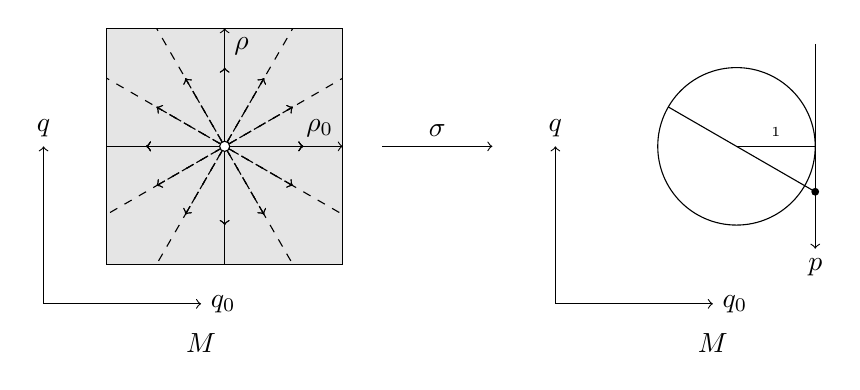
\begin{tikzpicture}
    \draw[->] (0, 0) -- (2, 0) node[anchor=west] {$q_0$};
    \draw[->] (0, 0) -- (0, 2) node[anchor=south] {$q$};
    
    \node (m) at (2.3, 2) {};
    
    \filldraw[draw=black, fill=gray!20] (m) ++(-1.5, -1.5) -- ++(0, 3) -- ++(3, 0) -- ++(0,-3) -- cycle;
    \draw[->] (m) ++(-1.5, 0) -- ++(3, 0) node[anchor=south east] {$\rho_0$};
    \draw[->] (m) ++(0, -1.5) -- ++(0, 3) node[anchor=north west] {$\rho$};
        
    \begin{scope}
        \clip (m) ++(-1.5,-1.5) rectangle ++(3, 3);
        \foreach \i in {0,30,...,180}{
            \draw[<->, dashed] (m) ++({-cos(\i)}, {-sin(\i)}) -- ++({2*cos(\i)}, {2*sin(\i)});
        }
        \foreach \i in {0,30,...,180}{
            \draw[<->, dashed] (m) ++({-cos(\i)}, {-sin(\i)}) -- ++({2*cos(\i)}, {2*sin(\i)});
        }
        \foreach \i in {0,30,...,180}{
            \draw[dashed] (m) ++({-4*cos(\i)}, {-4*sin(\i)}) -- ++({8*cos(\i)}, {8*sin(\i)});
        }
    \end{scope}
    
    \node[circle,draw=black,fill=white,inner sep=1.3pt] at (m) {};
    
    \draw[->] (6.5, 0) -- (8.5, 0) node[anchor=west] {$q_0$};
    \draw[->] (6.5, 0) -- (6.5, 2) node[anchor=south] {$q$};
    
    \node[fill=none] (m2) at (8.8, 2) {};
    
    \draw (m2) circle (1);
    \draw[->] (m2) ++(1, 1.3) -- ++(0, -2.6) node[anchor=north] {$p$} ;
    \draw (m2.center) ++(-0.866, 0.5) -- (9.8, 1.423) node[circle,fill=black, inner sep = 1pt] {};
    \draw (m2.center) -- ++(1, 0) node[pos=0.5,anchor=south] {\tiny{1}};
    %\draw[->] (m) ++(-1.5, 0) -- ++(3, 0) node[anchor=west] {$\rho_0$};
    %\draw[->] (m) ++(0, -1.5) -- ++(0, 3) node[anchor=south] {$\rho$};
    
    \draw[->] (4.3, 2) -- (5.7, 2) node[pos=0.5,anchor=south] {$\sigma$};
     
    \node at (2, -0.5) {$\ctzbundle{M}$};
    \node at (8.5, -0.5) {$\pctbundle{M}$};
\end{tikzpicture}

    \end{center}
    \caption{Illustration of the principal $\mgroup$-bundle $\bundle{\ctzbundle{M}}{\pi}{\pctbundle{M}}$. The total space $\ctzbundle{M}$ is the cotangent bundle to $M$ with zero section removed, which is shown on the left. The action by the multiplicative group $\mgroup$ is illustrated by the arrows, for it acts as a scaling (dilation) on all the cotangent variables. The origin is not part of the fiber, for it is part of the zero section. The bundle projection $\pi$ projects all points that are on the same orbit (straight lines through the origin) to a single point on the base manifold: the projectivized cotangent bundle $\pctbundle{M}$. The former space has a symplectic structure while the latter space has a contact structure. Observe from \cref{eq:homo_coords} that $p = \rho/\rho_0$, i.e. such that $p$ is a coordinate for the projectivization by stereographic projection, as shown on the right.}
    \label{fig:principal_bundle}
\end{figure}

Define the \mgroup-\emph{action} $\raction{}$ on $\ctzbundle{M}$ as:
$$ \raction: \ctzbundle{M}\times\mgroup \to \ctzbundle{M} : \quad (q_0, q, \rho_0, \rho) \blacktriangleleft \lambda = (q_0, q, \lambda \rho_0, \lambda \rho ) \qquad \lambda \in \mgroup,$$
which are referred to as dilations of the fiber.

As illustrated in \cref{fig:principal_bundle}, the \emph{orbit space} of $\ctzbundle{M}$ with respect to the group action $\raction{}$ is the space of all points in $\ctzbundle{M}$ with all points on the same line through the origin (in the fiber) identified. This space is precisely equal to the projectivization of the cotangent bundle $\pctbundle{M}$. Hence, consider the \emph{principal} $\mgroup$-bundle $\bundle{\ctzbundle{M}}{\sigma}{\pctbundle{M}}$ 
\begin{center}
    \begin{tikzcd}
        \ctzbundle{M} \\ \ctzbundle{M} \arrow[u, "\raction{\mgroup}"] \arrow[d, "\sigma"] \\ \pctbundle{M} \cong \cbundle{M}
    \end{tikzcd}
\end{center}
The removal of the zero section is required for the group action to be free. The principal bundle $\bundle{\ctzbundle{M}}{\pi}{\pctbundle{M}}$ admits a \emph{fibered symplectic Liouville structure}, given by the Liouville form \cite{Libermann1987}
$$ \theta = \rho_0\dd{q_0} + \rho\dd{q}, $$
and the associated two-form $\omega = -\dd{\theta}$. The distinctive feature of these forms that makes this a Liouville structure is that they both commute with the group action $\raction{}$: \cite{Libermann1987}
$$ (\raction{\lambda})^* \theta = \lambda \theta \qquad \lambda \in \real_*,$$
which makes them homogeneous forms of degree 1.

The projection map $\sigma$ of the principal bundle is locally defined as 
\begin{equation}
    \sigma : \ctzbundle{M} \to \pctbundle{M}: (q_0, q, \rho_0, \rho) \mapsto (q_0, q, -\rho/\rho_0), 
    \label{eq:principal_projection}
\end{equation}
with $p \equiv -\rho/\rho_0$ a coordinate for the projectivized fiber. This coordinate does not cover the entire fiber: the points for which $\rho_0 = 0$ is missing (in \cref{fig:principal_bundle}, this point is the only point on the circle that cannot be projected on the $p$-axis). However, we will make the deliberate assumption that in our application, $\rho_0$ is never equal to zero.
%The manifold $\ctzbundle{M}$ is called the symplectization of the contact manifold. For now, we have not assigned any specific meaning to the coordinates given above, but they will turn out to match with the notation used in \cref{eq:lag_CK,eq:ham_CK}, etc.

Finally, the \emph{Liouville vector field} $Z$ associated with the Liouville structure is the vector field that represents the dilation of the fiber in the symplectization. It is defined as
\begin{equation}
    Z = \fromDual{\omega}(\theta) = \rho_0\pdv{}{\rho_0} + \rho\pdv{}{\rho}. 
    \label{eq:liouville_vf}
\end{equation}
Vector field (components) colinear with the Liouville vector fields are called \emph{vertical}; they represent dissipative action in the system. After the vertical components are removed, they remaining vector field is called \emph{horizontal}.

[Liouville automorphisms, commute with the Liouville vector field -> very important in the chapter about split-quaternions]

To summarize, we lifted the original system with symplectic structure $\wedgep{\dd{q}}{\dd{p}}$ to a contact manifold through the addition of a gauge variable $q_0$. We then symplectified the contact manifold to a four-dimensional system, with `positions' $(q_0, q)$ and `momenta' $(\rho_0, \rho)$.

\subsection{Homogeneous Hamiltonian systems} The theoretical construction of the past section serves an important purpose, because it is the symplectified space which is the proper setting for the Caldirola-Kanai Hamiltonian discussed in \cref{sec:caldirola}. Along with the symplectification of the contact structure described in the past section, we can do the same with a contact Hamiltonian system.

There is a one-to-one correspondence between contact Hamiltonians on $\pctbundle{M}$ and a special class of Hamiltonians on the symplectified space $\ctzbundle{M}$. These are the Hamiltonians which are \emph{homogeneous} in the cotangent variables with degree 1:\footnote
{This is a consequence of the Euler theorem for homogeneous functions. If $\mathscr{H} = \mathscr{H}(\vec{q}, \vec{\rho})$ is homogeneous of degree $r$ in $\vec{\rho}$, then
    $$ \sum_{i = 1}^n \rho_i \pdv{\mathscr{H}}{\rho_i} = r \mathscr{H}. $$
 Therefore, for homogeneity of degree 1, we have: 
 $$ \lied{Z}{\mathscr{H}} = Z(\mathscr{H}) = \sum_{i=1}^n \rho_i \pdv{\mathscr{H}}{\rho_i} = \mathscr{H} \quad \text{with}\quad Z \equiv \sum \rho_i \pdv{}{\rho_i}. $$
 The correspondence between the 
}
\begin{equation}
    \mathscr{H}(q_0, q, \lambda \rho_0, \lambda \rho) = \lambda\,\mathscr{H}(q_0, q, \rho_0, \rho) \quad \text{or} \quad \lied{Z}{\mathscr{H}} = \mathscr{H},
\end{equation}
with $\lambda \in \real_0,\: H \in \functions{\ctzbundle{M}}$ and $Z$ defined according to \cref{eq:liouville_vf}. Given that $H$ is indeed homogeneous of degree 1, this correspondence is in canonical coordinates:
\begin{equation}
    \mathscr{H}(q_0, q, \rho_0, \rho) = -\rho_0\,H\qty(q_0, q, -\frac{\rho}{\rho_0})
    \label{eq:H_correspondence}
\end{equation}
where $\mathscr{H} \in \functions{\ctzbundle{M}}$, $H \in \functions{\pctbundle{M}}$ and $p = -\rho / \rho_0$ is a coordinate for the projectivized fiber. Likewise, there is also a direct correspondence between the vector fields generated by these Hamiltonians, and therefore the system dynamics. This is the reason why we go through the trouble of symplectification in the first place, it offers significant computational advantages. It is possible to derive the contact equations directly (as \citet{Bravetti2017} does), but it does not offer the same amount of insight as its symplectified counterpart. \cite{VanderSchaft2021a,Arnold1989}

Now, recall the Caldirola-Kanai Hamiltonian in \cref{eq:ham_CK}. Instead of assuming a direct time-dependence, we will think of the time-dependence as the gauge momentum, i.e. $\rho_0 \:``=" -\ec^{\gamma t}$. However, we will now consider $\rho_0$ to be a coordinate in its own right, instead of directly using the expression above --- the equality sign must therefore not be taken too literally. The Caldirola-Kanai Hamiltonian is then written as (cf. \cref{eq:ham_CK}):
$$ -\rho_0 \qty[\frac{1}{2m}\qty(-\frac{\rho}{\rho_0})^2 + \frac{1}{2}kq^2]. $$
The motivation to make this particular choice is twofold: first, observe that $\mathscr{H}$ is homogeneous in the cotangent variables $\rho_0, \rho$, and second, that their fraction yields the \emph{real} momentum: $ p = -\rho/\rho_0 $. However, we must acknowledge a potential dependence on $q_0$, since we want to convert the explicitly time-dependent Hamiltonian into a contact Hamiltonian. We therefore add the arbitrary function $f = f(q_0)$, whose value is to be determined later, and also multiply by $\rho_0$ to maintain homogeneity. The homogeneous Hamiltonian $\mathscr{H}$ is then:
\begin{equation}
    \mathscr{H}: \ctzbundle{M} \to \real: \quad \mathscr{H}(q_0, q, \rho_0, \rho) = -\rho_0 \qty[\frac{1}{2m}\qty(-\frac{\rho}{\rho_0})^2 + \frac{1}{2}kq^2 + f(q_0)]. 
    \label{eq:homo_hck}
\end{equation}
 Using the correspondence given by \cref{eq:H_correspondence}, the homogeneous Hamiltonian may be `projected' to the contact Hamiltonian $H$:
\begin{equation}
    H: \pctbundle{M} \to \real: \quad H(q_0, q, p) = \frac{p^2}{2m} + \frac{1}{2}kq^2 + f(q_0).
\end{equation}
Numerically, this contact Hamiltonian is the same as the Hamiltonian for an undamped mass-spring system but it is defined on the contact manifold that also takes into account the gauge variable $q_0$.

\emph{Equations of motion} Now to derive the equations of motion. As mentioned, this is easiest in the symplectified space because Hamilton's equations can be readily applied (the reader can consult \cref{app:contact_geometry} for the direct derivation). Because we are using canonical coordinates, the Hamiltonian vector field
\begin{equation}
    X_\mathscr{H} = \fromDual{\omega}(\dd{\mathscr{H}})
    \label{eq:ham_vf}
\end{equation}
corresponds to Hamilton's equations in the familiar form:
\begin{equation}
    \dv{\rho}{t} = -\pdv{\mathscr{H}}{q},\quad
        \dv{\rho_0}{t} = -\pdv{\mathscr{H}}{q_0},\quad
        \dv{q}{t} = \pdv{\mathscr{H}}{\rho},\quad
        \dv{q_0}{t} = \pdv{\mathscr{H}}{\rho_0}.
\end{equation}
Observe that this motivates why one has to take the partial with respect to the `other' momentum in the Caldirola-Kanai momentum: we are dealing with a specific instance of a more general class of homogeneous coordinates of the cotangent variables. Of course, the variable of interest is the actual momentum $p$, not the scaled version $\rho$. The time-derivative of $p$ can be written in terms of $\rho$ and $\rho_0$, completely analogous to \cref{eq:momentum_relation}:
\begin{equation}
    p = -\rho/\rho_0 \quad\Rightarrow\quad \dv{p}{t} = -\frac{1}{\rho_0}\dv{\rho}{t} + \frac{\rho}{\rho_0^2}\dv{\rho_0}{t} = -\frac{1}{\rho_0}\dv{\rho}{t} - \frac{p}{\rho_0}\dv{\rho_0}{t}. 
    \label{eq:homo_momenta}
\end{equation}
Given \cref{eq:homo_hck}, the partial derivatives of $\mathscr{H}$ and $H$ are related through the by relations: \cite{Arnold1989}
\begin{equation}
    \begin{split}
        \pdv{\mathscr{H}}{q} &= -\rho_0 \pdv{H}{q}, \\
        \pdv{\mathscr{H}}{q_0} &= -\rho_0 \pdv{H}{q_0}, \\
        \pdv{\mathscr{H}}{\rho} &= -\rho_0 \pdv{H}{p}\pdv{p}{\rho} = \pdv{H}{p}, \\
        \pdv{\mathscr{H}}{\rho_0} &= -H - \rho_0 \pdv{H}{p}\pdv{p}{\rho_0} = -H - \pdv{H}{p}\frac{\rho}{\rho_0} = \pdv{H}{p}p - H.\\
    \end{split}
    \label{eq:partial_relation}
\end{equation}
Hence, the \emph{contact} equations of motion can be found by combining of \cref{eq:momentum_relation} and \cref{eq:partial_relation}:
\begin{equation}
    \begin{split}
        \dv{q}{t} &= \pdv{H}{p} \\
        \dv{p}{t} &= \frac{1}{\rho_0}\pdv{\mathscr{H}}{q} + \frac{p}{\rho_0}\pdv{\mathscr{H}}{q_0} = - \pdv{H}{q} - p\pdv{H}{q_0} \\
        \dv{q_0}{t} &= \pdv{H}{p}p - H.
    \end{split}
    \label{eq:contact_eom}
\end{equation}
Some observations are important to note:
\begin{itemize}
    \item The evolution of the position $q$ remains the same as for the `normal' (undamped) case.
    \item The evolution of the momentum operator picks up a term that is depends on presence of the gauge variable in the contact Hamiltonian.
    \item The evolution of the gauge variable is equal to the Legendre transformation of the contact Hamiltonian with respect to $p$.
\end{itemize}

We are now ready to determine the nature of the as of yet unknown function $f$ to obtain the correct equations of motion. By comparing \cref{eq:homo_momenta} and \cref{eq:contact_eom}, the following relation must hold:
$$ \frac{1}{\rho_0}\dv{\rho_0}{t} = \pdv{H}{q_0} = \dv{f}{q_0}. $$
Furthermore, since we initial `substituted' $\ec^{\gamma t}$ in favor of $\rho_0$, the left hand side of the equation should be equal to $\gamma$ for it to be consistent with the Caldirola-Kanai Hamiltonian. Hence, we know that $\dv{f}{q_0} = \gamma$, or $f(q_0) = \gamma q_0$ up to a constant, which we choose to be zero. Although this may seem like an odd construction, the only thing we did is made the contact equation of motions equivalent with the time-dependent equations of motion. Now, the fact that $\rho_0 = \ec^{\gamma t}$, ceases to be an a priori assumption, and is derivable through Hamilton's equations:
$$ \dv{\rho_0}{t} = -\pdv{\mathscr{H}}{q_0} = \gamma\rho_0 \quad \Rightarrow \quad \rho_0 = \ec^{\gamma t} + C$$

As such, we have for the contact Hamiltonian:
\begin{equation}
    H: \pctbundle{M} \to \real: \quad H(q_0, q, p) = \frac{p^2}{2m} + \frac{1}{2}kq^2 + \gamma q_0,
    \label{eq:H_dho}
\end{equation}
and this is precisely Bravetti's result. For the homogenous Hamiltonian on the symplectified space, we have:
\begin{equation}
    \mathscr{H}: \ctzbundle{M} \to \real: \quad \mathscr{H}(q_0, q, \rho_0, \rho) = -\rho_0\,\qty[\frac{1}{2m}\qty(-\frac{\rho}{\rho_0})^2 + \frac{1}{2}kq^2 + \gamma q_0]. 
    \label{eq:H_dho_homo}
\end{equation}
%It is easily verified that the contact Hamilton equations $\cref{eq:contact_eom}$ yield the correct equations of motion for the damped harmonic oscillator:
%$$ \dv{q}{t} = p/m \qquad \dv{p}{t} = -kq -\gamma p.$$
%On the other hand, the equation of motion for $q_0$ requires some additional considerations; this is the subject of the next section.

The Hamiltonian vector field $X_\mathscr{H} \in \vfields{\ctzbundle{M}}$ is then, using \cref{eq:H_dho_homo} and \cref{eq:ham_vf}:
$$ X_{\mathscr{H}} = \frac{p}{2m}\pdv{}{q}\: + \: \qty[\frac{1}{2m}\qty(\frac{\rho}{\rho_0})^2 - \frac{1}{2}kq^2 - \gamma q_0]\pdv{}{q_0}\: + \: \rho_0 kq \pdv{}{\rho}\: + \: \gamma \rho_0 \pdv{}{\rho_0}.$$ 

The contact Hamiltonian vector field $X_H \in \vfields{\pctbundle{M}}$ is obtained either by using the contact Hamilton equations given by \cref{eq:contact_eom}, or by using the pushforward of the projection map $\sigma$:
$$ X_H = \sigma_*\,X_\mathscr{H} = \frac{p}{2m}\pdv{}{q}\: + \: \qty(\frac{p^2}{2m} - \frac{1}{2}kq^2 - \gamma q_0)\pdv{}{q_0}\: - \: (kq + \gamma p)\pdv{}{p}\: $$
This is essentially the equivalent of the time-dependent transformation performed in \cref{sec:caldirola}. Clearly, these yield the correct equations of motion for the damped harmonic oscillator.

\paragraph{Mechanical energy} One of the computational advantages of the symplectified space is the fact that `regular' Poisson brackets can be used in contrast to their slightly unwieldy contact counterparts.\footnote
{The Poisson bracket is defined as 
    $$ \poisson{f}{g} = \omega(X_f, X_g) = \lied{X_g}{f},$$
 where $X_f$ and $X_g$ are the Hamiltonian vector fields of $f$ and $g$. \cite{Libermann1987}
} 
Define therefore a lift that takes functions from the contact manifold to the symplectified manifold:
$$ 
    \ell : \functions{\pctbundle{M}} \to \functions{\ctzbundle{M}}: \quad g \mapsto g \circ \sigma,
$$
with $\sigma$ as in \cref{eq:principal_projection}. The function takes the same value but is expressed in terms of the coordinates of the symplectified space.

The mechanical energy, denoted by $E$, is equal to 
$$ E: \pctbundle{M} \to \real: \quad E(q_0, q, p) = \frac{p^2}{2m} + \frac{1}{2}kq^2,$$
which can be lifted to the symplectified space
$$ 
    \ell(E)(q_0, q, \rho_0, \rho) = \frac{1}{2m}\qty(-\frac{\rho}{\rho_0})^2 + \frac{1}{2}kq^2.
$$
The change of mechanical energy in the system is then readily determined using the Poisson brackets:
$$ \dv{E}{t} = \poisson{\ell(E)}{\mathscr{H}} = \lied{X_\mathscr{H}}{\ell(E)} = -\frac{\gamma}{2m}\qty(\frac{\rho}{\rho_0})^2 = -\frac{\gamma}{2m}p^2,$$
which is precisely the dissipative power in the damping element.

\todo{Check minus signs of the change in mechanical energy, should be opposite to heat generated.}
\todo{Finish Poincaré lemma discussion.}

\begin{mathbox}{The importance of the zero section}
    It may be tempting to disregard the removal of the zero section from the cotangent bundle as a mathematical technicality. It has, however, deep implications for the nature of the Hamiltonian systems that can be defined on it, encoded in the so-called de Rham cohomology groups.
    
    Suppose that $Y$ is a symplectic vector field with $\omega$ the symplectic form. The 1-form
    $$\xi = \intpr{Y}{\omega}$$
    is necessarily closed, because
    $$ \dd{\intpr{Y}{\omega}} \; = \underbrace{\bcancel{\lied{Y}{\omega}}}_{Y \text{ symp.}}\;- \; \underbrace{\bcancel{\intpr{Y}{\dd{\omega}}}}_{\omega \text{ closed}}\; = 0. $$
    The Poincaré lemma (a specific instance of the de Rham cohomology) says that on a \emph{contractible domain}, all closed forms are necessarily also exact (the converse is true on any manifold, for $\dd{}^2 = 0$). This would mean that, if $\xi$ were to be defined on a contractible manifold, it would automatically be an exact form (this is the same as saying that on these types of manifolds, all symplectic vector fields are Hamiltonian). In other words, there must be a function $\mathscr{H}$ such that $\xi = \dd{\mathscr{H}}$.

    Integration around curve to show that $\xi$ in our case is not exact. Hard, because over two charts.

    Also show that the region of interest is not simply connected in order to use de Rham in the first place.
    $ \real^4 / \{(q_0, q, 0, 0)\} $ not simply connected
\end{mathbox}

\subsection{Physical interpretation of the gauge variables}
Another advantage of using the purely symplectic formalism on the lifted space is the fact that the homogeneous Hamiltonian is invariant under the flow it generates, since the explicit time-dependence has been removed:
$$ \dv{\mathscr{H}}{t} = \poisson{\mathscr{H}}{\mathscr{H}} = \lied{X_{\mathscr{H}}}{\mathscr{H}} = 0. $$
We may therefore associate the homogeneous Hamiltonian with a constant. By inspection of \cref{eq:H_correspondence}, 
$$ \mathscr{H}(q_0, q, \rho_0, \rho) = -\rho_0\,\underbrace{\qty(C\rho_0^{-1})}_{\ell(H)} \qquad C \in \real.$$
Recall that we made the assumption earlier that $\rho_0$ is a function \emph{without zeros}. 

The constant $C$ is a degree of freedom in the system that we are free to choose, for the equations of motion will be consistent with any chosen value. This called a \emph{gauge} of the system, and its choice will influence the value of the gauge variable directly. The contact Hamiltonian is not a constant of motion however (at least, for dissipative systems). With some abuse of notation
$$ \dv{H}{t} = C\,\dv{\rho_0}{t}  = -C\,\pdv{\mathscr{H}}{q_0}.$$
Until now, there were no assumptions regarding the value of the damping constant $\gamma$: indeed, the `normal' equations of motion are readily derived when $\gamma$ is set to zero. We will now add the assumption that there is at least some dissipation present in the system ($\gamma \neq 0$) to assign further intrepretation to the gauge variable. The evolution of $q_0$ is directly related to the evolution of $H$ by \cref{eq:H_dho}
$$ 
    q_0 = \frac{1}{\gamma} \bigg(\rho_0 C - \underbrace{\frac{p^2}{2m} - \frac{1}{2}kq^2}_{E}\bigg)
$$
Because we are free to choose the value of $C$, let us now make a choice of particular interest; namely $C = 0$. In that case, both $\mathscr{H}$ and $H$ vanish \emph{weakly};\footnote
{The weak equality, as opposed to the strong equality, is not maintained under variations. Hence, although the numerical value of the function is zero, its partial derivatives do not necessarily vanish. The reader is referred to \citet{Dirac1950} for a more elaborate discussion.}
this choice rids us from the additional freedom in $C$ that would also show up in the equation of motion for $q_0$. Instead, $q_0 = - E/\gamma$; which can be interpreted as the heat dissipated by the system (one can add a suitable initial condition for $q_0(0) = E(0)$ to make this also numerically correct). This `heat' function will be called $Q$; we therefore have
$$ q_0 = Q/\gamma. $$
The vanishing of the Hamiltonians reflects the energy balance that is maintained throughout the evolution of the system:
\begin{equation*}
    \begin{split}
        H &= E + Q \\
          &= \text{\textsc{mechanical energy}} + \text{\textsc{dissipated heat}}.
    \end{split}
\end{equation*}
The fact that $H$ vanishes makes it a constant of motion on par with the symplectified Hamiltonian $\mathscr{H}$. This careful choice of for the gauge variable removes a lot of the ambiguity that is naturally present in contact systems; this rather subtle point is a bit overlooked by past research. \cite{Bravetti2017} 
Furthermore, the evolution of the dissipated heat is
$$ \dv{Q}{t} = \gamma \dv{q_0}{t} = \gamma \qty[\frac{1}{2m}\qty(\frac{\rho}{\rho_0})^2 - \frac{1}{2}kq^2 - \gamma q_0] = \gamma\frac{1}{2m}\qty(\frac{\rho}{\rho_0})^2, $$
which is the expected result.

This very particular choice for the gauge variable may seem a little arbitrary. However, \emph{in general}, the time-rate of change
$$
    \jacobi{f}{g}
$$

\todo{Canonical transformation}
\todo{Action-angle coordinates}
\todo{Generalization using Jacobi problems}


\section{Legendre involution}
In the classic, symplectic case, the Legendre transformation is used to pass from the Hamiltonian to the Lagrangian formalism and vice versa. This is because the Legendre transform facilitates a mapping between the tangent and cotangent bundle. If the Lagrangian (or Hamiltonian) is (hyper)regular (i.e. the mass matrix is invertible), this mapping is a diffeomorphism. \cite{Carinena1990}

One would be tempted to use the normal Legendre transformation on the symplectified Hamiltonian $\mathscr{H}$. This approach will meet some problems though:
\begin{itemize}
    \item A homogeneous function is not regular in the homogeneous variables --- naturally, a degree of freedom still resides in the action of the multiplicative group. Therefore, the mapping from the cotangent to the tangent bundle is not a diffeomorphism. Said otherwise, there is not a one-to-one correspondence between the homogeneous momenta and the associated velocities in the Lagrangian description.
    \item As a consequence of Euler's theorem for homogeneous functions, the Legendre transformation for a homogeneous function is necessarily equal to zero. For any homogeneous function $H$ (of degree 1), Euler's theorem states that
    $$ \sum_{i = 1}^n \rho_i \pdv{\mathscr{H}}{\rho_i} = \mathscr{H}, $$

        i.e. the function is equal to its associated `action', and therefore the expression for the Legendre transformation vanishes. \cite{Dirac1950,Dirac1933}
\end{itemize}
There is a better path to take. In essence the Legendre transform is (and was originally meant to be) a \emph{contact transformation}.

\section{Notes}

\begin{mathbox}{Lie derivatives \& Max' question}
    The Lie derivative of the tautological form $\alpha = p\dd{q}$ with respect to the
    Hamiltonian vector field
    $$ X_H = \pdv{H}{p}\pdv{}{q} - \pdv{H}{p}\pdv{}{p}$$
    is denoted by
    $$ \lied{X_H}{\alpha}.$$
    Using Cartan's magic formula ($ \lied{V}{\theta} = \dd{(\intpr{V}{\theta})} + \intpr{V}{\dd{\theta}}$), this expression
    can be written as
    \begin{equation*} 
        \begin{split}
            \lied{X_H}{p\dd{q}} &= \dd{(\intpr{X_H}{p\dd{q}})} + \intpr{X_H}{\dd{(p\dd{q})}} \\
                                &= \dd{(\intpr{X_H}{p\dd{q}})} - \intpr{X_H}{\omega} \\
                                &= \dd{(\intpr{X_H}{p\dd{q}})} - \dd{H} \\
                                &= \dd{\qty(\pdv{H}{p}p)} - \dd{H} \\
                                &= \dd{(\dot{q}p)} - \dd{H} \\
                                &= \dd{(\dot{q}p - H)} \\
                                &= \dd{L} \\
        \end{split}
    \end{equation*}

    Explicitly in components:
    \begin{equation*}
        \lied{X_H}{\alpha} = \qty[X_H^{\nu}(\partial_{\nu}\alpha_{\mu}) + (\partial_{\mu} X_H^{\nu})\alpha_{\nu}]\dd{x}^{\mu}
    \end{equation*}

    \begin{equation*}
        \begin{split}
            \lied{X_H}{\alpha} =\, &\qty[\pdv{H}{p}\qty(\pdv{}{q}p) + \qty(\pdv{}{q}\pdv{H}{p})p - \pdv{H}{q}\qty(\pdv{}{p}p) - \qty(\pdv{}{q}\pdv{H}{q})0]\dd{q} \\
                                + &\qty[\pdv{H}{p}\qty(\pdv{}{q}0) + \qty(\pdv{}{p}\pdv{H}{p})p - \pdv{H}{q}\qty(\pdv{}{q} 0) - \qty(\pdv{}{p}\pdv{H}{q})0]\dd{p} \\
                               =\,&\qty[ \qty(\pdv{}{q}\pdv{H}{p})p - \pdv{H}{q}]\dd{q} + \qty[\qty(\pdv{}{p}\pdv{H}{p})p]\dd{p}\\
        \end{split}
    \end{equation*}
    Compare this with the expression using the Cartan equation:
    \begin{equation*}
        \begin{split}
            \dd{\qty(\pdv{H}{p}p - H)} &= \pdv{}{q}\qty(\pdv{H}{p}p)\dd{q} + \pdv{}{p}\qty(\pdv{H}{p}p)\dd{p} - \pdv{H}{q}\dd{q} - \pdv{H}{p}\dd{p}\\
                                       &= \qty[p\pdv{}{q}\qty(\pdv{H}{p}) + \pdv{H}{p}\pdv{p}{q} - \pdv{H}{q}]\dd{q} + \qty[p\pdv{}{p}\qty(\pdv{H}{p}) + \pdv{H}{p}\pdv{p}{p} - \pdv{H}{p}]\dd{p}
        \end{split}
    \end{equation*}
    which coincides with the previous expression.

\end{mathbox}



\chapter{Split-Quaternions as Dynamical Systems}
\label{chap:quaternion}
%\lsymb{$\vec{\alpha}$}{A differential form}

In this chapter, the geometric connection is made between the algebra of split-quaternions and the qualitative behavior of two-dimensional linear dynamical systems. 

\section{Split-quaternion algebra}
\subsection{Basic properties}
Like conventional quaternions, the split-quaternions form a number system that consists of linear combinations of four basis elements, which will be denoted by 1, \quati, \quatj and \quatk.\footnote
{Even though they behave similarly, the imaginary unit $\ii$ is not to be confused with the split-quaternion basis element \quati, because they belong to different number systems.}
The algebra of split-quaternions is associative but not commutative --- formally speaking, we are dealing with an algebraic structure called a \emph{noncommutative ring}. The multiplication table for the split-quaternion algebra is shown in \cref{tab:quat_table}. The set of split-quaternions is denoted by \spquaternions, since \quaternions is reserved for conventional quaternions.\footnote
{The `$\mathbb{H}$' is in honour of sir William Rowan Hamilton, who also developed the Hamiltonian formalism: the fruits of his work truly form the central theme in this thesis. \cite{Stillwell2008}}
\begin{table}[ht!]
    \centering
    \caption{Multiplication table for the split-quaternion algebra.}
    \label{tab:quat_table}
    \begin{tabular}{c|cccc}
        \toprule
        &         1      & \quati  & \quatj  & \quatk \\ 
        \midrule
        1       & 1      & \quati  & \quatj  & \quatk \\ 
        \quati  & \quati & -1      & \quatk  & -\quatj \\ 
        \quatj  & \quatj & -\quatk & 1       & -\quati \\ 
        \quatk  & \quatk & \quatj  & \quati  & 1 \\ 
        \bottomrule
    \end{tabular}
\end{table}

The important distinction from conventional quaternions resides in the diagonal elements of \cref{tab:quat_table}. For quaternions, all the nonreal basis elements square to $-1$, this is not the case for the split-quaternions (only \quati does). This is precisely the reason why split-quaternions are `split', for this difference in sign makes their norm (to be defined later) into an indefinite form. That is to say, whereas quaternions have a `metric signature' (in a very imprecise sense of the word metric) of $(+, +, +, +)$, for the split-quaternions we have $(+, +, -, -)$. The distinctive `metric' signature makes the algebra of split-quaternions  different from its conventional quaternion counterpart.

\paragraph{Dihedral group} The basis elements of the split-quaternions $\qty{1, \quati, \quatj, \quatk}$ form a finite group under multiplication, namely the \emph{dihedral group} \digroup{4}, which represents all the symmetries of a square: the identity, a 90-degree rotation and two reflections, as illustrated in \cref{fig:square_symmetry}. \cite{Dummit2004}
\begin{figure}[h!]
    \centering
    \begin{tikzpicture}
    \node[draw, inner sep=3mm,thick, fill=accent1!40] at (0, 0) {};
    \node[draw, inner sep=3mm,thick, fill=accent1!40] at (2, 0) {};
    \node[draw, inner sep=3mm,thick, fill=accent1!40] at (4, 0) {};
    \node[draw, inner sep=3mm,thick, fill=accent1!40] at (6, 0) {};
    \draw[->] (2, 0.7) arc (90:0:0.7);
    \draw[->] (2, -0.7) arc (270:180:0.7);
    \draw[dashdotted] (3.5, 0.5) -- (4.5, -0.5);
    \draw[<->] (3.75, -0.25) -- (4.25, 0.25);
    \draw[dashdotted] (5.5, -0.5) -- (6.5, 0.5);
    \draw[<->] (5.75, 0.25) -- (6.25, -0.25);
    \node[] at (0, -1.1) {1};
    \node[] at (2, -1.1) {\quati};
    \node[] at (4, -1.1) {\quatj};
    \node[] at (6, -1.1) {\quatk};

\end{tikzpicture}

    \caption{The dihedral group \digroup{4} is the symmetry group of a square. This group is isomorphic to the group formed by $1, \quati, \quatj$ and \quatk under multiplication.}
    \label{fig:square_symmetry}
\end{figure}

The structure of the dihedral group can be visualized by its \emph{cycle graph} in \cref{fig:cycle_graph}. Many important properties of the split-quaternion algebra and the applications in this chapter can be traced back to the shape of this cycle graph. One example is the split nature of the quaternions: the \quati-element generates an order-4 cycle, while \quatj and \quatk generate order-2 cycles (in contrast, the cycle graph for conventional quaternions is entirely symmetric for all these elements). \cite{Dummit2004}
\begin{figure}[h!]
    \centering
    \begin{tikzpicture}
    \node[draw, thick, circle, fill=accent1!40] (e) at (0, 0) {};
    
    \node[thick, draw, circle, below right=0.8cm and 0.5cm of e] (r1) {};
    \node[thick, draw, circle, below left=0.8cm and 0.5cm of e] (r2) {};
    \node[thick, draw, circle, left of= r2] (r3) {};
    \node[thick, draw, circle, right of= r1] (r4) {};
    \node[thick, draw, circle, above=1.5cm of e] (ro2) {};
    \node[thick, draw, circle, above right=0.7cm and 1cm of e] (ro1) {};
    \node[thick, draw, circle, above left=0.7cm and 1cm of e] (ro3) {};
    
    \draw[thick] (e) -- (r1);
    \draw[thick] (e) -- (r2);
    \draw[thick] (e) -- (r3);
    \draw[thick] (e) -- (r4);
    
    \draw[thick] (e) -- (ro1) -- (ro2) -- (ro3) -- (e);

\end{tikzpicture}

    \caption{Cycle graph of the dihedral group. There are five cycles: one of order four which represents the rotations (or the element \quati), and four order-2 cycles, which are all the possible reflections. The colored element represents the identity.}
    \label{fig:cycle_graph}
\end{figure}

\paragraph{Split-quaternion norm} Complex numbers have a real and imaginary part. Likewise, (split)-quaternions have a similar notion: a \emph{scalar} (or real) and \emph{vector} (or imaginary) components. For an arbitrary split-quaternion $a \in \spquaternions$, \cite{Jafari2014}
$$ a = \quat{a_0}{a_1}{a_2}{a_3} $$
the real part is $\scapart{h} = a_0$ and the vector part is $ \vecpart{a} = \quatvec{a_1}{a_2}{a_3}$. For convenience, the vector part will be referred to in traditional bold vector notation:
$$ \vec{a} \equiv \vecpart{a} \equiv \quatvec{a_1}{a_2}{a_3}. $$

Furthermore, for every split-quaternion there is a unique \emph{conjugate}
$$ \conj{a} = \scapart{a} - \vecpart{a} = a_0 - a_1\quati - a_2\quatj - a_3\quatk, $$
which we require to define the \emph{squared split-quaternion norm}:
\begin{equation}
    \mathscr{N}:\;\spquaternions \to \real:\;\;\mathscr{N}(a) \equiv a\conj{a} = a_0^2 + a_1^2 - a_2^2 - a_3^2. 
    \label{eq:quat_norm}
\end{equation}
As mentioned, this norm is not positive definite, in stark contrast to quaternions (or complex numbers, for that matter). Split-quaternions can be categorized into three regimes based on their norm being negative, zero or positive. In the tradition of special relativity, these regimes are named\footnote
{Spacetime is also four-dimensional, but the signature of the Minkowski metric is different from the split-quaternion signature: it is either $(-, +, +, +)$ or equivalently $ (+, -, -, -)$ depending on the sign convention one chooses to follow. However, the terminology (i.e. spacelike, timelike, lightlike) still applies.} \cite{Misner1970,Landau1971}
\begin{itemize}
    \item \emph{timelike} if $ \mathscr{N}(a) > 0 $,
    \item \emph{lightlike} if $ \mathscr{N}(a) = 0 $, 
    \item \emph{spacelike} if $ \mathscr{N}(a) < 0 $.
\end{itemize}
The \emph{split-quaternion norm} is then defined as
$$ \norm{a} \equiv \sqrt{\abs{\mathscr{N}(a)}}. $$

\paragraph{Vector norm}
Apart from the split-quaternion norm, we may also define a (square) norm that only considers the \emph{vector part} of the split-quaternion. This squared norm is defined in accordance with the overall squared split-quaternion norm given by \cref{eq:quat_norm}:
$$ \mathscr{N}(\vec{a}) = a_1^2 - a^2_2 - a^2_3. $$
The notation used here is not abusive: $\vec{a}$ simply refers to the split-quaternion with the same vector part as $a$ but with zero scalar part. We can therefore use the same function with no ambiguity. Likewise, the vector norm is $ \norm{\vec{a}} = \sqrt{\abs{\mathscr{N}(\vec{a})}} $. 

The quadratic form of the squared vector norm is not positive-definite either; in the the same vein as before, we can therefore classify split-quaternions by the `sign' of their vector part again. We refer to (vectors in) these regimes as \emph{timelike (vectors)}, \emph{spacelike (vectors)} and \emph{lightlike (vectors)} in the same fashion. 

In contrast to the larger space of split-quaternions, the space of vectors \emph{does} have a traditional Lorentz (i.e. `special relativity') structure, but in three dimensions instead of four. This is because the signature of the squared vector norm only has one minus sign instead of two. The above expression is equivalent the Lorentz norm applied to a vector in $\real^3$; we will denote $\real^3$ equipped with the Lorentz norm by $\real^{2, 1}$, and call it the Lorentzian three-space. \cite{Jafari2014} 

Observe that $ \mathscr{N}(a) < 0 \Rightarrow \mathscr{N}(\vec{a}) < 0$; that is to say, \emph{a spacelike split-quaternion always has a spacelike vector part}. The converse is not necessarily true. Along the same line, a lightlike split-quaternion can only have a lightlike or spacelike vector part. All possible regime combinations for split-quaternions and their vector parts are listed in \cref{tab:class_combinations}. This classification is important because, as discussed in \cref{sec:system_classification}, this classification is precisely equivalent to the qualitative classification of dynamical systems. It will play a central role throughout this chapter.

\begin{table}[ht]
    \centering
    \caption{All the possible combinations of the regime of a split-quaternion and its vector part. Spacelike split-quaternions can only have a spacelike vector, while lightlike split-quaternions can only have lightlike or spacelike vector parts.}
    \label{tab:class_combinations}
    \begin{tabular}{c|cccc}
        \toprule
        &  & \multicolumn{3}{c}{$ \mathscr{N}(\vec{a}) $} \\[1mm]
        \hline
        & & & & \\[-1.7ex]
        &  & \emph{spacelike} & \emph{lightlike} & \emph{timelike} \\
        & \emph{spacelike} & \circled{1} & --- & --- \\
        & \emph{lightlike} & \circled{2} & \circled{3} & --- \\
        \multirow{-3}{*}{$ \mathscr{N}(a) $} & \emph{timelike} & \circled{4} & \circled{5} & \circled{6} \\
        \bottomrule
    \end{tabular}
\end{table}
%As such, we can identify a grand total of \emph{nine} categories for split-quaternions, based on each possible combination of quaternion and vector norm `sign' (these can be chosen completely independent from each other). 
 
\subsection{Relation with two-dimensional matrix algebra}
\label{ssec:quat_isomorphism}
The usefulness of split-quaternions (for our purpose) originates from the fact that the algebra of split-quaternions is isomorphic to the algebra of real two-dimensional matrices. This underlies this entire chapter, for it allows us to find an alternative for the traditional matrix description of linear dynamical systems. 

Formally, an algebra is a vector space combined with a vector space $V$ over a field \field, combined with an addition operation, scalar multiplication, and an \field-bilinear product operation $V\times V \to V$. \cite{Schuller2014}
\begin{itemize}
    \item The split-quaternion algebra is an algebra over the field real numbers ($\field = \real$), where the multiplication is governed by the split-quaternion multiplication rules (see \cref{tab:quat_table}).
    \item The set of $2\times2$-matrices also constitutes an \real-vector space; matrix multiplication makes it into an algebra.
\end{itemize}
An algebra isomorphism is an isomorphism between vector spaces that also commutes with the respective product operations in both vector spaces. If $(V, \bullet)$ and $(W, \diamond)$ are vector spaces equipped with their product operations, then $\phi: V \to W$ is an algebra isomorphism if (i) $\phi$ is a vector space isomorphism between $V$ and $W$, and (ii) \cite{Lang2002}
$$ \phi(v_1 \bullet v_2) = \phi(v_1)\diamond\phi(v_2) \qquad v_1, v_2 \in V. $$
In the case of the split-quaternions and two-dimensional matrices, it is sufficient to map the basis elements of the split-quaternions to four linearly independent `basis' matrices, and show that the resulting matrices observe the same multiplication rules as defined in \cref{tab:quat_table}. Indeed, define the mapping $\phi$ by 
\begin{equation}
    \begin{split}
        \phi: \spquaternions \to \real^{2\times2}: \quad &  
         1 \mapsto  \mqty(1 & 0 \\ 0 & 1) \qquad
        \quati \mapsto  \mqty(0 & 1 \\  -1 & 0) \\
        & \quatj \mapsto  \mqty(0 & 1 \\  1 & 0)\qquad 
        \quatk \mapsto  \mqty(1 & 0 \\  0 & -1) \\
    \end{split}
    \label{eq:basis_elements}
\end{equation}
It is easily verified that (i) these matrices span $\real^{2\times2}$ and (ii) that the multiplication rules for split-quaternions are in accordance when translated to the respective matrices under matrix multiplication. Due to the bilinearity of the product, any linear combination of the basis elements will therefore satisfy the rules as well. Hence, we have established an algebra isomorphism between the split-quaternions and the $2\times 2$-matrices. Based on this mapping for the basis vectors, a general quaternion maps to 
$$ \phi(\quat{a_0}{a_1}{a_2}{a_3}) \quad = \quad \mqty(a_0 + a_3 & a_1 + a_2 \\ a_2 - a_1 & a_0 - a_3). $$
Likewise, the inverse mapping on an arbitrary matrix yields
$$ \phi^{-1}\mqty(b_0 & b_1 \\ b_2 & b_3) \quad = \quad \quat{\frac{b_0 + b_3}{2}}{\qty(\frac{b_1 - b_2}{2})}{\qty(\frac{b_1 + b_2}{2})}{\qty(\frac{b_0 - b_3}{2})}.$$

One of the powerful features of the mapping $\phi$ is that it maps natural properties of the split-quaternion to natural properties of the associated matrix. Hence, given that $A = \phi(a)$ with $a \in \spquaternions$ and $A \in \real^{2\times2}$, we have the following properties: 
\begin{itemize}
    \item The \emph{conjugate} of the split-quaternion maps to the \emph{adjugate} of the matrix:\footnote
        {The adjugate of a matrix is the transpose of its cofactor matrix. \cite{Verhaegen2007}}
        $$ \phi(\conj{a}) = \adjugate(A). $$
    \item The \emph{trace} of the matrix coincides with the \emph{real or scalar part} of the split-quaternion:
        $$ \scapart{a} = a_0 = \frac{\trace(A)}{2}. $$
    \item The \emph{determinant} of the matrix is equal to the \emph{squared norm} of the split-quaternion:
        $$ \mathscr{N}(a) = \det(A). $$
    \item The equivalence of the determinant and the split-quaternion norm hints at the fact that the multiplicative inverse of a split-quaternion does not always exist: only when its norm is nonzero. In that case, it is clear that
        $$ \phi\qty(a^{-1}) = A^{-1} \qquad \mathscr{N}(a) \neq 0. $$
    The determinant property also shows us what the regime will be of the product of two split-quaternions; this is shown in \cref{tab:multiplication_class}.
        \begin{table}[h!]
        \centering
        \caption{Regime transition under the action of split-quaternion multiplication. The timelike split-quaternions form a group under multiplication, the timelike and spacelike split-quaternions do not: timelike split-quaternions do not have an inverse and the spacelike split-quaternions are not closed.}
        \label{tab:multiplication_class}
        \begin{tabular}{c|ccc}
            \toprule
            $\times$ & \emph{space} & \emph{light} & \emph{time} \\[1mm]
            \hline
            \emph{space} & time  & light & space \\
            \emph{light} & light & light & light \\
            \emph{time} &  space & light & time \\
            \bottomrule
        \end{tabular}
        \end{table}
    \item The eigenvalues of a $2\times2$-matrix can be expressed in terms of its trace and its determinant:
        $$ \lambda_A = \frac{\trace(A) \pm \sqrt{\trace^2(A) - 4\det(A)}}{2}.$$
        The argument of the square root is equal to the \emph{negative of the squared vector norm} of $a$. We therefore have:
        \begin{equation}
            \lambda_A = \frac{2a_0 \pm \sqrt{4 a_0^2 - 4\mathscr{N}(a)}}{2} = 
            \begin{cases}
                a_0 \pm \ii\norm{\vec{a}} & \vec{a} \text{ timelike},\\[1ex]
                a_0 \pm 0  & \vec{a} \text{ lightlike},\\[1ex]
                a_0 \pm \norm{\vec{a}} & \vec{a} \text{ spacelike}.\\
            \end{cases}
            \label{eq:quat_eigvals}
        \end{equation}
        Hence, the `real' (scalar) and the magnitude of the `imaginary' (vector) parts of the quaternion coincide with the real and imaginary part of the eigenvalues of the matrix.
\end{itemize}

The algebra of $2\times2$-matrices (or equivalently, of the split-quaternions) also consitute the Lie algebra $\glalg{2}{\real}$ of the two-dimensional general linear group $\glgroup{2}{\real}$. Furthermore, the traceless matrices, or equivalently, the split-quaternions with zero real part form the subalgebra $\slalg{2}{\real}$ of the special linear group $\slgroup{2}{\real}$. These are the volume-preserving automorphisms on $\real^2$. Because in $\real^2$, volume and area coincide, the special linear group and the symplectic group $\spgroup{1}$ are equivalent. For higher dimensions, this is not the case: area preservation is generally a stronger condition than volume preservation. The Lie algebra elements of the symplectic group are called Hamiltonian matrices; therefore, split-quaternions without real part are referred to as \emph{Hamiltonian}.

\section{Split-quaternion representation of dynamical systems}
\label{sec:system_classification}
\subsection{The algebra of vector fields}
\label{ssec:vf_algebra}
The isomorphism between the split-quaternions and the algebra of two-dimensional square matrices exposed in the preceding section can be used to develop an alternative representation of linear dynamical systems. Indeed, an autonomous dynamical system is defined by a \emph{vector field} on the state space. If this vector field is a linear mapping from the state space into the tangent space, it can be represented by a matrix. These vector fields form a vector space on their own, spanned (for example) by the four basis elements shown in \cref{eq:basis_elements}. Each of the basis elements $1,\,\quati,\,\quatj,\,\quatk$ corresponds to a specific `basis' vector field, denoted by $X_1$, $X_{\quati}$, $X_{\quatj}$ and $X_{\quatk}$ respectively. The basis vector fields are shown in \cref{fig:basis_vf}. 

The vector field element $X_1$, corresponding to the identity element is an infinitesimal dilation, while $X_{\quati}$ represents an infinitesimal clockwise rotation, and $X_{\quatj}$ and $X_{\quatj}$ are infinitesimal `squeeze mappings', hyperbolic rotations or \emph{Lorentz transformations} along two differents sets of principal axes. The binary operation of matrix multiplication translates to the composition of the vector fields.
\begin{figure}[h!]
    \centering
    \begin{tikzpicture}

\begin{axis}[%
width=2.367in,
height=2.367in,
at={(0.388in,3.158in)},
scale only axis,
xmin=-1,
xmax=1,
ymin=-1,
ymax=1,
axis background/.style={fill=white},
%title style={font=\bfseries},
title={$1\quad \qty(x\pdv{}{x} + y\pdv{}{y})$},
axis lines = box,
]
\addplot [color=black!40, line width=0.4pt, forget plot]
  table[row sep=crcr]{%
0.005	0\\
0.0055	0\\
0.0061	0\\
0.0067	0\\
0.0075	0\\
0.0082	0\\
0.0091	0\\
0.0101	0\\
0.0111	0\\
0.0123	0\\
0.0136	0\\
0.015	0\\
0.0166	0\\
0.0183	0\\
0.0203	0\\
0.0224	0\\
0.0248	0\\
0.0274	0\\
0.0302	0\\
0.0334	0\\
0.0369	0\\
0.0408	0\\
0.0451	0\\
0.0499	0\\
0.0551	0\\
0.0609	0\\
0.0673	0\\
0.0744	0\\
0.0822	0\\
0.0909	0\\
0.1004	0\\
0.111	0\\
0.1227	0\\
0.1356	0\\
0.1498	0\\
0.1656	0\\
0.183	0\\
0.2022	0\\
0.2235	0\\
0.247	0\\
0.273	0\\
0.3017	0\\
0.3334	0\\
0.3685	0\\
0.4073	0\\
0.4501	0\\
0.4974	0\\
0.5497	0\\
0.6076	0\\
0.6714	0\\
0.7421	0\\
0.8201	0\\
0.9064	0\\
1.0017	0\\
1.107	0\\
};
\addplot [color=black!40, line width=0.4pt, forget plot]
  table[row sep=crcr]{%
0.0047	0.0016\\
0.0052	0.0018\\
0.0058	0.002\\
0.0064	0.0022\\
0.0071	0.0024\\
0.0078	0.0027\\
0.0086	0.003\\
0.0095	0.0033\\
0.0105	0.0036\\
0.0116	0.004\\
0.0129	0.0044\\
0.0142	0.0049\\
0.0157	0.0054\\
0.0174	0.006\\
0.0192	0.0066\\
0.0212	0.0073\\
0.0234	0.008\\
0.0259	0.0089\\
0.0286	0.0098\\
0.0316	0.0109\\
0.0349	0.012\\
0.0386	0.0133\\
0.0427	0.0147\\
0.0472	0.0162\\
0.0521	0.0179\\
0.0576	0.0198\\
0.0637	0.0219\\
0.0704	0.0242\\
0.0778	0.0267\\
0.0859	0.0295\\
0.095	0.0326\\
0.105	0.036\\
0.116	0.0398\\
0.1282	0.044\\
0.1417	0.0486\\
0.1566	0.0538\\
0.1731	0.0594\\
0.1913	0.0657\\
0.2114	0.0726\\
0.2336	0.0802\\
0.2582	0.0886\\
0.2854	0.098\\
0.3154	0.1083\\
0.3485	0.1197\\
0.3852	0.1322\\
0.4257	0.1461\\
0.4705	0.1615\\
0.5199	0.1785\\
0.5746	0.1973\\
0.6351	0.218\\
0.7019	0.2409\\
0.7757	0.2663\\
0.8573	0.2943\\
0.9474	0.3252\\
1.0471	0.3595\\
1.1572	0.3973\\
};
\addplot [color=black!40, line width=0.4pt, forget plot]
  table[row sep=crcr]{%
0.0039	0.0031\\
0.0044	0.0034\\
0.0048	0.0038\\
0.0053	0.0041\\
0.0059	0.0046\\
0.0065	0.0051\\
0.0072	0.0056\\
0.0079	0.0062\\
0.0088	0.0068\\
0.0097	0.0076\\
0.0107	0.0083\\
0.0119	0.0092\\
0.0131	0.0102\\
0.0145	0.0113\\
0.016	0.0125\\
0.0177	0.0138\\
0.0195	0.0152\\
0.0216	0.0168\\
0.0239	0.0186\\
0.0264	0.0205\\
0.0292	0.0227\\
0.0322	0.0251\\
0.0356	0.0277\\
0.0394	0.0306\\
0.0435	0.0339\\
0.0481	0.0374\\
0.0531	0.0413\\
0.0587	0.0457\\
0.0649	0.0505\\
0.0717	0.0558\\
0.0793	0.0617\\
0.0876	0.0682\\
0.0968	0.0753\\
0.107	0.0833\\
0.1182	0.092\\
0.1307	0.1017\\
0.1444	0.1124\\
0.1596	0.1242\\
0.1764	0.1373\\
0.1949	0.1517\\
0.2154	0.1677\\
0.2381	0.1853\\
0.2631	0.2048\\
0.2908	0.2263\\
0.3214	0.2501\\
0.3552	0.2764\\
0.3925	0.3055\\
0.4338	0.3377\\
0.4794	0.3732\\
0.5299	0.4124\\
0.5856	0.4558\\
0.6472	0.5037\\
0.7152	0.5567\\
0.7905	0.6152\\
0.8736	0.68\\
0.9655	0.7515\\
1.067	0.8305\\
1.1792	0.9178\\
};
\addplot [color=black!40, line width=0.4pt, forget plot]
  table[row sep=crcr]{%
0.0027	0.0042\\
0.003	0.0046\\
0.0033	0.0051\\
0.0037	0.0057\\
0.0041	0.0062\\
0.0045	0.0069\\
0.005	0.0076\\
0.0055	0.0084\\
0.0061	0.0093\\
0.0067	0.0103\\
0.0074	0.0114\\
0.0082	0.0126\\
0.0091	0.0139\\
0.01	0.0154\\
0.0111	0.017\\
0.0123	0.0188\\
0.0135	0.0207\\
0.015	0.0229\\
0.0165	0.0253\\
0.0183	0.028\\
0.0202	0.0309\\
0.0223	0.0342\\
0.0247	0.0378\\
0.0273	0.0418\\
0.0301	0.0461\\
0.0333	0.051\\
0.0368	0.0564\\
0.0407	0.0623\\
0.045	0.0688\\
0.0497	0.0761\\
0.0549	0.0841\\
0.0607	0.0929\\
0.0671	0.1027\\
0.0741	0.1135\\
0.0819	0.1254\\
0.0906	0.1386\\
0.1001	0.1532\\
0.1106	0.1693\\
0.1222	0.1871\\
0.1351	0.2068\\
0.1493	0.2285\\
0.165	0.2526\\
0.1824	0.2791\\
0.2015	0.3085\\
0.2227	0.3409\\
0.2462	0.3768\\
0.2721	0.4164\\
0.3007	0.4602\\
0.3323	0.5086\\
0.3672	0.5621\\
0.4059	0.6212\\
0.4486	0.6866\\
0.4957	0.7588\\
0.5479	0.8386\\
0.6055	0.9268\\
0.6692	1.0242\\
0.7395	1.132\\
};
\addplot [color=black!40, line width=0.4pt, forget plot]
  table[row sep=crcr]{%
0.0012	0.0048\\
0.0014	0.0054\\
0.0015	0.0059\\
0.0017	0.0065\\
0.0018	0.0072\\
0.002	0.008\\
0.0022	0.0088\\
0.0025	0.0098\\
0.0027	0.0108\\
0.003	0.0119\\
0.0033	0.0132\\
0.0037	0.0146\\
0.0041	0.0161\\
0.0045	0.0178\\
0.005	0.0197\\
0.0055	0.0217\\
0.0061	0.024\\
0.0067	0.0265\\
0.0074	0.0293\\
0.0082	0.0324\\
0.0091	0.0358\\
0.01	0.0396\\
0.0111	0.0437\\
0.0122	0.0483\\
0.0135	0.0534\\
0.015	0.059\\
0.0165	0.0653\\
0.0183	0.0721\\
0.0202	0.0797\\
0.0223	0.0881\\
0.0247	0.0974\\
0.0272	0.1076\\
0.0301	0.1189\\
0.0333	0.1314\\
0.0368	0.1452\\
0.0406	0.1605\\
0.0449	0.1774\\
0.0496	0.196\\
0.0549	0.2167\\
0.0606	0.2395\\
0.067	0.2646\\
0.0741	0.2925\\
0.0819	0.3232\\
0.0905	0.3572\\
0.1	0.3948\\
0.1105	0.4363\\
0.1221	0.4822\\
0.135	0.5329\\
0.1491	0.589\\
0.1648	0.6509\\
0.1822	0.7194\\
0.2013	0.795\\
0.2225	0.8786\\
0.2459	0.971\\
0.2718	1.0732\\
0.3003	1.186\\
};
\addplot [color=black!40, line width=0.4pt, forget plot]
  table[row sep=crcr]{%
-0.0004	0.005\\
-0.0005	0.0055\\
-0.0005	0.0061\\
-0.0006	0.0067\\
-0.0006	0.0074\\
-0.0007	0.0082\\
-0.0008	0.0091\\
-0.0008	0.01\\
-0.0009	0.0111\\
-0.001	0.0123\\
-0.0011	0.0135\\
-0.0012	0.015\\
-0.0014	0.0165\\
-0.0015	0.0183\\
-0.0017	0.0202\\
-0.0019	0.0223\\
-0.002	0.0247\\
-0.0023	0.0273\\
-0.0025	0.0301\\
-0.0028	0.0333\\
-0.0031	0.0368\\
-0.0034	0.0407\\
-0.0037	0.045\\
-0.0041	0.0497\\
-0.0046	0.0549\\
-0.005	0.0607\\
-0.0056	0.0671\\
-0.0061	0.0741\\
-0.0068	0.0819\\
-0.0075	0.0906\\
-0.0083	0.1001\\
-0.0092	0.1106\\
-0.0101	0.1222\\
-0.0112	0.1351\\
-0.0124	0.1493\\
-0.0137	0.165\\
-0.0151	0.1824\\
-0.0167	0.2015\\
-0.0185	0.2227\\
-0.0204	0.2462\\
-0.0225	0.2721\\
-0.0249	0.3007\\
-0.0275	0.3323\\
-0.0304	0.3672\\
-0.0336	0.4059\\
-0.0372	0.4485\\
-0.0411	0.4957\\
-0.0454	0.5479\\
-0.0502	0.6055\\
-0.0554	0.6692\\
-0.0613	0.7395\\
-0.0677	0.8173\\
-0.0748	0.9033\\
-0.0827	0.9983\\
-0.0914	1.1033\\
};
\addplot [color=black!40, line width=0.4pt, forget plot]
  table[row sep=crcr]{%
-0.002	0.0046\\
-0.0022	0.0051\\
-0.0025	0.0056\\
-0.0027	0.0062\\
-0.003	0.0068\\
-0.0033	0.0075\\
-0.0037	0.0083\\
-0.004	0.0092\\
-0.0045	0.0102\\
-0.0049	0.0113\\
-0.0055	0.0124\\
-0.006	0.0138\\
-0.0067	0.0152\\
-0.0074	0.0168\\
-0.0081	0.0186\\
-0.009	0.0205\\
-0.0099	0.0227\\
-0.011	0.0251\\
-0.0122	0.0277\\
-0.0134	0.0306\\
-0.0148	0.0338\\
-0.0164	0.0374\\
-0.0181	0.0413\\
-0.02	0.0457\\
-0.0221	0.0505\\
-0.0245	0.0558\\
-0.027	0.0616\\
-0.0299	0.0681\\
-0.033	0.0753\\
-0.0365	0.0832\\
-0.0403	0.092\\
-0.0446	0.1016\\
-0.0493	0.1123\\
-0.0545	0.1241\\
-0.0602	0.1372\\
-0.0665	0.1516\\
-0.0735	0.1676\\
-0.0812	0.1852\\
-0.0898	0.2047\\
-0.0992	0.2262\\
-0.1097	0.25\\
-0.1212	0.2763\\
-0.1339	0.3053\\
-0.148	0.3375\\
-0.1636	0.373\\
-0.1808	0.4122\\
-0.1998	0.4555\\
-0.2208	0.5034\\
-0.2441	0.5564\\
-0.2697	0.6149\\
-0.2981	0.6796\\
-0.3294	0.751\\
-0.3641	0.83\\
-0.4024	0.9173\\
-0.4447	1.0138\\
-0.4915	1.1204\\
};
\addplot [color=black!40, line width=0.4pt, forget plot]
  table[row sep=crcr]{%
-0.0034	0.0037\\
-0.0037	0.0041\\
-0.0041	0.0045\\
-0.0046	0.005\\
-0.0051	0.0055\\
-0.0056	0.0061\\
-0.0062	0.0067\\
-0.0068	0.0074\\
-0.0075	0.0082\\
-0.0083	0.009\\
-0.0092	0.01\\
-0.0102	0.0111\\
-0.0112	0.0122\\
-0.0124	0.0135\\
-0.0137	0.0149\\
-0.0152	0.0165\\
-0.0168	0.0182\\
-0.0185	0.0201\\
-0.0205	0.0223\\
-0.0226	0.0246\\
-0.025	0.0272\\
-0.0277	0.03\\
-0.0306	0.0332\\
-0.0338	0.0367\\
-0.0373	0.0406\\
-0.0413	0.0448\\
-0.0456	0.0495\\
-0.0504	0.0547\\
-0.0557	0.0605\\
-0.0615	0.0669\\
-0.068	0.0739\\
-0.0752	0.0817\\
-0.0831	0.0902\\
-0.0918	0.0997\\
-0.1015	0.1102\\
-0.1121	0.1218\\
-0.1239	0.1346\\
-0.137	0.1488\\
-0.1514	0.1644\\
-0.1673	0.1817\\
-0.1849	0.2008\\
-0.2043	0.222\\
-0.2258	0.2453\\
-0.2496	0.2711\\
-0.2758	0.2996\\
-0.3048	0.3311\\
-0.3369	0.366\\
-0.3723	0.4045\\
-0.4115	0.447\\
-0.4548	0.494\\
-0.5026	0.546\\
-0.5554	0.6034\\
-0.6139	0.6668\\
-0.6784	0.737\\
-0.7498	0.8145\\
-0.8286	0.9001\\
-0.9158	0.9948\\
-1.0121	1.0994\\
};
\addplot [color=black!40, line width=0.4pt, forget plot]
  table[row sep=crcr]{%
-0.0044	0.0024\\
-0.0049	0.0026\\
-0.0054	0.0029\\
-0.0059	0.0032\\
-0.0066	0.0036\\
-0.0073	0.0039\\
-0.008	0.0043\\
-0.0089	0.0048\\
-0.0098	0.0053\\
-0.0108	0.0059\\
-0.012	0.0065\\
-0.0132	0.0071\\
-0.0146	0.0079\\
-0.0161	0.0087\\
-0.0178	0.0097\\
-0.0197	0.0107\\
-0.0218	0.0118\\
-0.0241	0.013\\
-0.0266	0.0144\\
-0.0294	0.0159\\
-0.0325	0.0176\\
-0.0359	0.0194\\
-0.0397	0.0215\\
-0.0439	0.0237\\
-0.0485	0.0262\\
-0.0536	0.029\\
-0.0592	0.032\\
-0.0654	0.0354\\
-0.0723	0.0391\\
-0.0799	0.0432\\
-0.0883	0.0478\\
-0.0976	0.0528\\
-0.1079	0.0584\\
-0.1192	0.0645\\
-0.1318	0.0713\\
-0.1456	0.0788\\
-0.1609	0.0871\\
-0.1779	0.0963\\
-0.1966	0.1064\\
-0.2172	0.1176\\
-0.2401	0.1299\\
-0.2653	0.1436\\
-0.2932	0.1587\\
-0.3241	0.1754\\
-0.3582	0.1938\\
-0.3958	0.2142\\
-0.4375	0.2367\\
-0.4835	0.2616\\
-0.5343	0.2892\\
-0.5905	0.3196\\
-0.6526	0.3532\\
-0.7213	0.3903\\
-0.7971	0.4314\\
-0.881	0.4767\\
-0.9736	0.5269\\
-1.076	0.5823\\
-1.1892	0.6435\\
};
\addplot [color=black!40, line width=0.4pt, forget plot]
  table[row sep=crcr]{%
-0.0049	0.0008\\
-0.0055	0.0009\\
-0.006	0.001\\
-0.0067	0.0011\\
-0.0074	0.0012\\
-0.0081	0.0014\\
-0.009	0.0015\\
-0.0099	0.0017\\
-0.011	0.0018\\
-0.0121	0.002\\
-0.0134	0.0022\\
-0.0148	0.0025\\
-0.0164	0.0027\\
-0.0181	0.003\\
-0.02	0.0033\\
-0.0221	0.0037\\
-0.0244	0.0041\\
-0.027	0.0045\\
-0.0298	0.005\\
-0.033	0.0055\\
-0.0364	0.0061\\
-0.0403	0.0067\\
-0.0445	0.0074\\
-0.0492	0.0082\\
-0.0544	0.0091\\
-0.0601	0.01\\
-0.0664	0.0111\\
-0.0734	0.0122\\
-0.0811	0.0135\\
-0.0896	0.015\\
-0.0991	0.0165\\
-0.1095	0.0183\\
-0.121	0.0202\\
-0.1337	0.0223\\
-0.1478	0.0247\\
-0.1633	0.0273\\
-0.1805	0.0301\\
-0.1995	0.0333\\
-0.2205	0.0368\\
-0.2436	0.0407\\
-0.2693	0.0449\\
-0.2976	0.0497\\
-0.3289	0.0549\\
-0.3635	0.0607\\
-0.4017	0.067\\
-0.4439	0.0741\\
-0.4906	0.0819\\
-0.5422	0.0905\\
-0.5993	0.1\\
-0.6623	0.1105\\
-0.7319	0.1221\\
-0.8089	0.135\\
-0.894	0.1492\\
-0.988	0.1649\\
-1.0919	0.1822\\
};
\addplot [color=black!40, line width=0.4pt, forget plot]
  table[row sep=crcr]{%
-0.0049	-0.0008\\
-0.0055	-0.0009\\
-0.006	-0.001\\
-0.0067	-0.0011\\
-0.0074	-0.0012\\
-0.0081	-0.0014\\
-0.009	-0.0015\\
-0.0099	-0.0017\\
-0.011	-0.0018\\
-0.0121	-0.002\\
-0.0134	-0.0022\\
-0.0148	-0.0025\\
-0.0164	-0.0027\\
-0.0181	-0.003\\
-0.02	-0.0033\\
-0.0221	-0.0037\\
-0.0244	-0.0041\\
-0.027	-0.0045\\
-0.0298	-0.005\\
-0.033	-0.0055\\
-0.0364	-0.0061\\
-0.0403	-0.0067\\
-0.0445	-0.0074\\
-0.0492	-0.0082\\
-0.0544	-0.0091\\
-0.0601	-0.01\\
-0.0664	-0.0111\\
-0.0734	-0.0122\\
-0.0811	-0.0135\\
-0.0896	-0.015\\
-0.0991	-0.0165\\
-0.1095	-0.0183\\
-0.121	-0.0202\\
-0.1337	-0.0223\\
-0.1478	-0.0247\\
-0.1633	-0.0273\\
-0.1805	-0.0301\\
-0.1995	-0.0333\\
-0.2205	-0.0368\\
-0.2436	-0.0407\\
-0.2693	-0.0449\\
-0.2976	-0.0497\\
-0.3289	-0.0549\\
-0.3635	-0.0607\\
-0.4017	-0.067\\
-0.4439	-0.0741\\
-0.4906	-0.0819\\
-0.5422	-0.0905\\
-0.5993	-0.1\\
-0.6623	-0.1105\\
-0.7319	-0.1221\\
-0.8089	-0.135\\
-0.894	-0.1492\\
-0.988	-0.1649\\
-1.0919	-0.1822\\
};
\addplot [color=black!40, line width=0.4pt, forget plot]
  table[row sep=crcr]{%
-0.0044	-0.0024\\
-0.0049	-0.0026\\
-0.0054	-0.0029\\
-0.0059	-0.0032\\
-0.0066	-0.0036\\
-0.0073	-0.0039\\
-0.008	-0.0043\\
-0.0089	-0.0048\\
-0.0098	-0.0053\\
-0.0108	-0.0059\\
-0.012	-0.0065\\
-0.0132	-0.0071\\
-0.0146	-0.0079\\
-0.0161	-0.0087\\
-0.0178	-0.0097\\
-0.0197	-0.0107\\
-0.0218	-0.0118\\
-0.0241	-0.013\\
-0.0266	-0.0144\\
-0.0294	-0.0159\\
-0.0325	-0.0176\\
-0.0359	-0.0194\\
-0.0397	-0.0215\\
-0.0439	-0.0237\\
-0.0485	-0.0262\\
-0.0536	-0.029\\
-0.0592	-0.032\\
-0.0654	-0.0354\\
-0.0723	-0.0391\\
-0.0799	-0.0432\\
-0.0883	-0.0478\\
-0.0976	-0.0528\\
-0.1079	-0.0584\\
-0.1192	-0.0645\\
-0.1318	-0.0713\\
-0.1456	-0.0788\\
-0.1609	-0.0871\\
-0.1779	-0.0963\\
-0.1966	-0.1064\\
-0.2172	-0.1176\\
-0.2401	-0.1299\\
-0.2653	-0.1436\\
-0.2932	-0.1587\\
-0.3241	-0.1754\\
-0.3582	-0.1938\\
-0.3958	-0.2142\\
-0.4375	-0.2367\\
-0.4835	-0.2616\\
-0.5343	-0.2892\\
-0.5905	-0.3196\\
-0.6526	-0.3532\\
-0.7213	-0.3903\\
-0.7971	-0.4314\\
-0.881	-0.4767\\
-0.9736	-0.5269\\
-1.076	-0.5823\\
-1.1892	-0.6435\\
};
\addplot [color=black!40, line width=0.4pt, forget plot]
  table[row sep=crcr]{%
-0.0034	-0.0037\\
-0.0037	-0.0041\\
-0.0041	-0.0045\\
-0.0046	-0.005\\
-0.0051	-0.0055\\
-0.0056	-0.0061\\
-0.0062	-0.0067\\
-0.0068	-0.0074\\
-0.0075	-0.0082\\
-0.0083	-0.009\\
-0.0092	-0.01\\
-0.0102	-0.0111\\
-0.0112	-0.0122\\
-0.0124	-0.0135\\
-0.0137	-0.0149\\
-0.0152	-0.0165\\
-0.0168	-0.0182\\
-0.0185	-0.0201\\
-0.0205	-0.0223\\
-0.0226	-0.0246\\
-0.025	-0.0272\\
-0.0277	-0.03\\
-0.0306	-0.0332\\
-0.0338	-0.0367\\
-0.0373	-0.0406\\
-0.0413	-0.0448\\
-0.0456	-0.0495\\
-0.0504	-0.0547\\
-0.0557	-0.0605\\
-0.0615	-0.0669\\
-0.068	-0.0739\\
-0.0752	-0.0817\\
-0.0831	-0.0902\\
-0.0918	-0.0997\\
-0.1015	-0.1102\\
-0.1121	-0.1218\\
-0.1239	-0.1346\\
-0.137	-0.1488\\
-0.1514	-0.1644\\
-0.1673	-0.1817\\
-0.1849	-0.2008\\
-0.2043	-0.222\\
-0.2258	-0.2453\\
-0.2496	-0.2711\\
-0.2758	-0.2996\\
-0.3048	-0.3311\\
-0.3369	-0.366\\
-0.3723	-0.4045\\
-0.4115	-0.447\\
-0.4548	-0.494\\
-0.5026	-0.546\\
-0.5554	-0.6034\\
-0.6139	-0.6668\\
-0.6784	-0.737\\
-0.7498	-0.8145\\
-0.8286	-0.9001\\
-0.9158	-0.9948\\
-1.0121	-1.0994\\
};
\addplot [color=black!40, line width=0.4pt, forget plot]
  table[row sep=crcr]{%
-0.002	-0.0046\\
-0.0022	-0.0051\\
-0.0025	-0.0056\\
-0.0027	-0.0062\\
-0.003	-0.0068\\
-0.0033	-0.0075\\
-0.0037	-0.0083\\
-0.004	-0.0092\\
-0.0045	-0.0102\\
-0.0049	-0.0113\\
-0.0055	-0.0124\\
-0.006	-0.0138\\
-0.0067	-0.0152\\
-0.0074	-0.0168\\
-0.0081	-0.0186\\
-0.009	-0.0205\\
-0.0099	-0.0227\\
-0.011	-0.0251\\
-0.0122	-0.0277\\
-0.0134	-0.0306\\
-0.0148	-0.0338\\
-0.0164	-0.0374\\
-0.0181	-0.0413\\
-0.02	-0.0457\\
-0.0221	-0.0505\\
-0.0245	-0.0558\\
-0.027	-0.0616\\
-0.0299	-0.0681\\
-0.033	-0.0753\\
-0.0365	-0.0832\\
-0.0403	-0.092\\
-0.0446	-0.1016\\
-0.0493	-0.1123\\
-0.0545	-0.1241\\
-0.0602	-0.1372\\
-0.0665	-0.1516\\
-0.0735	-0.1676\\
-0.0812	-0.1852\\
-0.0898	-0.2047\\
-0.0992	-0.2262\\
-0.1097	-0.25\\
-0.1212	-0.2763\\
-0.1339	-0.3053\\
-0.148	-0.3375\\
-0.1636	-0.373\\
-0.1808	-0.4122\\
-0.1998	-0.4555\\
-0.2208	-0.5034\\
-0.2441	-0.5564\\
-0.2697	-0.6149\\
-0.2981	-0.6796\\
-0.3294	-0.751\\
-0.3641	-0.83\\
-0.4024	-0.9173\\
-0.4447	-1.0138\\
-0.4915	-1.1204\\
};
\addplot [color=black!40, line width=0.4pt, forget plot]
  table[row sep=crcr]{%
-0.0004	-0.005\\
-0.0005	-0.0055\\
-0.0005	-0.0061\\
-0.0006	-0.0067\\
-0.0006	-0.0074\\
-0.0007	-0.0082\\
-0.0008	-0.0091\\
-0.0008	-0.01\\
-0.0009	-0.0111\\
-0.001	-0.0123\\
-0.0011	-0.0135\\
-0.0012	-0.015\\
-0.0014	-0.0165\\
-0.0015	-0.0183\\
-0.0017	-0.0202\\
-0.0019	-0.0223\\
-0.002	-0.0247\\
-0.0023	-0.0273\\
-0.0025	-0.0301\\
-0.0028	-0.0333\\
-0.0031	-0.0368\\
-0.0034	-0.0407\\
-0.0037	-0.045\\
-0.0041	-0.0497\\
-0.0046	-0.0549\\
-0.005	-0.0607\\
-0.0056	-0.0671\\
-0.0061	-0.0741\\
-0.0068	-0.0819\\
-0.0075	-0.0906\\
-0.0083	-0.1001\\
-0.0092	-0.1106\\
-0.0101	-0.1222\\
-0.0112	-0.1351\\
-0.0124	-0.1493\\
-0.0137	-0.165\\
-0.0151	-0.1824\\
-0.0167	-0.2015\\
-0.0185	-0.2227\\
-0.0204	-0.2462\\
-0.0225	-0.2721\\
-0.0249	-0.3007\\
-0.0275	-0.3323\\
-0.0304	-0.3672\\
-0.0336	-0.4059\\
-0.0372	-0.4485\\
-0.0411	-0.4957\\
-0.0454	-0.5479\\
-0.0502	-0.6055\\
-0.0554	-0.6692\\
-0.0613	-0.7395\\
-0.0677	-0.8173\\
-0.0748	-0.9033\\
-0.0827	-0.9983\\
-0.0914	-1.1033\\
};
\addplot [color=black!40, line width=0.4pt, forget plot]
  table[row sep=crcr]{%
0.0012	-0.0048\\
0.0014	-0.0054\\
0.0015	-0.0059\\
0.0017	-0.0065\\
0.0018	-0.0072\\
0.002	-0.008\\
0.0022	-0.0088\\
0.0025	-0.0098\\
0.0027	-0.0108\\
0.003	-0.0119\\
0.0033	-0.0132\\
0.0037	-0.0146\\
0.0041	-0.0161\\
0.0045	-0.0178\\
0.005	-0.0197\\
0.0055	-0.0217\\
0.0061	-0.024\\
0.0067	-0.0265\\
0.0074	-0.0293\\
0.0082	-0.0324\\
0.0091	-0.0358\\
0.01	-0.0396\\
0.0111	-0.0437\\
0.0122	-0.0483\\
0.0135	-0.0534\\
0.015	-0.059\\
0.0165	-0.0653\\
0.0183	-0.0721\\
0.0202	-0.0797\\
0.0223	-0.0881\\
0.0247	-0.0974\\
0.0272	-0.1076\\
0.0301	-0.1189\\
0.0333	-0.1314\\
0.0368	-0.1452\\
0.0406	-0.1605\\
0.0449	-0.1774\\
0.0496	-0.196\\
0.0549	-0.2167\\
0.0606	-0.2395\\
0.067	-0.2646\\
0.0741	-0.2925\\
0.0819	-0.3232\\
0.0905	-0.3572\\
0.1	-0.3948\\
0.1105	-0.4363\\
0.1221	-0.4822\\
0.135	-0.5329\\
0.1491	-0.589\\
0.1648	-0.6509\\
0.1822	-0.7194\\
0.2013	-0.795\\
0.2225	-0.8786\\
0.2459	-0.971\\
0.2718	-1.0732\\
0.3003	-1.186\\
};
\addplot [color=black!40, line width=0.4pt, forget plot]
  table[row sep=crcr]{%
0.0027	-0.0042\\
0.003	-0.0046\\
0.0033	-0.0051\\
0.0037	-0.0057\\
0.0041	-0.0062\\
0.0045	-0.0069\\
0.005	-0.0076\\
0.0055	-0.0084\\
0.0061	-0.0093\\
0.0067	-0.0103\\
0.0074	-0.0114\\
0.0082	-0.0126\\
0.0091	-0.0139\\
0.01	-0.0154\\
0.0111	-0.017\\
0.0123	-0.0188\\
0.0135	-0.0207\\
0.015	-0.0229\\
0.0165	-0.0253\\
0.0183	-0.028\\
0.0202	-0.0309\\
0.0223	-0.0342\\
0.0247	-0.0378\\
0.0273	-0.0418\\
0.0301	-0.0461\\
0.0333	-0.051\\
0.0368	-0.0564\\
0.0407	-0.0623\\
0.045	-0.0688\\
0.0497	-0.0761\\
0.0549	-0.0841\\
0.0607	-0.0929\\
0.0671	-0.1027\\
0.0741	-0.1135\\
0.0819	-0.1254\\
0.0906	-0.1386\\
0.1001	-0.1532\\
0.1106	-0.1693\\
0.1222	-0.1871\\
0.1351	-0.2068\\
0.1493	-0.2285\\
0.165	-0.2526\\
0.1824	-0.2791\\
0.2015	-0.3085\\
0.2227	-0.3409\\
0.2462	-0.3768\\
0.2721	-0.4164\\
0.3007	-0.4602\\
0.3323	-0.5086\\
0.3672	-0.5621\\
0.4059	-0.6212\\
0.4486	-0.6866\\
0.4957	-0.7588\\
0.5479	-0.8386\\
0.6055	-0.9268\\
0.6692	-1.0242\\
0.7395	-1.132\\
};
\addplot [color=black!40, line width=0.4pt, forget plot]
  table[row sep=crcr]{%
0.0039	-0.0031\\
0.0044	-0.0034\\
0.0048	-0.0038\\
0.0053	-0.0041\\
0.0059	-0.0046\\
0.0065	-0.0051\\
0.0072	-0.0056\\
0.0079	-0.0062\\
0.0088	-0.0068\\
0.0097	-0.0076\\
0.0107	-0.0083\\
0.0119	-0.0092\\
0.0131	-0.0102\\
0.0145	-0.0113\\
0.016	-0.0125\\
0.0177	-0.0138\\
0.0195	-0.0152\\
0.0216	-0.0168\\
0.0239	-0.0186\\
0.0264	-0.0205\\
0.0292	-0.0227\\
0.0322	-0.0251\\
0.0356	-0.0277\\
0.0394	-0.0306\\
0.0435	-0.0339\\
0.0481	-0.0374\\
0.0531	-0.0413\\
0.0587	-0.0457\\
0.0649	-0.0505\\
0.0717	-0.0558\\
0.0793	-0.0617\\
0.0876	-0.0682\\
0.0968	-0.0753\\
0.107	-0.0833\\
0.1182	-0.092\\
0.1307	-0.1017\\
0.1444	-0.1124\\
0.1596	-0.1242\\
0.1764	-0.1373\\
0.1949	-0.1517\\
0.2154	-0.1677\\
0.2381	-0.1853\\
0.2631	-0.2048\\
0.2908	-0.2263\\
0.3214	-0.2501\\
0.3552	-0.2764\\
0.3925	-0.3055\\
0.4338	-0.3377\\
0.4794	-0.3732\\
0.5299	-0.4124\\
0.5856	-0.4558\\
0.6472	-0.5037\\
0.7152	-0.5567\\
0.7905	-0.6152\\
0.8736	-0.68\\
0.9655	-0.7515\\
1.067	-0.8305\\
1.1792	-0.9178\\
};
\addplot [color=black!40, line width=0.4pt, forget plot]
  table[row sep=crcr]{%
0.0047	-0.0016\\
0.0052	-0.0018\\
0.0058	-0.002\\
0.0064	-0.0022\\
0.0071	-0.0024\\
0.0078	-0.0027\\
0.0086	-0.003\\
0.0095	-0.0033\\
0.0105	-0.0036\\
0.0116	-0.004\\
0.0129	-0.0044\\
0.0142	-0.0049\\
0.0157	-0.0054\\
0.0174	-0.006\\
0.0192	-0.0066\\
0.0212	-0.0073\\
0.0234	-0.008\\
0.0259	-0.0089\\
0.0286	-0.0098\\
0.0316	-0.0109\\
0.0349	-0.012\\
0.0386	-0.0133\\
0.0427	-0.0147\\
0.0472	-0.0162\\
0.0521	-0.0179\\
0.0576	-0.0198\\
0.0637	-0.0219\\
0.0704	-0.0242\\
0.0778	-0.0267\\
0.0859	-0.0295\\
0.095	-0.0326\\
0.105	-0.036\\
0.116	-0.0398\\
0.1282	-0.044\\
0.1417	-0.0486\\
0.1566	-0.0538\\
0.1731	-0.0594\\
0.1913	-0.0657\\
0.2114	-0.0726\\
0.2336	-0.0802\\
0.2582	-0.0886\\
0.2854	-0.098\\
0.3154	-0.1083\\
0.3485	-0.1197\\
0.3852	-0.1322\\
0.4257	-0.1461\\
0.4705	-0.1615\\
0.5199	-0.1785\\
0.5746	-0.1973\\
0.6351	-0.218\\
0.7019	-0.2409\\
0.7757	-0.2663\\
0.8573	-0.2943\\
0.9474	-0.3252\\
1.0471	-0.3595\\
1.1572	-0.3973\\
};
\addplot [color=black!40, line width=0.4pt, forget plot]
  table[row sep=crcr]{%
0.005	-0\\
0.0055	-0\\
0.0061	-0\\
0.0067	-0\\
0.0075	-0\\
0.0082	-0\\
0.0091	-0\\
0.0101	-0\\
0.0111	-0\\
0.0123	-0\\
0.0136	-0\\
0.015	-0\\
0.0166	-0\\
0.0183	-0\\
0.0203	-0\\
0.0224	-0\\
0.0248	-0\\
0.0274	-0\\
0.0302	-0\\
0.0334	-0\\
0.0369	-0\\
0.0408	-0\\
0.0451	-0\\
0.0499	-0\\
0.0551	-0\\
0.0609	-0\\
0.0673	-0\\
0.0744	-0\\
0.0822	-0\\
0.0909	-0\\
0.1004	-0\\
0.111	-0\\
0.1227	-0\\
0.1356	-0\\
0.1498	-0\\
0.1656	-0\\
0.183	-0\\
0.2022	-0\\
0.2235	-0\\
0.247	-0\\
0.273	-0\\
0.3017	-0\\
0.3334	-0\\
0.3685	-0\\
0.4073	-0\\
0.4501	-0\\
0.4974	-0\\
0.5497	-0\\
0.6076	-0\\
0.6714	-0\\
0.7421	-0\\
0.8201	-0\\
0.9064	-0\\
1.0017	-0\\
1.107	-0\\
};
\addplot[-stealth, color=accent1, point meta={sqrt((\thisrow{u})^2+(\thisrow{v})^2)}, point meta min=0, quiver={u=\thisrow{u}, v=\thisrow{v}, scale arrows = 1.45, every arrow/.append style={line width=1pt*\pgfplotspointmetatransformed/1000}}]
 table[row sep=crcr] {%
x	y	u	v\\
-1	-1	-0.09	-0.09\\
-1	-0.894736842105263	-0.09	-0.0805263157894737\\
-1	-0.789473684210526	-0.09	-0.0710526315789474\\
-1	-0.684210526315789	-0.09	-0.0615789473684211\\
-1	-0.578947368421053	-0.09	-0.0521052631578948\\
-1	-0.473684210526316	-0.09	-0.0426315789473684\\
-1	-0.368421052631579	-0.09	-0.0331578947368421\\
-1	-0.263157894736842	-0.09	-0.0236842105263158\\
-1	-0.157894736842105	-0.09	-0.0142105263157895\\
-1	-0.0526315789473684	-0.09	-0.00473684210526316\\
-1	0.0526315789473684	-0.09	0.00473684210526316\\
-1	0.157894736842105	-0.09	0.0142105263157895\\
-1	0.263157894736842	-0.09	0.0236842105263158\\
-1	0.368421052631579	-0.09	0.0331578947368421\\
-1	0.473684210526316	-0.09	0.0426315789473684\\
-1	0.578947368421053	-0.09	0.0521052631578948\\
-1	0.684210526315789	-0.09	0.0615789473684211\\
-1	0.789473684210526	-0.09	0.0710526315789474\\
-1	0.894736842105263	-0.09	0.0805263157894737\\
-1	1	-0.09	0.09\\
-0.894736842105263	-1	-0.0805263157894737	-0.09\\
-0.894736842105263	-0.894736842105263	-0.0805263157894737	-0.0805263157894737\\
-0.894736842105263	-0.789473684210526	-0.0805263157894737	-0.0710526315789474\\
-0.894736842105263	-0.684210526315789	-0.0805263157894737	-0.0615789473684211\\
-0.894736842105263	-0.578947368421053	-0.0805263157894737	-0.0521052631578948\\
-0.894736842105263	-0.473684210526316	-0.0805263157894737	-0.0426315789473684\\
-0.894736842105263	-0.368421052631579	-0.0805263157894737	-0.0331578947368421\\
-0.894736842105263	-0.263157894736842	-0.0805263157894737	-0.0236842105263158\\
-0.894736842105263	-0.157894736842105	-0.0805263157894737	-0.0142105263157895\\
-0.894736842105263	-0.0526315789473684	-0.0805263157894737	-0.00473684210526316\\
-0.894736842105263	0.0526315789473684	-0.0805263157894737	0.00473684210526316\\
-0.894736842105263	0.157894736842105	-0.0805263157894737	0.0142105263157895\\
-0.894736842105263	0.263157894736842	-0.0805263157894737	0.0236842105263158\\
-0.894736842105263	0.368421052631579	-0.0805263157894737	0.0331578947368421\\
-0.894736842105263	0.473684210526316	-0.0805263157894737	0.0426315789473684\\
-0.894736842105263	0.578947368421053	-0.0805263157894737	0.0521052631578948\\
-0.894736842105263	0.684210526315789	-0.0805263157894737	0.0615789473684211\\
-0.894736842105263	0.789473684210526	-0.0805263157894737	0.0710526315789474\\
-0.894736842105263	0.894736842105263	-0.0805263157894737	0.0805263157894737\\
-0.894736842105263	1	-0.0805263157894737	0.09\\
-0.789473684210526	-1	-0.0710526315789474	-0.09\\
-0.789473684210526	-0.894736842105263	-0.0710526315789474	-0.0805263157894737\\
-0.789473684210526	-0.789473684210526	-0.0710526315789474	-0.0710526315789474\\
-0.789473684210526	-0.684210526315789	-0.0710526315789474	-0.0615789473684211\\
-0.789473684210526	-0.578947368421053	-0.0710526315789474	-0.0521052631578948\\
-0.789473684210526	-0.473684210526316	-0.0710526315789474	-0.0426315789473684\\
-0.789473684210526	-0.368421052631579	-0.0710526315789474	-0.0331578947368421\\
-0.789473684210526	-0.263157894736842	-0.0710526315789474	-0.0236842105263158\\
-0.789473684210526	-0.157894736842105	-0.0710526315789474	-0.0142105263157895\\
-0.789473684210526	-0.0526315789473684	-0.0710526315789474	-0.00473684210526316\\
-0.789473684210526	0.0526315789473684	-0.0710526315789474	0.00473684210526316\\
-0.789473684210526	0.157894736842105	-0.0710526315789474	0.0142105263157895\\
-0.789473684210526	0.263157894736842	-0.0710526315789474	0.0236842105263158\\
-0.789473684210526	0.368421052631579	-0.0710526315789474	0.0331578947368421\\
-0.789473684210526	0.473684210526316	-0.0710526315789474	0.0426315789473684\\
-0.789473684210526	0.578947368421053	-0.0710526315789474	0.0521052631578948\\
-0.789473684210526	0.684210526315789	-0.0710526315789474	0.0615789473684211\\
-0.789473684210526	0.789473684210526	-0.0710526315789474	0.0710526315789474\\
-0.789473684210526	0.894736842105263	-0.0710526315789474	0.0805263157894737\\
-0.789473684210526	1	-0.0710526315789474	0.09\\
-0.684210526315789	-1	-0.0615789473684211	-0.09\\
-0.684210526315789	-0.894736842105263	-0.0615789473684211	-0.0805263157894737\\
-0.684210526315789	-0.789473684210526	-0.0615789473684211	-0.0710526315789474\\
-0.684210526315789	-0.684210526315789	-0.0615789473684211	-0.0615789473684211\\
-0.684210526315789	-0.578947368421053	-0.0615789473684211	-0.0521052631578948\\
-0.684210526315789	-0.473684210526316	-0.0615789473684211	-0.0426315789473684\\
-0.684210526315789	-0.368421052631579	-0.0615789473684211	-0.0331578947368421\\
-0.684210526315789	-0.263157894736842	-0.0615789473684211	-0.0236842105263158\\
-0.684210526315789	-0.157894736842105	-0.0615789473684211	-0.0142105263157895\\
-0.684210526315789	-0.0526315789473684	-0.0615789473684211	-0.00473684210526316\\
-0.684210526315789	0.0526315789473684	-0.0615789473684211	0.00473684210526316\\
-0.684210526315789	0.157894736842105	-0.0615789473684211	0.0142105263157895\\
-0.684210526315789	0.263157894736842	-0.0615789473684211	0.0236842105263158\\
-0.684210526315789	0.368421052631579	-0.0615789473684211	0.0331578947368421\\
-0.684210526315789	0.473684210526316	-0.0615789473684211	0.0426315789473684\\
-0.684210526315789	0.578947368421053	-0.0615789473684211	0.0521052631578948\\
-0.684210526315789	0.684210526315789	-0.0615789473684211	0.0615789473684211\\
-0.684210526315789	0.789473684210526	-0.0615789473684211	0.0710526315789474\\
-0.684210526315789	0.894736842105263	-0.0615789473684211	0.0805263157894737\\
-0.684210526315789	1	-0.0615789473684211	0.09\\
-0.578947368421053	-1	-0.0521052631578948	-0.09\\
-0.578947368421053	-0.894736842105263	-0.0521052631578948	-0.0805263157894737\\
-0.578947368421053	-0.789473684210526	-0.0521052631578948	-0.0710526315789474\\
-0.578947368421053	-0.684210526315789	-0.0521052631578948	-0.0615789473684211\\
-0.578947368421053	-0.578947368421053	-0.0521052631578948	-0.0521052631578948\\
-0.578947368421053	-0.473684210526316	-0.0521052631578948	-0.0426315789473684\\
-0.578947368421053	-0.368421052631579	-0.0521052631578948	-0.0331578947368421\\
-0.578947368421053	-0.263157894736842	-0.0521052631578948	-0.0236842105263158\\
-0.578947368421053	-0.157894736842105	-0.0521052631578948	-0.0142105263157895\\
-0.578947368421053	-0.0526315789473684	-0.0521052631578948	-0.00473684210526316\\
-0.578947368421053	0.0526315789473684	-0.0521052631578948	0.00473684210526316\\
-0.578947368421053	0.157894736842105	-0.0521052631578948	0.0142105263157895\\
-0.578947368421053	0.263157894736842	-0.0521052631578948	0.0236842105263158\\
-0.578947368421053	0.368421052631579	-0.0521052631578948	0.0331578947368421\\
-0.578947368421053	0.473684210526316	-0.0521052631578948	0.0426315789473684\\
-0.578947368421053	0.578947368421053	-0.0521052631578948	0.0521052631578948\\
-0.578947368421053	0.684210526315789	-0.0521052631578948	0.0615789473684211\\
-0.578947368421053	0.789473684210526	-0.0521052631578948	0.0710526315789474\\
-0.578947368421053	0.894736842105263	-0.0521052631578948	0.0805263157894737\\
-0.578947368421053	1	-0.0521052631578948	0.09\\
-0.473684210526316	-1	-0.0426315789473684	-0.09\\
-0.473684210526316	-0.894736842105263	-0.0426315789473684	-0.0805263157894737\\
-0.473684210526316	-0.789473684210526	-0.0426315789473684	-0.0710526315789474\\
-0.473684210526316	-0.684210526315789	-0.0426315789473684	-0.0615789473684211\\
-0.473684210526316	-0.578947368421053	-0.0426315789473684	-0.0521052631578948\\
-0.473684210526316	-0.473684210526316	-0.0426315789473684	-0.0426315789473684\\
-0.473684210526316	-0.368421052631579	-0.0426315789473684	-0.0331578947368421\\
-0.473684210526316	-0.263157894736842	-0.0426315789473684	-0.0236842105263158\\
-0.473684210526316	-0.157894736842105	-0.0426315789473684	-0.0142105263157895\\
-0.473684210526316	-0.0526315789473684	-0.0426315789473684	-0.00473684210526316\\
-0.473684210526316	0.0526315789473684	-0.0426315789473684	0.00473684210526316\\
-0.473684210526316	0.157894736842105	-0.0426315789473684	0.0142105263157895\\
-0.473684210526316	0.263157894736842	-0.0426315789473684	0.0236842105263158\\
-0.473684210526316	0.368421052631579	-0.0426315789473684	0.0331578947368421\\
-0.473684210526316	0.473684210526316	-0.0426315789473684	0.0426315789473684\\
-0.473684210526316	0.578947368421053	-0.0426315789473684	0.0521052631578948\\
-0.473684210526316	0.684210526315789	-0.0426315789473684	0.0615789473684211\\
-0.473684210526316	0.789473684210526	-0.0426315789473684	0.0710526315789474\\
-0.473684210526316	0.894736842105263	-0.0426315789473684	0.0805263157894737\\
-0.473684210526316	1	-0.0426315789473684	0.09\\
-0.368421052631579	-1	-0.0331578947368421	-0.09\\
-0.368421052631579	-0.894736842105263	-0.0331578947368421	-0.0805263157894737\\
-0.368421052631579	-0.789473684210526	-0.0331578947368421	-0.0710526315789474\\
-0.368421052631579	-0.684210526315789	-0.0331578947368421	-0.0615789473684211\\
-0.368421052631579	-0.578947368421053	-0.0331578947368421	-0.0521052631578948\\
-0.368421052631579	-0.473684210526316	-0.0331578947368421	-0.0426315789473684\\
-0.368421052631579	-0.368421052631579	-0.0331578947368421	-0.0331578947368421\\
-0.368421052631579	-0.263157894736842	-0.0331578947368421	-0.0236842105263158\\
-0.368421052631579	-0.157894736842105	-0.0331578947368421	-0.0142105263157895\\
-0.368421052631579	-0.0526315789473684	-0.0331578947368421	-0.00473684210526316\\
-0.368421052631579	0.0526315789473684	-0.0331578947368421	0.00473684210526316\\
-0.368421052631579	0.157894736842105	-0.0331578947368421	0.0142105263157895\\
-0.368421052631579	0.263157894736842	-0.0331578947368421	0.0236842105263158\\
-0.368421052631579	0.368421052631579	-0.0331578947368421	0.0331578947368421\\
-0.368421052631579	0.473684210526316	-0.0331578947368421	0.0426315789473684\\
-0.368421052631579	0.578947368421053	-0.0331578947368421	0.0521052631578948\\
-0.368421052631579	0.684210526315789	-0.0331578947368421	0.0615789473684211\\
-0.368421052631579	0.789473684210526	-0.0331578947368421	0.0710526315789474\\
-0.368421052631579	0.894736842105263	-0.0331578947368421	0.0805263157894737\\
-0.368421052631579	1	-0.0331578947368421	0.09\\
-0.263157894736842	-1	-0.0236842105263158	-0.09\\
-0.263157894736842	-0.894736842105263	-0.0236842105263158	-0.0805263157894737\\
-0.263157894736842	-0.789473684210526	-0.0236842105263158	-0.0710526315789474\\
-0.263157894736842	-0.684210526315789	-0.0236842105263158	-0.0615789473684211\\
-0.263157894736842	-0.578947368421053	-0.0236842105263158	-0.0521052631578948\\
-0.263157894736842	-0.473684210526316	-0.0236842105263158	-0.0426315789473684\\
-0.263157894736842	-0.368421052631579	-0.0236842105263158	-0.0331578947368421\\
-0.263157894736842	-0.263157894736842	-0.0236842105263158	-0.0236842105263158\\
-0.263157894736842	-0.157894736842105	-0.0236842105263158	-0.0142105263157895\\
-0.263157894736842	-0.0526315789473684	-0.0236842105263158	-0.00473684210526316\\
-0.263157894736842	0.0526315789473684	-0.0236842105263158	0.00473684210526316\\
-0.263157894736842	0.157894736842105	-0.0236842105263158	0.0142105263157895\\
-0.263157894736842	0.263157894736842	-0.0236842105263158	0.0236842105263158\\
-0.263157894736842	0.368421052631579	-0.0236842105263158	0.0331578947368421\\
-0.263157894736842	0.473684210526316	-0.0236842105263158	0.0426315789473684\\
-0.263157894736842	0.578947368421053	-0.0236842105263158	0.0521052631578948\\
-0.263157894736842	0.684210526315789	-0.0236842105263158	0.0615789473684211\\
-0.263157894736842	0.789473684210526	-0.0236842105263158	0.0710526315789474\\
-0.263157894736842	0.894736842105263	-0.0236842105263158	0.0805263157894737\\
-0.263157894736842	1	-0.0236842105263158	0.09\\
-0.157894736842105	-1	-0.0142105263157895	-0.09\\
-0.157894736842105	-0.894736842105263	-0.0142105263157895	-0.0805263157894737\\
-0.157894736842105	-0.789473684210526	-0.0142105263157895	-0.0710526315789474\\
-0.157894736842105	-0.684210526315789	-0.0142105263157895	-0.0615789473684211\\
-0.157894736842105	-0.578947368421053	-0.0142105263157895	-0.0521052631578948\\
-0.157894736842105	-0.473684210526316	-0.0142105263157895	-0.0426315789473684\\
-0.157894736842105	-0.368421052631579	-0.0142105263157895	-0.0331578947368421\\
-0.157894736842105	-0.263157894736842	-0.0142105263157895	-0.0236842105263158\\
-0.157894736842105	-0.157894736842105	-0.0142105263157895	-0.0142105263157895\\
-0.157894736842105	-0.0526315789473684	-0.0142105263157895	-0.00473684210526316\\
-0.157894736842105	0.0526315789473684	-0.0142105263157895	0.00473684210526316\\
-0.157894736842105	0.157894736842105	-0.0142105263157895	0.0142105263157895\\
-0.157894736842105	0.263157894736842	-0.0142105263157895	0.0236842105263158\\
-0.157894736842105	0.368421052631579	-0.0142105263157895	0.0331578947368421\\
-0.157894736842105	0.473684210526316	-0.0142105263157895	0.0426315789473684\\
-0.157894736842105	0.578947368421053	-0.0142105263157895	0.0521052631578948\\
-0.157894736842105	0.684210526315789	-0.0142105263157895	0.0615789473684211\\
-0.157894736842105	0.789473684210526	-0.0142105263157895	0.0710526315789474\\
-0.157894736842105	0.894736842105263	-0.0142105263157895	0.0805263157894737\\
-0.157894736842105	1	-0.0142105263157895	0.09\\
-0.0526315789473684	-1	-0.00473684210526316	-0.09\\
-0.0526315789473684	-0.894736842105263	-0.00473684210526316	-0.0805263157894737\\
-0.0526315789473684	-0.789473684210526	-0.00473684210526316	-0.0710526315789474\\
-0.0526315789473684	-0.684210526315789	-0.00473684210526316	-0.0615789473684211\\
-0.0526315789473684	-0.578947368421053	-0.00473684210526316	-0.0521052631578948\\
-0.0526315789473684	-0.473684210526316	-0.00473684210526316	-0.0426315789473684\\
-0.0526315789473684	-0.368421052631579	-0.00473684210526316	-0.0331578947368421\\
-0.0526315789473684	-0.263157894736842	-0.00473684210526316	-0.0236842105263158\\
-0.0526315789473684	-0.157894736842105	-0.00473684210526316	-0.0142105263157895\\
-0.0526315789473684	-0.0526315789473684	-0.00473684210526316	-0.00473684210526316\\
-0.0526315789473684	0.0526315789473684	-0.00473684210526316	0.00473684210526316\\
-0.0526315789473684	0.157894736842105	-0.00473684210526316	0.0142105263157895\\
-0.0526315789473684	0.263157894736842	-0.00473684210526316	0.0236842105263158\\
-0.0526315789473684	0.368421052631579	-0.00473684210526316	0.0331578947368421\\
-0.0526315789473684	0.473684210526316	-0.00473684210526316	0.0426315789473684\\
-0.0526315789473684	0.578947368421053	-0.00473684210526316	0.0521052631578948\\
-0.0526315789473684	0.684210526315789	-0.00473684210526316	0.0615789473684211\\
-0.0526315789473684	0.789473684210526	-0.00473684210526316	0.0710526315789474\\
-0.0526315789473684	0.894736842105263	-0.00473684210526316	0.0805263157894737\\
-0.0526315789473684	1	-0.00473684210526316	0.09\\
0.0526315789473684	-1	0.00473684210526316	-0.09\\
0.0526315789473684	-0.894736842105263	0.00473684210526316	-0.0805263157894737\\
0.0526315789473684	-0.789473684210526	0.00473684210526316	-0.0710526315789474\\
0.0526315789473684	-0.684210526315789	0.00473684210526316	-0.0615789473684211\\
0.0526315789473684	-0.578947368421053	0.00473684210526316	-0.0521052631578948\\
0.0526315789473684	-0.473684210526316	0.00473684210526316	-0.0426315789473684\\
0.0526315789473684	-0.368421052631579	0.00473684210526316	-0.0331578947368421\\
0.0526315789473684	-0.263157894736842	0.00473684210526316	-0.0236842105263158\\
0.0526315789473684	-0.157894736842105	0.00473684210526316	-0.0142105263157895\\
0.0526315789473684	-0.0526315789473684	0.00473684210526316	-0.00473684210526316\\
0.0526315789473684	0.0526315789473684	0.00473684210526316	0.00473684210526316\\
0.0526315789473684	0.157894736842105	0.00473684210526316	0.0142105263157895\\
0.0526315789473684	0.263157894736842	0.00473684210526316	0.0236842105263158\\
0.0526315789473684	0.368421052631579	0.00473684210526316	0.0331578947368421\\
0.0526315789473684	0.473684210526316	0.00473684210526316	0.0426315789473684\\
0.0526315789473684	0.578947368421053	0.00473684210526316	0.0521052631578948\\
0.0526315789473684	0.684210526315789	0.00473684210526316	0.0615789473684211\\
0.0526315789473684	0.789473684210526	0.00473684210526316	0.0710526315789474\\
0.0526315789473684	0.894736842105263	0.00473684210526316	0.0805263157894737\\
0.0526315789473684	1	0.00473684210526316	0.09\\
0.157894736842105	-1	0.0142105263157895	-0.09\\
0.157894736842105	-0.894736842105263	0.0142105263157895	-0.0805263157894737\\
0.157894736842105	-0.789473684210526	0.0142105263157895	-0.0710526315789474\\
0.157894736842105	-0.684210526315789	0.0142105263157895	-0.0615789473684211\\
0.157894736842105	-0.578947368421053	0.0142105263157895	-0.0521052631578948\\
0.157894736842105	-0.473684210526316	0.0142105263157895	-0.0426315789473684\\
0.157894736842105	-0.368421052631579	0.0142105263157895	-0.0331578947368421\\
0.157894736842105	-0.263157894736842	0.0142105263157895	-0.0236842105263158\\
0.157894736842105	-0.157894736842105	0.0142105263157895	-0.0142105263157895\\
0.157894736842105	-0.0526315789473684	0.0142105263157895	-0.00473684210526316\\
0.157894736842105	0.0526315789473684	0.0142105263157895	0.00473684210526316\\
0.157894736842105	0.157894736842105	0.0142105263157895	0.0142105263157895\\
0.157894736842105	0.263157894736842	0.0142105263157895	0.0236842105263158\\
0.157894736842105	0.368421052631579	0.0142105263157895	0.0331578947368421\\
0.157894736842105	0.473684210526316	0.0142105263157895	0.0426315789473684\\
0.157894736842105	0.578947368421053	0.0142105263157895	0.0521052631578948\\
0.157894736842105	0.684210526315789	0.0142105263157895	0.0615789473684211\\
0.157894736842105	0.789473684210526	0.0142105263157895	0.0710526315789474\\
0.157894736842105	0.894736842105263	0.0142105263157895	0.0805263157894737\\
0.157894736842105	1	0.0142105263157895	0.09\\
0.263157894736842	-1	0.0236842105263158	-0.09\\
0.263157894736842	-0.894736842105263	0.0236842105263158	-0.0805263157894737\\
0.263157894736842	-0.789473684210526	0.0236842105263158	-0.0710526315789474\\
0.263157894736842	-0.684210526315789	0.0236842105263158	-0.0615789473684211\\
0.263157894736842	-0.578947368421053	0.0236842105263158	-0.0521052631578948\\
0.263157894736842	-0.473684210526316	0.0236842105263158	-0.0426315789473684\\
0.263157894736842	-0.368421052631579	0.0236842105263158	-0.0331578947368421\\
0.263157894736842	-0.263157894736842	0.0236842105263158	-0.0236842105263158\\
0.263157894736842	-0.157894736842105	0.0236842105263158	-0.0142105263157895\\
0.263157894736842	-0.0526315789473684	0.0236842105263158	-0.00473684210526316\\
0.263157894736842	0.0526315789473684	0.0236842105263158	0.00473684210526316\\
0.263157894736842	0.157894736842105	0.0236842105263158	0.0142105263157895\\
0.263157894736842	0.263157894736842	0.0236842105263158	0.0236842105263158\\
0.263157894736842	0.368421052631579	0.0236842105263158	0.0331578947368421\\
0.263157894736842	0.473684210526316	0.0236842105263158	0.0426315789473684\\
0.263157894736842	0.578947368421053	0.0236842105263158	0.0521052631578948\\
0.263157894736842	0.684210526315789	0.0236842105263158	0.0615789473684211\\
0.263157894736842	0.789473684210526	0.0236842105263158	0.0710526315789474\\
0.263157894736842	0.894736842105263	0.0236842105263158	0.0805263157894737\\
0.263157894736842	1	0.0236842105263158	0.09\\
0.368421052631579	-1	0.0331578947368421	-0.09\\
0.368421052631579	-0.894736842105263	0.0331578947368421	-0.0805263157894737\\
0.368421052631579	-0.789473684210526	0.0331578947368421	-0.0710526315789474\\
0.368421052631579	-0.684210526315789	0.0331578947368421	-0.0615789473684211\\
0.368421052631579	-0.578947368421053	0.0331578947368421	-0.0521052631578948\\
0.368421052631579	-0.473684210526316	0.0331578947368421	-0.0426315789473684\\
0.368421052631579	-0.368421052631579	0.0331578947368421	-0.0331578947368421\\
0.368421052631579	-0.263157894736842	0.0331578947368421	-0.0236842105263158\\
0.368421052631579	-0.157894736842105	0.0331578947368421	-0.0142105263157895\\
0.368421052631579	-0.0526315789473684	0.0331578947368421	-0.00473684210526316\\
0.368421052631579	0.0526315789473684	0.0331578947368421	0.00473684210526316\\
0.368421052631579	0.157894736842105	0.0331578947368421	0.0142105263157895\\
0.368421052631579	0.263157894736842	0.0331578947368421	0.0236842105263158\\
0.368421052631579	0.368421052631579	0.0331578947368421	0.0331578947368421\\
0.368421052631579	0.473684210526316	0.0331578947368421	0.0426315789473684\\
0.368421052631579	0.578947368421053	0.0331578947368421	0.0521052631578948\\
0.368421052631579	0.684210526315789	0.0331578947368421	0.0615789473684211\\
0.368421052631579	0.789473684210526	0.0331578947368421	0.0710526315789474\\
0.368421052631579	0.894736842105263	0.0331578947368421	0.0805263157894737\\
0.368421052631579	1	0.0331578947368421	0.09\\
0.473684210526316	-1	0.0426315789473684	-0.09\\
0.473684210526316	-0.894736842105263	0.0426315789473684	-0.0805263157894737\\
0.473684210526316	-0.789473684210526	0.0426315789473684	-0.0710526315789474\\
0.473684210526316	-0.684210526315789	0.0426315789473684	-0.0615789473684211\\
0.473684210526316	-0.578947368421053	0.0426315789473684	-0.0521052631578948\\
0.473684210526316	-0.473684210526316	0.0426315789473684	-0.0426315789473684\\
0.473684210526316	-0.368421052631579	0.0426315789473684	-0.0331578947368421\\
0.473684210526316	-0.263157894736842	0.0426315789473684	-0.0236842105263158\\
0.473684210526316	-0.157894736842105	0.0426315789473684	-0.0142105263157895\\
0.473684210526316	-0.0526315789473684	0.0426315789473684	-0.00473684210526316\\
0.473684210526316	0.0526315789473684	0.0426315789473684	0.00473684210526316\\
0.473684210526316	0.157894736842105	0.0426315789473684	0.0142105263157895\\
0.473684210526316	0.263157894736842	0.0426315789473684	0.0236842105263158\\
0.473684210526316	0.368421052631579	0.0426315789473684	0.0331578947368421\\
0.473684210526316	0.473684210526316	0.0426315789473684	0.0426315789473684\\
0.473684210526316	0.578947368421053	0.0426315789473684	0.0521052631578948\\
0.473684210526316	0.684210526315789	0.0426315789473684	0.0615789473684211\\
0.473684210526316	0.789473684210526	0.0426315789473684	0.0710526315789474\\
0.473684210526316	0.894736842105263	0.0426315789473684	0.0805263157894737\\
0.473684210526316	1	0.0426315789473684	0.09\\
0.578947368421053	-1	0.0521052631578948	-0.09\\
0.578947368421053	-0.894736842105263	0.0521052631578948	-0.0805263157894737\\
0.578947368421053	-0.789473684210526	0.0521052631578948	-0.0710526315789474\\
0.578947368421053	-0.684210526315789	0.0521052631578948	-0.0615789473684211\\
0.578947368421053	-0.578947368421053	0.0521052631578948	-0.0521052631578948\\
0.578947368421053	-0.473684210526316	0.0521052631578948	-0.0426315789473684\\
0.578947368421053	-0.368421052631579	0.0521052631578948	-0.0331578947368421\\
0.578947368421053	-0.263157894736842	0.0521052631578948	-0.0236842105263158\\
0.578947368421053	-0.157894736842105	0.0521052631578948	-0.0142105263157895\\
0.578947368421053	-0.0526315789473684	0.0521052631578948	-0.00473684210526316\\
0.578947368421053	0.0526315789473684	0.0521052631578948	0.00473684210526316\\
0.578947368421053	0.157894736842105	0.0521052631578948	0.0142105263157895\\
0.578947368421053	0.263157894736842	0.0521052631578948	0.0236842105263158\\
0.578947368421053	0.368421052631579	0.0521052631578948	0.0331578947368421\\
0.578947368421053	0.473684210526316	0.0521052631578948	0.0426315789473684\\
0.578947368421053	0.578947368421053	0.0521052631578948	0.0521052631578948\\
0.578947368421053	0.684210526315789	0.0521052631578948	0.0615789473684211\\
0.578947368421053	0.789473684210526	0.0521052631578948	0.0710526315789474\\
0.578947368421053	0.894736842105263	0.0521052631578948	0.0805263157894737\\
0.578947368421053	1	0.0521052631578948	0.09\\
0.684210526315789	-1	0.0615789473684211	-0.09\\
0.684210526315789	-0.894736842105263	0.0615789473684211	-0.0805263157894737\\
0.684210526315789	-0.789473684210526	0.0615789473684211	-0.0710526315789474\\
0.684210526315789	-0.684210526315789	0.0615789473684211	-0.0615789473684211\\
0.684210526315789	-0.578947368421053	0.0615789473684211	-0.0521052631578948\\
0.684210526315789	-0.473684210526316	0.0615789473684211	-0.0426315789473684\\
0.684210526315789	-0.368421052631579	0.0615789473684211	-0.0331578947368421\\
0.684210526315789	-0.263157894736842	0.0615789473684211	-0.0236842105263158\\
0.684210526315789	-0.157894736842105	0.0615789473684211	-0.0142105263157895\\
0.684210526315789	-0.0526315789473684	0.0615789473684211	-0.00473684210526316\\
0.684210526315789	0.0526315789473684	0.0615789473684211	0.00473684210526316\\
0.684210526315789	0.157894736842105	0.0615789473684211	0.0142105263157895\\
0.684210526315789	0.263157894736842	0.0615789473684211	0.0236842105263158\\
0.684210526315789	0.368421052631579	0.0615789473684211	0.0331578947368421\\
0.684210526315789	0.473684210526316	0.0615789473684211	0.0426315789473684\\
0.684210526315789	0.578947368421053	0.0615789473684211	0.0521052631578948\\
0.684210526315789	0.684210526315789	0.0615789473684211	0.0615789473684211\\
0.684210526315789	0.789473684210526	0.0615789473684211	0.0710526315789474\\
0.684210526315789	0.894736842105263	0.0615789473684211	0.0805263157894737\\
0.684210526315789	1	0.0615789473684211	0.09\\
0.789473684210526	-1	0.0710526315789474	-0.09\\
0.789473684210526	-0.894736842105263	0.0710526315789474	-0.0805263157894737\\
0.789473684210526	-0.789473684210526	0.0710526315789474	-0.0710526315789474\\
0.789473684210526	-0.684210526315789	0.0710526315789474	-0.0615789473684211\\
0.789473684210526	-0.578947368421053	0.0710526315789474	-0.0521052631578948\\
0.789473684210526	-0.473684210526316	0.0710526315789474	-0.0426315789473684\\
0.789473684210526	-0.368421052631579	0.0710526315789474	-0.0331578947368421\\
0.789473684210526	-0.263157894736842	0.0710526315789474	-0.0236842105263158\\
0.789473684210526	-0.157894736842105	0.0710526315789474	-0.0142105263157895\\
0.789473684210526	-0.0526315789473684	0.0710526315789474	-0.00473684210526316\\
0.789473684210526	0.0526315789473684	0.0710526315789474	0.00473684210526316\\
0.789473684210526	0.157894736842105	0.0710526315789474	0.0142105263157895\\
0.789473684210526	0.263157894736842	0.0710526315789474	0.0236842105263158\\
0.789473684210526	0.368421052631579	0.0710526315789474	0.0331578947368421\\
0.789473684210526	0.473684210526316	0.0710526315789474	0.0426315789473684\\
0.789473684210526	0.578947368421053	0.0710526315789474	0.0521052631578948\\
0.789473684210526	0.684210526315789	0.0710526315789474	0.0615789473684211\\
0.789473684210526	0.789473684210526	0.0710526315789474	0.0710526315789474\\
0.789473684210526	0.894736842105263	0.0710526315789474	0.0805263157894737\\
0.789473684210526	1	0.0710526315789474	0.09\\
0.894736842105263	-1	0.0805263157894737	-0.09\\
0.894736842105263	-0.894736842105263	0.0805263157894737	-0.0805263157894737\\
0.894736842105263	-0.789473684210526	0.0805263157894737	-0.0710526315789474\\
0.894736842105263	-0.684210526315789	0.0805263157894737	-0.0615789473684211\\
0.894736842105263	-0.578947368421053	0.0805263157894737	-0.0521052631578948\\
0.894736842105263	-0.473684210526316	0.0805263157894737	-0.0426315789473684\\
0.894736842105263	-0.368421052631579	0.0805263157894737	-0.0331578947368421\\
0.894736842105263	-0.263157894736842	0.0805263157894737	-0.0236842105263158\\
0.894736842105263	-0.157894736842105	0.0805263157894737	-0.0142105263157895\\
0.894736842105263	-0.0526315789473684	0.0805263157894737	-0.00473684210526316\\
0.894736842105263	0.0526315789473684	0.0805263157894737	0.00473684210526316\\
0.894736842105263	0.157894736842105	0.0805263157894737	0.0142105263157895\\
0.894736842105263	0.263157894736842	0.0805263157894737	0.0236842105263158\\
0.894736842105263	0.368421052631579	0.0805263157894737	0.0331578947368421\\
0.894736842105263	0.473684210526316	0.0805263157894737	0.0426315789473684\\
0.894736842105263	0.578947368421053	0.0805263157894737	0.0521052631578948\\
0.894736842105263	0.684210526315789	0.0805263157894737	0.0615789473684211\\
0.894736842105263	0.789473684210526	0.0805263157894737	0.0710526315789474\\
0.894736842105263	0.894736842105263	0.0805263157894737	0.0805263157894737\\
0.894736842105263	1	0.0805263157894737	0.09\\
1	-1	0.09	-0.09\\
1	-0.894736842105263	0.09	-0.0805263157894737\\
1	-0.789473684210526	0.09	-0.0710526315789474\\
1	-0.684210526315789	0.09	-0.0615789473684211\\
1	-0.578947368421053	0.09	-0.0521052631578948\\
1	-0.473684210526316	0.09	-0.0426315789473684\\
1	-0.368421052631579	0.09	-0.0331578947368421\\
1	-0.263157894736842	0.09	-0.0236842105263158\\
1	-0.157894736842105	0.09	-0.0142105263157895\\
1	-0.0526315789473684	0.09	-0.00473684210526316\\
1	0.0526315789473684	0.09	0.00473684210526316\\
1	0.157894736842105	0.09	0.0142105263157895\\
1	0.263157894736842	0.09	0.0236842105263158\\
1	0.368421052631579	0.09	0.0331578947368421\\
1	0.473684210526316	0.09	0.0426315789473684\\
1	0.578947368421053	0.09	0.0521052631578948\\
1	0.684210526315789	0.09	0.0615789473684211\\
1	0.789473684210526	0.09	0.0710526315789474\\
1	0.894736842105263	0.09	0.0805263157894737\\
1	1	0.09	0.09\\
};
\end{axis}

\begin{axis}[%
width=2.367in,
height=2.367in,
at={(3.181in,3.158in)},
scale only axis,
xmin=-1,
xmax=1,
ymin=-1,
ymax=1,
axis background/.style={fill=white},
%title style={font=\bfseries},
title={$\quati\quad \qty(y\pdv{}{x} - x\pdv{}{y})$},
axis lines=box,
]
\addplot [color=black!40, line width=0.4pt, forget plot]
  table[row sep=crcr]{%
0	0.1\\
0.01	0.0995\\
0.0199	0.098\\
0.0296	0.0955\\
0.0389	0.0921\\
0.0479	0.0878\\
0.0565	0.0825\\
0.0644	0.0765\\
0.0717	0.0697\\
0.0783	0.0622\\
0.0841	0.054\\
0.0891	0.0454\\
0.0932	0.0362\\
0.0964	0.0267\\
0.0985	0.017\\
0.0997	0.0071\\
0.1	-0.0029\\
0.0992	-0.0129\\
0.0974	-0.0227\\
0.0946	-0.0323\\
0.0909	-0.0416\\
0.0863	-0.0505\\
0.0808	-0.0589\\
0.0746	-0.0666\\
0.0675	-0.0737\\
0.0598	-0.0801\\
0.0516	-0.0857\\
0.0427	-0.0904\\
0.0335	-0.0942\\
0.0239	-0.0971\\
0.0141	-0.099\\
0.0042	-0.0999\\
-0.0058	-0.0998\\
-0.0158	-0.0987\\
-0.0256	-0.0967\\
-0.0351	-0.0936\\
-0.0443	-0.0897\\
-0.053	-0.0848\\
-0.0612	-0.0791\\
-0.0688	-0.0726\\
-0.0757	-0.0654\\
-0.0818	-0.0575\\
-0.0872	-0.049\\
-0.0916	-0.0401\\
-0.0952	-0.0307\\
-0.0978	-0.0211\\
-0.0994	-0.0112\\
-0.1	-0.0012\\
-0.0996	0.0087\\
-0.0982	0.0187\\
-0.0959	0.0284\\
-0.0926	0.0378\\
-0.0883	0.0469\\
-0.0832	0.0554\\
-0.0773	0.0635\\
-0.0706	0.0709\\
-0.0631	0.0776\\
-0.0551	0.0835\\
-0.0465	0.0886\\
-0.0374	0.0927\\
-0.0279	0.096\\
-0.0182	0.0983\\
-0.0083	0.0997\\
0.0017	0.1\\
0.0117	0.0993\\
0.0215	0.0977\\
0.0312	0.095\\
0.0405	0.0914\\
0.0494	0.0869\\
0.0578	0.0816\\
0.0657	0.0754\\
0.0729	0.0685\\
0.0794	0.0608\\
0.085	0.0526\\
0.0899	0.0439\\
0.0938	0.0347\\
0.0968	0.0251\\
0.0988	0.0153\\
0.0999	0.0054\\
0.0999	-0.0046\\
0.0989	-0.0146\\
};
\addplot [color=black!40, line width=0.4pt, forget plot]
  table[row sep=crcr]{%
0	0.246\\
0.0246	0.2448\\
0.0489	0.2411\\
0.0727	0.235\\
0.0958	0.2266\\
0.118	0.2159\\
0.1389	0.2031\\
0.1585	0.1882\\
0.1765	0.1714\\
0.1927	0.1529\\
0.207	0.1329\\
0.2193	0.1116\\
0.2293	0.0891\\
0.2371	0.0658\\
0.2424	0.0418\\
0.2454	0.0174\\
0.2459	-0.0072\\
0.244	-0.0317\\
0.2396	-0.0559\\
0.2328	-0.0795\\
0.2237	-0.1024\\
0.2124	-0.1242\\
0.1989	-0.1448\\
0.1835	-0.1639\\
0.1662	-0.1814\\
0.1472	-0.1971\\
0.1268	-0.2108\\
0.1051	-0.2224\\
0.0824	-0.2318\\
0.0589	-0.2389\\
0.0347	-0.2436\\
0.0102	-0.2458\\
-0.0144	-0.2456\\
-0.0388	-0.2429\\
-0.0629	-0.2379\\
-0.0863	-0.2304\\
-0.1089	-0.2206\\
-0.1304	-0.2087\\
-0.1505	-0.1946\\
-0.1692	-0.1786\\
-0.1862	-0.1608\\
-0.2013	-0.1414\\
-0.2144	-0.1206\\
-0.2254	-0.0986\\
-0.2341	-0.0756\\
-0.2405	-0.0519\\
-0.2445	-0.0276\\
-0.246	-0.003\\
-0.2451	0.0215\\
-0.2417	0.0459\\
-0.2359	0.0698\\
-0.2278	0.093\\
-0.2174	0.1153\\
-0.2048	0.1364\\
-0.1901	0.1561\\
-0.1736	0.1743\\
-0.1553	0.1908\\
-0.1355	0.2054\\
-0.1143	0.2179\\
-0.092	0.2282\\
-0.0687	0.2362\\
-0.0448	0.2419\\
-0.0204	0.2452\\
0.0041	0.246\\
0.0287	0.2443\\
0.0529	0.2403\\
0.0766	0.2338\\
0.0996	0.225\\
0.1216	0.2139\\
0.1423	0.2007\\
0.1616	0.1855\\
0.1793	0.1684\\
0.1953	0.1497\\
0.2092	0.1294\\
0.2211	0.1079\\
0.2308	0.0853\\
0.2381	0.0618\\
0.2431	0.0377\\
0.2457	0.0133\\
0.2458	-0.0113\\
0.2434	-0.0358\\
};
\addplot [color=black!40, line width=0.4pt, forget plot]
  table[row sep=crcr]{%
0	0.392\\
0.0391	0.3901\\
0.0779	0.3842\\
0.1159	0.3745\\
0.1527	0.3611\\
0.188	0.3441\\
0.2214	0.3236\\
0.2526	0.2999\\
0.2812	0.2731\\
0.3071	0.2437\\
0.3299	0.2118\\
0.3494	0.1778\\
0.3654	0.1421\\
0.3778	0.1049\\
0.3863	0.0666\\
0.3911	0.0277\\
0.3919	-0.0114\\
0.3888	-0.0505\\
0.3818	-0.0891\\
0.371	-0.1267\\
0.3565	-0.1631\\
0.3384	-0.1979\\
0.317	-0.2307\\
0.2924	-0.2612\\
0.2648	-0.2891\\
0.2346	-0.3141\\
0.2021	-0.3359\\
0.1676	-0.3544\\
0.1313	-0.3694\\
0.0938	-0.3807\\
0.0553	-0.3881\\
0.0163	-0.3917\\
-0.0229	-0.3914\\
-0.0618	-0.3871\\
-0.1002	-0.379\\
-0.1375	-0.3671\\
-0.1735	-0.3516\\
-0.2077	-0.3325\\
-0.2399	-0.3101\\
-0.2696	-0.2846\\
-0.2967	-0.2563\\
-0.3208	-0.2254\\
-0.3417	-0.1922\\
-0.3592	-0.1571\\
-0.3731	-0.1205\\
-0.3832	-0.0826\\
-0.3896	-0.044\\
-0.392	-0.0049\\
-0.3905	0.0343\\
-0.3852	0.0731\\
-0.3759	0.1112\\
-0.363	0.1482\\
-0.3464	0.1837\\
-0.3263	0.2173\\
-0.303	0.2488\\
-0.2766	0.2778\\
-0.2475	0.3041\\
-0.2159	0.3272\\
-0.1821	0.3472\\
-0.1466	0.3636\\
-0.1095	0.3764\\
-0.0714	0.3855\\
-0.0326	0.3907\\
0.0066	0.392\\
0.0457	0.3894\\
0.0843	0.3829\\
0.1221	0.3725\\
0.1587	0.3585\\
0.1937	0.3408\\
0.2268	0.3198\\
0.2576	0.2956\\
0.2858	0.2684\\
0.3112	0.2385\\
0.3334	0.2062\\
0.3523	0.1719\\
0.3677	0.1359\\
0.3795	0.0985\\
0.3874	0.0601\\
0.3915	0.0212\\
0.3916	-0.018\\
0.3879	-0.057\\
};
\addplot [color=black!40, line width=0.4pt, forget plot]
  table[row sep=crcr]{%
0	0.5381\\
0.0537	0.5354\\
0.1069	0.5273\\
0.159	0.514\\
0.2095	0.4956\\
0.258	0.4722\\
0.3038	0.4441\\
0.3466	0.4115\\
0.386	0.3749\\
0.4215	0.3345\\
0.4528	0.2907\\
0.4795	0.2441\\
0.5015	0.195\\
0.5185	0.1439\\
0.5302	0.0915\\
0.5367	0.0381\\
0.5378	-0.0157\\
0.5336	-0.0693\\
0.524	-0.1223\\
0.5092	-0.174\\
0.4893	-0.2239\\
0.4645	-0.2716\\
0.435	-0.3167\\
0.4012	-0.3585\\
0.3634	-0.3968\\
0.322	-0.4311\\
0.2774	-0.4611\\
0.23	-0.4865\\
0.1802	-0.507\\
0.1287	-0.5224\\
0.0759	-0.5327\\
0.0224	-0.5376\\
-0.0314	-0.5372\\
-0.0849	-0.5313\\
-0.1375	-0.5202\\
-0.1887	-0.5039\\
-0.2381	-0.4825\\
-0.2851	-0.4563\\
-0.3292	-0.4256\\
-0.3701	-0.3906\\
-0.4072	-0.3517\\
-0.4403	-0.3093\\
-0.469	-0.2638\\
-0.493	-0.2157\\
-0.512	-0.1654\\
-0.526	-0.1134\\
-0.5347	-0.0603\\
-0.538	-0.0067\\
-0.536	0.0471\\
-0.5286	0.1004\\
-0.516	0.1526\\
-0.4982	0.2034\\
-0.4754	0.2521\\
-0.4478	0.2983\\
-0.4158	0.3415\\
-0.3796	0.3813\\
-0.3397	0.4173\\
-0.2963	0.4491\\
-0.25	0.4765\\
-0.2012	0.499\\
-0.1503	0.5166\\
-0.098	0.5291\\
-0.0447	0.5362\\
0.009	0.538\\
0.0627	0.5344\\
0.1157	0.5255\\
0.1676	0.5113\\
0.2178	0.492\\
0.2659	0.4678\\
0.3112	0.4389\\
0.3535	0.4057\\
0.3922	0.3683\\
0.427	0.3273\\
0.4576	0.2831\\
0.4836	0.236\\
0.5047	0.1865\\
0.5208	0.1352\\
0.5317	0.0825\\
0.5373	0.029\\
0.5375	-0.0248\\
0.5323	-0.0783\\
};
\addplot [color=black!40, line width=0.4pt, forget plot]
  table[row sep=crcr]{%
0	0.6841\\
0.0683	0.6807\\
0.1359	0.6705\\
0.2022	0.6535\\
0.2664	0.6301\\
0.328	0.6003\\
0.3863	0.5646\\
0.4407	0.5232\\
0.4907	0.4766\\
0.5359	0.4252\\
0.5756	0.3696\\
0.6097	0.3103\\
0.6376	0.2479\\
0.6592	0.183\\
0.6741	0.1163\\
0.6824	0.0484\\
0.6838	-0.02\\
0.6784	-0.0881\\
0.6662	-0.1554\\
0.6474	-0.2212\\
0.622	-0.2847\\
0.5905	-0.3454\\
0.5531	-0.4026\\
0.5101	-0.4558\\
0.4621	-0.5044\\
0.4094	-0.5481\\
0.3527	-0.5862\\
0.2924	-0.6185\\
0.2292	-0.6446\\
0.1637	-0.6642\\
0.0965	-0.6772\\
0.0284	-0.6835\\
-0.0399	-0.6829\\
-0.1079	-0.6755\\
-0.1748	-0.6614\\
-0.24	-0.6406\\
-0.3027	-0.6135\\
-0.3625	-0.5802\\
-0.4186	-0.5411\\
-0.4705	-0.4966\\
-0.5177	-0.4472\\
-0.5598	-0.3932\\
-0.5962	-0.3354\\
-0.6267	-0.2742\\
-0.651	-0.2102\\
-0.6687	-0.1442\\
-0.6798	-0.0767\\
-0.684	-0.0085\\
-0.6815	0.0599\\
-0.6721	0.1276\\
-0.656	0.1941\\
-0.6333	0.2586\\
-0.6044	0.3205\\
-0.5693	0.3792\\
-0.5286	0.4342\\
-0.4827	0.4848\\
-0.4318	0.5306\\
-0.3767	0.571\\
-0.3178	0.6058\\
-0.2558	0.6345\\
-0.1911	0.6568\\
-0.1246	0.6726\\
-0.0568	0.6817\\
0.0115	0.684\\
0.0797	0.6794\\
0.1472	0.6681\\
0.2131	0.65\\
0.277	0.6255\\
0.338	0.5948\\
0.3957	0.558\\
0.4494	0.5157\\
0.4987	0.4683\\
0.5429	0.4162\\
0.5818	0.3599\\
0.6148	0.3\\
0.6417	0.2371\\
0.6621	0.1719\\
0.676	0.1049\\
0.6831	0.0369\\
0.6834	-0.0315\\
0.6768	-0.0995\\
};
\addplot [color=black!40, line width=0.4pt, forget plot]
  table[row sep=crcr]{%
0	0.8301\\
0.0829	0.826\\
0.1649	0.8136\\
0.2453	0.793\\
0.3233	0.7646\\
0.398	0.7285\\
0.4687	0.6851\\
0.5348	0.6349\\
0.5955	0.5783\\
0.6503	0.516\\
0.6985	0.4485\\
0.7398	0.3765\\
0.7737	0.3008\\
0.7999	0.2221\\
0.818	0.1411\\
0.828	0.0587\\
0.8298	-0.0242\\
0.8232	-0.107\\
0.8084	-0.1886\\
0.7855	-0.2684\\
0.7548	-0.3455\\
0.7166	-0.4191\\
0.6711	-0.4885\\
0.619	-0.5531\\
0.5607	-0.6121\\
0.4968	-0.665\\
0.4279	-0.7113\\
0.3548	-0.7505\\
0.2781	-0.7822\\
0.1986	-0.806\\
0.1171	-0.8218\\
0.0345	-0.8294\\
-0.0485	-0.8287\\
-0.1309	-0.8197\\
-0.2121	-0.8026\\
-0.2912	-0.7774\\
-0.3673	-0.7444\\
-0.4398	-0.704\\
-0.5079	-0.6566\\
-0.5709	-0.6026\\
-0.6282	-0.5426\\
-0.6793	-0.4772\\
-0.7235	-0.407\\
-0.7605	-0.3327\\
-0.7899	-0.2551\\
-0.8115	-0.175\\
-0.8249	-0.0931\\
-0.8301	-0.0103\\
-0.8269	0.0726\\
-0.8156	0.1548\\
-0.796	0.2355\\
-0.7685	0.3138\\
-0.7334	0.3889\\
-0.6909	0.4602\\
-0.6415	0.5269\\
-0.5857	0.5883\\
-0.524	0.6438\\
-0.4571	0.6929\\
-0.3857	0.7351\\
-0.3104	0.7699\\
-0.2319	0.7971\\
-0.1512	0.8162\\
-0.069	0.8272\\
0.014	0.83\\
0.0967	0.8245\\
0.1786	0.8107\\
0.2586	0.7888\\
0.3361	0.759\\
0.4102	0.7217\\
0.4802	0.6771\\
0.5454	0.6258\\
0.6051	0.5683\\
0.6588	0.505\\
0.706	0.4367\\
0.746	0.364\\
0.7787	0.2877\\
0.8035	0.2086\\
0.8203	0.1273\\
0.8289	0.0448\\
0.8292	-0.0382\\
0.8213	-0.1208\\
};
\addplot [color=black!40, line width=0.4pt, forget plot]
  table[row sep=crcr]{%
0	0.9761\\
0.0975	0.9713\\
0.1939	0.9567\\
0.2885	0.9325\\
0.3801	0.8991\\
0.468	0.8566\\
0.5512	0.8056\\
0.6288	0.7466\\
0.7002	0.6801\\
0.7646	0.6068\\
0.8214	0.5274\\
0.8699	0.4428\\
0.9098	0.3537\\
0.9406	0.2611\\
0.9619	0.1659\\
0.9737	0.069\\
0.9757	-0.0285\\
0.968	-0.1258\\
0.9506	-0.2218\\
0.9237	-0.3156\\
0.8876	-0.4062\\
0.8426	-0.4928\\
0.7892	-0.5745\\
0.7279	-0.6504\\
0.6593	-0.7198\\
0.5842	-0.782\\
0.5032	-0.8364\\
0.4172	-0.8825\\
0.327	-0.9197\\
0.2335	-0.9478\\
0.1378	-0.9664\\
0.0406	-0.9753\\
-0.057	-0.9745\\
-0.154	-0.9639\\
-0.2494	-0.9437\\
-0.3424	-0.9141\\
-0.432	-0.8754\\
-0.5172	-0.8279\\
-0.5973	-0.7721\\
-0.6714	-0.7086\\
-0.7387	-0.638\\
-0.7988	-0.5611\\
-0.8508	-0.4786\\
-0.8943	-0.3912\\
-0.9289	-0.3\\
-0.9542	-0.2058\\
-0.97	-0.1095\\
-0.9761	-0.0121\\
-0.9724	0.0854\\
-0.959	0.1821\\
-0.936	0.2769\\
-0.9037	0.369\\
-0.8624	0.4573\\
-0.8124	0.5411\\
-0.7543	0.6196\\
-0.6887	0.6918\\
-0.6162	0.7571\\
-0.5375	0.8148\\
-0.4535	0.8644\\
-0.365	0.9054\\
-0.2727	0.9373\\
-0.1778	0.9598\\
-0.0811	0.9728\\
0.0164	0.976\\
0.1138	0.9695\\
0.21	0.9533\\
0.3041	0.9276\\
0.3952	0.8926\\
0.4823	0.8487\\
0.5646	0.7963\\
0.6413	0.7359\\
0.7116	0.6682\\
0.7747	0.5938\\
0.8301	0.5135\\
0.8773	0.4281\\
0.9156	0.3384\\
0.9448	0.2453\\
0.9646	0.1497\\
0.9747	0.0527\\
0.9751	-0.0449\\
0.9658	-0.142\\
};
\addplot [color=black!40, line width=0.4pt, forget plot]
  table[row sep=crcr]{%
0	1.1222\\
0.112	1.1166\\
0.2229	1.0998\\
0.3316	1.072\\
0.437	1.0336\\
0.538	0.9848\\
0.6336	0.9262\\
0.7229	0.8583\\
0.805	0.7818\\
0.879	0.6975\\
0.9443	0.6063\\
1.0001	0.509\\
1.0459	0.4066\\
1.0813	0.3002\\
1.1058	0.1907\\
1.1194	0.0794\\
1.1217	-0.0328\\
1.1128	-0.1446\\
1.0928	-0.255\\
1.0619	-0.3628\\
1.0204	-0.467\\
0.9687	-0.5665\\
0.9073	-0.6604\\
0.8368	-0.7477\\
0.758	-0.8275\\
0.6716	-0.899\\
0.5785	-0.9616\\
0.4796	-1.0145\\
0.3759	-1.0573\\
0.2685	-1.0896\\
0.1584	-1.1109\\
0.0467	-1.1212\\
-0.0655	-1.1203\\
-0.177	-1.1081\\
-0.2868	-1.0849\\
-0.3936	-1.0509\\
-0.4966	-1.0063\\
-0.5946	-0.9517\\
-0.6866	-0.8876\\
-0.7718	-0.8146\\
-0.8493	-0.7335\\
-0.9182	-0.645\\
-0.9781	-0.5502\\
-1.0281	-0.4498\\
-1.0679	-0.3449\\
-1.097	-0.2365\\
-1.1151	-0.1259\\
-1.1221	-0.0139\\
-1.1179	0.0982\\
-1.1025	0.2093\\
-1.0761	0.3183\\
-1.0389	0.4242\\
-0.9914	0.5258\\
-0.9339	0.6221\\
-0.8672	0.7122\\
-0.7917	0.7952\\
-0.7084	0.8703\\
-0.618	0.9367\\
-0.5214	0.9937\\
-0.4196	1.0408\\
-0.3136	1.0775\\
-0.2044	1.1034\\
-0.0932	1.1183\\
0.0189	1.122\\
0.1308	1.1145\\
0.2414	1.0959\\
0.3496	1.0663\\
0.4543	1.0261\\
0.5545	0.9756\\
0.6491	0.9154\\
0.7372	0.846\\
0.818	0.7682\\
0.8906	0.6827\\
0.9543	0.5903\\
1.0085	0.4921\\
1.0526	0.389\\
1.0862	0.282\\
1.1089	0.1721\\
1.1205	0.0605\\
1.121	-0.0516\\
1.1102	-0.1633\\
};
\addplot [color=black!40, line width=0.4pt, forget plot]
  table[row sep=crcr]{%
0.4939	1.1681\\
0.608	1.1129\\
0.7161	1.0467\\
0.817	0.97\\
0.9097	0.8836\\
0.9934	0.7883\\
1.0671	0.6852\\
1.1302	0.5752\\
1.182	0.4595\\
1.1532	-0.5278\\
1.0947	-0.6402\\
1.0253	-0.7463\\
0.9457	-0.845\\
0.8566	-0.9352\\
0.759	-1.016\\
0.6538	-1.0867\\
0.542	-1.1465\\
0.4248	-1.1949\\
-0.4449	-1.1876\\
-0.5612	-1.1373\\
-0.6719	-1.0756\\
-0.776	-1.0031\\
-0.8722	-0.9206\\
-0.9598	-0.8289\\
-1.0377	-0.729\\
-1.1053	-0.6217\\
-1.1619	-0.5083\\
-1.1741	0.4793\\
-1.1204	0.5942\\
-1.0555	0.7031\\
-0.98	0.8049\\
-0.8948	0.8987\\
-0.8006	0.9836\\
-0.6984	1.0586\\
-0.5892	1.123\\
-0.4741	1.1762\\
0.5134	1.1596\\
0.6266	1.1026\\
0.7336	1.0345\\
0.8332	0.9561\\
0.9245	0.8681\\
1.0065	0.7715\\
1.0785	0.6672\\
1.1397	0.5562\\
1.1896	0.4396\\
};
\addplot [color=black!40, line width=0.4pt, forget plot]
  table[row sep=crcr]{%
0.7985	1.1672\\
0.9111	1.0817\\
1.0145	0.9853\\
1.1078	0.8791\\
1.19	0.7641\\
1.1434	-0.8323\\
1.0546	-0.9423\\
0.9552	-1.0428\\
0.8464	-1.133\\
-0.7493	-1.1994\\
-0.8653	-1.1186\\
-0.9726	-1.0266\\
-1.0703	-0.9244\\
-1.1572	-0.8129\\
-1.177	0.784\\
-1.0929	0.8976\\
-0.9978	1.0022\\
-0.8927	1.0968\\
-0.7788	1.1805\\
0.818	1.1536\\
0.9291	1.0662\\
1.0309	0.9681\\
1.1224	0.8603\\
};
\addplot[-stealth, color=accent1, point meta={sqrt((\thisrow{u})^2+(\thisrow{v})^2)}, point meta min=0, quiver={u=\thisrow{u}, v=\thisrow{v}, scale arrows = 1.45, every arrow/.append style={line width=1pt*\pgfplotspointmetatransformed/1000}}]
 table[row sep=crcr] {%
x	y	u	v\\
-1	-1	-0.09	0.09\\
-1	-0.894736842105263	-0.0805263157894737	0.09\\
-1	-0.789473684210526	-0.0710526315789474	0.09\\
-1	-0.684210526315789	-0.0615789473684211	0.09\\
-1	-0.578947368421053	-0.0521052631578948	0.09\\
-1	-0.473684210526316	-0.0426315789473684	0.09\\
-1	-0.368421052631579	-0.0331578947368421	0.09\\
-1	-0.263157894736842	-0.0236842105263158	0.09\\
-1	-0.157894736842105	-0.0142105263157895	0.09\\
-1	-0.0526315789473684	-0.00473684210526316	0.09\\
-1	0.0526315789473684	0.00473684210526316	0.09\\
-1	0.157894736842105	0.0142105263157895	0.09\\
-1	0.263157894736842	0.0236842105263158	0.09\\
-1	0.368421052631579	0.0331578947368421	0.09\\
-1	0.473684210526316	0.0426315789473684	0.09\\
-1	0.578947368421053	0.0521052631578948	0.09\\
-1	0.684210526315789	0.0615789473684211	0.09\\
-1	0.789473684210526	0.0710526315789474	0.09\\
-1	0.894736842105263	0.0805263157894737	0.09\\
-1	1	0.09	0.09\\
-0.894736842105263	-1	-0.09	0.0805263157894737\\
-0.894736842105263	-0.894736842105263	-0.0805263157894737	0.0805263157894737\\
-0.894736842105263	-0.789473684210526	-0.0710526315789474	0.0805263157894737\\
-0.894736842105263	-0.684210526315789	-0.0615789473684211	0.0805263157894737\\
-0.894736842105263	-0.578947368421053	-0.0521052631578948	0.0805263157894737\\
-0.894736842105263	-0.473684210526316	-0.0426315789473684	0.0805263157894737\\
-0.894736842105263	-0.368421052631579	-0.0331578947368421	0.0805263157894737\\
-0.894736842105263	-0.263157894736842	-0.0236842105263158	0.0805263157894737\\
-0.894736842105263	-0.157894736842105	-0.0142105263157895	0.0805263157894737\\
-0.894736842105263	-0.0526315789473684	-0.00473684210526316	0.0805263157894737\\
-0.894736842105263	0.0526315789473684	0.00473684210526316	0.0805263157894737\\
-0.894736842105263	0.157894736842105	0.0142105263157895	0.0805263157894737\\
-0.894736842105263	0.263157894736842	0.0236842105263158	0.0805263157894737\\
-0.894736842105263	0.368421052631579	0.0331578947368421	0.0805263157894737\\
-0.894736842105263	0.473684210526316	0.0426315789473684	0.0805263157894737\\
-0.894736842105263	0.578947368421053	0.0521052631578948	0.0805263157894737\\
-0.894736842105263	0.684210526315789	0.0615789473684211	0.0805263157894737\\
-0.894736842105263	0.789473684210526	0.0710526315789474	0.0805263157894737\\
-0.894736842105263	0.894736842105263	0.0805263157894737	0.0805263157894737\\
-0.894736842105263	1	0.09	0.0805263157894737\\
-0.789473684210526	-1	-0.09	0.0710526315789474\\
-0.789473684210526	-0.894736842105263	-0.0805263157894737	0.0710526315789474\\
-0.789473684210526	-0.789473684210526	-0.0710526315789474	0.0710526315789474\\
-0.789473684210526	-0.684210526315789	-0.0615789473684211	0.0710526315789474\\
-0.789473684210526	-0.578947368421053	-0.0521052631578948	0.0710526315789474\\
-0.789473684210526	-0.473684210526316	-0.0426315789473684	0.0710526315789474\\
-0.789473684210526	-0.368421052631579	-0.0331578947368421	0.0710526315789474\\
-0.789473684210526	-0.263157894736842	-0.0236842105263158	0.0710526315789474\\
-0.789473684210526	-0.157894736842105	-0.0142105263157895	0.0710526315789474\\
-0.789473684210526	-0.0526315789473684	-0.00473684210526316	0.0710526315789474\\
-0.789473684210526	0.0526315789473684	0.00473684210526316	0.0710526315789474\\
-0.789473684210526	0.157894736842105	0.0142105263157895	0.0710526315789474\\
-0.789473684210526	0.263157894736842	0.0236842105263158	0.0710526315789474\\
-0.789473684210526	0.368421052631579	0.0331578947368421	0.0710526315789474\\
-0.789473684210526	0.473684210526316	0.0426315789473684	0.0710526315789474\\
-0.789473684210526	0.578947368421053	0.0521052631578948	0.0710526315789474\\
-0.789473684210526	0.684210526315789	0.0615789473684211	0.0710526315789474\\
-0.789473684210526	0.789473684210526	0.0710526315789474	0.0710526315789474\\
-0.789473684210526	0.894736842105263	0.0805263157894737	0.0710526315789474\\
-0.789473684210526	1	0.09	0.0710526315789474\\
-0.684210526315789	-1	-0.09	0.0615789473684211\\
-0.684210526315789	-0.894736842105263	-0.0805263157894737	0.0615789473684211\\
-0.684210526315789	-0.789473684210526	-0.0710526315789474	0.0615789473684211\\
-0.684210526315789	-0.684210526315789	-0.0615789473684211	0.0615789473684211\\
-0.684210526315789	-0.578947368421053	-0.0521052631578948	0.0615789473684211\\
-0.684210526315789	-0.473684210526316	-0.0426315789473684	0.0615789473684211\\
-0.684210526315789	-0.368421052631579	-0.0331578947368421	0.0615789473684211\\
-0.684210526315789	-0.263157894736842	-0.0236842105263158	0.0615789473684211\\
-0.684210526315789	-0.157894736842105	-0.0142105263157895	0.0615789473684211\\
-0.684210526315789	-0.0526315789473684	-0.00473684210526316	0.0615789473684211\\
-0.684210526315789	0.0526315789473684	0.00473684210526316	0.0615789473684211\\
-0.684210526315789	0.157894736842105	0.0142105263157895	0.0615789473684211\\
-0.684210526315789	0.263157894736842	0.0236842105263158	0.0615789473684211\\
-0.684210526315789	0.368421052631579	0.0331578947368421	0.0615789473684211\\
-0.684210526315789	0.473684210526316	0.0426315789473684	0.0615789473684211\\
-0.684210526315789	0.578947368421053	0.0521052631578948	0.0615789473684211\\
-0.684210526315789	0.684210526315789	0.0615789473684211	0.0615789473684211\\
-0.684210526315789	0.789473684210526	0.0710526315789474	0.0615789473684211\\
-0.684210526315789	0.894736842105263	0.0805263157894737	0.0615789473684211\\
-0.684210526315789	1	0.09	0.0615789473684211\\
-0.578947368421053	-1	-0.09	0.0521052631578948\\
-0.578947368421053	-0.894736842105263	-0.0805263157894737	0.0521052631578948\\
-0.578947368421053	-0.789473684210526	-0.0710526315789474	0.0521052631578948\\
-0.578947368421053	-0.684210526315789	-0.0615789473684211	0.0521052631578948\\
-0.578947368421053	-0.578947368421053	-0.0521052631578948	0.0521052631578948\\
-0.578947368421053	-0.473684210526316	-0.0426315789473684	0.0521052631578948\\
-0.578947368421053	-0.368421052631579	-0.0331578947368421	0.0521052631578948\\
-0.578947368421053	-0.263157894736842	-0.0236842105263158	0.0521052631578948\\
-0.578947368421053	-0.157894736842105	-0.0142105263157895	0.0521052631578948\\
-0.578947368421053	-0.0526315789473684	-0.00473684210526316	0.0521052631578948\\
-0.578947368421053	0.0526315789473684	0.00473684210526316	0.0521052631578948\\
-0.578947368421053	0.157894736842105	0.0142105263157895	0.0521052631578948\\
-0.578947368421053	0.263157894736842	0.0236842105263158	0.0521052631578948\\
-0.578947368421053	0.368421052631579	0.0331578947368421	0.0521052631578948\\
-0.578947368421053	0.473684210526316	0.0426315789473684	0.0521052631578948\\
-0.578947368421053	0.578947368421053	0.0521052631578948	0.0521052631578948\\
-0.578947368421053	0.684210526315789	0.0615789473684211	0.0521052631578948\\
-0.578947368421053	0.789473684210526	0.0710526315789474	0.0521052631578948\\
-0.578947368421053	0.894736842105263	0.0805263157894737	0.0521052631578948\\
-0.578947368421053	1	0.09	0.0521052631578948\\
-0.473684210526316	-1	-0.09	0.0426315789473684\\
-0.473684210526316	-0.894736842105263	-0.0805263157894737	0.0426315789473684\\
-0.473684210526316	-0.789473684210526	-0.0710526315789474	0.0426315789473684\\
-0.473684210526316	-0.684210526315789	-0.0615789473684211	0.0426315789473684\\
-0.473684210526316	-0.578947368421053	-0.0521052631578948	0.0426315789473684\\
-0.473684210526316	-0.473684210526316	-0.0426315789473684	0.0426315789473684\\
-0.473684210526316	-0.368421052631579	-0.0331578947368421	0.0426315789473684\\
-0.473684210526316	-0.263157894736842	-0.0236842105263158	0.0426315789473684\\
-0.473684210526316	-0.157894736842105	-0.0142105263157895	0.0426315789473684\\
-0.473684210526316	-0.0526315789473684	-0.00473684210526316	0.0426315789473684\\
-0.473684210526316	0.0526315789473684	0.00473684210526316	0.0426315789473684\\
-0.473684210526316	0.157894736842105	0.0142105263157895	0.0426315789473684\\
-0.473684210526316	0.263157894736842	0.0236842105263158	0.0426315789473684\\
-0.473684210526316	0.368421052631579	0.0331578947368421	0.0426315789473684\\
-0.473684210526316	0.473684210526316	0.0426315789473684	0.0426315789473684\\
-0.473684210526316	0.578947368421053	0.0521052631578948	0.0426315789473684\\
-0.473684210526316	0.684210526315789	0.0615789473684211	0.0426315789473684\\
-0.473684210526316	0.789473684210526	0.0710526315789474	0.0426315789473684\\
-0.473684210526316	0.894736842105263	0.0805263157894737	0.0426315789473684\\
-0.473684210526316	1	0.09	0.0426315789473684\\
-0.368421052631579	-1	-0.09	0.0331578947368421\\
-0.368421052631579	-0.894736842105263	-0.0805263157894737	0.0331578947368421\\
-0.368421052631579	-0.789473684210526	-0.0710526315789474	0.0331578947368421\\
-0.368421052631579	-0.684210526315789	-0.0615789473684211	0.0331578947368421\\
-0.368421052631579	-0.578947368421053	-0.0521052631578948	0.0331578947368421\\
-0.368421052631579	-0.473684210526316	-0.0426315789473684	0.0331578947368421\\
-0.368421052631579	-0.368421052631579	-0.0331578947368421	0.0331578947368421\\
-0.368421052631579	-0.263157894736842	-0.0236842105263158	0.0331578947368421\\
-0.368421052631579	-0.157894736842105	-0.0142105263157895	0.0331578947368421\\
-0.368421052631579	-0.0526315789473684	-0.00473684210526316	0.0331578947368421\\
-0.368421052631579	0.0526315789473684	0.00473684210526316	0.0331578947368421\\
-0.368421052631579	0.157894736842105	0.0142105263157895	0.0331578947368421\\
-0.368421052631579	0.263157894736842	0.0236842105263158	0.0331578947368421\\
-0.368421052631579	0.368421052631579	0.0331578947368421	0.0331578947368421\\
-0.368421052631579	0.473684210526316	0.0426315789473684	0.0331578947368421\\
-0.368421052631579	0.578947368421053	0.0521052631578948	0.0331578947368421\\
-0.368421052631579	0.684210526315789	0.0615789473684211	0.0331578947368421\\
-0.368421052631579	0.789473684210526	0.0710526315789474	0.0331578947368421\\
-0.368421052631579	0.894736842105263	0.0805263157894737	0.0331578947368421\\
-0.368421052631579	1	0.09	0.0331578947368421\\
-0.263157894736842	-1	-0.09	0.0236842105263158\\
-0.263157894736842	-0.894736842105263	-0.0805263157894737	0.0236842105263158\\
-0.263157894736842	-0.789473684210526	-0.0710526315789474	0.0236842105263158\\
-0.263157894736842	-0.684210526315789	-0.0615789473684211	0.0236842105263158\\
-0.263157894736842	-0.578947368421053	-0.0521052631578948	0.0236842105263158\\
-0.263157894736842	-0.473684210526316	-0.0426315789473684	0.0236842105263158\\
-0.263157894736842	-0.368421052631579	-0.0331578947368421	0.0236842105263158\\
-0.263157894736842	-0.263157894736842	-0.0236842105263158	0.0236842105263158\\
-0.263157894736842	-0.157894736842105	-0.0142105263157895	0.0236842105263158\\
-0.263157894736842	-0.0526315789473684	-0.00473684210526316	0.0236842105263158\\
-0.263157894736842	0.0526315789473684	0.00473684210526316	0.0236842105263158\\
-0.263157894736842	0.157894736842105	0.0142105263157895	0.0236842105263158\\
-0.263157894736842	0.263157894736842	0.0236842105263158	0.0236842105263158\\
-0.263157894736842	0.368421052631579	0.0331578947368421	0.0236842105263158\\
-0.263157894736842	0.473684210526316	0.0426315789473684	0.0236842105263158\\
-0.263157894736842	0.578947368421053	0.0521052631578948	0.0236842105263158\\
-0.263157894736842	0.684210526315789	0.0615789473684211	0.0236842105263158\\
-0.263157894736842	0.789473684210526	0.0710526315789474	0.0236842105263158\\
-0.263157894736842	0.894736842105263	0.0805263157894737	0.0236842105263158\\
-0.263157894736842	1	0.09	0.0236842105263158\\
-0.157894736842105	-1	-0.09	0.0142105263157895\\
-0.157894736842105	-0.894736842105263	-0.0805263157894737	0.0142105263157895\\
-0.157894736842105	-0.789473684210526	-0.0710526315789474	0.0142105263157895\\
-0.157894736842105	-0.684210526315789	-0.0615789473684211	0.0142105263157895\\
-0.157894736842105	-0.578947368421053	-0.0521052631578948	0.0142105263157895\\
-0.157894736842105	-0.473684210526316	-0.0426315789473684	0.0142105263157895\\
-0.157894736842105	-0.368421052631579	-0.0331578947368421	0.0142105263157895\\
-0.157894736842105	-0.263157894736842	-0.0236842105263158	0.0142105263157895\\
-0.157894736842105	-0.157894736842105	-0.0142105263157895	0.0142105263157895\\
-0.157894736842105	-0.0526315789473684	-0.00473684210526316	0.0142105263157895\\
-0.157894736842105	0.0526315789473684	0.00473684210526316	0.0142105263157895\\
-0.157894736842105	0.157894736842105	0.0142105263157895	0.0142105263157895\\
-0.157894736842105	0.263157894736842	0.0236842105263158	0.0142105263157895\\
-0.157894736842105	0.368421052631579	0.0331578947368421	0.0142105263157895\\
-0.157894736842105	0.473684210526316	0.0426315789473684	0.0142105263157895\\
-0.157894736842105	0.578947368421053	0.0521052631578948	0.0142105263157895\\
-0.157894736842105	0.684210526315789	0.0615789473684211	0.0142105263157895\\
-0.157894736842105	0.789473684210526	0.0710526315789474	0.0142105263157895\\
-0.157894736842105	0.894736842105263	0.0805263157894737	0.0142105263157895\\
-0.157894736842105	1	0.09	0.0142105263157895\\
-0.0526315789473684	-1	-0.09	0.00473684210526316\\
-0.0526315789473684	-0.894736842105263	-0.0805263157894737	0.00473684210526316\\
-0.0526315789473684	-0.789473684210526	-0.0710526315789474	0.00473684210526316\\
-0.0526315789473684	-0.684210526315789	-0.0615789473684211	0.00473684210526316\\
-0.0526315789473684	-0.578947368421053	-0.0521052631578948	0.00473684210526316\\
-0.0526315789473684	-0.473684210526316	-0.0426315789473684	0.00473684210526316\\
-0.0526315789473684	-0.368421052631579	-0.0331578947368421	0.00473684210526316\\
-0.0526315789473684	-0.263157894736842	-0.0236842105263158	0.00473684210526316\\
-0.0526315789473684	-0.157894736842105	-0.0142105263157895	0.00473684210526316\\
-0.0526315789473684	-0.0526315789473684	-0.00473684210526316	0.00473684210526316\\
-0.0526315789473684	0.0526315789473684	0.00473684210526316	0.00473684210526316\\
-0.0526315789473684	0.157894736842105	0.0142105263157895	0.00473684210526316\\
-0.0526315789473684	0.263157894736842	0.0236842105263158	0.00473684210526316\\
-0.0526315789473684	0.368421052631579	0.0331578947368421	0.00473684210526316\\
-0.0526315789473684	0.473684210526316	0.0426315789473684	0.00473684210526316\\
-0.0526315789473684	0.578947368421053	0.0521052631578948	0.00473684210526316\\
-0.0526315789473684	0.684210526315789	0.0615789473684211	0.00473684210526316\\
-0.0526315789473684	0.789473684210526	0.0710526315789474	0.00473684210526316\\
-0.0526315789473684	0.894736842105263	0.0805263157894737	0.00473684210526316\\
-0.0526315789473684	1	0.09	0.00473684210526316\\
0.0526315789473684	-1	-0.09	-0.00473684210526316\\
0.0526315789473684	-0.894736842105263	-0.0805263157894737	-0.00473684210526316\\
0.0526315789473684	-0.789473684210526	-0.0710526315789474	-0.00473684210526316\\
0.0526315789473684	-0.684210526315789	-0.0615789473684211	-0.00473684210526316\\
0.0526315789473684	-0.578947368421053	-0.0521052631578948	-0.00473684210526316\\
0.0526315789473684	-0.473684210526316	-0.0426315789473684	-0.00473684210526316\\
0.0526315789473684	-0.368421052631579	-0.0331578947368421	-0.00473684210526316\\
0.0526315789473684	-0.263157894736842	-0.0236842105263158	-0.00473684210526316\\
0.0526315789473684	-0.157894736842105	-0.0142105263157895	-0.00473684210526316\\
0.0526315789473684	-0.0526315789473684	-0.00473684210526316	-0.00473684210526316\\
0.0526315789473684	0.0526315789473684	0.00473684210526316	-0.00473684210526316\\
0.0526315789473684	0.157894736842105	0.0142105263157895	-0.00473684210526316\\
0.0526315789473684	0.263157894736842	0.0236842105263158	-0.00473684210526316\\
0.0526315789473684	0.368421052631579	0.0331578947368421	-0.00473684210526316\\
0.0526315789473684	0.473684210526316	0.0426315789473684	-0.00473684210526316\\
0.0526315789473684	0.578947368421053	0.0521052631578948	-0.00473684210526316\\
0.0526315789473684	0.684210526315789	0.0615789473684211	-0.00473684210526316\\
0.0526315789473684	0.789473684210526	0.0710526315789474	-0.00473684210526316\\
0.0526315789473684	0.894736842105263	0.0805263157894737	-0.00473684210526316\\
0.0526315789473684	1	0.09	-0.00473684210526316\\
0.157894736842105	-1	-0.09	-0.0142105263157895\\
0.157894736842105	-0.894736842105263	-0.0805263157894737	-0.0142105263157895\\
0.157894736842105	-0.789473684210526	-0.0710526315789474	-0.0142105263157895\\
0.157894736842105	-0.684210526315789	-0.0615789473684211	-0.0142105263157895\\
0.157894736842105	-0.578947368421053	-0.0521052631578948	-0.0142105263157895\\
0.157894736842105	-0.473684210526316	-0.0426315789473684	-0.0142105263157895\\
0.157894736842105	-0.368421052631579	-0.0331578947368421	-0.0142105263157895\\
0.157894736842105	-0.263157894736842	-0.0236842105263158	-0.0142105263157895\\
0.157894736842105	-0.157894736842105	-0.0142105263157895	-0.0142105263157895\\
0.157894736842105	-0.0526315789473684	-0.00473684210526316	-0.0142105263157895\\
0.157894736842105	0.0526315789473684	0.00473684210526316	-0.0142105263157895\\
0.157894736842105	0.157894736842105	0.0142105263157895	-0.0142105263157895\\
0.157894736842105	0.263157894736842	0.0236842105263158	-0.0142105263157895\\
0.157894736842105	0.368421052631579	0.0331578947368421	-0.0142105263157895\\
0.157894736842105	0.473684210526316	0.0426315789473684	-0.0142105263157895\\
0.157894736842105	0.578947368421053	0.0521052631578948	-0.0142105263157895\\
0.157894736842105	0.684210526315789	0.0615789473684211	-0.0142105263157895\\
0.157894736842105	0.789473684210526	0.0710526315789474	-0.0142105263157895\\
0.157894736842105	0.894736842105263	0.0805263157894737	-0.0142105263157895\\
0.157894736842105	1	0.09	-0.0142105263157895\\
0.263157894736842	-1	-0.09	-0.0236842105263158\\
0.263157894736842	-0.894736842105263	-0.0805263157894737	-0.0236842105263158\\
0.263157894736842	-0.789473684210526	-0.0710526315789474	-0.0236842105263158\\
0.263157894736842	-0.684210526315789	-0.0615789473684211	-0.0236842105263158\\
0.263157894736842	-0.578947368421053	-0.0521052631578948	-0.0236842105263158\\
0.263157894736842	-0.473684210526316	-0.0426315789473684	-0.0236842105263158\\
0.263157894736842	-0.368421052631579	-0.0331578947368421	-0.0236842105263158\\
0.263157894736842	-0.263157894736842	-0.0236842105263158	-0.0236842105263158\\
0.263157894736842	-0.157894736842105	-0.0142105263157895	-0.0236842105263158\\
0.263157894736842	-0.0526315789473684	-0.00473684210526316	-0.0236842105263158\\
0.263157894736842	0.0526315789473684	0.00473684210526316	-0.0236842105263158\\
0.263157894736842	0.157894736842105	0.0142105263157895	-0.0236842105263158\\
0.263157894736842	0.263157894736842	0.0236842105263158	-0.0236842105263158\\
0.263157894736842	0.368421052631579	0.0331578947368421	-0.0236842105263158\\
0.263157894736842	0.473684210526316	0.0426315789473684	-0.0236842105263158\\
0.263157894736842	0.578947368421053	0.0521052631578948	-0.0236842105263158\\
0.263157894736842	0.684210526315789	0.0615789473684211	-0.0236842105263158\\
0.263157894736842	0.789473684210526	0.0710526315789474	-0.0236842105263158\\
0.263157894736842	0.894736842105263	0.0805263157894737	-0.0236842105263158\\
0.263157894736842	1	0.09	-0.0236842105263158\\
0.368421052631579	-1	-0.09	-0.0331578947368421\\
0.368421052631579	-0.894736842105263	-0.0805263157894737	-0.0331578947368421\\
0.368421052631579	-0.789473684210526	-0.0710526315789474	-0.0331578947368421\\
0.368421052631579	-0.684210526315789	-0.0615789473684211	-0.0331578947368421\\
0.368421052631579	-0.578947368421053	-0.0521052631578948	-0.0331578947368421\\
0.368421052631579	-0.473684210526316	-0.0426315789473684	-0.0331578947368421\\
0.368421052631579	-0.368421052631579	-0.0331578947368421	-0.0331578947368421\\
0.368421052631579	-0.263157894736842	-0.0236842105263158	-0.0331578947368421\\
0.368421052631579	-0.157894736842105	-0.0142105263157895	-0.0331578947368421\\
0.368421052631579	-0.0526315789473684	-0.00473684210526316	-0.0331578947368421\\
0.368421052631579	0.0526315789473684	0.00473684210526316	-0.0331578947368421\\
0.368421052631579	0.157894736842105	0.0142105263157895	-0.0331578947368421\\
0.368421052631579	0.263157894736842	0.0236842105263158	-0.0331578947368421\\
0.368421052631579	0.368421052631579	0.0331578947368421	-0.0331578947368421\\
0.368421052631579	0.473684210526316	0.0426315789473684	-0.0331578947368421\\
0.368421052631579	0.578947368421053	0.0521052631578948	-0.0331578947368421\\
0.368421052631579	0.684210526315789	0.0615789473684211	-0.0331578947368421\\
0.368421052631579	0.789473684210526	0.0710526315789474	-0.0331578947368421\\
0.368421052631579	0.894736842105263	0.0805263157894737	-0.0331578947368421\\
0.368421052631579	1	0.09	-0.0331578947368421\\
0.473684210526316	-1	-0.09	-0.0426315789473684\\
0.473684210526316	-0.894736842105263	-0.0805263157894737	-0.0426315789473684\\
0.473684210526316	-0.789473684210526	-0.0710526315789474	-0.0426315789473684\\
0.473684210526316	-0.684210526315789	-0.0615789473684211	-0.0426315789473684\\
0.473684210526316	-0.578947368421053	-0.0521052631578948	-0.0426315789473684\\
0.473684210526316	-0.473684210526316	-0.0426315789473684	-0.0426315789473684\\
0.473684210526316	-0.368421052631579	-0.0331578947368421	-0.0426315789473684\\
0.473684210526316	-0.263157894736842	-0.0236842105263158	-0.0426315789473684\\
0.473684210526316	-0.157894736842105	-0.0142105263157895	-0.0426315789473684\\
0.473684210526316	-0.0526315789473684	-0.00473684210526316	-0.0426315789473684\\
0.473684210526316	0.0526315789473684	0.00473684210526316	-0.0426315789473684\\
0.473684210526316	0.157894736842105	0.0142105263157895	-0.0426315789473684\\
0.473684210526316	0.263157894736842	0.0236842105263158	-0.0426315789473684\\
0.473684210526316	0.368421052631579	0.0331578947368421	-0.0426315789473684\\
0.473684210526316	0.473684210526316	0.0426315789473684	-0.0426315789473684\\
0.473684210526316	0.578947368421053	0.0521052631578948	-0.0426315789473684\\
0.473684210526316	0.684210526315789	0.0615789473684211	-0.0426315789473684\\
0.473684210526316	0.789473684210526	0.0710526315789474	-0.0426315789473684\\
0.473684210526316	0.894736842105263	0.0805263157894737	-0.0426315789473684\\
0.473684210526316	1	0.09	-0.0426315789473684\\
0.578947368421053	-1	-0.09	-0.0521052631578948\\
0.578947368421053	-0.894736842105263	-0.0805263157894737	-0.0521052631578948\\
0.578947368421053	-0.789473684210526	-0.0710526315789474	-0.0521052631578948\\
0.578947368421053	-0.684210526315789	-0.0615789473684211	-0.0521052631578948\\
0.578947368421053	-0.578947368421053	-0.0521052631578948	-0.0521052631578948\\
0.578947368421053	-0.473684210526316	-0.0426315789473684	-0.0521052631578948\\
0.578947368421053	-0.368421052631579	-0.0331578947368421	-0.0521052631578948\\
0.578947368421053	-0.263157894736842	-0.0236842105263158	-0.0521052631578948\\
0.578947368421053	-0.157894736842105	-0.0142105263157895	-0.0521052631578948\\
0.578947368421053	-0.0526315789473684	-0.00473684210526316	-0.0521052631578948\\
0.578947368421053	0.0526315789473684	0.00473684210526316	-0.0521052631578948\\
0.578947368421053	0.157894736842105	0.0142105263157895	-0.0521052631578948\\
0.578947368421053	0.263157894736842	0.0236842105263158	-0.0521052631578948\\
0.578947368421053	0.368421052631579	0.0331578947368421	-0.0521052631578948\\
0.578947368421053	0.473684210526316	0.0426315789473684	-0.0521052631578948\\
0.578947368421053	0.578947368421053	0.0521052631578948	-0.0521052631578948\\
0.578947368421053	0.684210526315789	0.0615789473684211	-0.0521052631578948\\
0.578947368421053	0.789473684210526	0.0710526315789474	-0.0521052631578948\\
0.578947368421053	0.894736842105263	0.0805263157894737	-0.0521052631578948\\
0.578947368421053	1	0.09	-0.0521052631578948\\
0.684210526315789	-1	-0.09	-0.0615789473684211\\
0.684210526315789	-0.894736842105263	-0.0805263157894737	-0.0615789473684211\\
0.684210526315789	-0.789473684210526	-0.0710526315789474	-0.0615789473684211\\
0.684210526315789	-0.684210526315789	-0.0615789473684211	-0.0615789473684211\\
0.684210526315789	-0.578947368421053	-0.0521052631578948	-0.0615789473684211\\
0.684210526315789	-0.473684210526316	-0.0426315789473684	-0.0615789473684211\\
0.684210526315789	-0.368421052631579	-0.0331578947368421	-0.0615789473684211\\
0.684210526315789	-0.263157894736842	-0.0236842105263158	-0.0615789473684211\\
0.684210526315789	-0.157894736842105	-0.0142105263157895	-0.0615789473684211\\
0.684210526315789	-0.0526315789473684	-0.00473684210526316	-0.0615789473684211\\
0.684210526315789	0.0526315789473684	0.00473684210526316	-0.0615789473684211\\
0.684210526315789	0.157894736842105	0.0142105263157895	-0.0615789473684211\\
0.684210526315789	0.263157894736842	0.0236842105263158	-0.0615789473684211\\
0.684210526315789	0.368421052631579	0.0331578947368421	-0.0615789473684211\\
0.684210526315789	0.473684210526316	0.0426315789473684	-0.0615789473684211\\
0.684210526315789	0.578947368421053	0.0521052631578948	-0.0615789473684211\\
0.684210526315789	0.684210526315789	0.0615789473684211	-0.0615789473684211\\
0.684210526315789	0.789473684210526	0.0710526315789474	-0.0615789473684211\\
0.684210526315789	0.894736842105263	0.0805263157894737	-0.0615789473684211\\
0.684210526315789	1	0.09	-0.0615789473684211\\
0.789473684210526	-1	-0.09	-0.0710526315789474\\
0.789473684210526	-0.894736842105263	-0.0805263157894737	-0.0710526315789474\\
0.789473684210526	-0.789473684210526	-0.0710526315789474	-0.0710526315789474\\
0.789473684210526	-0.684210526315789	-0.0615789473684211	-0.0710526315789474\\
0.789473684210526	-0.578947368421053	-0.0521052631578948	-0.0710526315789474\\
0.789473684210526	-0.473684210526316	-0.0426315789473684	-0.0710526315789474\\
0.789473684210526	-0.368421052631579	-0.0331578947368421	-0.0710526315789474\\
0.789473684210526	-0.263157894736842	-0.0236842105263158	-0.0710526315789474\\
0.789473684210526	-0.157894736842105	-0.0142105263157895	-0.0710526315789474\\
0.789473684210526	-0.0526315789473684	-0.00473684210526316	-0.0710526315789474\\
0.789473684210526	0.0526315789473684	0.00473684210526316	-0.0710526315789474\\
0.789473684210526	0.157894736842105	0.0142105263157895	-0.0710526315789474\\
0.789473684210526	0.263157894736842	0.0236842105263158	-0.0710526315789474\\
0.789473684210526	0.368421052631579	0.0331578947368421	-0.0710526315789474\\
0.789473684210526	0.473684210526316	0.0426315789473684	-0.0710526315789474\\
0.789473684210526	0.578947368421053	0.0521052631578948	-0.0710526315789474\\
0.789473684210526	0.684210526315789	0.0615789473684211	-0.0710526315789474\\
0.789473684210526	0.789473684210526	0.0710526315789474	-0.0710526315789474\\
0.789473684210526	0.894736842105263	0.0805263157894737	-0.0710526315789474\\
0.789473684210526	1	0.09	-0.0710526315789474\\
0.894736842105263	-1	-0.09	-0.0805263157894737\\
0.894736842105263	-0.894736842105263	-0.0805263157894737	-0.0805263157894737\\
0.894736842105263	-0.789473684210526	-0.0710526315789474	-0.0805263157894737\\
0.894736842105263	-0.684210526315789	-0.0615789473684211	-0.0805263157894737\\
0.894736842105263	-0.578947368421053	-0.0521052631578948	-0.0805263157894737\\
0.894736842105263	-0.473684210526316	-0.0426315789473684	-0.0805263157894737\\
0.894736842105263	-0.368421052631579	-0.0331578947368421	-0.0805263157894737\\
0.894736842105263	-0.263157894736842	-0.0236842105263158	-0.0805263157894737\\
0.894736842105263	-0.157894736842105	-0.0142105263157895	-0.0805263157894737\\
0.894736842105263	-0.0526315789473684	-0.00473684210526316	-0.0805263157894737\\
0.894736842105263	0.0526315789473684	0.00473684210526316	-0.0805263157894737\\
0.894736842105263	0.157894736842105	0.0142105263157895	-0.0805263157894737\\
0.894736842105263	0.263157894736842	0.0236842105263158	-0.0805263157894737\\
0.894736842105263	0.368421052631579	0.0331578947368421	-0.0805263157894737\\
0.894736842105263	0.473684210526316	0.0426315789473684	-0.0805263157894737\\
0.894736842105263	0.578947368421053	0.0521052631578948	-0.0805263157894737\\
0.894736842105263	0.684210526315789	0.0615789473684211	-0.0805263157894737\\
0.894736842105263	0.789473684210526	0.0710526315789474	-0.0805263157894737\\
0.894736842105263	0.894736842105263	0.0805263157894737	-0.0805263157894737\\
0.894736842105263	1	0.09	-0.0805263157894737\\
1	-1	-0.09	-0.09\\
1	-0.894736842105263	-0.0805263157894737	-0.09\\
1	-0.789473684210526	-0.0710526315789474	-0.09\\
1	-0.684210526315789	-0.0615789473684211	-0.09\\
1	-0.578947368421053	-0.0521052631578948	-0.09\\
1	-0.473684210526316	-0.0426315789473684	-0.09\\
1	-0.368421052631579	-0.0331578947368421	-0.09\\
1	-0.263157894736842	-0.0236842105263158	-0.09\\
1	-0.157894736842105	-0.0142105263157895	-0.09\\
1	-0.0526315789473684	-0.00473684210526316	-0.09\\
1	0.0526315789473684	0.00473684210526316	-0.09\\
1	0.157894736842105	0.0142105263157895	-0.09\\
1	0.263157894736842	0.0236842105263158	-0.09\\
1	0.368421052631579	0.0331578947368421	-0.09\\
1	0.473684210526316	0.0426315789473684	-0.09\\
1	0.578947368421053	0.0521052631578948	-0.09\\
1	0.684210526315789	0.0615789473684211	-0.09\\
1	0.789473684210526	0.0710526315789474	-0.09\\
1	0.894736842105263	0.0805263157894737	-0.09\\
1	1	0.09	-0.09\\
};
\end{axis}

\begin{axis}[%
width=2.367in,
height=2.367in,
at={(0.388in,0.319in)},
scale only axis,
xmin=-1,
xmax=1,
ymin=-1,
ymax=1,
axis background/.style={fill=white},
%title style={font=\bfseries},
title={$\quatj\quad\qty(y\pdv{}{x} + x\pdv{}{y})$},
axis lines = box,
]
\addplot [color=black!40, line width=0.4pt, forget plot]
  table[row sep=crcr]{%
-1	0.4\\
-0.9649	0.3018\\
-0.9395	0.2067\\
-0.9235	0.1136\\
-0.9168	0.0217\\
-0.9192	-0.07\\
-0.9308	-0.1625\\
-0.9517	-0.2565\\
-0.9822	-0.3531\\
-1.0225	-0.4533\\
-1.073	-0.558\\
-1.1343	-0.6682\\
};
\addplot [color=black!40, line width=0.4pt, forget plot]
  table[row sep=crcr]{%
-1	0.4857\\
-0.9564	0.388\\
-0.9223	0.2941\\
-0.8974	0.2032\\
-0.8816	0.1143\\
-0.8745	0.0266\\
-0.8762	-0.0609\\
-0.8867	-0.1489\\
-0.9061	-0.2385\\
-0.9345	-0.3304\\
-0.9723	-0.4257\\
-1.0198	-0.5252\\
-1.0775	-0.63\\
-1.146	-0.7411\\
};
\addplot [color=black!40, line width=0.4pt, forget plot]
  table[row sep=crcr]{%
-1	0.5714\\
-0.9478	0.4741\\
-0.905	0.3816\\
-0.8713	0.2928\\
-0.8464	0.207\\
-0.8299	0.1233\\
-0.8217	0.0408\\
-0.8217	-0.0413\\
-0.8299	-0.1239\\
-0.8465	-0.2076\\
-0.8715	-0.2934\\
-0.9053	-0.3822\\
-0.9481	-0.4748\\
-1.0004	-0.5721\\
-1.0627	-0.6752\\
-1.1357	-0.785\\
};
\addplot [color=black!40, line width=0.4pt, forget plot]
  table[row sep=crcr]{%
-1	0.6571\\
-0.9392	0.5603\\
-0.8878	0.469\\
-0.8452	0.3824\\
-0.8111	0.2997\\
-0.7852	0.2199\\
-0.7671	0.1424\\
-0.7567	0.0662\\
-0.7538	-0.0092\\
-0.7585	-0.0848\\
-0.7708	-0.1612\\
-0.7908	-0.2392\\
-0.8187	-0.3196\\
-0.8548	-0.4032\\
-0.8995	-0.4909\\
-0.9532	-0.5834\\
-1.0164	-0.6818\\
-1.0898	-0.787\\
-1.174	-0.9001\\
};
\addplot [color=black!40, line width=0.4pt, forget plot]
  table[row sep=crcr]{%
-1	0.7429\\
-0.9306	0.6464\\
-0.8705	0.5564\\
-0.8191	0.472\\
-0.7759	0.3923\\
-0.7405	0.3166\\
-0.7125	0.244\\
-0.6916	0.1738\\
-0.6777	0.1054\\
-0.6705	0.0381\\
-0.6701	-0.0289\\
-0.6763	-0.0962\\
-0.6893	-0.1644\\
-0.7093	-0.2343\\
-0.7363	-0.3065\\
-0.7707	-0.3818\\
-0.8128	-0.4609\\
-0.863	-0.5446\\
-0.9219	-0.6338\\
-0.99	-0.7293\\
-1.068	-0.8321\\
-1.1566	-0.9432\\
};
\addplot [color=black!40, line width=0.4pt, forget plot]
  table[row sep=crcr]{%
-1	0.8286\\
-0.922	0.7326\\
-0.8532	0.6439\\
-0.793	0.5616\\
-0.7407	0.485\\
-0.6959	0.4132\\
-0.658	0.3456\\
-0.6266	0.2814\\
-0.6016	0.2201\\
-0.5825	0.1609\\
-0.5693	0.1034\\
-0.5618	0.0468\\
-0.56	-0.0092\\
-0.5637	-0.0653\\
-0.573	-0.1221\\
-0.5881	-0.1801\\
-0.6091	-0.24\\
-0.6362	-0.3022\\
-0.6697	-0.3674\\
-0.7098	-0.4363\\
-0.7571	-0.5096\\
-0.8119	-0.588\\
-0.8749	-0.6723\\
-0.9466	-0.7633\\
-1.0278	-0.8619\\
-1.1193	-0.9692\\
};
\addplot [color=black!40, line width=0.4pt, forget plot]
  table[row sep=crcr]{%
-1	0.9143\\
-0.9134	0.8187\\
-0.836	0.7313\\
-0.7669	0.6512\\
-0.7055	0.5777\\
-0.6512	0.5099\\
-0.6034	0.4472\\
-0.5616	0.389\\
-0.5255	0.3347\\
-0.4946	0.2837\\
-0.4686	0.2356\\
-0.4474	0.1899\\
-0.4306	0.146\\
-0.4181	0.1036\\
-0.4098	0.0622\\
-0.4056	0.0215\\
-0.4055	-0.019\\
-0.4095	-0.0597\\
-0.4175	-0.1011\\
-0.4297	-0.1434\\
-0.4462	-0.1871\\
-0.4672	-0.2328\\
-0.4928	-0.2807\\
-0.5234	-0.3315\\
-0.5593	-0.3856\\
-0.6007	-0.4435\\
-0.6481	-0.5059\\
-0.702	-0.5734\\
-0.763	-0.6466\\
-0.8316	-0.7262\\
-0.9085	-0.8132\\
-0.9945	-0.9082\\
-1.0904	-1.0124\\
-1.1973	-1.1267\\
};
\addplot [color=black!40, line width=0.4pt, forget plot]
  table[row sep=crcr]{%
-1	1\\
-0.9048	0.9048\\
-0.8187	0.8187\\
-0.7408	0.7408\\
-0.6703	0.6703\\
-0.6065	0.6065\\
-0.5488	0.5488\\
-0.4966	0.4966\\
-0.4493	0.4493\\
-0.4066	0.4066\\
-0.3679	0.3679\\
-0.3329	0.3329\\
-0.3012	0.3012\\
-0.2725	0.2725\\
-0.2466	0.2466\\
-0.2231	0.2231\\
-0.2019	0.2019\\
-0.1827	0.1827\\
-0.1653	0.1653\\
-0.1496	0.1496\\
-0.1353	0.1353\\
-0.1225	0.1225\\
-0.1108	0.1108\\
-0.1003	0.1003\\
-0.0907	0.0907\\
-0.0821	0.0821\\
-0.0743	0.0743\\
-0.0672	0.0672\\
-0.0608	0.0608\\
-0.055	0.055\\
-0.0498	0.0498\\
-0.045	0.045\\
-0.0408	0.0408\\
-0.0369	0.0369\\
-0.0334	0.0334\\
-0.0302	0.0302\\
-0.0273	0.0273\\
-0.0247	0.0247\\
-0.0224	0.0224\\
-0.0202	0.0202\\
-0.0183	0.0183\\
-0.0166	0.0166\\
-0.015	0.015\\
-0.0136	0.0136\\
-0.0123	0.0123\\
-0.0111	0.0111\\
-0.0101	0.0101\\
-0.0091	0.0091\\
-0.0082	0.0082\\
-0.0074	0.0074\\
-0.0067	0.0067\\
-0.0061	0.0061\\
-0.0055	0.0055\\
-0.005	0.005\\
-0.0045	0.0045\\
-0.0041	0.0041\\
-0.0037	0.0037\\
-0.0033	0.0033\\
-0.003	0.003\\
-0.0027	0.0027\\
-0.0025	0.0025\\
-0.0022	0.0022\\
-0.002	0.002\\
-0.0018	0.0018\\
-0.0017	0.0017\\
-0.0015	0.0015\\
-0.0014	0.0014\\
-0.0012	0.0012\\
-0.0011	0.0011\\
-0.001	0.001\\
-0.0009	0.0009\\
-0.0008	0.0008\\
-0.0007	0.0007\\
-0.0007	0.0007\\
-0.0006	0.0006\\
-0.0006	0.0006\\
-0.0005	0.0005\\
-0.0005	0.0005\\
-0.0004	0.0004\\
-0.0004	0.0004\\
-0.0003	0.0003\\
};
\addplot [color=black!40, line width=0.4pt, forget plot]
  table[row sep=crcr]{%
0.4	-1\\
0.3018	-0.9649\\
0.2067	-0.9395\\
0.1136	-0.9235\\
0.0217	-0.9168\\
-0.07	-0.9192\\
-0.1625	-0.9308\\
-0.2565	-0.9517\\
-0.3531	-0.9822\\
-0.4533	-1.0225\\
-0.558	-1.073\\
-0.6682	-1.1343\\
};
\addplot [color=black!40, line width=0.4pt, forget plot]
  table[row sep=crcr]{%
0.4857	-1\\
0.388	-0.9564\\
0.2941	-0.9223\\
0.2032	-0.8974\\
0.1143	-0.8816\\
0.0266	-0.8745\\
-0.0609	-0.8762\\
-0.1489	-0.8867\\
-0.2385	-0.9061\\
-0.3304	-0.9345\\
-0.4257	-0.9723\\
-0.5252	-1.0198\\
-0.63	-1.0775\\
-0.7411	-1.146\\
};
\addplot [color=black!40, line width=0.4pt, forget plot]
  table[row sep=crcr]{%
0.5714	-1\\
0.4741	-0.9478\\
0.3816	-0.905\\
0.2928	-0.8713\\
0.207	-0.8464\\
0.1233	-0.8299\\
0.0408	-0.8217\\
-0.0413	-0.8217\\
-0.1239	-0.8299\\
-0.2076	-0.8465\\
-0.2934	-0.8715\\
-0.3822	-0.9053\\
-0.4748	-0.9481\\
-0.5721	-1.0004\\
-0.6752	-1.0627\\
-0.785	-1.1357\\
};
\addplot [color=black!40, line width=0.4pt, forget plot]
  table[row sep=crcr]{%
0.6571	-1\\
0.5603	-0.9392\\
0.469	-0.8878\\
0.3824	-0.8452\\
0.2997	-0.8111\\
0.2199	-0.7852\\
0.1424	-0.7671\\
0.0662	-0.7567\\
-0.0092	-0.7538\\
-0.0848	-0.7585\\
-0.1612	-0.7708\\
-0.2392	-0.7908\\
-0.3196	-0.8187\\
-0.4032	-0.8548\\
-0.4909	-0.8995\\
-0.5834	-0.9532\\
-0.6818	-1.0164\\
-0.787	-1.0898\\
-0.9001	-1.174\\
};
\addplot [color=black!40, line width=0.4pt, forget plot]
  table[row sep=crcr]{%
0.7429	-1\\
0.6464	-0.9306\\
0.5564	-0.8705\\
0.472	-0.8191\\
0.3923	-0.7759\\
0.3166	-0.7405\\
0.244	-0.7125\\
0.1738	-0.6916\\
0.1054	-0.6777\\
0.0381	-0.6705\\
-0.0289	-0.6701\\
-0.0962	-0.6763\\
-0.1644	-0.6893\\
-0.2343	-0.7093\\
-0.3065	-0.7363\\
-0.3818	-0.7707\\
-0.4609	-0.8128\\
-0.5446	-0.863\\
-0.6338	-0.9219\\
-0.7293	-0.99\\
-0.8321	-1.068\\
-0.9432	-1.1566\\
};
\addplot [color=black!40, line width=0.4pt, forget plot]
  table[row sep=crcr]{%
0.8286	-1\\
0.7326	-0.922\\
0.6439	-0.8532\\
0.5616	-0.793\\
0.485	-0.7407\\
0.4132	-0.6959\\
0.3456	-0.658\\
0.2814	-0.6266\\
0.2201	-0.6016\\
0.1609	-0.5825\\
0.1034	-0.5693\\
0.0468	-0.5618\\
-0.0092	-0.56\\
-0.0653	-0.5637\\
-0.1221	-0.573\\
-0.1801	-0.5881\\
-0.24	-0.6091\\
-0.3022	-0.6362\\
-0.3674	-0.6697\\
-0.4363	-0.7098\\
-0.5096	-0.7571\\
-0.588	-0.8119\\
-0.6723	-0.8749\\
-0.7633	-0.9466\\
-0.8619	-1.0278\\
-0.9692	-1.1193\\
};
\addplot [color=black!40, line width=0.4pt, forget plot]
  table[row sep=crcr]{%
0.9143	-1\\
0.8187	-0.9134\\
0.7313	-0.836\\
0.6512	-0.7669\\
0.5777	-0.7055\\
0.5099	-0.6512\\
0.4472	-0.6034\\
0.389	-0.5616\\
0.3347	-0.5255\\
0.2837	-0.4946\\
0.2356	-0.4686\\
0.1899	-0.4474\\
0.146	-0.4306\\
0.1036	-0.4181\\
0.0622	-0.4098\\
0.0215	-0.4056\\
-0.019	-0.4055\\
-0.0597	-0.4095\\
-0.1011	-0.4175\\
-0.1434	-0.4297\\
-0.1871	-0.4462\\
-0.2328	-0.4672\\
-0.2807	-0.4928\\
-0.3315	-0.5234\\
-0.3856	-0.5593\\
-0.4435	-0.6007\\
-0.5059	-0.6481\\
-0.5734	-0.702\\
-0.6466	-0.763\\
-0.7262	-0.8316\\
-0.8132	-0.9085\\
-0.9082	-0.9945\\
-1.0124	-1.0904\\
-1.1267	-1.1973\\
};
\addplot [color=black!40, line width=0.4pt, forget plot]
  table[row sep=crcr]{%
1	-1\\
0.9048	-0.9048\\
0.8187	-0.8187\\
0.7408	-0.7408\\
0.6703	-0.6703\\
0.6065	-0.6065\\
0.5488	-0.5488\\
0.4966	-0.4966\\
0.4493	-0.4493\\
0.4066	-0.4066\\
0.3679	-0.3679\\
0.3329	-0.3329\\
0.3012	-0.3012\\
0.2725	-0.2725\\
0.2466	-0.2466\\
0.2231	-0.2231\\
0.2019	-0.2019\\
0.1827	-0.1827\\
0.1653	-0.1653\\
0.1496	-0.1496\\
0.1353	-0.1353\\
0.1225	-0.1225\\
0.1108	-0.1108\\
0.1003	-0.1003\\
0.0907	-0.0907\\
0.0821	-0.0821\\
0.0743	-0.0743\\
0.0672	-0.0672\\
0.0608	-0.0608\\
0.055	-0.055\\
0.0498	-0.0498\\
0.045	-0.045\\
0.0408	-0.0408\\
0.0369	-0.0369\\
0.0334	-0.0334\\
0.0302	-0.0302\\
0.0273	-0.0273\\
0.0247	-0.0247\\
0.0224	-0.0224\\
0.0202	-0.0202\\
0.0183	-0.0183\\
0.0166	-0.0166\\
0.015	-0.015\\
0.0136	-0.0136\\
0.0123	-0.0123\\
0.0111	-0.0111\\
0.0101	-0.0101\\
0.0091	-0.0091\\
0.0082	-0.0082\\
0.0074	-0.0074\\
0.0067	-0.0067\\
0.0061	-0.0061\\
0.0055	-0.0055\\
0.005	-0.005\\
0.0045	-0.0045\\
0.0041	-0.0041\\
0.0037	-0.0037\\
0.0033	-0.0033\\
0.003	-0.003\\
0.0027	-0.0027\\
0.0025	-0.0025\\
0.0022	-0.0022\\
0.002	-0.002\\
0.0018	-0.0018\\
0.0017	-0.0017\\
0.0015	-0.0015\\
0.0014	-0.0014\\
0.0012	-0.0012\\
0.0011	-0.0011\\
0.001	-0.001\\
0.0009	-0.0009\\
0.0008	-0.0008\\
0.0007	-0.0007\\
0.0007	-0.0007\\
0.0006	-0.0006\\
0.0006	-0.0006\\
0.0005	-0.0005\\
0.0005	-0.0005\\
0.0004	-0.0004\\
0.0004	-0.0004\\
0.0003	-0.0003\\
};
\addplot [color=black!40, line width=0.4pt, forget plot]
  table[row sep=crcr]{%
-0.4	1\\
-0.3018	0.9649\\
-0.2067	0.9395\\
-0.1136	0.9235\\
-0.0217	0.9168\\
0.07	0.9192\\
0.1625	0.9308\\
0.2565	0.9517\\
0.3531	0.9822\\
0.4533	1.0225\\
0.558	1.073\\
0.6682	1.1343\\
};
\addplot [color=black!40, line width=0.4pt, forget plot]
  table[row sep=crcr]{%
-0.4857	1\\
-0.388	0.9564\\
-0.2941	0.9223\\
-0.2032	0.8974\\
-0.1143	0.8816\\
-0.0266	0.8745\\
0.0609	0.8762\\
0.1489	0.8867\\
0.2385	0.9061\\
0.3304	0.9345\\
0.4257	0.9723\\
0.5252	1.0198\\
0.63	1.0775\\
0.7411	1.146\\
};
\addplot [color=black!40, line width=0.4pt, forget plot]
  table[row sep=crcr]{%
-0.5714	1\\
-0.4741	0.9478\\
-0.3816	0.905\\
-0.2928	0.8713\\
-0.207	0.8464\\
-0.1233	0.8299\\
-0.0408	0.8217\\
0.0413	0.8217\\
0.1239	0.8299\\
0.2076	0.8465\\
0.2934	0.8715\\
0.3822	0.9053\\
0.4748	0.9481\\
0.5721	1.0004\\
0.6752	1.0627\\
0.785	1.1357\\
};
\addplot [color=black!40, line width=0.4pt, forget plot]
  table[row sep=crcr]{%
-0.6571	1\\
-0.5603	0.9392\\
-0.469	0.8878\\
-0.3824	0.8452\\
-0.2997	0.8111\\
-0.2199	0.7852\\
-0.1424	0.7671\\
-0.0662	0.7567\\
0.0092	0.7538\\
0.0848	0.7585\\
0.1612	0.7708\\
0.2392	0.7908\\
0.3196	0.8187\\
0.4032	0.8548\\
0.4909	0.8995\\
0.5834	0.9532\\
0.6818	1.0164\\
0.787	1.0898\\
0.9001	1.174\\
};
\addplot [color=black!40, line width=0.4pt, forget plot]
  table[row sep=crcr]{%
-0.7429	1\\
-0.6464	0.9306\\
-0.5564	0.8705\\
-0.472	0.8191\\
-0.3923	0.7759\\
-0.3166	0.7405\\
-0.244	0.7125\\
-0.1738	0.6916\\
-0.1054	0.6777\\
-0.0381	0.6705\\
0.0289	0.6701\\
0.0962	0.6763\\
0.1644	0.6893\\
0.2343	0.7093\\
0.3065	0.7363\\
0.3818	0.7707\\
0.4609	0.8128\\
0.5446	0.863\\
0.6338	0.9219\\
0.7293	0.99\\
0.8321	1.068\\
0.9432	1.1566\\
};
\addplot [color=black!40, line width=0.4pt, forget plot]
  table[row sep=crcr]{%
-0.8286	1\\
-0.7326	0.922\\
-0.6439	0.8532\\
-0.5616	0.793\\
-0.485	0.7407\\
-0.4132	0.6959\\
-0.3456	0.658\\
-0.2814	0.6266\\
-0.2201	0.6016\\
-0.1609	0.5825\\
-0.1034	0.5693\\
-0.0468	0.5618\\
0.0092	0.56\\
0.0653	0.5637\\
0.1221	0.573\\
0.1801	0.5881\\
0.24	0.6091\\
0.3022	0.6362\\
0.3674	0.6697\\
0.4363	0.7098\\
0.5096	0.7571\\
0.588	0.8119\\
0.6723	0.8749\\
0.7633	0.9466\\
0.8619	1.0278\\
0.9692	1.1193\\
};
\addplot [color=black!40, line width=0.4pt, forget plot]
  table[row sep=crcr]{%
-0.9143	1\\
-0.8187	0.9134\\
-0.7313	0.836\\
-0.6512	0.7669\\
-0.5777	0.7055\\
-0.5099	0.6512\\
-0.4472	0.6034\\
-0.389	0.5616\\
-0.3347	0.5255\\
-0.2837	0.4946\\
-0.2356	0.4686\\
-0.1899	0.4474\\
-0.146	0.4306\\
-0.1036	0.4181\\
-0.0622	0.4098\\
-0.0215	0.4056\\
0.019	0.4055\\
0.0597	0.4095\\
0.1011	0.4175\\
0.1434	0.4297\\
0.1871	0.4462\\
0.2328	0.4672\\
0.2807	0.4928\\
0.3315	0.5234\\
0.3856	0.5593\\
0.4435	0.6007\\
0.5059	0.6481\\
0.5734	0.702\\
0.6466	0.763\\
0.7262	0.8316\\
0.8132	0.9085\\
0.9082	0.9945\\
1.0124	1.0904\\
1.1267	1.1973\\
};
\addplot [color=black!40, line width=0.4pt, forget plot]
  table[row sep=crcr]{%
-1	1\\
-0.9048	0.9048\\
-0.8187	0.8187\\
-0.7408	0.7408\\
-0.6703	0.6703\\
-0.6065	0.6065\\
-0.5488	0.5488\\
-0.4966	0.4966\\
-0.4493	0.4493\\
-0.4066	0.4066\\
-0.3679	0.3679\\
-0.3329	0.3329\\
-0.3012	0.3012\\
-0.2725	0.2725\\
-0.2466	0.2466\\
-0.2231	0.2231\\
-0.2019	0.2019\\
-0.1827	0.1827\\
-0.1653	0.1653\\
-0.1496	0.1496\\
-0.1353	0.1353\\
-0.1225	0.1225\\
-0.1108	0.1108\\
-0.1003	0.1003\\
-0.0907	0.0907\\
-0.0821	0.0821\\
-0.0743	0.0743\\
-0.0672	0.0672\\
-0.0608	0.0608\\
-0.055	0.055\\
-0.0498	0.0498\\
-0.045	0.045\\
-0.0408	0.0408\\
-0.0369	0.0369\\
-0.0334	0.0334\\
-0.0302	0.0302\\
-0.0273	0.0273\\
-0.0247	0.0247\\
-0.0224	0.0224\\
-0.0202	0.0202\\
-0.0183	0.0183\\
-0.0166	0.0166\\
-0.015	0.015\\
-0.0136	0.0136\\
-0.0123	0.0123\\
-0.0111	0.0111\\
-0.0101	0.0101\\
-0.0091	0.0091\\
-0.0082	0.0082\\
-0.0074	0.0074\\
-0.0067	0.0067\\
-0.0061	0.0061\\
-0.0055	0.0055\\
-0.005	0.005\\
-0.0045	0.0045\\
-0.0041	0.0041\\
-0.0037	0.0037\\
-0.0033	0.0033\\
-0.003	0.003\\
-0.0027	0.0027\\
-0.0025	0.0025\\
-0.0022	0.0022\\
-0.002	0.002\\
-0.0018	0.0018\\
-0.0017	0.0017\\
-0.0015	0.0015\\
-0.0014	0.0014\\
-0.0012	0.0012\\
-0.0011	0.0011\\
-0.001	0.001\\
-0.0009	0.0009\\
-0.0008	0.0008\\
-0.0007	0.0007\\
-0.0007	0.0007\\
-0.0006	0.0006\\
-0.0006	0.0006\\
-0.0005	0.0005\\
-0.0005	0.0005\\
-0.0004	0.0004\\
-0.0004	0.0004\\
-0.0003	0.0003\\
};
\addplot [color=black!40, line width=0.4pt, forget plot]
  table[row sep=crcr]{%
1	-0.4\\
0.9649	-0.3018\\
0.9395	-0.2067\\
0.9235	-0.1136\\
0.9168	-0.0217\\
0.9192	0.07\\
0.9308	0.1625\\
0.9517	0.2565\\
0.9822	0.3531\\
1.0225	0.4533\\
1.073	0.558\\
1.1343	0.6682\\
};
\addplot [color=black!40, line width=0.4pt, forget plot]
  table[row sep=crcr]{%
1	-0.4857\\
0.9564	-0.388\\
0.9223	-0.2941\\
0.8974	-0.2032\\
0.8816	-0.1143\\
0.8745	-0.0266\\
0.8762	0.0609\\
0.8867	0.1489\\
0.9061	0.2385\\
0.9345	0.3304\\
0.9723	0.4257\\
1.0198	0.5252\\
1.0775	0.63\\
1.146	0.7411\\
};
\addplot [color=black!40, line width=0.4pt, forget plot]
  table[row sep=crcr]{%
1	-0.5714\\
0.9478	-0.4741\\
0.905	-0.3816\\
0.8713	-0.2928\\
0.8464	-0.207\\
0.8299	-0.1233\\
0.8217	-0.0408\\
0.8217	0.0413\\
0.8299	0.1239\\
0.8465	0.2076\\
0.8715	0.2934\\
0.9053	0.3822\\
0.9481	0.4748\\
1.0004	0.5721\\
1.0627	0.6752\\
1.1357	0.785\\
};
\addplot [color=black!40, line width=0.4pt, forget plot]
  table[row sep=crcr]{%
1	-0.6571\\
0.9392	-0.5603\\
0.8878	-0.469\\
0.8452	-0.3824\\
0.8111	-0.2997\\
0.7852	-0.2199\\
0.7671	-0.1424\\
0.7567	-0.0662\\
0.7538	0.0092\\
0.7585	0.0848\\
0.7708	0.1612\\
0.7908	0.2392\\
0.8187	0.3196\\
0.8548	0.4032\\
0.8995	0.4909\\
0.9532	0.5834\\
1.0164	0.6818\\
1.0898	0.787\\
1.174	0.9001\\
};
\addplot [color=black!40, line width=0.4pt, forget plot]
  table[row sep=crcr]{%
1	-0.7429\\
0.9306	-0.6464\\
0.8705	-0.5564\\
0.8191	-0.472\\
0.7759	-0.3923\\
0.7405	-0.3166\\
0.7125	-0.244\\
0.6916	-0.1738\\
0.6777	-0.1054\\
0.6705	-0.0381\\
0.6701	0.0289\\
0.6763	0.0962\\
0.6893	0.1644\\
0.7093	0.2343\\
0.7363	0.3065\\
0.7707	0.3818\\
0.8128	0.4609\\
0.863	0.5446\\
0.9219	0.6338\\
0.99	0.7293\\
1.068	0.8321\\
1.1566	0.9432\\
};
\addplot [color=black!40, line width=0.4pt, forget plot]
  table[row sep=crcr]{%
1	-0.8286\\
0.922	-0.7326\\
0.8532	-0.6439\\
0.793	-0.5616\\
0.7407	-0.485\\
0.6959	-0.4132\\
0.658	-0.3456\\
0.6266	-0.2814\\
0.6016	-0.2201\\
0.5825	-0.1609\\
0.5693	-0.1034\\
0.5618	-0.0468\\
0.56	0.0092\\
0.5637	0.0653\\
0.573	0.1221\\
0.5881	0.1801\\
0.6091	0.24\\
0.6362	0.3022\\
0.6697	0.3674\\
0.7098	0.4363\\
0.7571	0.5096\\
0.8119	0.588\\
0.8749	0.6723\\
0.9466	0.7633\\
1.0278	0.8619\\
1.1193	0.9692\\
};
\addplot [color=black!40, line width=0.4pt, forget plot]
  table[row sep=crcr]{%
1	-0.9143\\
0.9134	-0.8187\\
0.836	-0.7313\\
0.7669	-0.6512\\
0.7055	-0.5777\\
0.6512	-0.5099\\
0.6034	-0.4472\\
0.5616	-0.389\\
0.5255	-0.3347\\
0.4946	-0.2837\\
0.4686	-0.2356\\
0.4474	-0.1899\\
0.4306	-0.146\\
0.4181	-0.1036\\
0.4098	-0.0622\\
0.4056	-0.0215\\
0.4055	0.019\\
0.4095	0.0597\\
0.4175	0.1011\\
0.4297	0.1434\\
0.4462	0.1871\\
0.4672	0.2328\\
0.4928	0.2807\\
0.5234	0.3315\\
0.5593	0.3856\\
0.6007	0.4435\\
0.6481	0.5059\\
0.702	0.5734\\
0.763	0.6466\\
0.8316	0.7262\\
0.9085	0.8132\\
0.9945	0.9082\\
1.0904	1.0124\\
1.1973	1.1267\\
};
\addplot [color=black!40, line width=0.4pt, forget plot]
  table[row sep=crcr]{%
1	-1\\
0.9048	-0.9048\\
0.8187	-0.8187\\
0.7408	-0.7408\\
0.6703	-0.6703\\
0.6065	-0.6065\\
0.5488	-0.5488\\
0.4966	-0.4966\\
0.4493	-0.4493\\
0.4066	-0.4066\\
0.3679	-0.3679\\
0.3329	-0.3329\\
0.3012	-0.3012\\
0.2725	-0.2725\\
0.2466	-0.2466\\
0.2231	-0.2231\\
0.2019	-0.2019\\
0.1827	-0.1827\\
0.1653	-0.1653\\
0.1496	-0.1496\\
0.1353	-0.1353\\
0.1225	-0.1225\\
0.1108	-0.1108\\
0.1003	-0.1003\\
0.0907	-0.0907\\
0.0821	-0.0821\\
0.0743	-0.0743\\
0.0672	-0.0672\\
0.0608	-0.0608\\
0.055	-0.055\\
0.0498	-0.0498\\
0.045	-0.045\\
0.0408	-0.0408\\
0.0369	-0.0369\\
0.0334	-0.0334\\
0.0302	-0.0302\\
0.0273	-0.0273\\
0.0247	-0.0247\\
0.0224	-0.0224\\
0.0202	-0.0202\\
0.0183	-0.0183\\
0.0166	-0.0166\\
0.015	-0.015\\
0.0136	-0.0136\\
0.0123	-0.0123\\
0.0111	-0.0111\\
0.0101	-0.0101\\
0.0091	-0.0091\\
0.0082	-0.0082\\
0.0074	-0.0074\\
0.0067	-0.0067\\
0.0061	-0.0061\\
0.0055	-0.0055\\
0.005	-0.005\\
0.0045	-0.0045\\
0.0041	-0.0041\\
0.0037	-0.0037\\
0.0033	-0.0033\\
0.003	-0.003\\
0.0027	-0.0027\\
0.0025	-0.0025\\
0.0022	-0.0022\\
0.002	-0.002\\
0.0018	-0.0018\\
0.0017	-0.0017\\
0.0015	-0.0015\\
0.0014	-0.0014\\
0.0012	-0.0012\\
0.0011	-0.0011\\
0.001	-0.001\\
0.0009	-0.0009\\
0.0008	-0.0008\\
0.0007	-0.0007\\
0.0007	-0.0007\\
0.0006	-0.0006\\
0.0006	-0.0006\\
0.0005	-0.0005\\
0.0005	-0.0005\\
0.0004	-0.0004\\
0.0004	-0.0004\\
0.0003	-0.0003\\
};
\addplot[-stealth, color=accent1, point meta={sqrt((\thisrow{u})^2+(\thisrow{v})^2)}, point meta min=0, quiver={u=\thisrow{u}, v=\thisrow{v}, scale arrows = 1.45, every arrow/.append style={
line width=1pt*\pgfplotspointmetatransformed/1000}}]
 table[row sep=crcr] {%
x	y	u	v\\
-1	-1	-0.09	-0.09\\
-1	-0.894736842105263	-0.0805263157894737	-0.09\\
-1	-0.789473684210526	-0.0710526315789474	-0.09\\
-1	-0.684210526315789	-0.0615789473684211	-0.09\\
-1	-0.578947368421053	-0.0521052631578948	-0.09\\
-1	-0.473684210526316	-0.0426315789473684	-0.09\\
-1	-0.368421052631579	-0.0331578947368421	-0.09\\
-1	-0.263157894736842	-0.0236842105263158	-0.09\\
-1	-0.157894736842105	-0.0142105263157895	-0.09\\
-1	-0.0526315789473684	-0.00473684210526316	-0.09\\
-1	0.0526315789473684	0.00473684210526316	-0.09\\
-1	0.157894736842105	0.0142105263157895	-0.09\\
-1	0.263157894736842	0.0236842105263158	-0.09\\
-1	0.368421052631579	0.0331578947368421	-0.09\\
-1	0.473684210526316	0.0426315789473684	-0.09\\
-1	0.578947368421053	0.0521052631578948	-0.09\\
-1	0.684210526315789	0.0615789473684211	-0.09\\
-1	0.789473684210526	0.0710526315789474	-0.09\\
-1	0.894736842105263	0.0805263157894737	-0.09\\
-1	1	0.09	-0.09\\
-0.894736842105263	-1	-0.09	-0.0805263157894737\\
-0.894736842105263	-0.894736842105263	-0.0805263157894737	-0.0805263157894737\\
-0.894736842105263	-0.789473684210526	-0.0710526315789474	-0.0805263157894737\\
-0.894736842105263	-0.684210526315789	-0.0615789473684211	-0.0805263157894737\\
-0.894736842105263	-0.578947368421053	-0.0521052631578948	-0.0805263157894737\\
-0.894736842105263	-0.473684210526316	-0.0426315789473684	-0.0805263157894737\\
-0.894736842105263	-0.368421052631579	-0.0331578947368421	-0.0805263157894737\\
-0.894736842105263	-0.263157894736842	-0.0236842105263158	-0.0805263157894737\\
-0.894736842105263	-0.157894736842105	-0.0142105263157895	-0.0805263157894737\\
-0.894736842105263	-0.0526315789473684	-0.00473684210526316	-0.0805263157894737\\
-0.894736842105263	0.0526315789473684	0.00473684210526316	-0.0805263157894737\\
-0.894736842105263	0.157894736842105	0.0142105263157895	-0.0805263157894737\\
-0.894736842105263	0.263157894736842	0.0236842105263158	-0.0805263157894737\\
-0.894736842105263	0.368421052631579	0.0331578947368421	-0.0805263157894737\\
-0.894736842105263	0.473684210526316	0.0426315789473684	-0.0805263157894737\\
-0.894736842105263	0.578947368421053	0.0521052631578948	-0.0805263157894737\\
-0.894736842105263	0.684210526315789	0.0615789473684211	-0.0805263157894737\\
-0.894736842105263	0.789473684210526	0.0710526315789474	-0.0805263157894737\\
-0.894736842105263	0.894736842105263	0.0805263157894737	-0.0805263157894737\\
-0.894736842105263	1	0.09	-0.0805263157894737\\
-0.789473684210526	-1	-0.09	-0.0710526315789474\\
-0.789473684210526	-0.894736842105263	-0.0805263157894737	-0.0710526315789474\\
-0.789473684210526	-0.789473684210526	-0.0710526315789474	-0.0710526315789474\\
-0.789473684210526	-0.684210526315789	-0.0615789473684211	-0.0710526315789474\\
-0.789473684210526	-0.578947368421053	-0.0521052631578948	-0.0710526315789474\\
-0.789473684210526	-0.473684210526316	-0.0426315789473684	-0.0710526315789474\\
-0.789473684210526	-0.368421052631579	-0.0331578947368421	-0.0710526315789474\\
-0.789473684210526	-0.263157894736842	-0.0236842105263158	-0.0710526315789474\\
-0.789473684210526	-0.157894736842105	-0.0142105263157895	-0.0710526315789474\\
-0.789473684210526	-0.0526315789473684	-0.00473684210526316	-0.0710526315789474\\
-0.789473684210526	0.0526315789473684	0.00473684210526316	-0.0710526315789474\\
-0.789473684210526	0.157894736842105	0.0142105263157895	-0.0710526315789474\\
-0.789473684210526	0.263157894736842	0.0236842105263158	-0.0710526315789474\\
-0.789473684210526	0.368421052631579	0.0331578947368421	-0.0710526315789474\\
-0.789473684210526	0.473684210526316	0.0426315789473684	-0.0710526315789474\\
-0.789473684210526	0.578947368421053	0.0521052631578948	-0.0710526315789474\\
-0.789473684210526	0.684210526315789	0.0615789473684211	-0.0710526315789474\\
-0.789473684210526	0.789473684210526	0.0710526315789474	-0.0710526315789474\\
-0.789473684210526	0.894736842105263	0.0805263157894737	-0.0710526315789474\\
-0.789473684210526	1	0.09	-0.0710526315789474\\
-0.684210526315789	-1	-0.09	-0.0615789473684211\\
-0.684210526315789	-0.894736842105263	-0.0805263157894737	-0.0615789473684211\\
-0.684210526315789	-0.789473684210526	-0.0710526315789474	-0.0615789473684211\\
-0.684210526315789	-0.684210526315789	-0.0615789473684211	-0.0615789473684211\\
-0.684210526315789	-0.578947368421053	-0.0521052631578948	-0.0615789473684211\\
-0.684210526315789	-0.473684210526316	-0.0426315789473684	-0.0615789473684211\\
-0.684210526315789	-0.368421052631579	-0.0331578947368421	-0.0615789473684211\\
-0.684210526315789	-0.263157894736842	-0.0236842105263158	-0.0615789473684211\\
-0.684210526315789	-0.157894736842105	-0.0142105263157895	-0.0615789473684211\\
-0.684210526315789	-0.0526315789473684	-0.00473684210526316	-0.0615789473684211\\
-0.684210526315789	0.0526315789473684	0.00473684210526316	-0.0615789473684211\\
-0.684210526315789	0.157894736842105	0.0142105263157895	-0.0615789473684211\\
-0.684210526315789	0.263157894736842	0.0236842105263158	-0.0615789473684211\\
-0.684210526315789	0.368421052631579	0.0331578947368421	-0.0615789473684211\\
-0.684210526315789	0.473684210526316	0.0426315789473684	-0.0615789473684211\\
-0.684210526315789	0.578947368421053	0.0521052631578948	-0.0615789473684211\\
-0.684210526315789	0.684210526315789	0.0615789473684211	-0.0615789473684211\\
-0.684210526315789	0.789473684210526	0.0710526315789474	-0.0615789473684211\\
-0.684210526315789	0.894736842105263	0.0805263157894737	-0.0615789473684211\\
-0.684210526315789	1	0.09	-0.0615789473684211\\
-0.578947368421053	-1	-0.09	-0.0521052631578948\\
-0.578947368421053	-0.894736842105263	-0.0805263157894737	-0.0521052631578948\\
-0.578947368421053	-0.789473684210526	-0.0710526315789474	-0.0521052631578948\\
-0.578947368421053	-0.684210526315789	-0.0615789473684211	-0.0521052631578948\\
-0.578947368421053	-0.578947368421053	-0.0521052631578948	-0.0521052631578948\\
-0.578947368421053	-0.473684210526316	-0.0426315789473684	-0.0521052631578948\\
-0.578947368421053	-0.368421052631579	-0.0331578947368421	-0.0521052631578948\\
-0.578947368421053	-0.263157894736842	-0.0236842105263158	-0.0521052631578948\\
-0.578947368421053	-0.157894736842105	-0.0142105263157895	-0.0521052631578948\\
-0.578947368421053	-0.0526315789473684	-0.00473684210526316	-0.0521052631578948\\
-0.578947368421053	0.0526315789473684	0.00473684210526316	-0.0521052631578948\\
-0.578947368421053	0.157894736842105	0.0142105263157895	-0.0521052631578948\\
-0.578947368421053	0.263157894736842	0.0236842105263158	-0.0521052631578948\\
-0.578947368421053	0.368421052631579	0.0331578947368421	-0.0521052631578948\\
-0.578947368421053	0.473684210526316	0.0426315789473684	-0.0521052631578948\\
-0.578947368421053	0.578947368421053	0.0521052631578948	-0.0521052631578948\\
-0.578947368421053	0.684210526315789	0.0615789473684211	-0.0521052631578948\\
-0.578947368421053	0.789473684210526	0.0710526315789474	-0.0521052631578948\\
-0.578947368421053	0.894736842105263	0.0805263157894737	-0.0521052631578948\\
-0.578947368421053	1	0.09	-0.0521052631578948\\
-0.473684210526316	-1	-0.09	-0.0426315789473684\\
-0.473684210526316	-0.894736842105263	-0.0805263157894737	-0.0426315789473684\\
-0.473684210526316	-0.789473684210526	-0.0710526315789474	-0.0426315789473684\\
-0.473684210526316	-0.684210526315789	-0.0615789473684211	-0.0426315789473684\\
-0.473684210526316	-0.578947368421053	-0.0521052631578948	-0.0426315789473684\\
-0.473684210526316	-0.473684210526316	-0.0426315789473684	-0.0426315789473684\\
-0.473684210526316	-0.368421052631579	-0.0331578947368421	-0.0426315789473684\\
-0.473684210526316	-0.263157894736842	-0.0236842105263158	-0.0426315789473684\\
-0.473684210526316	-0.157894736842105	-0.0142105263157895	-0.0426315789473684\\
-0.473684210526316	-0.0526315789473684	-0.00473684210526316	-0.0426315789473684\\
-0.473684210526316	0.0526315789473684	0.00473684210526316	-0.0426315789473684\\
-0.473684210526316	0.157894736842105	0.0142105263157895	-0.0426315789473684\\
-0.473684210526316	0.263157894736842	0.0236842105263158	-0.0426315789473684\\
-0.473684210526316	0.368421052631579	0.0331578947368421	-0.0426315789473684\\
-0.473684210526316	0.473684210526316	0.0426315789473684	-0.0426315789473684\\
-0.473684210526316	0.578947368421053	0.0521052631578948	-0.0426315789473684\\
-0.473684210526316	0.684210526315789	0.0615789473684211	-0.0426315789473684\\
-0.473684210526316	0.789473684210526	0.0710526315789474	-0.0426315789473684\\
-0.473684210526316	0.894736842105263	0.0805263157894737	-0.0426315789473684\\
-0.473684210526316	1	0.09	-0.0426315789473684\\
-0.368421052631579	-1	-0.09	-0.0331578947368421\\
-0.368421052631579	-0.894736842105263	-0.0805263157894737	-0.0331578947368421\\
-0.368421052631579	-0.789473684210526	-0.0710526315789474	-0.0331578947368421\\
-0.368421052631579	-0.684210526315789	-0.0615789473684211	-0.0331578947368421\\
-0.368421052631579	-0.578947368421053	-0.0521052631578948	-0.0331578947368421\\
-0.368421052631579	-0.473684210526316	-0.0426315789473684	-0.0331578947368421\\
-0.368421052631579	-0.368421052631579	-0.0331578947368421	-0.0331578947368421\\
-0.368421052631579	-0.263157894736842	-0.0236842105263158	-0.0331578947368421\\
-0.368421052631579	-0.157894736842105	-0.0142105263157895	-0.0331578947368421\\
-0.368421052631579	-0.0526315789473684	-0.00473684210526316	-0.0331578947368421\\
-0.368421052631579	0.0526315789473684	0.00473684210526316	-0.0331578947368421\\
-0.368421052631579	0.157894736842105	0.0142105263157895	-0.0331578947368421\\
-0.368421052631579	0.263157894736842	0.0236842105263158	-0.0331578947368421\\
-0.368421052631579	0.368421052631579	0.0331578947368421	-0.0331578947368421\\
-0.368421052631579	0.473684210526316	0.0426315789473684	-0.0331578947368421\\
-0.368421052631579	0.578947368421053	0.0521052631578948	-0.0331578947368421\\
-0.368421052631579	0.684210526315789	0.0615789473684211	-0.0331578947368421\\
-0.368421052631579	0.789473684210526	0.0710526315789474	-0.0331578947368421\\
-0.368421052631579	0.894736842105263	0.0805263157894737	-0.0331578947368421\\
-0.368421052631579	1	0.09	-0.0331578947368421\\
-0.263157894736842	-1	-0.09	-0.0236842105263158\\
-0.263157894736842	-0.894736842105263	-0.0805263157894737	-0.0236842105263158\\
-0.263157894736842	-0.789473684210526	-0.0710526315789474	-0.0236842105263158\\
-0.263157894736842	-0.684210526315789	-0.0615789473684211	-0.0236842105263158\\
-0.263157894736842	-0.578947368421053	-0.0521052631578948	-0.0236842105263158\\
-0.263157894736842	-0.473684210526316	-0.0426315789473684	-0.0236842105263158\\
-0.263157894736842	-0.368421052631579	-0.0331578947368421	-0.0236842105263158\\
-0.263157894736842	-0.263157894736842	-0.0236842105263158	-0.0236842105263158\\
-0.263157894736842	-0.157894736842105	-0.0142105263157895	-0.0236842105263158\\
-0.263157894736842	-0.0526315789473684	-0.00473684210526316	-0.0236842105263158\\
-0.263157894736842	0.0526315789473684	0.00473684210526316	-0.0236842105263158\\
-0.263157894736842	0.157894736842105	0.0142105263157895	-0.0236842105263158\\
-0.263157894736842	0.263157894736842	0.0236842105263158	-0.0236842105263158\\
-0.263157894736842	0.368421052631579	0.0331578947368421	-0.0236842105263158\\
-0.263157894736842	0.473684210526316	0.0426315789473684	-0.0236842105263158\\
-0.263157894736842	0.578947368421053	0.0521052631578948	-0.0236842105263158\\
-0.263157894736842	0.684210526315789	0.0615789473684211	-0.0236842105263158\\
-0.263157894736842	0.789473684210526	0.0710526315789474	-0.0236842105263158\\
-0.263157894736842	0.894736842105263	0.0805263157894737	-0.0236842105263158\\
-0.263157894736842	1	0.09	-0.0236842105263158\\
-0.157894736842105	-1	-0.09	-0.0142105263157895\\
-0.157894736842105	-0.894736842105263	-0.0805263157894737	-0.0142105263157895\\
-0.157894736842105	-0.789473684210526	-0.0710526315789474	-0.0142105263157895\\
-0.157894736842105	-0.684210526315789	-0.0615789473684211	-0.0142105263157895\\
-0.157894736842105	-0.578947368421053	-0.0521052631578948	-0.0142105263157895\\
-0.157894736842105	-0.473684210526316	-0.0426315789473684	-0.0142105263157895\\
-0.157894736842105	-0.368421052631579	-0.0331578947368421	-0.0142105263157895\\
-0.157894736842105	-0.263157894736842	-0.0236842105263158	-0.0142105263157895\\
-0.157894736842105	-0.157894736842105	-0.0142105263157895	-0.0142105263157895\\
-0.157894736842105	-0.0526315789473684	-0.00473684210526316	-0.0142105263157895\\
-0.157894736842105	0.0526315789473684	0.00473684210526316	-0.0142105263157895\\
-0.157894736842105	0.157894736842105	0.0142105263157895	-0.0142105263157895\\
-0.157894736842105	0.263157894736842	0.0236842105263158	-0.0142105263157895\\
-0.157894736842105	0.368421052631579	0.0331578947368421	-0.0142105263157895\\
-0.157894736842105	0.473684210526316	0.0426315789473684	-0.0142105263157895\\
-0.157894736842105	0.578947368421053	0.0521052631578948	-0.0142105263157895\\
-0.157894736842105	0.684210526315789	0.0615789473684211	-0.0142105263157895\\
-0.157894736842105	0.789473684210526	0.0710526315789474	-0.0142105263157895\\
-0.157894736842105	0.894736842105263	0.0805263157894737	-0.0142105263157895\\
-0.157894736842105	1	0.09	-0.0142105263157895\\
-0.0526315789473684	-1	-0.09	-0.00473684210526316\\
-0.0526315789473684	-0.894736842105263	-0.0805263157894737	-0.00473684210526316\\
-0.0526315789473684	-0.789473684210526	-0.0710526315789474	-0.00473684210526316\\
-0.0526315789473684	-0.684210526315789	-0.0615789473684211	-0.00473684210526316\\
-0.0526315789473684	-0.578947368421053	-0.0521052631578948	-0.00473684210526316\\
-0.0526315789473684	-0.473684210526316	-0.0426315789473684	-0.00473684210526316\\
-0.0526315789473684	-0.368421052631579	-0.0331578947368421	-0.00473684210526316\\
-0.0526315789473684	-0.263157894736842	-0.0236842105263158	-0.00473684210526316\\
-0.0526315789473684	-0.157894736842105	-0.0142105263157895	-0.00473684210526316\\
-0.0526315789473684	-0.0526315789473684	-0.00473684210526316	-0.00473684210526316\\
-0.0526315789473684	0.0526315789473684	0.00473684210526316	-0.00473684210526316\\
-0.0526315789473684	0.157894736842105	0.0142105263157895	-0.00473684210526316\\
-0.0526315789473684	0.263157894736842	0.0236842105263158	-0.00473684210526316\\
-0.0526315789473684	0.368421052631579	0.0331578947368421	-0.00473684210526316\\
-0.0526315789473684	0.473684210526316	0.0426315789473684	-0.00473684210526316\\
-0.0526315789473684	0.578947368421053	0.0521052631578948	-0.00473684210526316\\
-0.0526315789473684	0.684210526315789	0.0615789473684211	-0.00473684210526316\\
-0.0526315789473684	0.789473684210526	0.0710526315789474	-0.00473684210526316\\
-0.0526315789473684	0.894736842105263	0.0805263157894737	-0.00473684210526316\\
-0.0526315789473684	1	0.09	-0.00473684210526316\\
0.0526315789473684	-1	-0.09	0.00473684210526316\\
0.0526315789473684	-0.894736842105263	-0.0805263157894737	0.00473684210526316\\
0.0526315789473684	-0.789473684210526	-0.0710526315789474	0.00473684210526316\\
0.0526315789473684	-0.684210526315789	-0.0615789473684211	0.00473684210526316\\
0.0526315789473684	-0.578947368421053	-0.0521052631578948	0.00473684210526316\\
0.0526315789473684	-0.473684210526316	-0.0426315789473684	0.00473684210526316\\
0.0526315789473684	-0.368421052631579	-0.0331578947368421	0.00473684210526316\\
0.0526315789473684	-0.263157894736842	-0.0236842105263158	0.00473684210526316\\
0.0526315789473684	-0.157894736842105	-0.0142105263157895	0.00473684210526316\\
0.0526315789473684	-0.0526315789473684	-0.00473684210526316	0.00473684210526316\\
0.0526315789473684	0.0526315789473684	0.00473684210526316	0.00473684210526316\\
0.0526315789473684	0.157894736842105	0.0142105263157895	0.00473684210526316\\
0.0526315789473684	0.263157894736842	0.0236842105263158	0.00473684210526316\\
0.0526315789473684	0.368421052631579	0.0331578947368421	0.00473684210526316\\
0.0526315789473684	0.473684210526316	0.0426315789473684	0.00473684210526316\\
0.0526315789473684	0.578947368421053	0.0521052631578948	0.00473684210526316\\
0.0526315789473684	0.684210526315789	0.0615789473684211	0.00473684210526316\\
0.0526315789473684	0.789473684210526	0.0710526315789474	0.00473684210526316\\
0.0526315789473684	0.894736842105263	0.0805263157894737	0.00473684210526316\\
0.0526315789473684	1	0.09	0.00473684210526316\\
0.157894736842105	-1	-0.09	0.0142105263157895\\
0.157894736842105	-0.894736842105263	-0.0805263157894737	0.0142105263157895\\
0.157894736842105	-0.789473684210526	-0.0710526315789474	0.0142105263157895\\
0.157894736842105	-0.684210526315789	-0.0615789473684211	0.0142105263157895\\
0.157894736842105	-0.578947368421053	-0.0521052631578948	0.0142105263157895\\
0.157894736842105	-0.473684210526316	-0.0426315789473684	0.0142105263157895\\
0.157894736842105	-0.368421052631579	-0.0331578947368421	0.0142105263157895\\
0.157894736842105	-0.263157894736842	-0.0236842105263158	0.0142105263157895\\
0.157894736842105	-0.157894736842105	-0.0142105263157895	0.0142105263157895\\
0.157894736842105	-0.0526315789473684	-0.00473684210526316	0.0142105263157895\\
0.157894736842105	0.0526315789473684	0.00473684210526316	0.0142105263157895\\
0.157894736842105	0.157894736842105	0.0142105263157895	0.0142105263157895\\
0.157894736842105	0.263157894736842	0.0236842105263158	0.0142105263157895\\
0.157894736842105	0.368421052631579	0.0331578947368421	0.0142105263157895\\
0.157894736842105	0.473684210526316	0.0426315789473684	0.0142105263157895\\
0.157894736842105	0.578947368421053	0.0521052631578948	0.0142105263157895\\
0.157894736842105	0.684210526315789	0.0615789473684211	0.0142105263157895\\
0.157894736842105	0.789473684210526	0.0710526315789474	0.0142105263157895\\
0.157894736842105	0.894736842105263	0.0805263157894737	0.0142105263157895\\
0.157894736842105	1	0.09	0.0142105263157895\\
0.263157894736842	-1	-0.09	0.0236842105263158\\
0.263157894736842	-0.894736842105263	-0.0805263157894737	0.0236842105263158\\
0.263157894736842	-0.789473684210526	-0.0710526315789474	0.0236842105263158\\
0.263157894736842	-0.684210526315789	-0.0615789473684211	0.0236842105263158\\
0.263157894736842	-0.578947368421053	-0.0521052631578948	0.0236842105263158\\
0.263157894736842	-0.473684210526316	-0.0426315789473684	0.0236842105263158\\
0.263157894736842	-0.368421052631579	-0.0331578947368421	0.0236842105263158\\
0.263157894736842	-0.263157894736842	-0.0236842105263158	0.0236842105263158\\
0.263157894736842	-0.157894736842105	-0.0142105263157895	0.0236842105263158\\
0.263157894736842	-0.0526315789473684	-0.00473684210526316	0.0236842105263158\\
0.263157894736842	0.0526315789473684	0.00473684210526316	0.0236842105263158\\
0.263157894736842	0.157894736842105	0.0142105263157895	0.0236842105263158\\
0.263157894736842	0.263157894736842	0.0236842105263158	0.0236842105263158\\
0.263157894736842	0.368421052631579	0.0331578947368421	0.0236842105263158\\
0.263157894736842	0.473684210526316	0.0426315789473684	0.0236842105263158\\
0.263157894736842	0.578947368421053	0.0521052631578948	0.0236842105263158\\
0.263157894736842	0.684210526315789	0.0615789473684211	0.0236842105263158\\
0.263157894736842	0.789473684210526	0.0710526315789474	0.0236842105263158\\
0.263157894736842	0.894736842105263	0.0805263157894737	0.0236842105263158\\
0.263157894736842	1	0.09	0.0236842105263158\\
0.368421052631579	-1	-0.09	0.0331578947368421\\
0.368421052631579	-0.894736842105263	-0.0805263157894737	0.0331578947368421\\
0.368421052631579	-0.789473684210526	-0.0710526315789474	0.0331578947368421\\
0.368421052631579	-0.684210526315789	-0.0615789473684211	0.0331578947368421\\
0.368421052631579	-0.578947368421053	-0.0521052631578948	0.0331578947368421\\
0.368421052631579	-0.473684210526316	-0.0426315789473684	0.0331578947368421\\
0.368421052631579	-0.368421052631579	-0.0331578947368421	0.0331578947368421\\
0.368421052631579	-0.263157894736842	-0.0236842105263158	0.0331578947368421\\
0.368421052631579	-0.157894736842105	-0.0142105263157895	0.0331578947368421\\
0.368421052631579	-0.0526315789473684	-0.00473684210526316	0.0331578947368421\\
0.368421052631579	0.0526315789473684	0.00473684210526316	0.0331578947368421\\
0.368421052631579	0.157894736842105	0.0142105263157895	0.0331578947368421\\
0.368421052631579	0.263157894736842	0.0236842105263158	0.0331578947368421\\
0.368421052631579	0.368421052631579	0.0331578947368421	0.0331578947368421\\
0.368421052631579	0.473684210526316	0.0426315789473684	0.0331578947368421\\
0.368421052631579	0.578947368421053	0.0521052631578948	0.0331578947368421\\
0.368421052631579	0.684210526315789	0.0615789473684211	0.0331578947368421\\
0.368421052631579	0.789473684210526	0.0710526315789474	0.0331578947368421\\
0.368421052631579	0.894736842105263	0.0805263157894737	0.0331578947368421\\
0.368421052631579	1	0.09	0.0331578947368421\\
0.473684210526316	-1	-0.09	0.0426315789473684\\
0.473684210526316	-0.894736842105263	-0.0805263157894737	0.0426315789473684\\
0.473684210526316	-0.789473684210526	-0.0710526315789474	0.0426315789473684\\
0.473684210526316	-0.684210526315789	-0.0615789473684211	0.0426315789473684\\
0.473684210526316	-0.578947368421053	-0.0521052631578948	0.0426315789473684\\
0.473684210526316	-0.473684210526316	-0.0426315789473684	0.0426315789473684\\
0.473684210526316	-0.368421052631579	-0.0331578947368421	0.0426315789473684\\
0.473684210526316	-0.263157894736842	-0.0236842105263158	0.0426315789473684\\
0.473684210526316	-0.157894736842105	-0.0142105263157895	0.0426315789473684\\
0.473684210526316	-0.0526315789473684	-0.00473684210526316	0.0426315789473684\\
0.473684210526316	0.0526315789473684	0.00473684210526316	0.0426315789473684\\
0.473684210526316	0.157894736842105	0.0142105263157895	0.0426315789473684\\
0.473684210526316	0.263157894736842	0.0236842105263158	0.0426315789473684\\
0.473684210526316	0.368421052631579	0.0331578947368421	0.0426315789473684\\
0.473684210526316	0.473684210526316	0.0426315789473684	0.0426315789473684\\
0.473684210526316	0.578947368421053	0.0521052631578948	0.0426315789473684\\
0.473684210526316	0.684210526315789	0.0615789473684211	0.0426315789473684\\
0.473684210526316	0.789473684210526	0.0710526315789474	0.0426315789473684\\
0.473684210526316	0.894736842105263	0.0805263157894737	0.0426315789473684\\
0.473684210526316	1	0.09	0.0426315789473684\\
0.578947368421053	-1	-0.09	0.0521052631578948\\
0.578947368421053	-0.894736842105263	-0.0805263157894737	0.0521052631578948\\
0.578947368421053	-0.789473684210526	-0.0710526315789474	0.0521052631578948\\
0.578947368421053	-0.684210526315789	-0.0615789473684211	0.0521052631578948\\
0.578947368421053	-0.578947368421053	-0.0521052631578948	0.0521052631578948\\
0.578947368421053	-0.473684210526316	-0.0426315789473684	0.0521052631578948\\
0.578947368421053	-0.368421052631579	-0.0331578947368421	0.0521052631578948\\
0.578947368421053	-0.263157894736842	-0.0236842105263158	0.0521052631578948\\
0.578947368421053	-0.157894736842105	-0.0142105263157895	0.0521052631578948\\
0.578947368421053	-0.0526315789473684	-0.00473684210526316	0.0521052631578948\\
0.578947368421053	0.0526315789473684	0.00473684210526316	0.0521052631578948\\
0.578947368421053	0.157894736842105	0.0142105263157895	0.0521052631578948\\
0.578947368421053	0.263157894736842	0.0236842105263158	0.0521052631578948\\
0.578947368421053	0.368421052631579	0.0331578947368421	0.0521052631578948\\
0.578947368421053	0.473684210526316	0.0426315789473684	0.0521052631578948\\
0.578947368421053	0.578947368421053	0.0521052631578948	0.0521052631578948\\
0.578947368421053	0.684210526315789	0.0615789473684211	0.0521052631578948\\
0.578947368421053	0.789473684210526	0.0710526315789474	0.0521052631578948\\
0.578947368421053	0.894736842105263	0.0805263157894737	0.0521052631578948\\
0.578947368421053	1	0.09	0.0521052631578948\\
0.684210526315789	-1	-0.09	0.0615789473684211\\
0.684210526315789	-0.894736842105263	-0.0805263157894737	0.0615789473684211\\
0.684210526315789	-0.789473684210526	-0.0710526315789474	0.0615789473684211\\
0.684210526315789	-0.684210526315789	-0.0615789473684211	0.0615789473684211\\
0.684210526315789	-0.578947368421053	-0.0521052631578948	0.0615789473684211\\
0.684210526315789	-0.473684210526316	-0.0426315789473684	0.0615789473684211\\
0.684210526315789	-0.368421052631579	-0.0331578947368421	0.0615789473684211\\
0.684210526315789	-0.263157894736842	-0.0236842105263158	0.0615789473684211\\
0.684210526315789	-0.157894736842105	-0.0142105263157895	0.0615789473684211\\
0.684210526315789	-0.0526315789473684	-0.00473684210526316	0.0615789473684211\\
0.684210526315789	0.0526315789473684	0.00473684210526316	0.0615789473684211\\
0.684210526315789	0.157894736842105	0.0142105263157895	0.0615789473684211\\
0.684210526315789	0.263157894736842	0.0236842105263158	0.0615789473684211\\
0.684210526315789	0.368421052631579	0.0331578947368421	0.0615789473684211\\
0.684210526315789	0.473684210526316	0.0426315789473684	0.0615789473684211\\
0.684210526315789	0.578947368421053	0.0521052631578948	0.0615789473684211\\
0.684210526315789	0.684210526315789	0.0615789473684211	0.0615789473684211\\
0.684210526315789	0.789473684210526	0.0710526315789474	0.0615789473684211\\
0.684210526315789	0.894736842105263	0.0805263157894737	0.0615789473684211\\
0.684210526315789	1	0.09	0.0615789473684211\\
0.789473684210526	-1	-0.09	0.0710526315789474\\
0.789473684210526	-0.894736842105263	-0.0805263157894737	0.0710526315789474\\
0.789473684210526	-0.789473684210526	-0.0710526315789474	0.0710526315789474\\
0.789473684210526	-0.684210526315789	-0.0615789473684211	0.0710526315789474\\
0.789473684210526	-0.578947368421053	-0.0521052631578948	0.0710526315789474\\
0.789473684210526	-0.473684210526316	-0.0426315789473684	0.0710526315789474\\
0.789473684210526	-0.368421052631579	-0.0331578947368421	0.0710526315789474\\
0.789473684210526	-0.263157894736842	-0.0236842105263158	0.0710526315789474\\
0.789473684210526	-0.157894736842105	-0.0142105263157895	0.0710526315789474\\
0.789473684210526	-0.0526315789473684	-0.00473684210526316	0.0710526315789474\\
0.789473684210526	0.0526315789473684	0.00473684210526316	0.0710526315789474\\
0.789473684210526	0.157894736842105	0.0142105263157895	0.0710526315789474\\
0.789473684210526	0.263157894736842	0.0236842105263158	0.0710526315789474\\
0.789473684210526	0.368421052631579	0.0331578947368421	0.0710526315789474\\
0.789473684210526	0.473684210526316	0.0426315789473684	0.0710526315789474\\
0.789473684210526	0.578947368421053	0.0521052631578948	0.0710526315789474\\
0.789473684210526	0.684210526315789	0.0615789473684211	0.0710526315789474\\
0.789473684210526	0.789473684210526	0.0710526315789474	0.0710526315789474\\
0.789473684210526	0.894736842105263	0.0805263157894737	0.0710526315789474\\
0.789473684210526	1	0.09	0.0710526315789474\\
0.894736842105263	-1	-0.09	0.0805263157894737\\
0.894736842105263	-0.894736842105263	-0.0805263157894737	0.0805263157894737\\
0.894736842105263	-0.789473684210526	-0.0710526315789474	0.0805263157894737\\
0.894736842105263	-0.684210526315789	-0.0615789473684211	0.0805263157894737\\
0.894736842105263	-0.578947368421053	-0.0521052631578948	0.0805263157894737\\
0.894736842105263	-0.473684210526316	-0.0426315789473684	0.0805263157894737\\
0.894736842105263	-0.368421052631579	-0.0331578947368421	0.0805263157894737\\
0.894736842105263	-0.263157894736842	-0.0236842105263158	0.0805263157894737\\
0.894736842105263	-0.157894736842105	-0.0142105263157895	0.0805263157894737\\
0.894736842105263	-0.0526315789473684	-0.00473684210526316	0.0805263157894737\\
0.894736842105263	0.0526315789473684	0.00473684210526316	0.0805263157894737\\
0.894736842105263	0.157894736842105	0.0142105263157895	0.0805263157894737\\
0.894736842105263	0.263157894736842	0.0236842105263158	0.0805263157894737\\
0.894736842105263	0.368421052631579	0.0331578947368421	0.0805263157894737\\
0.894736842105263	0.473684210526316	0.0426315789473684	0.0805263157894737\\
0.894736842105263	0.578947368421053	0.0521052631578948	0.0805263157894737\\
0.894736842105263	0.684210526315789	0.0615789473684211	0.0805263157894737\\
0.894736842105263	0.789473684210526	0.0710526315789474	0.0805263157894737\\
0.894736842105263	0.894736842105263	0.0805263157894737	0.0805263157894737\\
0.894736842105263	1	0.09	0.0805263157894737\\
1	-1	-0.09	0.09\\
1	-0.894736842105263	-0.0805263157894737	0.09\\
1	-0.789473684210526	-0.0710526315789474	0.09\\
1	-0.684210526315789	-0.0615789473684211	0.09\\
1	-0.578947368421053	-0.0521052631578948	0.09\\
1	-0.473684210526316	-0.0426315789473684	0.09\\
1	-0.368421052631579	-0.0331578947368421	0.09\\
1	-0.263157894736842	-0.0236842105263158	0.09\\
1	-0.157894736842105	-0.0142105263157895	0.09\\
1	-0.0526315789473684	-0.00473684210526316	0.09\\
1	0.0526315789473684	0.00473684210526316	0.09\\
1	0.157894736842105	0.0142105263157895	0.09\\
1	0.263157894736842	0.0236842105263158	0.09\\
1	0.368421052631579	0.0331578947368421	0.09\\
1	0.473684210526316	0.0426315789473684	0.09\\
1	0.578947368421053	0.0521052631578948	0.09\\
1	0.684210526315789	0.0615789473684211	0.09\\
1	0.789473684210526	0.0710526315789474	0.09\\
1	0.894736842105263	0.0805263157894737	0.09\\
1	1	0.09	0.09\\
};
\end{axis}

\begin{axis}[%
width=2.367in,
height=2.367in,
at={(3.181in,0.319in)},
scale only axis,
xmin=-1,
xmax=1,
ymin=-1,
ymax=1,
axis background/.style={fill=white},
%title style={font=\bfseries},
title={$ \quatk\quad\qty(x\pdv{}{x} - y\pdv{}{y}) $},
axis lines = box,
]
\addplot [color=black!40, line width=0.4pt, forget plot]
  table[row sep=crcr]{%
-0.8	1\\
-0.8841	0.9048\\
-0.9771	0.8187\\
-1.0799	0.7408\\
-1.1935	0.6703\\
};
\addplot [color=black!40, line width=0.4pt, forget plot]
  table[row sep=crcr]{%
-0.7158	1\\
-0.7911	0.9048\\
-0.8743	0.8187\\
-0.9662	0.7408\\
-1.0678	0.6703\\
-1.1801	0.6065\\
};
\addplot [color=black!40, line width=0.4pt, forget plot]
  table[row sep=crcr]{%
-0.6316	1\\
-0.698	0.9048\\
-0.7714	0.8187\\
-0.8525	0.7408\\
-0.9422	0.6703\\
-1.0413	0.6065\\
-1.1508	0.5488\\
};
\addplot [color=black!40, line width=0.4pt, forget plot]
  table[row sep=crcr]{%
-0.5474	1\\
-0.6049	0.9048\\
-0.6686	0.8187\\
-0.7389	0.7408\\
-0.8166	0.6703\\
-0.9025	0.6065\\
-0.9974	0.5488\\
-1.1023	0.4966\\
};
\addplot [color=black!40, line width=0.4pt, forget plot]
  table[row sep=crcr]{%
-0.4632	1\\
-0.5119	0.9048\\
-0.5657	0.8187\\
-0.6252	0.7408\\
-0.691	0.6703\\
-0.7636	0.6065\\
-0.8439	0.5488\\
-0.9327	0.4966\\
-1.0308	0.4493\\
-1.1392	0.4066\\
};
\addplot [color=black!40, line width=0.4pt, forget plot]
  table[row sep=crcr]{%
-0.3789	1\\
-0.4188	0.9048\\
-0.4628	0.8187\\
-0.5115	0.7408\\
-0.5653	0.6703\\
-0.6248	0.6065\\
-0.6905	0.5488\\
-0.7631	0.4966\\
-0.8434	0.4493\\
-0.9321	0.4066\\
-1.0301	0.3679\\
-1.1384	0.3329\\
};
\addplot [color=black!40, line width=0.4pt, forget plot]
  table[row sep=crcr]{%
-0.2947	1\\
-0.3257	0.9048\\
-0.36	0.8187\\
-0.3979	0.7408\\
-0.4397	0.6703\\
-0.4859	0.6065\\
-0.537	0.5488\\
-0.5935	0.4966\\
-0.6559	0.4493\\
-0.7249	0.4066\\
-0.8012	0.3679\\
-0.8854	0.3329\\
-0.9786	0.3012\\
-1.0815	0.2725\\
-1.1952	0.2466\\
};
\addplot [color=black!40, line width=0.4pt, forget plot]
  table[row sep=crcr]{%
-0.2105	1\\
-0.2327	0.9048\\
-0.2571	0.8187\\
-0.2842	0.7408\\
-0.3141	0.6703\\
-0.3471	0.6065\\
-0.3836	0.5488\\
-0.4239	0.4966\\
-0.4685	0.4493\\
-0.5178	0.4066\\
-0.5723	0.3679\\
-0.6325	0.3329\\
-0.699	0.3012\\
-0.7725	0.2725\\
-0.8537	0.2466\\
-0.9435	0.2231\\
-1.0427	0.2019\\
-1.1524	0.1827\\
};
\addplot [color=black!40, line width=0.4pt, forget plot]
  table[row sep=crcr]{%
-0.1263	1\\
-0.1396	0.9048\\
-0.1543	0.8187\\
-0.1705	0.7408\\
-0.1884	0.6703\\
-0.2083	0.6065\\
-0.2302	0.5488\\
-0.2544	0.4966\\
-0.2811	0.4493\\
-0.3107	0.4066\\
-0.3434	0.3679\\
-0.3795	0.3329\\
-0.4194	0.3012\\
-0.4635	0.2725\\
-0.5122	0.2466\\
-0.5661	0.2231\\
-0.6256	0.2019\\
-0.6914	0.1827\\
-0.7642	0.1653\\
-0.8445	0.1496\\
-0.9334	0.1353\\
-1.0315	0.1225\\
-1.14	0.1108\\
};
\addplot [color=black!40, line width=0.4pt, forget plot]
  table[row sep=crcr]{%
-0.0421	1\\
-0.0465	0.9048\\
-0.0514	0.8187\\
-0.0568	0.7408\\
-0.0628	0.6703\\
-0.0694	0.6065\\
-0.0767	0.5488\\
-0.0848	0.4966\\
-0.0937	0.4493\\
-0.1036	0.4066\\
-0.1145	0.3679\\
-0.1265	0.3329\\
-0.1398	0.3012\\
-0.1545	0.2725\\
-0.1707	0.2466\\
-0.1887	0.2231\\
-0.2085	0.2019\\
-0.2305	0.1827\\
-0.2547	0.1653\\
-0.2815	0.1496\\
-0.3111	0.1353\\
-0.3438	0.1225\\
-0.38	0.1108\\
-0.42	0.1003\\
-0.4641	0.0907\\
-0.5129	0.0821\\
-0.5669	0.0743\\
-0.6265	0.0672\\
-0.6924	0.0608\\
-0.7652	0.055\\
-0.8457	0.0498\\
-0.9347	0.045\\
-1.0329	0.0408\\
-1.1416	0.0369\\
};
\addplot [color=black!40, line width=0.4pt, forget plot]
  table[row sep=crcr]{%
0.0421	1\\
0.0465	0.9048\\
0.0514	0.8187\\
0.0568	0.7408\\
0.0628	0.6703\\
0.0694	0.6065\\
0.0767	0.5488\\
0.0848	0.4966\\
0.0937	0.4493\\
0.1036	0.4066\\
0.1145	0.3679\\
0.1265	0.3329\\
0.1398	0.3012\\
0.1545	0.2725\\
0.1707	0.2466\\
0.1887	0.2231\\
0.2085	0.2019\\
0.2305	0.1827\\
0.2547	0.1653\\
0.2815	0.1496\\
0.3111	0.1353\\
0.3438	0.1225\\
0.38	0.1108\\
0.42	0.1003\\
0.4641	0.0907\\
0.5129	0.0821\\
0.5669	0.0743\\
0.6265	0.0672\\
0.6924	0.0608\\
0.7652	0.055\\
0.8457	0.0498\\
0.9347	0.045\\
1.0329	0.0408\\
1.1416	0.0369\\
};
\addplot [color=black!40, line width=0.4pt, forget plot]
  table[row sep=crcr]{%
0.1263	1\\
0.1396	0.9048\\
0.1543	0.8187\\
0.1705	0.7408\\
0.1884	0.6703\\
0.2083	0.6065\\
0.2302	0.5488\\
0.2544	0.4966\\
0.2811	0.4493\\
0.3107	0.4066\\
0.3434	0.3679\\
0.3795	0.3329\\
0.4194	0.3012\\
0.4635	0.2725\\
0.5122	0.2466\\
0.5661	0.2231\\
0.6256	0.2019\\
0.6914	0.1827\\
0.7642	0.1653\\
0.8445	0.1496\\
0.9334	0.1353\\
1.0315	0.1225\\
1.14	0.1108\\
};
\addplot [color=black!40, line width=0.4pt, forget plot]
  table[row sep=crcr]{%
0.2105	1\\
0.2327	0.9048\\
0.2571	0.8187\\
0.2842	0.7408\\
0.3141	0.6703\\
0.3471	0.6065\\
0.3836	0.5488\\
0.4239	0.4966\\
0.4685	0.4493\\
0.5178	0.4066\\
0.5723	0.3679\\
0.6325	0.3329\\
0.699	0.3012\\
0.7725	0.2725\\
0.8537	0.2466\\
0.9435	0.2231\\
1.0427	0.2019\\
1.1524	0.1827\\
};
\addplot [color=black!40, line width=0.4pt, forget plot]
  table[row sep=crcr]{%
0.2947	1\\
0.3257	0.9048\\
0.36	0.8187\\
0.3979	0.7408\\
0.4397	0.6703\\
0.4859	0.6065\\
0.537	0.5488\\
0.5935	0.4966\\
0.6559	0.4493\\
0.7249	0.4066\\
0.8012	0.3679\\
0.8854	0.3329\\
0.9786	0.3012\\
1.0815	0.2725\\
1.1952	0.2466\\
};
\addplot [color=black!40, line width=0.4pt, forget plot]
  table[row sep=crcr]{%
0.3789	1\\
0.4188	0.9048\\
0.4628	0.8187\\
0.5115	0.7408\\
0.5653	0.6703\\
0.6248	0.6065\\
0.6905	0.5488\\
0.7631	0.4966\\
0.8434	0.4493\\
0.9321	0.4066\\
1.0301	0.3679\\
1.1384	0.3329\\
};
\addplot [color=black!40, line width=0.4pt, forget plot]
  table[row sep=crcr]{%
0.4632	1\\
0.5119	0.9048\\
0.5657	0.8187\\
0.6252	0.7408\\
0.691	0.6703\\
0.7636	0.6065\\
0.8439	0.5488\\
0.9327	0.4966\\
1.0308	0.4493\\
1.1392	0.4066\\
};
\addplot [color=black!40, line width=0.4pt, forget plot]
  table[row sep=crcr]{%
0.5474	1\\
0.6049	0.9048\\
0.6686	0.8187\\
0.7389	0.7408\\
0.8166	0.6703\\
0.9025	0.6065\\
0.9974	0.5488\\
1.1023	0.4966\\
};
\addplot [color=black!40, line width=0.4pt, forget plot]
  table[row sep=crcr]{%
0.6316	1\\
0.698	0.9048\\
0.7714	0.8187\\
0.8525	0.7408\\
0.9422	0.6703\\
1.0413	0.6065\\
1.1508	0.5488\\
};
\addplot [color=black!40, line width=0.4pt, forget plot]
  table[row sep=crcr]{%
0.7158	1\\
0.7911	0.9048\\
0.8743	0.8187\\
0.9662	0.7408\\
1.0678	0.6703\\
1.1801	0.6065\\
};
\addplot [color=black!40, line width=0.4pt, forget plot]
  table[row sep=crcr]{%
0.8	1\\
0.8841	0.9048\\
0.9771	0.8187\\
1.0799	0.7408\\
1.1935	0.6703\\
};
\addplot [color=black!40, line width=0.4pt, forget plot]
  table[row sep=crcr]{%
-0.8	-1\\
-0.8841	-0.9048\\
-0.9771	-0.8187\\
-1.0799	-0.7408\\
-1.1935	-0.6703\\
};
\addplot [color=black!40, line width=0.4pt, forget plot]
  table[row sep=crcr]{%
-0.7158	-1\\
-0.7911	-0.9048\\
-0.8743	-0.8187\\
-0.9662	-0.7408\\
-1.0678	-0.6703\\
-1.1801	-0.6065\\
};
\addplot [color=black!40, line width=0.4pt, forget plot]
  table[row sep=crcr]{%
-0.6316	-1\\
-0.698	-0.9048\\
-0.7714	-0.8187\\
-0.8525	-0.7408\\
-0.9422	-0.6703\\
-1.0413	-0.6065\\
-1.1508	-0.5488\\
};
\addplot [color=black!40, line width=0.4pt, forget plot]
  table[row sep=crcr]{%
-0.5474	-1\\
-0.6049	-0.9048\\
-0.6686	-0.8187\\
-0.7389	-0.7408\\
-0.8166	-0.6703\\
-0.9025	-0.6065\\
-0.9974	-0.5488\\
-1.1023	-0.4966\\
};
\addplot [color=black!40, line width=0.4pt, forget plot]
  table[row sep=crcr]{%
-0.4632	-1\\
-0.5119	-0.9048\\
-0.5657	-0.8187\\
-0.6252	-0.7408\\
-0.691	-0.6703\\
-0.7636	-0.6065\\
-0.8439	-0.5488\\
-0.9327	-0.4966\\
-1.0308	-0.4493\\
-1.1392	-0.4066\\
};
\addplot [color=black!40, line width=0.4pt, forget plot]
  table[row sep=crcr]{%
-0.3789	-1\\
-0.4188	-0.9048\\
-0.4628	-0.8187\\
-0.5115	-0.7408\\
-0.5653	-0.6703\\
-0.6248	-0.6065\\
-0.6905	-0.5488\\
-0.7631	-0.4966\\
-0.8434	-0.4493\\
-0.9321	-0.4066\\
-1.0301	-0.3679\\
-1.1384	-0.3329\\
};
\addplot [color=black!40, line width=0.4pt, forget plot]
  table[row sep=crcr]{%
-0.2947	-1\\
-0.3257	-0.9048\\
-0.36	-0.8187\\
-0.3979	-0.7408\\
-0.4397	-0.6703\\
-0.4859	-0.6065\\
-0.537	-0.5488\\
-0.5935	-0.4966\\
-0.6559	-0.4493\\
-0.7249	-0.4066\\
-0.8012	-0.3679\\
-0.8854	-0.3329\\
-0.9786	-0.3012\\
-1.0815	-0.2725\\
-1.1952	-0.2466\\
};
\addplot [color=black!40, line width=0.4pt, forget plot]
  table[row sep=crcr]{%
-0.2105	-1\\
-0.2327	-0.9048\\
-0.2571	-0.8187\\
-0.2842	-0.7408\\
-0.3141	-0.6703\\
-0.3471	-0.6065\\
-0.3836	-0.5488\\
-0.4239	-0.4966\\
-0.4685	-0.4493\\
-0.5178	-0.4066\\
-0.5723	-0.3679\\
-0.6325	-0.3329\\
-0.699	-0.3012\\
-0.7725	-0.2725\\
-0.8537	-0.2466\\
-0.9435	-0.2231\\
-1.0427	-0.2019\\
-1.1524	-0.1827\\
};
\addplot [color=black!40, line width=0.4pt, forget plot]
  table[row sep=crcr]{%
-0.1263	-1\\
-0.1396	-0.9048\\
-0.1543	-0.8187\\
-0.1705	-0.7408\\
-0.1884	-0.6703\\
-0.2083	-0.6065\\
-0.2302	-0.5488\\
-0.2544	-0.4966\\
-0.2811	-0.4493\\
-0.3107	-0.4066\\
-0.3434	-0.3679\\
-0.3795	-0.3329\\
-0.4194	-0.3012\\
-0.4635	-0.2725\\
-0.5122	-0.2466\\
-0.5661	-0.2231\\
-0.6256	-0.2019\\
-0.6914	-0.1827\\
-0.7642	-0.1653\\
-0.8445	-0.1496\\
-0.9334	-0.1353\\
-1.0315	-0.1225\\
-1.14	-0.1108\\
};
\addplot [color=black!40, line width=0.4pt, forget plot]
  table[row sep=crcr]{%
-0.0421	-1\\
-0.0465	-0.9048\\
-0.0514	-0.8187\\
-0.0568	-0.7408\\
-0.0628	-0.6703\\
-0.0694	-0.6065\\
-0.0767	-0.5488\\
-0.0848	-0.4966\\
-0.0937	-0.4493\\
-0.1036	-0.4066\\
-0.1145	-0.3679\\
-0.1265	-0.3329\\
-0.1398	-0.3012\\
-0.1545	-0.2725\\
-0.1707	-0.2466\\
-0.1887	-0.2231\\
-0.2085	-0.2019\\
-0.2305	-0.1827\\
-0.2547	-0.1653\\
-0.2815	-0.1496\\
-0.3111	-0.1353\\
-0.3438	-0.1225\\
-0.38	-0.1108\\
-0.42	-0.1003\\
-0.4641	-0.0907\\
-0.5129	-0.0821\\
-0.5669	-0.0743\\
-0.6265	-0.0672\\
-0.6924	-0.0608\\
-0.7652	-0.055\\
-0.8457	-0.0498\\
-0.9347	-0.045\\
-1.0329	-0.0408\\
-1.1416	-0.0369\\
};
\addplot [color=black!40, line width=0.4pt, forget plot]
  table[row sep=crcr]{%
0.0421	-1\\
0.0465	-0.9048\\
0.0514	-0.8187\\
0.0568	-0.7408\\
0.0628	-0.6703\\
0.0694	-0.6065\\
0.0767	-0.5488\\
0.0848	-0.4966\\
0.0937	-0.4493\\
0.1036	-0.4066\\
0.1145	-0.3679\\
0.1265	-0.3329\\
0.1398	-0.3012\\
0.1545	-0.2725\\
0.1707	-0.2466\\
0.1887	-0.2231\\
0.2085	-0.2019\\
0.2305	-0.1827\\
0.2547	-0.1653\\
0.2815	-0.1496\\
0.3111	-0.1353\\
0.3438	-0.1225\\
0.38	-0.1108\\
0.42	-0.1003\\
0.4641	-0.0907\\
0.5129	-0.0821\\
0.5669	-0.0743\\
0.6265	-0.0672\\
0.6924	-0.0608\\
0.7652	-0.055\\
0.8457	-0.0498\\
0.9347	-0.045\\
1.0329	-0.0408\\
1.1416	-0.0369\\
};
\addplot [color=black!40, line width=0.4pt, forget plot]
  table[row sep=crcr]{%
0.1263	-1\\
0.1396	-0.9048\\
0.1543	-0.8187\\
0.1705	-0.7408\\
0.1884	-0.6703\\
0.2083	-0.6065\\
0.2302	-0.5488\\
0.2544	-0.4966\\
0.2811	-0.4493\\
0.3107	-0.4066\\
0.3434	-0.3679\\
0.3795	-0.3329\\
0.4194	-0.3012\\
0.4635	-0.2725\\
0.5122	-0.2466\\
0.5661	-0.2231\\
0.6256	-0.2019\\
0.6914	-0.1827\\
0.7642	-0.1653\\
0.8445	-0.1496\\
0.9334	-0.1353\\
1.0315	-0.1225\\
1.14	-0.1108\\
};
\addplot [color=black!40, line width=0.4pt, forget plot]
  table[row sep=crcr]{%
0.2105	-1\\
0.2327	-0.9048\\
0.2571	-0.8187\\
0.2842	-0.7408\\
0.3141	-0.6703\\
0.3471	-0.6065\\
0.3836	-0.5488\\
0.4239	-0.4966\\
0.4685	-0.4493\\
0.5178	-0.4066\\
0.5723	-0.3679\\
0.6325	-0.3329\\
0.699	-0.3012\\
0.7725	-0.2725\\
0.8537	-0.2466\\
0.9435	-0.2231\\
1.0427	-0.2019\\
1.1524	-0.1827\\
};
\addplot [color=black!40, line width=0.4pt, forget plot]
  table[row sep=crcr]{%
0.2947	-1\\
0.3257	-0.9048\\
0.36	-0.8187\\
0.3979	-0.7408\\
0.4397	-0.6703\\
0.4859	-0.6065\\
0.537	-0.5488\\
0.5935	-0.4966\\
0.6559	-0.4493\\
0.7249	-0.4066\\
0.8012	-0.3679\\
0.8854	-0.3329\\
0.9786	-0.3012\\
1.0815	-0.2725\\
1.1952	-0.2466\\
};
\addplot [color=black!40, line width=0.4pt, forget plot]
  table[row sep=crcr]{%
0.3789	-1\\
0.4188	-0.9048\\
0.4628	-0.8187\\
0.5115	-0.7408\\
0.5653	-0.6703\\
0.6248	-0.6065\\
0.6905	-0.5488\\
0.7631	-0.4966\\
0.8434	-0.4493\\
0.9321	-0.4066\\
1.0301	-0.3679\\
1.1384	-0.3329\\
};
\addplot [color=black!40, line width=0.4pt, forget plot]
  table[row sep=crcr]{%
0.4632	-1\\
0.5119	-0.9048\\
0.5657	-0.8187\\
0.6252	-0.7408\\
0.691	-0.6703\\
0.7636	-0.6065\\
0.8439	-0.5488\\
0.9327	-0.4966\\
1.0308	-0.4493\\
1.1392	-0.4066\\
};
\addplot [color=black!40, line width=0.4pt, forget plot]
  table[row sep=crcr]{%
0.5474	-1\\
0.6049	-0.9048\\
0.6686	-0.8187\\
0.7389	-0.7408\\
0.8166	-0.6703\\
0.9025	-0.6065\\
0.9974	-0.5488\\
1.1023	-0.4966\\
};
\addplot [color=black!40, line width=0.4pt, forget plot]
  table[row sep=crcr]{%
0.6316	-1\\
0.698	-0.9048\\
0.7714	-0.8187\\
0.8525	-0.7408\\
0.9422	-0.6703\\
1.0413	-0.6065\\
1.1508	-0.5488\\
};
\addplot [color=black!40, line width=0.4pt, forget plot]
  table[row sep=crcr]{%
0.7158	-1\\
0.7911	-0.9048\\
0.8743	-0.8187\\
0.9662	-0.7408\\
1.0678	-0.6703\\
1.1801	-0.6065\\
};
\addplot [color=black!40, line width=0.4pt, forget plot]
  table[row sep=crcr]{%
0.8	-1\\
0.8841	-0.9048\\
0.9771	-0.8187\\
1.0799	-0.7408\\
1.1935	-0.6703\\
};
\addplot[-stealth, color=accent1, point meta={sqrt((\thisrow{u})^2+(\thisrow{v})^2)}, point meta min=0, quiver={u=\thisrow{u}, v=\thisrow{v}, scale arrows = 1.45, every arrow/.append style={line width=1pt*\pgfplotspointmetatransformed/1000}}]
 table[row sep=crcr] {%
x	y	u	v\\
-1	-1	-0.09	0.09\\
-1	-0.894736842105263	-0.09	0.0805263157894737\\
-1	-0.789473684210526	-0.09	0.0710526315789474\\
-1	-0.684210526315789	-0.09	0.0615789473684211\\
-1	-0.578947368421053	-0.09	0.0521052631578948\\
-1	-0.473684210526316	-0.09	0.0426315789473684\\
-1	-0.368421052631579	-0.09	0.0331578947368421\\
-1	-0.263157894736842	-0.09	0.0236842105263158\\
-1	-0.157894736842105	-0.09	0.0142105263157895\\
-1	-0.0526315789473684	-0.09	0.00473684210526316\\
-1	0.0526315789473684	-0.09	-0.00473684210526316\\
-1	0.157894736842105	-0.09	-0.0142105263157895\\
-1	0.263157894736842	-0.09	-0.0236842105263158\\
-1	0.368421052631579	-0.09	-0.0331578947368421\\
-1	0.473684210526316	-0.09	-0.0426315789473684\\
-1	0.578947368421053	-0.09	-0.0521052631578948\\
-1	0.684210526315789	-0.09	-0.0615789473684211\\
-1	0.789473684210526	-0.09	-0.0710526315789474\\
-1	0.894736842105263	-0.09	-0.0805263157894737\\
-1	1	-0.09	-0.09\\
-0.894736842105263	-1	-0.0805263157894737	0.09\\
-0.894736842105263	-0.894736842105263	-0.0805263157894737	0.0805263157894737\\
-0.894736842105263	-0.789473684210526	-0.0805263157894737	0.0710526315789474\\
-0.894736842105263	-0.684210526315789	-0.0805263157894737	0.0615789473684211\\
-0.894736842105263	-0.578947368421053	-0.0805263157894737	0.0521052631578948\\
-0.894736842105263	-0.473684210526316	-0.0805263157894737	0.0426315789473684\\
-0.894736842105263	-0.368421052631579	-0.0805263157894737	0.0331578947368421\\
-0.894736842105263	-0.263157894736842	-0.0805263157894737	0.0236842105263158\\
-0.894736842105263	-0.157894736842105	-0.0805263157894737	0.0142105263157895\\
-0.894736842105263	-0.0526315789473684	-0.0805263157894737	0.00473684210526316\\
-0.894736842105263	0.0526315789473684	-0.0805263157894737	-0.00473684210526316\\
-0.894736842105263	0.157894736842105	-0.0805263157894737	-0.0142105263157895\\
-0.894736842105263	0.263157894736842	-0.0805263157894737	-0.0236842105263158\\
-0.894736842105263	0.368421052631579	-0.0805263157894737	-0.0331578947368421\\
-0.894736842105263	0.473684210526316	-0.0805263157894737	-0.0426315789473684\\
-0.894736842105263	0.578947368421053	-0.0805263157894737	-0.0521052631578948\\
-0.894736842105263	0.684210526315789	-0.0805263157894737	-0.0615789473684211\\
-0.894736842105263	0.789473684210526	-0.0805263157894737	-0.0710526315789474\\
-0.894736842105263	0.894736842105263	-0.0805263157894737	-0.0805263157894737\\
-0.894736842105263	1	-0.0805263157894737	-0.09\\
-0.789473684210526	-1	-0.0710526315789474	0.09\\
-0.789473684210526	-0.894736842105263	-0.0710526315789474	0.0805263157894737\\
-0.789473684210526	-0.789473684210526	-0.0710526315789474	0.0710526315789474\\
-0.789473684210526	-0.684210526315789	-0.0710526315789474	0.0615789473684211\\
-0.789473684210526	-0.578947368421053	-0.0710526315789474	0.0521052631578948\\
-0.789473684210526	-0.473684210526316	-0.0710526315789474	0.0426315789473684\\
-0.789473684210526	-0.368421052631579	-0.0710526315789474	0.0331578947368421\\
-0.789473684210526	-0.263157894736842	-0.0710526315789474	0.0236842105263158\\
-0.789473684210526	-0.157894736842105	-0.0710526315789474	0.0142105263157895\\
-0.789473684210526	-0.0526315789473684	-0.0710526315789474	0.00473684210526316\\
-0.789473684210526	0.0526315789473684	-0.0710526315789474	-0.00473684210526316\\
-0.789473684210526	0.157894736842105	-0.0710526315789474	-0.0142105263157895\\
-0.789473684210526	0.263157894736842	-0.0710526315789474	-0.0236842105263158\\
-0.789473684210526	0.368421052631579	-0.0710526315789474	-0.0331578947368421\\
-0.789473684210526	0.473684210526316	-0.0710526315789474	-0.0426315789473684\\
-0.789473684210526	0.578947368421053	-0.0710526315789474	-0.0521052631578948\\
-0.789473684210526	0.684210526315789	-0.0710526315789474	-0.0615789473684211\\
-0.789473684210526	0.789473684210526	-0.0710526315789474	-0.0710526315789474\\
-0.789473684210526	0.894736842105263	-0.0710526315789474	-0.0805263157894737\\
-0.789473684210526	1	-0.0710526315789474	-0.09\\
-0.684210526315789	-1	-0.0615789473684211	0.09\\
-0.684210526315789	-0.894736842105263	-0.0615789473684211	0.0805263157894737\\
-0.684210526315789	-0.789473684210526	-0.0615789473684211	0.0710526315789474\\
-0.684210526315789	-0.684210526315789	-0.0615789473684211	0.0615789473684211\\
-0.684210526315789	-0.578947368421053	-0.0615789473684211	0.0521052631578948\\
-0.684210526315789	-0.473684210526316	-0.0615789473684211	0.0426315789473684\\
-0.684210526315789	-0.368421052631579	-0.0615789473684211	0.0331578947368421\\
-0.684210526315789	-0.263157894736842	-0.0615789473684211	0.0236842105263158\\
-0.684210526315789	-0.157894736842105	-0.0615789473684211	0.0142105263157895\\
-0.684210526315789	-0.0526315789473684	-0.0615789473684211	0.00473684210526316\\
-0.684210526315789	0.0526315789473684	-0.0615789473684211	-0.00473684210526316\\
-0.684210526315789	0.157894736842105	-0.0615789473684211	-0.0142105263157895\\
-0.684210526315789	0.263157894736842	-0.0615789473684211	-0.0236842105263158\\
-0.684210526315789	0.368421052631579	-0.0615789473684211	-0.0331578947368421\\
-0.684210526315789	0.473684210526316	-0.0615789473684211	-0.0426315789473684\\
-0.684210526315789	0.578947368421053	-0.0615789473684211	-0.0521052631578948\\
-0.684210526315789	0.684210526315789	-0.0615789473684211	-0.0615789473684211\\
-0.684210526315789	0.789473684210526	-0.0615789473684211	-0.0710526315789474\\
-0.684210526315789	0.894736842105263	-0.0615789473684211	-0.0805263157894737\\
-0.684210526315789	1	-0.0615789473684211	-0.09\\
-0.578947368421053	-1	-0.0521052631578948	0.09\\
-0.578947368421053	-0.894736842105263	-0.0521052631578948	0.0805263157894737\\
-0.578947368421053	-0.789473684210526	-0.0521052631578948	0.0710526315789474\\
-0.578947368421053	-0.684210526315789	-0.0521052631578948	0.0615789473684211\\
-0.578947368421053	-0.578947368421053	-0.0521052631578948	0.0521052631578948\\
-0.578947368421053	-0.473684210526316	-0.0521052631578948	0.0426315789473684\\
-0.578947368421053	-0.368421052631579	-0.0521052631578948	0.0331578947368421\\
-0.578947368421053	-0.263157894736842	-0.0521052631578948	0.0236842105263158\\
-0.578947368421053	-0.157894736842105	-0.0521052631578948	0.0142105263157895\\
-0.578947368421053	-0.0526315789473684	-0.0521052631578948	0.00473684210526316\\
-0.578947368421053	0.0526315789473684	-0.0521052631578948	-0.00473684210526316\\
-0.578947368421053	0.157894736842105	-0.0521052631578948	-0.0142105263157895\\
-0.578947368421053	0.263157894736842	-0.0521052631578948	-0.0236842105263158\\
-0.578947368421053	0.368421052631579	-0.0521052631578948	-0.0331578947368421\\
-0.578947368421053	0.473684210526316	-0.0521052631578948	-0.0426315789473684\\
-0.578947368421053	0.578947368421053	-0.0521052631578948	-0.0521052631578948\\
-0.578947368421053	0.684210526315789	-0.0521052631578948	-0.0615789473684211\\
-0.578947368421053	0.789473684210526	-0.0521052631578948	-0.0710526315789474\\
-0.578947368421053	0.894736842105263	-0.0521052631578948	-0.0805263157894737\\
-0.578947368421053	1	-0.0521052631578948	-0.09\\
-0.473684210526316	-1	-0.0426315789473684	0.09\\
-0.473684210526316	-0.894736842105263	-0.0426315789473684	0.0805263157894737\\
-0.473684210526316	-0.789473684210526	-0.0426315789473684	0.0710526315789474\\
-0.473684210526316	-0.684210526315789	-0.0426315789473684	0.0615789473684211\\
-0.473684210526316	-0.578947368421053	-0.0426315789473684	0.0521052631578948\\
-0.473684210526316	-0.473684210526316	-0.0426315789473684	0.0426315789473684\\
-0.473684210526316	-0.368421052631579	-0.0426315789473684	0.0331578947368421\\
-0.473684210526316	-0.263157894736842	-0.0426315789473684	0.0236842105263158\\
-0.473684210526316	-0.157894736842105	-0.0426315789473684	0.0142105263157895\\
-0.473684210526316	-0.0526315789473684	-0.0426315789473684	0.00473684210526316\\
-0.473684210526316	0.0526315789473684	-0.0426315789473684	-0.00473684210526316\\
-0.473684210526316	0.157894736842105	-0.0426315789473684	-0.0142105263157895\\
-0.473684210526316	0.263157894736842	-0.0426315789473684	-0.0236842105263158\\
-0.473684210526316	0.368421052631579	-0.0426315789473684	-0.0331578947368421\\
-0.473684210526316	0.473684210526316	-0.0426315789473684	-0.0426315789473684\\
-0.473684210526316	0.578947368421053	-0.0426315789473684	-0.0521052631578948\\
-0.473684210526316	0.684210526315789	-0.0426315789473684	-0.0615789473684211\\
-0.473684210526316	0.789473684210526	-0.0426315789473684	-0.0710526315789474\\
-0.473684210526316	0.894736842105263	-0.0426315789473684	-0.0805263157894737\\
-0.473684210526316	1	-0.0426315789473684	-0.09\\
-0.368421052631579	-1	-0.0331578947368421	0.09\\
-0.368421052631579	-0.894736842105263	-0.0331578947368421	0.0805263157894737\\
-0.368421052631579	-0.789473684210526	-0.0331578947368421	0.0710526315789474\\
-0.368421052631579	-0.684210526315789	-0.0331578947368421	0.0615789473684211\\
-0.368421052631579	-0.578947368421053	-0.0331578947368421	0.0521052631578948\\
-0.368421052631579	-0.473684210526316	-0.0331578947368421	0.0426315789473684\\
-0.368421052631579	-0.368421052631579	-0.0331578947368421	0.0331578947368421\\
-0.368421052631579	-0.263157894736842	-0.0331578947368421	0.0236842105263158\\
-0.368421052631579	-0.157894736842105	-0.0331578947368421	0.0142105263157895\\
-0.368421052631579	-0.0526315789473684	-0.0331578947368421	0.00473684210526316\\
-0.368421052631579	0.0526315789473684	-0.0331578947368421	-0.00473684210526316\\
-0.368421052631579	0.157894736842105	-0.0331578947368421	-0.0142105263157895\\
-0.368421052631579	0.263157894736842	-0.0331578947368421	-0.0236842105263158\\
-0.368421052631579	0.368421052631579	-0.0331578947368421	-0.0331578947368421\\
-0.368421052631579	0.473684210526316	-0.0331578947368421	-0.0426315789473684\\
-0.368421052631579	0.578947368421053	-0.0331578947368421	-0.0521052631578948\\
-0.368421052631579	0.684210526315789	-0.0331578947368421	-0.0615789473684211\\
-0.368421052631579	0.789473684210526	-0.0331578947368421	-0.0710526315789474\\
-0.368421052631579	0.894736842105263	-0.0331578947368421	-0.0805263157894737\\
-0.368421052631579	1	-0.0331578947368421	-0.09\\
-0.263157894736842	-1	-0.0236842105263158	0.09\\
-0.263157894736842	-0.894736842105263	-0.0236842105263158	0.0805263157894737\\
-0.263157894736842	-0.789473684210526	-0.0236842105263158	0.0710526315789474\\
-0.263157894736842	-0.684210526315789	-0.0236842105263158	0.0615789473684211\\
-0.263157894736842	-0.578947368421053	-0.0236842105263158	0.0521052631578948\\
-0.263157894736842	-0.473684210526316	-0.0236842105263158	0.0426315789473684\\
-0.263157894736842	-0.368421052631579	-0.0236842105263158	0.0331578947368421\\
-0.263157894736842	-0.263157894736842	-0.0236842105263158	0.0236842105263158\\
-0.263157894736842	-0.157894736842105	-0.0236842105263158	0.0142105263157895\\
-0.263157894736842	-0.0526315789473684	-0.0236842105263158	0.00473684210526316\\
-0.263157894736842	0.0526315789473684	-0.0236842105263158	-0.00473684210526316\\
-0.263157894736842	0.157894736842105	-0.0236842105263158	-0.0142105263157895\\
-0.263157894736842	0.263157894736842	-0.0236842105263158	-0.0236842105263158\\
-0.263157894736842	0.368421052631579	-0.0236842105263158	-0.0331578947368421\\
-0.263157894736842	0.473684210526316	-0.0236842105263158	-0.0426315789473684\\
-0.263157894736842	0.578947368421053	-0.0236842105263158	-0.0521052631578948\\
-0.263157894736842	0.684210526315789	-0.0236842105263158	-0.0615789473684211\\
-0.263157894736842	0.789473684210526	-0.0236842105263158	-0.0710526315789474\\
-0.263157894736842	0.894736842105263	-0.0236842105263158	-0.0805263157894737\\
-0.263157894736842	1	-0.0236842105263158	-0.09\\
-0.157894736842105	-1	-0.0142105263157895	0.09\\
-0.157894736842105	-0.894736842105263	-0.0142105263157895	0.0805263157894737\\
-0.157894736842105	-0.789473684210526	-0.0142105263157895	0.0710526315789474\\
-0.157894736842105	-0.684210526315789	-0.0142105263157895	0.0615789473684211\\
-0.157894736842105	-0.578947368421053	-0.0142105263157895	0.0521052631578948\\
-0.157894736842105	-0.473684210526316	-0.0142105263157895	0.0426315789473684\\
-0.157894736842105	-0.368421052631579	-0.0142105263157895	0.0331578947368421\\
-0.157894736842105	-0.263157894736842	-0.0142105263157895	0.0236842105263158\\
-0.157894736842105	-0.157894736842105	-0.0142105263157895	0.0142105263157895\\
-0.157894736842105	-0.0526315789473684	-0.0142105263157895	0.00473684210526316\\
-0.157894736842105	0.0526315789473684	-0.0142105263157895	-0.00473684210526316\\
-0.157894736842105	0.157894736842105	-0.0142105263157895	-0.0142105263157895\\
-0.157894736842105	0.263157894736842	-0.0142105263157895	-0.0236842105263158\\
-0.157894736842105	0.368421052631579	-0.0142105263157895	-0.0331578947368421\\
-0.157894736842105	0.473684210526316	-0.0142105263157895	-0.0426315789473684\\
-0.157894736842105	0.578947368421053	-0.0142105263157895	-0.0521052631578948\\
-0.157894736842105	0.684210526315789	-0.0142105263157895	-0.0615789473684211\\
-0.157894736842105	0.789473684210526	-0.0142105263157895	-0.0710526315789474\\
-0.157894736842105	0.894736842105263	-0.0142105263157895	-0.0805263157894737\\
-0.157894736842105	1	-0.0142105263157895	-0.09\\
-0.0526315789473684	-1	-0.00473684210526316	0.09\\
-0.0526315789473684	-0.894736842105263	-0.00473684210526316	0.0805263157894737\\
-0.0526315789473684	-0.789473684210526	-0.00473684210526316	0.0710526315789474\\
-0.0526315789473684	-0.684210526315789	-0.00473684210526316	0.0615789473684211\\
-0.0526315789473684	-0.578947368421053	-0.00473684210526316	0.0521052631578948\\
-0.0526315789473684	-0.473684210526316	-0.00473684210526316	0.0426315789473684\\
-0.0526315789473684	-0.368421052631579	-0.00473684210526316	0.0331578947368421\\
-0.0526315789473684	-0.263157894736842	-0.00473684210526316	0.0236842105263158\\
-0.0526315789473684	-0.157894736842105	-0.00473684210526316	0.0142105263157895\\
-0.0526315789473684	-0.0526315789473684	-0.00473684210526316	0.00473684210526316\\
-0.0526315789473684	0.0526315789473684	-0.00473684210526316	-0.00473684210526316\\
-0.0526315789473684	0.157894736842105	-0.00473684210526316	-0.0142105263157895\\
-0.0526315789473684	0.263157894736842	-0.00473684210526316	-0.0236842105263158\\
-0.0526315789473684	0.368421052631579	-0.00473684210526316	-0.0331578947368421\\
-0.0526315789473684	0.473684210526316	-0.00473684210526316	-0.0426315789473684\\
-0.0526315789473684	0.578947368421053	-0.00473684210526316	-0.0521052631578948\\
-0.0526315789473684	0.684210526315789	-0.00473684210526316	-0.0615789473684211\\
-0.0526315789473684	0.789473684210526	-0.00473684210526316	-0.0710526315789474\\
-0.0526315789473684	0.894736842105263	-0.00473684210526316	-0.0805263157894737\\
-0.0526315789473684	1	-0.00473684210526316	-0.09\\
0.0526315789473684	-1	0.00473684210526316	0.09\\
0.0526315789473684	-0.894736842105263	0.00473684210526316	0.0805263157894737\\
0.0526315789473684	-0.789473684210526	0.00473684210526316	0.0710526315789474\\
0.0526315789473684	-0.684210526315789	0.00473684210526316	0.0615789473684211\\
0.0526315789473684	-0.578947368421053	0.00473684210526316	0.0521052631578948\\
0.0526315789473684	-0.473684210526316	0.00473684210526316	0.0426315789473684\\
0.0526315789473684	-0.368421052631579	0.00473684210526316	0.0331578947368421\\
0.0526315789473684	-0.263157894736842	0.00473684210526316	0.0236842105263158\\
0.0526315789473684	-0.157894736842105	0.00473684210526316	0.0142105263157895\\
0.0526315789473684	-0.0526315789473684	0.00473684210526316	0.00473684210526316\\
0.0526315789473684	0.0526315789473684	0.00473684210526316	-0.00473684210526316\\
0.0526315789473684	0.157894736842105	0.00473684210526316	-0.0142105263157895\\
0.0526315789473684	0.263157894736842	0.00473684210526316	-0.0236842105263158\\
0.0526315789473684	0.368421052631579	0.00473684210526316	-0.0331578947368421\\
0.0526315789473684	0.473684210526316	0.00473684210526316	-0.0426315789473684\\
0.0526315789473684	0.578947368421053	0.00473684210526316	-0.0521052631578948\\
0.0526315789473684	0.684210526315789	0.00473684210526316	-0.0615789473684211\\
0.0526315789473684	0.789473684210526	0.00473684210526316	-0.0710526315789474\\
0.0526315789473684	0.894736842105263	0.00473684210526316	-0.0805263157894737\\
0.0526315789473684	1	0.00473684210526316	-0.09\\
0.157894736842105	-1	0.0142105263157895	0.09\\
0.157894736842105	-0.894736842105263	0.0142105263157895	0.0805263157894737\\
0.157894736842105	-0.789473684210526	0.0142105263157895	0.0710526315789474\\
0.157894736842105	-0.684210526315789	0.0142105263157895	0.0615789473684211\\
0.157894736842105	-0.578947368421053	0.0142105263157895	0.0521052631578948\\
0.157894736842105	-0.473684210526316	0.0142105263157895	0.0426315789473684\\
0.157894736842105	-0.368421052631579	0.0142105263157895	0.0331578947368421\\
0.157894736842105	-0.263157894736842	0.0142105263157895	0.0236842105263158\\
0.157894736842105	-0.157894736842105	0.0142105263157895	0.0142105263157895\\
0.157894736842105	-0.0526315789473684	0.0142105263157895	0.00473684210526316\\
0.157894736842105	0.0526315789473684	0.0142105263157895	-0.00473684210526316\\
0.157894736842105	0.157894736842105	0.0142105263157895	-0.0142105263157895\\
0.157894736842105	0.263157894736842	0.0142105263157895	-0.0236842105263158\\
0.157894736842105	0.368421052631579	0.0142105263157895	-0.0331578947368421\\
0.157894736842105	0.473684210526316	0.0142105263157895	-0.0426315789473684\\
0.157894736842105	0.578947368421053	0.0142105263157895	-0.0521052631578948\\
0.157894736842105	0.684210526315789	0.0142105263157895	-0.0615789473684211\\
0.157894736842105	0.789473684210526	0.0142105263157895	-0.0710526315789474\\
0.157894736842105	0.894736842105263	0.0142105263157895	-0.0805263157894737\\
0.157894736842105	1	0.0142105263157895	-0.09\\
0.263157894736842	-1	0.0236842105263158	0.09\\
0.263157894736842	-0.894736842105263	0.0236842105263158	0.0805263157894737\\
0.263157894736842	-0.789473684210526	0.0236842105263158	0.0710526315789474\\
0.263157894736842	-0.684210526315789	0.0236842105263158	0.0615789473684211\\
0.263157894736842	-0.578947368421053	0.0236842105263158	0.0521052631578948\\
0.263157894736842	-0.473684210526316	0.0236842105263158	0.0426315789473684\\
0.263157894736842	-0.368421052631579	0.0236842105263158	0.0331578947368421\\
0.263157894736842	-0.263157894736842	0.0236842105263158	0.0236842105263158\\
0.263157894736842	-0.157894736842105	0.0236842105263158	0.0142105263157895\\
0.263157894736842	-0.0526315789473684	0.0236842105263158	0.00473684210526316\\
0.263157894736842	0.0526315789473684	0.0236842105263158	-0.00473684210526316\\
0.263157894736842	0.157894736842105	0.0236842105263158	-0.0142105263157895\\
0.263157894736842	0.263157894736842	0.0236842105263158	-0.0236842105263158\\
0.263157894736842	0.368421052631579	0.0236842105263158	-0.0331578947368421\\
0.263157894736842	0.473684210526316	0.0236842105263158	-0.0426315789473684\\
0.263157894736842	0.578947368421053	0.0236842105263158	-0.0521052631578948\\
0.263157894736842	0.684210526315789	0.0236842105263158	-0.0615789473684211\\
0.263157894736842	0.789473684210526	0.0236842105263158	-0.0710526315789474\\
0.263157894736842	0.894736842105263	0.0236842105263158	-0.0805263157894737\\
0.263157894736842	1	0.0236842105263158	-0.09\\
0.368421052631579	-1	0.0331578947368421	0.09\\
0.368421052631579	-0.894736842105263	0.0331578947368421	0.0805263157894737\\
0.368421052631579	-0.789473684210526	0.0331578947368421	0.0710526315789474\\
0.368421052631579	-0.684210526315789	0.0331578947368421	0.0615789473684211\\
0.368421052631579	-0.578947368421053	0.0331578947368421	0.0521052631578948\\
0.368421052631579	-0.473684210526316	0.0331578947368421	0.0426315789473684\\
0.368421052631579	-0.368421052631579	0.0331578947368421	0.0331578947368421\\
0.368421052631579	-0.263157894736842	0.0331578947368421	0.0236842105263158\\
0.368421052631579	-0.157894736842105	0.0331578947368421	0.0142105263157895\\
0.368421052631579	-0.0526315789473684	0.0331578947368421	0.00473684210526316\\
0.368421052631579	0.0526315789473684	0.0331578947368421	-0.00473684210526316\\
0.368421052631579	0.157894736842105	0.0331578947368421	-0.0142105263157895\\
0.368421052631579	0.263157894736842	0.0331578947368421	-0.0236842105263158\\
0.368421052631579	0.368421052631579	0.0331578947368421	-0.0331578947368421\\
0.368421052631579	0.473684210526316	0.0331578947368421	-0.0426315789473684\\
0.368421052631579	0.578947368421053	0.0331578947368421	-0.0521052631578948\\
0.368421052631579	0.684210526315789	0.0331578947368421	-0.0615789473684211\\
0.368421052631579	0.789473684210526	0.0331578947368421	-0.0710526315789474\\
0.368421052631579	0.894736842105263	0.0331578947368421	-0.0805263157894737\\
0.368421052631579	1	0.0331578947368421	-0.09\\
0.473684210526316	-1	0.0426315789473684	0.09\\
0.473684210526316	-0.894736842105263	0.0426315789473684	0.0805263157894737\\
0.473684210526316	-0.789473684210526	0.0426315789473684	0.0710526315789474\\
0.473684210526316	-0.684210526315789	0.0426315789473684	0.0615789473684211\\
0.473684210526316	-0.578947368421053	0.0426315789473684	0.0521052631578948\\
0.473684210526316	-0.473684210526316	0.0426315789473684	0.0426315789473684\\
0.473684210526316	-0.368421052631579	0.0426315789473684	0.0331578947368421\\
0.473684210526316	-0.263157894736842	0.0426315789473684	0.0236842105263158\\
0.473684210526316	-0.157894736842105	0.0426315789473684	0.0142105263157895\\
0.473684210526316	-0.0526315789473684	0.0426315789473684	0.00473684210526316\\
0.473684210526316	0.0526315789473684	0.0426315789473684	-0.00473684210526316\\
0.473684210526316	0.157894736842105	0.0426315789473684	-0.0142105263157895\\
0.473684210526316	0.263157894736842	0.0426315789473684	-0.0236842105263158\\
0.473684210526316	0.368421052631579	0.0426315789473684	-0.0331578947368421\\
0.473684210526316	0.473684210526316	0.0426315789473684	-0.0426315789473684\\
0.473684210526316	0.578947368421053	0.0426315789473684	-0.0521052631578948\\
0.473684210526316	0.684210526315789	0.0426315789473684	-0.0615789473684211\\
0.473684210526316	0.789473684210526	0.0426315789473684	-0.0710526315789474\\
0.473684210526316	0.894736842105263	0.0426315789473684	-0.0805263157894737\\
0.473684210526316	1	0.0426315789473684	-0.09\\
0.578947368421053	-1	0.0521052631578948	0.09\\
0.578947368421053	-0.894736842105263	0.0521052631578948	0.0805263157894737\\
0.578947368421053	-0.789473684210526	0.0521052631578948	0.0710526315789474\\
0.578947368421053	-0.684210526315789	0.0521052631578948	0.0615789473684211\\
0.578947368421053	-0.578947368421053	0.0521052631578948	0.0521052631578948\\
0.578947368421053	-0.473684210526316	0.0521052631578948	0.0426315789473684\\
0.578947368421053	-0.368421052631579	0.0521052631578948	0.0331578947368421\\
0.578947368421053	-0.263157894736842	0.0521052631578948	0.0236842105263158\\
0.578947368421053	-0.157894736842105	0.0521052631578948	0.0142105263157895\\
0.578947368421053	-0.0526315789473684	0.0521052631578948	0.00473684210526316\\
0.578947368421053	0.0526315789473684	0.0521052631578948	-0.00473684210526316\\
0.578947368421053	0.157894736842105	0.0521052631578948	-0.0142105263157895\\
0.578947368421053	0.263157894736842	0.0521052631578948	-0.0236842105263158\\
0.578947368421053	0.368421052631579	0.0521052631578948	-0.0331578947368421\\
0.578947368421053	0.473684210526316	0.0521052631578948	-0.0426315789473684\\
0.578947368421053	0.578947368421053	0.0521052631578948	-0.0521052631578948\\
0.578947368421053	0.684210526315789	0.0521052631578948	-0.0615789473684211\\
0.578947368421053	0.789473684210526	0.0521052631578948	-0.0710526315789474\\
0.578947368421053	0.894736842105263	0.0521052631578948	-0.0805263157894737\\
0.578947368421053	1	0.0521052631578948	-0.09\\
0.684210526315789	-1	0.0615789473684211	0.09\\
0.684210526315789	-0.894736842105263	0.0615789473684211	0.0805263157894737\\
0.684210526315789	-0.789473684210526	0.0615789473684211	0.0710526315789474\\
0.684210526315789	-0.684210526315789	0.0615789473684211	0.0615789473684211\\
0.684210526315789	-0.578947368421053	0.0615789473684211	0.0521052631578948\\
0.684210526315789	-0.473684210526316	0.0615789473684211	0.0426315789473684\\
0.684210526315789	-0.368421052631579	0.0615789473684211	0.0331578947368421\\
0.684210526315789	-0.263157894736842	0.0615789473684211	0.0236842105263158\\
0.684210526315789	-0.157894736842105	0.0615789473684211	0.0142105263157895\\
0.684210526315789	-0.0526315789473684	0.0615789473684211	0.00473684210526316\\
0.684210526315789	0.0526315789473684	0.0615789473684211	-0.00473684210526316\\
0.684210526315789	0.157894736842105	0.0615789473684211	-0.0142105263157895\\
0.684210526315789	0.263157894736842	0.0615789473684211	-0.0236842105263158\\
0.684210526315789	0.368421052631579	0.0615789473684211	-0.0331578947368421\\
0.684210526315789	0.473684210526316	0.0615789473684211	-0.0426315789473684\\
0.684210526315789	0.578947368421053	0.0615789473684211	-0.0521052631578948\\
0.684210526315789	0.684210526315789	0.0615789473684211	-0.0615789473684211\\
0.684210526315789	0.789473684210526	0.0615789473684211	-0.0710526315789474\\
0.684210526315789	0.894736842105263	0.0615789473684211	-0.0805263157894737\\
0.684210526315789	1	0.0615789473684211	-0.09\\
0.789473684210526	-1	0.0710526315789474	0.09\\
0.789473684210526	-0.894736842105263	0.0710526315789474	0.0805263157894737\\
0.789473684210526	-0.789473684210526	0.0710526315789474	0.0710526315789474\\
0.789473684210526	-0.684210526315789	0.0710526315789474	0.0615789473684211\\
0.789473684210526	-0.578947368421053	0.0710526315789474	0.0521052631578948\\
0.789473684210526	-0.473684210526316	0.0710526315789474	0.0426315789473684\\
0.789473684210526	-0.368421052631579	0.0710526315789474	0.0331578947368421\\
0.789473684210526	-0.263157894736842	0.0710526315789474	0.0236842105263158\\
0.789473684210526	-0.157894736842105	0.0710526315789474	0.0142105263157895\\
0.789473684210526	-0.0526315789473684	0.0710526315789474	0.00473684210526316\\
0.789473684210526	0.0526315789473684	0.0710526315789474	-0.00473684210526316\\
0.789473684210526	0.157894736842105	0.0710526315789474	-0.0142105263157895\\
0.789473684210526	0.263157894736842	0.0710526315789474	-0.0236842105263158\\
0.789473684210526	0.368421052631579	0.0710526315789474	-0.0331578947368421\\
0.789473684210526	0.473684210526316	0.0710526315789474	-0.0426315789473684\\
0.789473684210526	0.578947368421053	0.0710526315789474	-0.0521052631578948\\
0.789473684210526	0.684210526315789	0.0710526315789474	-0.0615789473684211\\
0.789473684210526	0.789473684210526	0.0710526315789474	-0.0710526315789474\\
0.789473684210526	0.894736842105263	0.0710526315789474	-0.0805263157894737\\
0.789473684210526	1	0.0710526315789474	-0.09\\
0.894736842105263	-1	0.0805263157894737	0.09\\
0.894736842105263	-0.894736842105263	0.0805263157894737	0.0805263157894737\\
0.894736842105263	-0.789473684210526	0.0805263157894737	0.0710526315789474\\
0.894736842105263	-0.684210526315789	0.0805263157894737	0.0615789473684211\\
0.894736842105263	-0.578947368421053	0.0805263157894737	0.0521052631578948\\
0.894736842105263	-0.473684210526316	0.0805263157894737	0.0426315789473684\\
0.894736842105263	-0.368421052631579	0.0805263157894737	0.0331578947368421\\
0.894736842105263	-0.263157894736842	0.0805263157894737	0.0236842105263158\\
0.894736842105263	-0.157894736842105	0.0805263157894737	0.0142105263157895\\
0.894736842105263	-0.0526315789473684	0.0805263157894737	0.00473684210526316\\
0.894736842105263	0.0526315789473684	0.0805263157894737	-0.00473684210526316\\
0.894736842105263	0.157894736842105	0.0805263157894737	-0.0142105263157895\\
0.894736842105263	0.263157894736842	0.0805263157894737	-0.0236842105263158\\
0.894736842105263	0.368421052631579	0.0805263157894737	-0.0331578947368421\\
0.894736842105263	0.473684210526316	0.0805263157894737	-0.0426315789473684\\
0.894736842105263	0.578947368421053	0.0805263157894737	-0.0521052631578948\\
0.894736842105263	0.684210526315789	0.0805263157894737	-0.0615789473684211\\
0.894736842105263	0.789473684210526	0.0805263157894737	-0.0710526315789474\\
0.894736842105263	0.894736842105263	0.0805263157894737	-0.0805263157894737\\
0.894736842105263	1	0.0805263157894737	-0.09\\
1	-1	0.09	0.09\\
1	-0.894736842105263	0.09	0.0805263157894737\\
1	-0.789473684210526	0.09	0.0710526315789474\\
1	-0.684210526315789	0.09	0.0615789473684211\\
1	-0.578947368421053	0.09	0.0521052631578948\\
1	-0.473684210526316	0.09	0.0426315789473684\\
1	-0.368421052631579	0.09	0.0331578947368421\\
1	-0.263157894736842	0.09	0.0236842105263158\\
1	-0.157894736842105	0.09	0.0142105263157895\\
1	-0.0526315789473684	0.09	0.00473684210526316\\
1	0.0526315789473684	0.09	-0.00473684210526316\\
1	0.157894736842105	0.09	-0.0142105263157895\\
1	0.263157894736842	0.09	-0.0236842105263158\\
1	0.368421052631579	0.09	-0.0331578947368421\\
1	0.473684210526316	0.09	-0.0426315789473684\\
1	0.578947368421053	0.09	-0.0521052631578948\\
1	0.684210526315789	0.09	-0.0615789473684211\\
1	0.789473684210526	0.09	-0.0710526315789474\\
1	0.894736842105263	0.09	-0.0805263157894737\\
1	1	0.09	-0.09\\
};
\end{axis}

\end{tikzpicture}%

    \caption{Basis vector fields corresponding to the basis elements of the split-quaternions.}
    \label{fig:basis_vf}
\end{figure}

Apart from the multiplication operation for split-quaternions and matrices, one can also define the \emph{commutator} of a binary operation; which measures exactly by how much two elements don't commute. For split-quaternions, matrices and vector fields the commutator is defined as: 
\begin{equation}
    \begin{split}
        \liebr{a}{b} &= ab - ba,\quad a, b \in \spquaternions \\
        \liebr{A}{B} &= AB - BA,\quad A, B \in \real^{2\times 2} \\
        \liebr{X}{Y} &= \lied{X}{Y},\quad X,Y\in \vfields{M}.
    \end{split}
\end{equation}
for some smooth manifold $M$ of the appropriate dimension. For vector fields, the commutator is also referred to as the \emph{Lie bracket}, and it defines a \emph{Lie algebra}. The commutation relations (or \emph{structure constants}) for the basis vector fields are \cite{Schuller2014}
\begin{gather}
    \liebr{X_1}{X_{\quati}} = \liebr{X_1}{X_{\quatj}} = \liebr{X_1}{X_{\quatk}} = 0, \\
    \liebr{X_{\quati}}{X_{\quatj}} = 2X_{\quatk}, \qquad  
    \liebr{X_{\quati}}{X_{\quatk}} = -2X_{\quatj}, \qquad
    \liebr{X_{\quatj}}{X_{\quatk}} = -2X_{\quati}.
\end{gather}
Of course, these commutation relations are exactly the same for the corresponding split-quaternion or matrix basis elements. Scalar multiples of the identity element commute with every other element of the algebra; they are in the \emph{center} of the algebra. Importantly, the associate vector field also commutes with all the other vector fields. 

\subsection{Classification of dynamical systems}
The classification of two-dimensional linear dynamical systems is important, for they also locally represent the fixed points of general nonlinear systems. Traditionally, this decomposition is done according to the eigenvalues of the state transition matrix matrix $A$, or equivalently, through a Poincaré diagram as shown in \cref{fig:poincare_diagram}. Because the split-quaternion norms are directly related to the real and imaginary part of the eigenvalues of the associated matrix, this classification is more naturally done in the realm of split-quaternions, based on their (vector) norm, on par with the regimes defined in \cref{tab:class_combinations}.
\begin{figure}[h!]
    \centering
    \begin{tikzpicture}[line cap=round,line join=round]
  % BACKGROUND FILLS
  \fill [main, domain=-4.3:4.3, accent1!40] plot (\x, {0.25*\x*\x}) -- cycle; % main graph
  \fill [main, domain=-4.3:4.3, accent2!40] (-4.3, 0) -- plot (\x, {0.25*\x*\x}) -- (4.3, 0) -- cycle; % main graph
  \fill [main, todoGray!30] (-4.3, 0) -- (-4.3, -2.7) -- (4.3, -2.7) -- (4.3, 0) -- cycle; % main graph

  % MAIN DIAGRAM
  \draw [main,->, thick] (0,-0.3) -- (0,4.8)  % vertical axis
    node [label={[above,yshift=-0.2cm] $\mathscr{N}(a)$}] {};

  \draw [main,->, thick] (-4.5,0) -- (4.5,0)  % horizontal axis
    node [label={[right,yshift=-1ex] $a_0$}] {}; 

    \draw [main, domain=-4.3:4.5, smooth, double] plot (\x, {0.25*\x*\x}) node [anchor=south] {$\mathscr{N}(\vec{a}) = 0$}; % main graph
  %\node at (-4,4) [pin={[above]$\scriptstyle\Delta=0$}] {};

  %\node at (-4,4) [pin={[above]$\scriptstyle\Delta=0$}] {};

  %\node at (4,4.2) [pin={[align=left] {$ \mathscr{N}(\vec{a}) = 0$}}] {};

  % TEMPLATES describing areas
  \node at ( 0  ,-1.4) {\template\saddle};
  \node at (-3.5  , 1  ) {\template\sink};
  \node at ( 3.5  , 1  ) {\template\source}; 
  \node at (-1.8, 3.7) {\template\spiralsink};
  \node at ( 1.8, 3.7) {\template\spiralsource};

  % TEMPLATES labeling lines and points
  \node at ( 0  , 1.1) [inner sep= 1mm, outer sep = 0mm, pin={[draw,fill=white,right,xshift=0.2cm]%
    \template\centre}] {};
  \node at (-3  , 0  ) [inner sep= 1mm, outer sep = 0mm, pin={[draw,fill=white,below,yshift=-1cm]%
    \template\stablefp}] {};
  \node at ( 3  , 0  ) [inner sep= 1mm, outer sep = 0mm, pin={[draw,fill=white,below,yshift=-1cm]%
    \template\unstablefp}] {};
  \node at (-3.5,{0.25*3.5*3.5}) [inner sep= 1mm, outer sep = 0mm, pin={[draw,left,fill=white,xshift=-1.15cm,yshift=-0.3cm]%
    \template\degensink}] {};
  \node at (3.5,{0.25*3.5*3.5}) [inner sep= 1mm, outer sep = 0mm, pin={[draw,fill=white,right,xshift=1.15cm,yshift=-0.3cm]%
    \template\degensource}] {};
  \node at ( 0  , 0  ) [inner sep= 1mm, outer sep = 0mm, pin={[draw, above left,fill=white,align=center,xshift=-0.3cm]%
    ~\\[-0.9ex]\templatecaption{\normalsize{\circled{3}}}\\[-0.6ex]\templatecaption{uniform}\\[-1ex]\templatecaption{motion}}] {};
%% sdafasd

    \node[fill=accent1!40, draw=none, label=right:{\footnotesize $\mathscr{N}(a) > 0,\:\mathscr{N}(\vec{a}) > 0$}] at (4.7,-1) {};
    \node[fill=accent2!40, draw=none, label=right:{\footnotesize $\mathscr{N}(a) > 0,\:\mathscr{N}(\vec{a}) < 0$}] at (4.7,-1.6) {};
    \node[fill=todoGray!30, draw=none, label=right:{\footnotesize $\mathscr{N}(a) < 0$}] at (4.7,-2.2) {};

 % Place nodes for numbering classes
    \node at (-3.7, 2.3) {\circled{4}};
    \node at (3.7, 2.3) {\circled{4}};
    \node at (-1.8, 2.3) {\circled{6}};
    \node at (3, 4) {\circled{6}};
    \node at (1, -2) {\circled{1}};

\end{tikzpicture}

    \caption{The classic Poincaré diagram, based on the conventional classification of fixed points based on the trace and determinant of the state transition matrix $A$. The corresponding split-quaternion regimes defined in \cref{tab:class_combinations} are displayed as well. The determinant axis coincides with the norm of the split quaternion being 0, while all the points on the parabolic line correspond to split-quaternions with zero \emph{vector} norm. A further distinction is made with the scalar part of the split-quaternion, which, for each of the regimes, determines (asymptotic) (in)stability.}
    \label{fig:poincare_diagram}
\end{figure}

\subsubsection*{Spacelike split-quaternion norm}
    \begin{itemize}
        \item[\circled{1}] For spacelike split-quaternions, there is only one possibility: a negative split-quaternion norm corresponds to a negative determinant, which means that the fixed point is a \emph{saddle}. We can distinguish one particular case: if the scalar part of the split-quaternion is zero ($a_0 = 0$), the saddle is `balanced', and generates a proper \emph{squeeze mapping}, which is a symplectomorphism of the phase space. The split-quaternion is therefore Hamiltonian. An example of the latter is the linearization of the unstable fixed point of a rotational pendulum.
    \end{itemize}

\subsubsection*{Lightlike split-quaternion norm}
    \begin{itemize}
        \item[\circled{2}] \emph{Spacelike vector norm}: in this case, there is not just a fixed point but a fixed line in the phase space. This fixed line is stable or unstable depending on the sign of the scalar part of the quaternion. 
        \item[\circled{3}] \emph{Lightlike vector norm}: this case is degenerate of the second degree; it coincides with the origin in the Poincaré diagram. The associated vector field is purely translational. An example is an object in uniform motion.
    \end{itemize}
\subsubsection*{Timelike split-quaternion norm}
    \begin{itemize}
        \item[\circled{4}] \emph{Spacelike vector norm}: this case gives rise to eigenvalues that are purely real; the fixed point is called a \emph{node}. Depending on the sign of the scalar part, the fixed point can be an unstable node or \emph{source} ($a_0 > 0$) or a stable node or \emph{sink} ($a_0 < 0$). An example of such a system is the overdamped harmonic oscillator.
        \item[\circled{5}] \emph{Lightlike vector norm}: the eigenvalues of the associated matrix are real and equal; this type of fixed point is named a \emph{degenerate node}. More specifically, in the unstable case ($a_0 > 0$) it is called a \emph{degenerate source}, while in the stable case it is referred to as a \emph{degenerate sink}. An example is a critically damped harmonic oscillator. 

        We can also relate the vector norm to the Jordan form of the associated matrix. Recall that the Jordan form is `special' if a matrix is not completely diagonalizable: in the case of two identical eigenvalues, their geometric multiplicity is equal to one instead of two. In terms of the corresponding matrix, the vector norm is equal to: 
            $$ \mathscr{N}(\vec{a}) = \det(A - \frac{\trace(A)}{2}) $$
        when two eigenvalues are identical, $\trace(A) = 2\lambda$, the above expression vanishes and the split-quaternion has a lightlike vector. If the matrix is nevertheless diagonalizable, it must be a scalar multiple of the identity. The corresponding split-quaternion is then purely real --- it has no vector part (of course, the vector is then lightlike in a trivial sense). The associate fixed point is then a \emph{proper node}. Conversely, if the vector norm is zero but the vector part not, the matrix is not diagonalizable, and the fixed point is an \emph{improper node}.
        \item[\circled{6}] \emph{Timelike vector norm}: this really is the only general case where the eigenvalues of $A$ are complex. If $a_0 = 0$, the eigenvalues are imaginary and the fixed point is a \emph{center}. Likewise, for $a_0 > 0$ it is an \emph{unstable spiral node} and for $a_0 < 0$ a \emph{stable spiral node}. An example is an underdamped (or even undamped) harmonic oscillator.
    \end{itemize}

It is clear from the present discussion that the split-quaternions offer a very natural representation of linear dynamical sytems, and their natural properties translate directly to distinctions in the qualitative behaviour of these systems. 

\subsection{The exponential function of split-quaternions}
Just like the concept of the exponential function was originally generalized for square matrices, we can do the same for split-quaternions in an analogous manner. As such, the \emph{split-quaternion exponential function} is defined as
$$ \exp(a) \equiv \sum_{k=0}^\infty \frac{1}{k!} a^k \qquad a \in \spquaternions.  $$
Because this definition is identical to the one for matrices, we may, as a result of the isomorphism defined in \cref{ssec:quat_isomorphism}, also expect the exact same result; i.e.
$$ \exp(a) = \phi^{-1}(\exp(\phi(a))) $$
where the second exponential function refers to the matrix exponential instead.

To evaluate the exponential function of a split-quaternion, let us first use the following property of the matrix exponential \cite{Hall2013}
$$ AB = BA \quad \Rightarrow \quad \exp(A + B), $$
i.e. we can only `split' the exponential of a sum if the two elements \emph{commute}. We can regard an arbitrary split-quaternion
$$ a = \quat{a_0}{a_1}{a_2}{a_3} $$
as the sum of $a_0$ and $\quatvec{a_1}{a_2}{a_3}$. The real part is distinguished from the other three parts in the sense that it commutes
with every other element (cf. \cref{ssec:vf_algebra}). We may therefore use the former property and apply it to the split-quaternion exponential as well:
$$ \exp(a) \, = \,\ec^{a_0}\,\exp(\quatvec{a_1}{a_2}{a_3}). $$
We therefore only have to be considered with the evaluation exponential of $\vec{a}$. To do so, observe that we can consider the vector part of a split-quaternion to be a split-quaternion in its own right, but with zero real part. As such $ \conj{\vec{a}} = -\vec{a} $, and the `vector norm' is simply the negative of the square of the vector part:
$$ \mathscr{N}(\vec{a}) = \vec{a} \conj{\vec{a}} = -\vec{a}^2. $$
Furthermore, consider the \emph{unit} split-quaternion
$$ \hat{\vec{a}} = \frac{\vec{a}}{\sqrt{\abs{\mathscr{N}(\vec{a})}}} $$
which squares to
$$ \hat{\vec{a}}^2 = - \mathscr{N}(\hat{\vec{a}}) 
                   = - \frac{\mathscr{N}(\vec{a})}{\abs{\mathscr{N}(\vec{a})}} 
                   = - \sgn(\mathscr{N}(\vec{a}))
$$
From this expression, we can distinguish three possibilities: \cite{Motter1998,Harkin2004}
\begin{itemize}
    \item If $\vec{a}$ is timelike, then $\uvec{a}^2 = -1$. We can therefore say that the unit vector `behaves' like the imaginary unit $\ii$ ($\ii^2 = -1$). In general, we can identify the split-quaternion $ a_0 + \norm{a}\uvec{a}$ with the \emph{complex number} $a_0 + \norm{a}\ii$. 
    \item If $\vec{a}$ is lightlike, then $\uvec{a}^2 = 0$. This is analogous to the nilpotent unit $\epsilon$, whose defining property is $ \epsilon^2 = 0$. Split-quaternions with timelike vector part can be identified with the \emph{dual number} $a_0 + \norm{a}\epsilon$. 
    \item Finally, if $\vec{a}$ is spacelike, then $\uvec{a}^2 = 1$. The unit vector behaves like the idempotent unit $\jj$, with defining property $\jj^2 = 1$ ($\jj \notin \real$!). Likewise, a split-quaternion with spacelike vector part is analogous to the split-complex number (or hyperbolic number) $a_0 + \norm{a}\jj$.
\end{itemize}


\begin{figure}
    \centering
    % This file was created by matlab2tikz.
%
%The latest updates can be retrieved from
%  http://www.mathworks.com/matlabcentral/fileexchange/22022-matlab2tikz-matlab2tikz
%where you can also make suggestions and rate matlab2tikz.
%
%
\begin{tikzpicture}[scale=1.5]

\clip (1, 1) rectangle (9, 5.5);
\begin{axis}[%
width=2.54in,
height=2.513in,
at={(0.573in,0in)},
scale only axis,
plot box ratio=1.375 1 1,
xmin=-4,
xmax=1.5,
xtick = \empty,
ytick = \empty,
ztick = \empty,
ymin=-2,
ymax=2,
zmin=-2,
zmax=2,
view={-37.5}{30},
axis background/.style={fill=white},
axis lines = middle,
%xmajorgrids;
%ymajorgrids;
]

\addplot3[area legend, draw=none, fill=accent1, fill opacity=0.25, forget plot]
table[row sep=crcr] {%
x	y	z\\
-4	-2	0\\
-4	2	0\\
1.5	2	0\\
1.5	-2	0\\
}--cycle;

\addplot3 [color=black, semithick, smooth]
 table[row sep=crcr] {%
-1.25	0	2\\
-1.25	0	1.87265841764788\\
-1.25	0	1.75342477459374\\
-1.25	0	1.64178283192765\\
-1.25	0	1.53724922007955\\
-1.25	0	1.4393713460023\\
-1.25	0	1.34772543360619\\
-1.25	0	1.26191468896039\\
-1.25	0	1.18156758231759\\
-1.25	0	1.10633623952345\\
-1.25	0	1.03589493584624\\
-1.25	0	0.96993868570564\\
-1.25	0	0.908181922194495\\
-1.25	0	0.850357260676578\\
-1.25	0	0.796214341106995\\
-1.25	0	0.745518744062988\\
-1.25	0	0.698050975791916\\
-1.25	0	0.653605517882025\\
-1.25	0	0.61198993744144\\
-1.25	0	0.573024053932756\\
-1.25	0	0.536539159055945\\
-1.25	0	0.502377286301916\\
-1.25	0	0.470390527014192\\
-1.25	0	0.440440389997475\\
-1.25	0	0.412397201900444\\
-1.25	0	0.38613954577665\\
-1.25	0	0.361553735392686\\
-1.25	0	0.338533323007576\\
-1.25	0	0.316978638492223\\
-1.25	0	0.296796357793513\\
-1.25	0	0.277899098874628\\
-1.25	0	0.260205043382167\\
-1.25	0	0.243637582402023\\
-1.25	0	0.228124984770263\\
-1.25	0	0.213600086502915\\
-1.25	0	0.2\\
-1.25	0	0.187265841764789\\
-1.25	0	0.175342477459373\\
-1.25	0	0.164178283192765\\
-1.25	0	0.153724922007955\\
-1.25	0	0.143937134600232\\
-1.25	0	0.13477254336062\\
-1.25	0	0.12619146889604\\
-1.25	0	0.118156758231757\\
-1.25	0	0.110633623952345\\
-1.25	0	0.103589493584623\\
-1.25	0	0.0969938685705657\\
-1.25	0	0.0908181922194477\\
-1.25	0	0.08503572606766\\
-1.25	0	0.0796214341107\\
%-1.25	0.08	0\\
-1.25	0.00380655326589939	0.0799093871346406\\
-1.25	0.00886705599208089	0.0795070771569003\\
-1.25	0.0138918542133545	0.0787846202409766\\
-1.25	0.0188607148407542	0.0777449254658833\\
-1.25	0.023753630026262	0.0763921793155259\\
-1.25	0.0285508977273498	0.0747318288212085\\
-1.25	0.0332332010401509	0.0727705596283615\\
-1.25	0.0377816859818146	0.0705162690758066\\
-1.25	0.0421780374088402	0.0679780343959612\\
-1.25	0.0464045527656959	0.0651660761640269\\
-1.25	0.0504442133667618	0.0620917171433405\\
-1.25	0.0542807529245706	0.0587673366926027\\
-1.25	0.0578987230484056	0.055206320918569\\
-1.25	0.0612835554495183	0.0514230087749231\\
-1.25	0.0644216206024847	0.0474326343243712\\
-1.25	0.0673002826264945	0.0432512653964478\\
-1.25	0.0699079501655828	0.0388957388880375\\
-1.25	0.0722341230629297	0.0343835929671337\\
-1.25	0.0742694346412858	0.0297329964528262\\
-1.25	0.0760056894192756	0.024962675655879\\
-1.25	0.0774358961117085	0.0200918389744863\\
-1.25	0.0785542957810165	0.0151400995488328\\
-1.25	0.0793563850264636	0.0101273962858999\\
-1.25	0.0798389341177508	0.00507391357252516\\
-1.25	0.0796214341107	0\\
-1.25	0.08503572606766	0\\
-1.25	0.0908181922194477	0\\
-1.25	0.0969938685705657	0\\
-1.25	0.103589493584623	0\\
-1.25	0.110633623952345	0\\
-1.25	0.118156758231757	0\\
-1.25	0.126191468896037	0\\
-1.25	0.13477254336062	0\\
-1.25	0.143937134600232	0\\
-1.25	0.153724922007955	0\\
-1.25	0.164178283192765	0\\
-1.25	0.175342477459373	0\\
-1.25	0.187265841764789	0\\
-1.25	0.2	0\\
-1.25	0.213600086502915	0\\
-1.25	0.228124984770263	0\\
-1.25	0.243637582402023	0\\
-1.25	0.260205043382167	0\\
-1.25	0.277899098874628	0\\
-1.25	0.296796357793513	0\\
-1.25	0.316978638492223	0\\
-1.25	0.338533323007576	0\\
-1.25	0.361553735392686	0\\
-1.25	0.38613954577665	0\\
-1.25	0.412397201900444	0\\
-1.25	0.440440389997476	0\\
-1.25	0.470390527014192	0\\
-1.25	0.502377286301916	0\\
-1.25	0.536539159055945	0\\
-1.25	0.573024053932756	0\\
-1.25	0.61198993744144	0\\
-1.25	0.653605517882025	0\\
-1.25	0.698050975791916	0\\
-1.25	0.745518744062988	0\\
-1.25	0.796214341106995	0\\
-1.25	0.850357260676578	0\\
-1.25	0.908181922194495	0\\
-1.25	0.969938685705639	0\\
-1.25	1.03589493584624	0\\
-1.25	1.10633623952345	0\\
-1.25	1.18156758231759	0\\
%-1.25	1.26191468896039	0\\
%-1.25	1.34772543360619	0\\
%-1.25	1.4393713460023	0\\
%-1.25	1.53724922007955	0\\
%-1.25	1.64178283192765	0\\
%-1.25	1.75342477459374	0\\
%-1.25	1.87265841764788	0\\
%-1.25	2	0\\
};

 \addplot3 [color=black, semithick, smooth]
 table[row sep=crcr] {%
-1.25	-0	-2\\
-1.25	-0	-1.87265841764788\\
-1.25	-0	-1.75342477459374\\
-1.25	-0	-1.64178283192765\\
-1.25	-0	-1.53724922007955\\
-1.25	-0	-1.4393713460023\\
-1.25	-0	-1.34772543360619\\
-1.25	-0	-1.26191468896039\\
-1.25	-0	-1.18156758231759\\
-1.25	-0	-1.10633623952345\\
-1.25	-0	-1.03589493584624\\
-1.25	-0	-0.96993868570564\\
-1.25	-0	-0.908181922194495\\
-1.25	-0	-0.850357260676578\\
-1.25	-0	-0.796214341106995\\
-1.25	-0	-0.745518744062988\\
-1.25	-0	-0.698050975791916\\
-1.25	-0	-0.653605517882025\\
-1.25	-0	-0.61198993744144\\
-1.25	-0	-0.573024053932756\\
-1.25	-0	-0.536539159055945\\
-1.25	-0	-0.502377286301916\\
-1.25	-0	-0.470390527014192\\
-1.25	-0	-0.440440389997475\\
-1.25	-0	-0.412397201900444\\
-1.25	-0	-0.38613954577665\\
-1.25	-0	-0.361553735392686\\
-1.25	-0	-0.338533323007576\\
-1.25	-0	-0.316978638492223\\
-1.25	-0	-0.296796357793513\\
-1.25	-0	-0.277899098874628\\
-1.25	-0	-0.260205043382167\\
-1.25	-0	-0.243637582402023\\
-1.25	-0	-0.228124984770263\\
-1.25	-0	-0.213600086502915\\
-1.25	-0	-0.2\\
-1.25	-0	-0.187265841764789\\
-1.25	-0	-0.175342477459373\\
-1.25	-0	-0.164178283192765\\
-1.25	-0	-0.153724922007955\\
-1.25	-0	-0.143937134600232\\
-1.25	-0	-0.13477254336062\\
-1.25	-0	-0.12619146889604\\
-1.25	-0	-0.118156758231757\\
-1.25	-0	-0.110633623952345\\
-1.25	-0	-0.103589493584623\\
-1.25	-0	-0.0969938685705657\\
-1.25	-0	-0.0908181922194477\\
-1.25	-0	-0.08503572606766\\
-1.25	-0	-0.0796214341107\\
-1.25	-0.00126927710678461	-0.07998993021391\\
-1.25	-0.0063399965485431	-0.0797483820761554\\
-1.25	-0.0113851870618628	-0.0791857153504746\\
-1.25	-0.0163845334452152	-0.0783041956971823\\
-1.25	-0.0213179050952028	-0.0771073726847954\\
-1.25	-0.0261654370653938	-0.0756000654971735\\
-1.25	-0.0309076100554503	-0.0737883435283665\\
-1.25	-0.0355253290084619	-0.0716795019433069\\
-1.25	-0.04	-0.0692820323027551\\
-1.25	-0.0443136051092888	-0.0666055883707817\\
-1.25	-0.0484487749710133	-0.0636609472424666\\
-1.25	-0.0523888587156228	-0.0604599659483407\\
-1.25	-0.0561179910165057	-0.057015533710309\\
-1.25	-0.0596211559740604	-0.0533415200413033\\
-1.25	-0.062884247579423	-0.0494527188976484\\
-1.25	-0.0658941265143866	-0.0453647891090216\\
-1.25	-0.0686386730587982	-0.0410941913258725\\
-1.25	-0.0711068358923939	-0.0366581217381928\\
-1.25	-0.0732886765945656	-0.0320744428325291\\
-1.25	-0.0751754096628727	-0.0273616114660535\\
-1.25	-0.0767594378891598	-0.0225386045473144\\
-1.25	-0.0780343829508326	-0.0176248426229232\\
-1.25	-0.0789951110941115	-0.012640111677868\\
-1.25	-0.0796377538058468	-0.00760448346433461\\
-1.25	-0.0799597233906548	-0.00253823467984543\\
-1.25	-0.0796214341107	-0\\
-1.25	-0.08503572606766	-0\\
-1.25	-0.0908181922194477	-0\\
-1.25	-0.0969938685705657	-0\\
-1.25	-0.103589493584623	-0\\
-1.25	-0.110633623952345	-0\\
-1.25	-0.118156758231757	-0\\
-1.25	-0.126191468896037	-0\\
-1.25	-0.13477254336062	-0\\
-1.25	-0.143937134600232	-0\\
-1.25	-0.153724922007955	-0\\
-1.25	-0.164178283192765	-0\\
-1.25	-0.175342477459373	-0\\
-1.25	-0.187265841764789	-0\\
-1.25	-0.2	-0\\
-1.25	-0.213600086502915	-0\\
-1.25	-0.228124984770263	-0\\
-1.25	-0.243637582402023	-0\\
-1.25	-0.260205043382167	-0\\
-1.25	-0.277899098874628	-0\\
-1.25	-0.296796357793513	-0\\
-1.25	-0.316978638492223	-0\\
-1.25	-0.338533323007576	-0\\
-1.25	-0.361553735392686	-0\\
-1.25	-0.38613954577665	-0\\
-1.25	-0.412397201900444	-0\\
-1.25	-0.440440389997476	-0\\
-1.25	-0.470390527014192	-0\\
-1.25	-0.502377286301916	-0\\
-1.25	-0.536539159055945	-0\\
-1.25	-0.573024053932756	-0\\
-1.25	-0.61198993744144	-0\\
-1.25	-0.653605517882025	-0\\
-1.25	-0.698050975791916	-0\\
-1.25	-0.745518744062988	-0\\
-1.25	-0.796214341106995	-0\\
-1.25	-0.850357260676578	-0\\
-1.25	-0.908181922194495	-0\\
-1.25	-0.969938685705639	-0\\
-1.25	-1.03589493584624	-0\\
-1.25	-1.10633623952345	-0\\
-1.25	-1.18156758231759	-0\\
%-1.25	-1.26191468896039	-0\\
%-1.25	-1.34772543360619	-0\\
%-1.25	-1.4393713460023	-0\\
%-1.25	-1.53724922007955	-0\\
%-1.25	-1.64178283192765	-0\\
%-1.25	-1.75342477459374	-0\\
%-1.25	-1.87265841764788	-0\\
%-1.25	-2	-0\\
};

 \addplot3[only marks, mark=x, mark options={}, thick, mark size=2pt, draw=black, forget plot] table[row sep=crcr]{%
x	y	z\\
-1.25	0	2\\
-1.25	1.181	0\\
};
\addplot3[only marks, mark=x, mark options={}, thick, mark size=2pt, draw=black, forget plot] table[row sep=crcr]{%
x	y	z\\
-1.25	0	-2\\
-1.25	-1.181	0\\
};
\addplot3[only marks, mark=x, mark options={}, thick, mark size=2pt, draw=black, forget plot] table[row sep=crcr]{%
x	y	z\\
-3.25	0	0\\
};
\addplot3[only marks, mark=x, mark options={}, thick, mark size=2pt, draw=black, forget plot] table[row sep=crcr]{%
x	y	z\\
0.75	0	0\\
};
\addplot3 [color=black, dashed]
 table[row sep=crcr] {%
0.75	0	0\\
0.74974825534775	0	0.0317319276696159\\
0.74899308476637	0	0.0634558669961353\\
0.747734678366016	0	0.0951638316474846\\
0.745973352943769	0	0.126847839313129\\
0.743709551903885	0	0.158499913713577\\
0.740943845146169	0	0.190112086608365\\
0.737676928922508	0	0.221676399802022\\
0.733909625661591	0	0.253184907147499\\
0.729642883761865	0	0.28462967654657\\
0.724877777352789	0	0.3160027919467\\
0.719615506024416	0	0.347296355333861\\
0.713857394525413	0	0.37850248872082\\
0.707604892429557	0	0.409613336130381\\
0.700859573770814	0	0.440621065573081\\
0.693623136647083	0	0.471517871018854\\
0.685897402792712	0	0.502295974362158\\
0.677684317119884	0	0.53294762738007\\
0.668985947228995	0	0.563465113682859\\
0.659804482888148	0	0.59384075065655\\
0.650142235481891	0	0.624066891396974\\
0.640001637429337	0	0.654135926634843\\
0.629385241571817	0	0.684040286651337\\
0.618295720530214	0	0.713772443183744\\
0.606735866032145	0	0.743324911320655\\
0.594708588209163	0	0.772690251386257\\
0.582216914864139	0	0.801861070813227\\
0.569263990709037	0	0.830830026003773\\
0.555853076573243	0	0.859589824178343\\
0.541987548582672	0	0.888133225211548\\
0.527670897309847	0	0.916453043454821\\
0.512906726895164	0	0.944542149545365\\
0.49769875413957	0	0.972393472200937\\
0.482050807568877	0	1\\
0.465966826469954	0	1.02735478314681\\
0.449450859899029	0	1.054450935221\\
0.432507065662362	0	1.0812816349112\\
0.415139709269543	0	1.10784012773222\\
0.397353162859666	0	1.13411972772554\\
0.379151904100671	0	1.1601138191424\\
0.360540515062117	0	1.18581585810928\\
0.341523681061664	0	1.21121937427533\\
0.322106189485575	0	1.23631797244121\\
0.302292928583514	0	1.26110533416904\\
0.282088886237956	0	1.28557521937308\\
0.261499148708517	0	1.30972146789057\\
0.24052889935151	0	1.33353800103258\\
0.219183417315067	0	1.35701882311426\\
0.19746807621014	0	1.38015802296422\\
0.175388342757726	0	1.40294977541264\\
0.152949775412643	0	1.42538834275773\\
0.130158022964224	0	1.44746807621014\\
0.107018823114264	0	1.46918341731507\\
0.0835380010325832	0	1.49052889935151\\
0.0597214678905702	0	1.51149914870852\\
0.0355752193730787	0	1.53208888623796\\
0.011105334169045	0	1.55229292858351\\
-0.0136820275587894	0	1.57210618948557\\
-0.0387806257246668	0	1.59152368106166\\
-0.064184141890719	0	1.61054051506212\\
-0.0898861808576035	0	1.62915190410067\\
-0.115880272274459	0	1.64735316285967\\
-0.142159872267779	0	1.66513970926954\\
-0.168718365088805	0	1.68250706566236\\
-0.195549064778995	0	1.69945085989903\\
-0.222645216853187	0	1.71596682646995\\
-0.25	0	1.73205080756888\\
-0.277606527799063	0	1.74769875413957\\
-0.305457850454635	0	1.76290672689516\\
-0.333546956545179	0	1.77767089730985\\
-0.361866774788452	0	1.79198754858267\\
-0.390410175821657	0	1.80585307657324\\
-0.419169973996227	0	1.81926399070904\\
-0.448138929186772	0	1.83221691486414\\
-0.477309748613743	0	1.84470858820916\\
-0.506675088679345	0	1.85673586603215\\
-0.536227556816256	0	1.86829572053021\\
-0.565959713348662	0	1.87938524157182\\
-0.595864073365156	0	1.89000163742934\\
-0.625933108603026	0	1.90014223548189\\
-0.65615924934345	0	1.90980448288815\\
-0.68653488631714	0	1.91898594722899\\
-0.71705237261993	0	1.92768431711988\\
-0.747704025637842	0	1.93589740279271\\
-0.778482128981145	0	1.94362313664708\\
-0.809378934426918	0	1.95085957377081\\
-0.840386663869618	0	1.95760489242956\\
-0.871497511279179	0	1.96385739452541\\
-0.902703644666139	0	1.96961550602442\\
-0.9339972080533	0	1.97487777735279\\
-0.96537032345343	0	1.97964288376187\\
-0.996815092852501	0	1.98390962566159\\
-1.02832360019798	0	1.98767692892251\\
-1.05988791339163	0	1.99094384514617\\
-1.09150008628642	0	1.99370955190388\\
-1.12315216068687	0	1.99597335294377\\
-1.15483616835252	0	1.99773467836602\\
-1.18654413300386	0	1.99899308476637\\
-1.21826807233038	0	1.99974825534775\\
-1.25	0	2\\
};
 \addplot3 [color=black, dashed]
 table[row sep=crcr] {%
-3.25	0	-0\\
-3.24974825534775	0	-0.0317319276696159\\
-3.24899308476637	0	-0.0634558669961353\\
-3.24773467836602	0	-0.0951638316474846\\
-3.24597335294377	0	-0.126847839313129\\
-3.24370955190388	0	-0.158499913713577\\
-3.24094384514617	0	-0.190112086608365\\
-3.23767692892251	0	-0.221676399802022\\
-3.23390962566159	0	-0.253184907147499\\
-3.22964288376187	0	-0.28462967654657\\
-3.22487777735279	0	-0.3160027919467\\
-3.21961550602442	0	-0.347296355333861\\
-3.21385739452541	0	-0.37850248872082\\
-3.20760489242956	0	-0.409613336130381\\
-3.20085957377081	0	-0.440621065573081\\
-3.19362313664708	0	-0.471517871018854\\
-3.18589740279271	0	-0.502295974362158\\
-3.17768431711988	0	-0.53294762738007\\
-3.16898594722899	0	-0.563465113682859\\
-3.15980448288815	0	-0.59384075065655\\
-3.15014223548189	0	-0.624066891396974\\
-3.14000163742934	0	-0.654135926634843\\
-3.12938524157182	0	-0.684040286651337\\
-3.11829572053021	0	-0.713772443183744\\
-3.10673586603215	0	-0.743324911320655\\
-3.09470858820916	0	-0.772690251386257\\
-3.08221691486414	0	-0.801861070813227\\
-3.06926399070904	0	-0.830830026003773\\
-3.05585307657324	0	-0.859589824178343\\
-3.04198754858267	0	-0.888133225211548\\
-3.02767089730985	0	-0.916453043454821\\
-3.01290672689516	0	-0.944542149545365\\
-2.99769875413957	0	-0.972393472200937\\
-2.98205080756888	0	-1\\
-2.96596682646995	0	-1.02735478314681\\
-2.94945085989903	0	-1.054450935221\\
-2.93250706566236	0	-1.0812816349112\\
-2.91513970926954	0	-1.10784012773222\\
-2.89735316285967	0	-1.13411972772554\\
-2.87915190410067	0	-1.1601138191424\\
-2.86054051506212	0	-1.18581585810928\\
-2.84152368106166	0	-1.21121937427533\\
-2.82210618948558	0	-1.23631797244121\\
-2.80229292858351	0	-1.26110533416904\\
-2.78208888623796	0	-1.28557521937308\\
-2.76149914870852	0	-1.30972146789057\\
-2.74052889935151	0	-1.33353800103258\\
-2.71918341731507	0	-1.35701882311426\\
-2.69746807621014	0	-1.38015802296422\\
-2.67538834275773	0	-1.40294977541264\\
-2.65294977541264	0	-1.42538834275773\\
-2.63015802296422	0	-1.44746807621014\\
-2.60701882311426	0	-1.46918341731507\\
-2.58353800103258	0	-1.49052889935151\\
-2.55972146789057	0	-1.51149914870852\\
-2.53557521937308	0	-1.53208888623796\\
-2.51110533416905	0	-1.55229292858351\\
-2.48631797244121	0	-1.57210618948557\\
-2.46121937427533	0	-1.59152368106166\\
-2.43581585810928	0	-1.61054051506212\\
-2.4101138191424	0	-1.62915190410067\\
-2.38411972772554	0	-1.64735316285967\\
-2.35784012773222	0	-1.66513970926954\\
-2.3312816349112	0	-1.68250706566236\\
-2.304450935221	0	-1.69945085989903\\
-2.27735478314681	0	-1.71596682646995\\
-2.25	0	-1.73205080756888\\
-2.22239347220094	0	-1.74769875413957\\
-2.19454214954537	0	-1.76290672689516\\
-2.16645304345482	0	-1.77767089730985\\
-2.13813322521155	0	-1.79198754858267\\
-2.10958982417834	0	-1.80585307657324\\
-2.08083002600377	0	-1.81926399070904\\
-2.05186107081323	0	-1.83221691486414\\
-2.02269025138626	0	-1.84470858820916\\
-1.99332491132066	0	-1.85673586603215\\
-1.96377244318374	0	-1.86829572053021\\
-1.93404028665134	0	-1.87938524157182\\
-1.90413592663484	0	-1.89000163742934\\
-1.87406689139697	0	-1.90014223548189\\
-1.84384075065655	0	-1.90980448288815\\
-1.81346511368286	0	-1.91898594722899\\
-1.78294762738007	0	-1.92768431711988\\
-1.75229597436216	0	-1.93589740279271\\
-1.72151787101885	0	-1.94362313664708\\
-1.69062106557308	0	-1.95085957377081\\
-1.65961333613038	0	-1.95760489242956\\
-1.62850248872082	0	-1.96385739452541\\
-1.59729635533386	0	-1.96961550602442\\
-1.5660027919467	0	-1.97487777735279\\
-1.53462967654657	0	-1.97964288376187\\
-1.5031849071475	0	-1.98390962566159\\
-1.47167639980202	0	-1.98767692892251\\
-1.44011208660837	0	-1.99094384514617\\
-1.40849991371358	0	-1.99370955190388\\
-1.37684783931313	0	-1.99597335294377\\
-1.34516383164748	0	-1.99773467836602\\
-1.31345586699614	0	-1.99899308476637\\
-1.28173192766962	0	-1.99974825534775\\
-1.25	0	-2\\
};
 
%\addplot3 [color=black,semithick]
% table[row sep=crcr] {%
%-1.25	0.08	0\\
%-1.25	0.0798389341177508	0.00507391357252516\\
%-1.25	0.0793563850264636	0.0101273962858999\\
%-1.25	0.0785542957810165	0.0151400995488328\\
%-1.25	0.0774358961117085	0.0200918389744863\\
%-1.25	0.0760056894192756	0.024962675655879\\
%-1.25	0.0742694346412858	0.0297329964528262\\
%-1.25	0.0722341230629297	0.0343835929671337\\
%-1.25	0.0699079501655828	0.0388957388880375\\
%-1.25	0.0673002826264945	0.0432512653964478\\
%-1.25	0.0644216206024847	0.0474326343243712\\
%-1.25	0.0612835554495183	0.0514230087749231\\
%-1.25	0.0578987230484056	0.055206320918569\\
%-1.25	0.0542807529245706	0.0587673366926027\\
%-1.25	0.0504442133667618	0.0620917171433405\\
%-1.25	0.0464045527656959	0.0651660761640269\\
%-1.25	0.0421780374088402	0.0679780343959612\\
%-1.25	0.0377816859818146	0.0705162690758066\\
%-1.25	0.0332332010401509	0.0727705596283615\\
%-1.25	0.0285508977273498	0.0747318288212085\\
%-1.25	0.023753630026262	0.0763921793155259\\
%-1.25	0.0188607148407542	0.0777449254658833\\
%-1.25	0.0138918542133545	0.0787846202409766\\
%-1.25	0.00886705599208089	0.0795070771569003\\
%-1.25	0.00380655326589939	0.0799093871346406\\
%};
%
%\addplot3 [color=black,semithick]
% table[row sep=crcr] {%
%-1.25	-0.0799597233906548	-0.00253823467984543\\
%-1.25	-0.0796377538058468	-0.00760448346433461\\
%-1.25	-0.0789951110941115	-0.012640111677868\\
%-1.25	-0.0780343829508326	-0.0176248426229232\\
%-1.25	-0.0767594378891598	-0.0225386045473144\\
%-1.25	-0.0751754096628727	-0.0273616114660535\\
%-1.25	-0.0732886765945656	-0.0320744428325291\\
%-1.25	-0.0711068358923939	-0.0366581217381928\\
%-1.25	-0.0686386730587982	-0.0410941913258725\\
%-1.25	-0.0658941265143866	-0.0453647891090216\\
%-1.25	-0.062884247579423	-0.0494527188976484\\
%-1.25	-0.0596211559740604	-0.0533415200413033\\
%-1.25	-0.0561179910165057	-0.057015533710309\\
%-1.25	-0.0523888587156228	-0.0604599659483407\\
%-1.25	-0.0484487749710133	-0.0636609472424666\\
%-1.25	-0.0443136051092888	-0.0666055883707817\\
%-1.25	-0.04	-0.0692820323027551\\
%-1.25	-0.0355253290084619	-0.0716795019433069\\
%-1.25	-0.0309076100554503	-0.0737883435283665\\
%-1.25	-0.0261654370653938	-0.0756000654971735\\
%-1.25	-0.0213179050952028	-0.0771073726847954\\
%-1.25	-0.0163845334452152	-0.0783041956971823\\
%-1.25	-0.0113851870618628	-0.0791857153504746\\
%-1.25	-0.0063399965485431	-0.0797483820761554\\
%-1.25	-0.00126927710678461	-0.07998993021391\\
%};
\end{axis}

 \node at (7.15, 4.05) {\footnotesize{$\Re$ / $1$}};
 \node at (4.3, 4.5) {\footnotesize{$\Im$ / $\ii$}};
 \node at (5.8, 5.3) {\footnotesize{$\jj$}};
 \node (crit) at (4.68, 3.15) {};
 \draw[thin] (crit) ++(0.06, -0.06) -- ++(0.2, -0.4) node[anchor=north, outer sep=0mm] {\footnotesize{$\epsilon$}};
 \node at (7.8, 3.5) {\footnotesize{$s$}};

\end{tikzpicture}%

    \caption{Blabla}
    \label{fig:root_locus}
\end{figure}


Now to return to the exponential function:
\begin{equation}
    \begin{split}
        \exp(a) &= \ec^{a_0}\;\qty(\sum_{k=0}^n \frac{1}{k!} \vec{a}^k) \\
                &= \ec^{a_0}\;\qty[\sum_{k=0}^n \frac{\qty(\vec{a}^2)^k}{(2k)!}  + \sum_{k=0}^n \frac{\vec{a}\qty(\vec{a}^2)^k}{(2k+1)!}] \\
                &= \ec^{a_0}\;\qty[\sum_{k=0}^n \frac{\norm{\vec{a}}^{2k}\, \qty(\uvec{a}^2)^k}{(2k)!}  + \uvec{a}\sum_{k=0}^n \frac{\norm{\vec{a}}^{2k + 1} \, \qty(\uvec{a}^2)^k}{(2k+1)!}] \\
    \end{split}
\end{equation}
Hence, we have isolated the expression $\uvec{a}$ in the above expression; the value of the exponential therefore depends on the three cases for $\uvec{a}$ that were identified before:
\begin{itemize}
    \item If $\vec{a}$ is \emph{timelike}, then the above expression reverts to
        \begin{equation}
            \begin{split}
                \exp(a) &= \ec^{a_0}\qty[\sum_{k=0}^n \frac{\norm{\vec{a}}^{2k}\,\qty(-1)^k}{(2k)!} 
                           + \uvec{a}\sum_{k=0}^n \frac{\norm{\vec{a}}^{2k + 1} \, \qty(-1)^k}{(2k+1)!}], \\
                        &= \ec^{a_0}\qty\big[\cos(\norm{a})  + \uvec{a}\sin(\norm{a})]. \\
            \end{split}
        \end{equation}
        This is roughly equivalent to the Euler identity for complex numbers, which is not quite surprising since we found before that $\uvec{a}$ can be associated with the imaginary unit if $\vec{a}$ is timelike.
    \item Secondly, if $\vec{a}$ is \emph{lightlike}, \footnote{We define $0^0 \equiv 1$, a common convention in power series and algebra. \cite{Graham1994}}
        \begin{equation}
            \begin{split}
                \exp(a) &= \ec^{a_0}\qty[\sum_{k=0}^n \frac{\norm{\vec{a}}^{2k}\,\qty(0)^k}{(2k)!} 
                           + \uvec{a}\sum_{k=0}^n \frac{\norm{\vec{a}}^{2k + 1} \, \qty(0)^k}{(2k+1)!}], \\
                        &= \ec^{a_0}\qty(1 + \vec{a}). \\
            \end{split}
        \end{equation}
    \item Finally, if $\vec{a}$ is \emph{spacelike}, we have
        \begin{equation}
            \begin{split}
                \exp(a) &= \ec^{a_0}\qty[\sum_{k=0}^n \frac{\norm{\vec{a}}^{2k}}{(2k)!} 
                           + \uvec{a}\sum_{k=0}^n \frac{\norm{\vec{a}}^{2k + 1}}{(2k+1)!}], \\
                        &= \ec^{a_0}\qty\big[\cosh(\norm{a}) + \uvec{a}\sinh(\norm{a})]. \\
            \end{split}
        \end{equation}
\end{itemize}
The relevance of the exponential map lies of course in the fact that the solution of the linear differential equation
$$ \dv{\vec{x}}{t} = A\vec{x} $$
is equal to \cite{Arnold1984}
$$ \vec{x}(t) = \exp(At)\vec{x}_0, $$
where the one-parameter group of transformations generated by $\exp(A t)$ is referred to as the \emph{flow} of the vector field $A\vec{x}$. Hence, for two-dimensional systems, the matrix $A$ can be represented by a split-quaternion, and we have just derived easy and insightful ways to evaluate its exponential: 
$$ 
    \exp(a t) = 
    \begin{cases}
        \phantom \quad \ec^{a_0 t}\qty\big[\cos(\norm{\vec{a}} t) + \uvec{a}\sin(\norm{\vec{a}} t)] & $\vec{a}$ \text{ timelike}, \\[1.5ex]
        \phantom \quad \ec^{a_0 t}\qty(1 + \norm{\vec{a}}t ) & $\vec{a}$ \text{ lightlike}, \\[1.5ex]
        \phantom \quad \ec^{a_0 t}\qty\big[\cosh(\norm{\vec{a}} t) + \uvec{a}\sinh(\norm{\vec{a}} t)] & $\vec{a}$ \text{ spacelike}. \\[1.5ex]
    \end{cases}
$$
Evaluating a matrix exponential by hand usually involves diagonalizing (or at least, finding the Jordan form). The convenience of using split-quaternions instead resides in the fact that they resolve the ambiguity that is naturally present in the eigenvectors of the matrix $A$; especially when they are complex. In the next section, the relation between the eigenvectors and the unit vector $\uvec{a}$ are discussed in greater detail. \cite{Moler2003}

\section{Application to mechanical systems}
We will now proceed by using a mechanical `prototype' example for our mechanical system: the harmonic oscillator with \emph{two} dampers: one in series and one in parallel. The two dampers are interesting because they completely fill the state transition matrix: as such, this system can represent all the possible cases discussed in the previous section. Furthermore, the two dampers have a very distinctive interpretation within the field of economic engineering.
\begin{figure}[h!]
    \centering
    \begin{tikzpicture}[every node/.style={outer sep=0pt,thick}]
    % Spring style
    \tikzstyle{spring} = [thick, 
                          decorate,
                          decoration={zigzag,pre length=0.2cm,post length=0.2cm,segment length=6}]

    % Damper style
    \tikzstyle{damper}= [thick, 
                         decoration={markings,  
                         mark connection node=dmp,
                         mark=at position 0.5 with 
                         {
                           \node (dmp) [thick,inner sep=0pt,transform shape,rotate=-90,minimum width=15pt,minimum height=3pt,draw=none] {};
                           \draw [thick] ($(dmp.north east)+(2pt,0)$) -- (dmp.south east) -- (dmp.south west) -- ($(dmp.north west)+(2pt,0)$);
                           \draw [thick] ($(dmp.north)+(0,-5pt)$) -- ($(dmp.north)+(0,5pt)$);
                         }
                        }, decorate]
                        
    \tikzstyle{ground} = [fill, 
                          pattern = north east lines, 
                          draw = none,
                          minimum width = 0.75cm,
                          minimum height = 0.3cm]

    \node (M) [draw,minimum width=1cm, minimum height=1.5cm] {$m$};

    \node (ground) [ground,anchor=north,yshift=-0.25cm,minimum width=1.5cm] at (M.south) {};
    \draw (ground.north east) -- (ground.north west);
    \draw [thick] (M.south west) ++ (0.2cm,-0.125cm) circle (0.125cm)  (M.south east) ++ (-0.2cm,-0.125cm) circle (0.125cm);

    \node (wall) [ground, rotate=-90, minimum width=2.5cm,yshift=-3cm] {};
    \node [xshift=-1.2cm, circle, fill=black, inner sep = 1pt] (p1) at ($(M.north west)!(wall.160)!(M.south west)$) {};
    %\node [yshift=0.3cm] at (p1) {$q_1$};
    \draw (wall.north east) -- (wall.north west);
    %\node[anchor=south] at (M.north) {$q_2$};

    \node[above=1.5cm of wall, outer sep = 0mm, inner sep=0mm] (p3) {};
    \node[above=2.3cm of wall, outer sep = 0mm, inner sep=0mm] (p4) {};


    \path (p3) -| node[outer sep = 0mm, inner sep=0mm] (p5) {} (p1);
    \path (p4) -| node[outer sep = 0mm, inner sep=0mm] (p6) {} (M);

    \draw[|->] (p3) -- (p5) node[anchor=south,pos=0.5] {$q$};
    \draw[|->] (p4) -- (p6) node[anchor=south,pos=0.5] {$q_1$};

    \draw (p5) ++(0, 0.2) -- ++(0,-1.2);
    \draw (p6) ++(0, 0.2) -- ++(0,-1.7);

    %\node (coord1) [yshift=1.5cm, minimum width=0.3cm] at (wall) {};
    %\draw[->] (coord1) -- ++(1cm, 0);

    \draw [spring] (wall.160) -- (p1) node[pos=0.5,anchor=south, outer sep=4pt] {$k$};
    \draw [damper] (wall.20) -- ($(M.north west)!(wall.20)!(M.south west)$) node[pos=0.5, anchor=north, outer sep=8pt] {$b_p$};
    \draw[damper] (p1) -- ($(M.north west)!(wall.160)!(M.south west)$) node[pos=0.5, anchor=south, outer sep=8pt] {$b_s$};


    \node[bgelement, label=west:$q$] (J0) at (3.5, 0.5) {0};

    \node[bgelement, label=east:$p$] (J1) at (5, 0.5) {1};

    \node[bgelement, label=north:$k$] (C) at (3.5, 2) {C};
    \node[bgelement, label=south:$b_s$] (Rs) at (3.5, -1) {R};

    \node[bgelement, label=north:$m$]  (I) at (5, 2) {I};
    \node[bgelement, label=south:$b_p$]  (Rp) at (5, -1) {R};

    % test
    \draw[bonds] 
        (J1) edge[e_out] (I)
        (J1) edge[f_out] (Rp)

        (J0) edge[f_out] (C)
        (J0) edge[e_out] (Rs)
        (J0) edge[e_out] (J1);

\end{tikzpicture}

    \caption{Schematic of the harmonic oscillator with two dampers: one in series and one in parallel.}
    \label{fig:double_damped_osc}
\end{figure}

\subsection{Equations of motion}
The harmonic oscillator with two dampers is shown in \cref{fig:double_damped_osc}. The equations of motion can be readily derived:
\begin{equation}
    \begin{split}
        m\ddot{q}_1 &= -kq - b_p \dot{q}_1 \\
        kq &= b_s(\dot{q}_1 - \dot{q}) \\
    \end{split}
\end{equation}
Due to the presence of the serial damper, the situation is somewhat curious, since there are two positions in the system; one measuring the spring deflection $q$ and the position of the mass $q_1$. However, the node connecting the serial damper and the spring has no mass, and therefore no second-order dynamics: as such, the overall order of the system is 2. In accordance with the economic analogy, we will say that position is stored in the spring, but momentum is stored in a mass. Hence, let $p = m\dot{q}_1$ --- but $\dot{q} \neq p/m$ in general. The equations of motion than have the matrix form:
\begin{equation*}
    \mqty(\dot{q}\\\dot{p}) = \mqty(-k/b_s & 1/m \\ -kq & - b_p/m)\mqty(q \\ p),
\end{equation*}
or, using the parameters defined in \cref{tab:ddho_params}:
\begin{equation}
    \mqty(\dot{q}\\\dot{p}) = \mqty(-\gamma_s & 1/m \\ -m\Omega^2 & - \gamma_p)\mqty(q \\ p),
\end{equation}
The nontrivial relation between momentum and the $\dot{q}$ also precludes us from casting this system directly to the Lagrangian formalism, because the vector field is not second-order.\footnote{A second-order vector field implies that the `velocities' really are the time derivatives of the `positions',  cf. \cref{app:symplectic_geometry} for more details.}

\begin{table}[ht!]
    \caption{Substition parameters for the harmonic oscillator with serial and parallel damping, shown in \cref{fig:double_damped_osc}.}
    \label{tab:ddho_params}
    \centering
    \begin{tabular}{llll}
        \toprule
        \textbf{Name} & \textbf{Symbol} & \textbf{Value} & \textbf{Units} \\
        \midrule
            Serial damping coefficient & $\gamma_s$ & $k/b_s$ & \si{\per \second} \\
            Parallel damping coefficient & $\gamma_p$ & $b_p/m$ & \si{\per \second} \\
            Natural frequency & $\Omega_n$ & $\sqrt{k/m}$ & \si{\per \second} \\
            Damped frequency & $\Omega_d$ &  & \si{\per \second} \\
        \bottomrule
    \end{tabular}
\end{table}

\todo{Lagrangian transformation}
\todo{Conversion to sp quaternion}


\FloatBarrier
\section{Notes}
! orthogonal refers to `regular' orthogonal, Lorentz-orthogonal makes the distinction.

Motivation: $\vec{u}$ seems to be `aligned' with major direction of the elliptic trajectory in the Lorentz-orthogonal subspace, generated by the action of its cross-product. Show this formally by making use of the eigenvectors.

The basis vectors $ \qty{\vec{e}_2, \vec{e}_3}$, where $\vec{e}_2$ is the orthogonal projection of the vector $\vec{e}_1 = \uvec{u}$ on its Lorentz-orthogonal subspace, and $\vec{e}_3 \triangleq \lorcrossp{\vec{e}_1}{\vec{e}_2}$, form the real and imaginary parts of two of the eigenvectors of the matrix $\mat{U}_{\lorcrossp{}{}}$. 

Because the basis vectors $\vec{e}_2$ and $\vec{e}_3$ are also orthogonal in the Euclidean sense, the 

\begin{proof}
    Let $\uvec{u} = u_1\uvec{i} + u_2\uvec{j} + u_3\uvec{k}$. A normal vector to the Lorentz-orthogonal subspace is $
    \uvec{n} = u_1\uvec{i} - u_2\uvec{j} - u_3\uvec{k}$. Then, the basis vectors are
    \begin{equation}
        \begin{split}
            \vec{e}_2 &= 
            \uvec{u} - \frac{ \inner{\uvec{u}}{\uvec{n}} }{ \inner{\uvec{n}}{\uvec{n}} } \uvec{n} \\
            \vec{e}_3 &= \lorcrossp{\uvec{u}}{\vec{e}_2} = -\frac{ \inner{\uvec{u}}{\uvec{n}} }{ \inner{\uvec{n}}{\uvec{n}} } \qty(\lorcrossp{\uvec{u}}{\uvec{n}}),
        \end{split}
    \end{equation}
    because the Lorentz-cross product distributes over addition and $\lorcrossp{\uvec{u}}{\uvec{u}} = \vec{0}$. The proposition above claims that $\vec{e}_2 + \ii\vec{e}_3$ is an eigenvector of the matrix $\mat{U}_{\lorcrossp{}{}}$. Hence, it must be the case that $\mat{U}_{\lorcrossp{}{}}(\vec{e}_2 + \ii\vec{e}_3) = \lambda(\vec{e}_2 + \ii\vec{e}_3)$, where $\lambda$ is then an eigenvalue of the matrix. This can be verified by replacing the action of $\mat{U}_{\lorcrossp{}{}}$ with the cross product. Plugging in the definition and exploiting the linearity of the Lorentz cross-product, we obtain:
    \begin{equation*}
        \begin{split}
            \lorcrossp{\uvec{u}}{\qty(\vec{e}_2 + \ii\vec{e}_3)} 
            &= \lorcrossp{\uvec{u}}{\vec{e}_2} +
        \ii\qty(\lorcrossp{\uvec{u}}{\vec{e}_3}) \\
            &= \vec{e}_3 + \qty(\lorcrossp{\uvec{u}}{\vec{e}_3})\ii \\ 
            &=\vec{e}_3 +  \qty(\lorcrossp{\uvec{u}}{\qty(\lorcrossp{\uvec{u}}{\vec{e}_2})})\ii \\
            &=\vec{e}_3 -  \frac{ \inner{\uvec{u}}{\uvec{n}} }{ \inner{\uvec{n}}{\uvec{n}} }\qty(\lorcrossp{\uvec{u}}{\qty(\lorcrossp{\uvec{u}}{\uvec{n}})})\ii.  \\
        \end{split}
    \end{equation*}
The triple cross-product expansion, or `Lagrange formula', relates the regular cross product to the corresponding dot product:
    $$ \vec{a}\times\qty(\vec{b}\times\vec{c}) = \vec{b}\:\inner{\vec{c}}{\vec{a}} - \vec{c}\:\inner{\vec{a}}{\vec{b}}. $$
This well-known identity generalizes (easily verified) to the Lorentzian counterpart of the cross- and inner products:
    $$ 
        \lorcrossp{\vec{a}}{\qty(\lorcrossp{\vec{b}}{\vec{c}})} 
       = \vec{b}\:\lorinner{\vec{c}}{\vec{a}} - \vec{c}\:\lorinner{\vec{a}}{\vec{b}}. 
    $$
Using the Lagrange formula, the above expression becomes
    \begin{equation*}
        \begin{split}
            & \vec{e}_3 - \frac{ \inner{\uvec{u}}{\uvec{n}} }{ \inner{\uvec{n}}{\uvec{n}} }\qty(\uvec{u}\,\lorinner{\uvec{u}}{\uvec{n}} - \uvec{n}\lorinner{\uvec{u}}{\uvec{u}})\ii \\
            & =\, \vec{e}_3 - \qty(\uvec{u}\,\frac{ \lorinner{\uvec{u}}{\uvec{n}} \, \inner{\uvec{u}}{\uvec{n}} }{ \inner{\uvec{n}}{\uvec{n}} } - \uvec{n}\frac{ \inner{\uvec{u}}{\uvec{n}} }{ \inner{\uvec{n}}{\uvec{n}} })\ii \\
            & =\, \vec{e}_3 - \qty(\uvec{u} - \uvec{n}\frac{ \inner{\uvec{u}}{\uvec{n}} }{ \inner{\uvec{n}}{\uvec{n}} })\ii \\
            & =\, \vec{e}_3 - \vec{e}_2\ii. 
        \end{split}
    \end{equation*}
    The latter is the scalar multiple of the vector $\vec{e}_2 + \vec{e}_3$ by $-\ii$ - hence, this is indeed an eigenvector of the corresponding matrix.
\end{proof}
Because $\vec{e}_2$ and $\vec{e}_3$ are also orthogonal in the normal sense, they are aligned with the major axes of the elliptic trajectories generated by the cross product. Hence, they can be used to find a basis of the invariant subspace which makes the trajectories identical to those in the phase plane.



\chapter{Conclusion}


%========================== Appendices =======================================

\appendix
\chapter{Contact geometry}
This appendix provides a short introduction to the basic concepts of contact geometry that are relevant in this thesis, particularly \cref{chap:contact_mechanics}.

%Contact manifolds are odd-dimensional manifolds with the addition of a contact structure. This contact structure can be considered to be like a symplectic structure (which is necessarily even-dimensional) with the addition of one `special' dimension. The relation between contact structures and symplectic structures is crucial for the extension of Lagrangian and Hamiltonian mechanics to contact manifolds.
\section{Contact structures}
A \emph{contact element} on a manifold $M$ is a point $m \in M$ combined with a tangent hyperplane $\xi_m \subset \tspace{m}{M}$ (a subspace of the tangent space  with codimension 1). The term `contact' refers to the intuitive notion that if two submanifolds `touch', they share a contact element: they are \emph{in contact} (which is a slightly weaker condition than tangency). \cite{Cannas2001} For example, contact elements to a two-dimensional manifold are simply lines through the origin in the tangent space, contact elements on a three-dimensional manifold are planes through the origin, etc.

A \emph{contact manifold} is a manifold $M$ (of dimension $2n+1$) with a \emph{contact structure}, which is a smooth field (or distribution) of contact elements on $M$. Locally, any contact element determines a 1-form $\alpha$ (up to multiplication by a nonzero scalar) whose kernel constitutes the tangent hyperplane distribution, i.e. 
\begin{equation}
    \xi_m = \ker \alpha_m
    \label{eq:contact_form}
\end{equation}
This $\alpha$ is called the (local) \emph{contact form}, and it acts like a `normal (co-)vector' to the hyperplane. For the field hyperplanes to be a constact structure, it must satisfy a nondegeneracy condition: it should be \emph{nonintegrable}. This can be expressed as the the Frobenius condition for nonintegrability: \cite{Cannas2001,Abraham1978,Arnold1989}
$$ \wedgep{\alpha}{(\dd{\alpha})^n} \neq 0, $$
where integrable distributions would have this expression vanish everywhere. Roughly equivalent statements are that (i) one cannot find foliations of $M$ such that the $\xi$ is everywhere tangent to it, or (ii) that $\dd{\alpha}\vert_\xi$ is a \emph{symplectic form}. In this treatment, all contact forms are assumed to be global, which is the case if the quotient $TM/\xi$ is a trivial line bundle, i.e. the orientation is preserved across the entire manifold \cite{Geiges2008}.

The \emph{Darboux theorem} for contact manifolds states that it is always possible to find coordinates $z, x_i, y_i$ such that locally, the contact form is equal to 
$$ \dd{z} - \sum y_i\dd{x_i}, $$
which is also called the standard or natural contact structure. The standard contact structure on $\real^3$ is illustrated in \cref{fig:standard_contact}.
\begin{figure}
    \begin{center}
        % This file was created by matlab2tikz.
%
%The latest updates can be retrieved from
%  http://www.mathworks.com/matlabcentral/fileexchange/22022-matlab2tikz-matlab2tikz
%where you can also make suggestions and rate matlab2tikz.
%
\begin{tikzpicture}

\begin{axis}[%
    width=4.in,
    height=2.8in,
    at={(0.772in,0.457in)},
    scale only axis,
    plot box ratio=3 3 1,
    xmin=-1.2,
    grid,
    3d box = complete,
    xmax=1.2,
    tick align=outside,
    ymin=-1.2,
    ymax=1.2,
    zmin=-0.4,
    zmax=0.4,
    view={-39.1473836532351}{27.2327575315137},
    xlabel = $x$,
    ylabel = $y$,
    zlabel = $z$,
    axis background/.style={fill=white},
    %axis x line*=origin,
    %axis y line*=origin,
    %axis z line*=origin
    %axis lines = middle,
]

\addplot3[area legend, draw=black, fill=accent1, forget plot]
table[row sep=crcr] {%
x	y	z\\
0.936360389693211	0.91	-0.0636396103067893\\
0.936360389693211	1.09	-0.0636396103067893\\
1.06363961030679	1.09	0.0636396103067893\\
1.06363961030679	0.91	0.0636396103067893\\
}--cycle;

\addplot3[area legend, draw=black, fill=accent1, forget plot]
table[row sep=crcr] {%
x	y	z\\
0.929721807150127	0.71	-0.0562225542798982\\
0.929721807150127	0.89	-0.0562225542798982\\
1.07027819284987	0.89	0.0562225542798982\\
1.07027819284987	0.71	0.0562225542798982\\
}--cycle;

\addplot3[area legend, draw=black, fill=accent1, forget plot]
table[row sep=crcr] {%
x	y	z\\
0.922825636685871	0.51	-0.0463046179884774\\
0.922825636685871	0.69	-0.0463046179884774\\
1.07717436331413	0.69	0.0463046179884774\\
1.07717436331413	0.51	0.0463046179884774\\
}--cycle;

\addplot3[area legend, draw=black, fill=accent1, forget plot]
table[row sep=crcr] {%
x	y	z\\
0.916437097820327	0.31	-0.0334251608718693\\
0.916437097820327	0.49	-0.0334251608718693\\
1.08356290217967	0.49	0.0334251608718693\\
1.08356290217967	0.31	0.0334251608718693\\
}--cycle;

\addplot3[area legend, draw=black, fill=accent1, forget plot]
table[row sep=crcr] {%
x	y	z\\
0.911747739187817	0.11	-0.0176504521624366\\
0.911747739187817	0.29	-0.0176504521624366\\
1.08825226081218	0.29	0.0176504521624366\\
1.08825226081218	0.11	0.0176504521624366\\
}--cycle;

\addplot3[area legend, draw=black, fill=accent1, forget plot]
table[row sep=crcr] {%
x	y	z\\
0.91	-0.09	-0\\
0.91	0.09	-0\\
1.09	0.09	0\\
1.09	-0.09	0\\
}--cycle;

\addplot3[area legend, draw=black, fill=accent1, forget plot]
table[row sep=crcr] {%
x	y	z\\
0.911747739187817	-0.29	0.0176504521624366\\
0.911747739187817	-0.11	0.0176504521624366\\
1.08825226081218	-0.11	-0.0176504521624366\\
1.08825226081218	-0.29	-0.0176504521624366\\
}--cycle;

\addplot3[area legend, draw=black, fill=accent1, forget plot]
table[row sep=crcr] {%
x	y	z\\
0.916437097820327	-0.49	0.0334251608718693\\
0.916437097820327	-0.31	0.0334251608718693\\
1.08356290217967	-0.31	-0.0334251608718693\\
1.08356290217967	-0.49	-0.0334251608718693\\
}--cycle;

\addplot3[area legend, draw=black, fill=accent1, forget plot]
table[row sep=crcr] {%
x	y	z\\
0.922825636685871	-0.69	0.0463046179884774\\
0.922825636685871	-0.51	0.0463046179884774\\
1.07717436331413	-0.51	-0.0463046179884774\\
1.07717436331413	-0.69	-0.0463046179884774\\
}--cycle;

\addplot3[area legend, draw=black, fill=accent1, forget plot]
table[row sep=crcr] {%
x	y	z\\
0.929721807150127	-0.89	0.0562225542798982\\
0.929721807150127	-0.71	0.0562225542798982\\
1.07027819284987	-0.71	-0.0562225542798982\\
1.07027819284987	-0.89	-0.0562225542798982\\
}--cycle;

\addplot3[area legend, draw=black, fill=accent1, forget plot]
table[row sep=crcr] {%
x	y	z\\
0.936360389693211	-1.09	0.0636396103067893\\
0.936360389693211	-0.91	0.0636396103067893\\
1.06363961030679	-0.91	-0.0636396103067893\\
1.06363961030679	-1.09	-0.0636396103067893\\
}--cycle;

\addplot3[area legend, draw=black, fill=accent1, forget plot]
table[row sep=crcr] {%
x	y	z\\
0.736360389693211	0.91	-0.0636396103067893\\
0.736360389693211	1.09	-0.0636396103067893\\
0.863639610306789	1.09	0.0636396103067893\\
0.863639610306789	0.91	0.0636396103067893\\
}--cycle;

\addplot3[area legend, draw=black, fill=accent1, forget plot]
table[row sep=crcr] {%
x	y	z\\
0.729721807150127	0.71	-0.0562225542798982\\
0.729721807150127	0.89	-0.0562225542798982\\
0.870278192849873	0.89	0.0562225542798982\\
0.870278192849873	0.71	0.0562225542798982\\
}--cycle;

\addplot3[area legend, draw=black, fill=accent1, forget plot]
table[row sep=crcr] {%
x	y	z\\
0.722825636685871	0.51	-0.0463046179884774\\
0.722825636685871	0.69	-0.0463046179884774\\
0.877174363314129	0.69	0.0463046179884774\\
0.877174363314129	0.51	0.0463046179884774\\
}--cycle;

\addplot3[area legend, draw=black, fill=accent1, forget plot]
table[row sep=crcr] {%
x	y	z\\
0.716437097820327	0.31	-0.0334251608718693\\
0.716437097820327	0.49	-0.0334251608718693\\
0.883562902179673	0.49	0.0334251608718693\\
0.883562902179673	0.31	0.0334251608718693\\
}--cycle;

\addplot3[area legend, draw=black, fill=accent1, forget plot]
table[row sep=crcr] {%
x	y	z\\
0.711747739187817	0.11	-0.0176504521624366\\
0.711747739187817	0.29	-0.0176504521624366\\
0.888252260812183	0.29	0.0176504521624366\\
0.888252260812183	0.11	0.0176504521624366\\
}--cycle;

\addplot3[area legend, draw=black, fill=accent1, forget plot]
table[row sep=crcr] {%
x	y	z\\
0.71	-0.09	-0\\
0.71	0.09	-0\\
0.89	0.09	0\\
0.89	-0.09	0\\
}--cycle;

\addplot3[area legend, draw=black, fill=accent1, forget plot]
table[row sep=crcr] {%
x	y	z\\
0.711747739187817	-0.29	0.0176504521624366\\
0.711747739187817	-0.11	0.0176504521624366\\
0.888252260812183	-0.11	-0.0176504521624366\\
0.888252260812183	-0.29	-0.0176504521624366\\
}--cycle;

\addplot3[area legend, draw=black, fill=accent1, forget plot]
table[row sep=crcr] {%
x	y	z\\
0.716437097820327	-0.49	0.0334251608718693\\
0.716437097820327	-0.31	0.0334251608718693\\
0.883562902179673	-0.31	-0.0334251608718693\\
0.883562902179673	-0.49	-0.0334251608718693\\
}--cycle;

\addplot3[area legend, draw=black, fill=accent1, forget plot]
table[row sep=crcr] {%
x	y	z\\
0.722825636685871	-0.69	0.0463046179884774\\
0.722825636685871	-0.51	0.0463046179884774\\
0.877174363314129	-0.51	-0.0463046179884774\\
0.877174363314129	-0.69	-0.0463046179884774\\
}--cycle;

\addplot3[area legend, draw=black, fill=accent1, forget plot]
table[row sep=crcr] {%
x	y	z\\
0.729721807150127	-0.89	0.0562225542798982\\
0.729721807150127	-0.71	0.0562225542798982\\
0.870278192849873	-0.71	-0.0562225542798982\\
0.870278192849873	-0.89	-0.0562225542798982\\
}--cycle;

\addplot3[area legend, draw=black, fill=accent1, forget plot]
table[row sep=crcr] {%
x	y	z\\
0.736360389693211	-1.09	0.0636396103067893\\
0.736360389693211	-0.91	0.0636396103067893\\
0.863639610306789	-0.91	-0.0636396103067893\\
0.863639610306789	-1.09	-0.0636396103067893\\
}--cycle;

\addplot3[area legend, draw=black, fill=accent1, forget plot]
table[row sep=crcr] {%
x	y	z\\
0.536360389693211	0.91	-0.0636396103067893\\
0.536360389693211	1.09	-0.0636396103067893\\
0.663639610306789	1.09	0.0636396103067893\\
0.663639610306789	0.91	0.0636396103067893\\
}--cycle;

\addplot3[area legend, draw=black, fill=accent1, forget plot]
table[row sep=crcr] {%
x	y	z\\
0.529721807150127	0.71	-0.0562225542798982\\
0.529721807150127	0.89	-0.0562225542798982\\
0.670278192849873	0.89	0.0562225542798982\\
0.670278192849873	0.71	0.0562225542798982\\
}--cycle;

\addplot3[area legend, draw=black, fill=accent1, forget plot]
table[row sep=crcr] {%
x	y	z\\
0.522825636685871	0.51	-0.0463046179884774\\
0.522825636685871	0.69	-0.0463046179884774\\
0.677174363314129	0.69	0.0463046179884774\\
0.677174363314129	0.51	0.0463046179884774\\
}--cycle;

\addplot3[area legend, draw=black, fill=accent1, forget plot]
table[row sep=crcr] {%
x	y	z\\
0.516437097820327	0.31	-0.0334251608718693\\
0.516437097820327	0.49	-0.0334251608718693\\
0.683562902179673	0.49	0.0334251608718693\\
0.683562902179673	0.31	0.0334251608718693\\
}--cycle;

\addplot3[area legend, draw=black, fill=accent1, forget plot]
table[row sep=crcr] {%
x	y	z\\
0.511747739187817	0.11	-0.0176504521624366\\
0.511747739187817	0.29	-0.0176504521624366\\
0.688252260812183	0.29	0.0176504521624366\\
0.688252260812183	0.11	0.0176504521624366\\
}--cycle;

\addplot3[area legend, draw=black, fill=accent1, forget plot]
table[row sep=crcr] {%
x	y	z\\
0.51	-0.09	-0\\
0.51	0.09	-0\\
0.69	0.09	0\\
0.69	-0.09	0\\
}--cycle;

\addplot3[area legend, draw=black, fill=accent1, forget plot]
table[row sep=crcr] {%
x	y	z\\
0.511747739187817	-0.29	0.0176504521624366\\
0.511747739187817	-0.11	0.0176504521624366\\
0.688252260812183	-0.11	-0.0176504521624366\\
0.688252260812183	-0.29	-0.0176504521624366\\
}--cycle;

\addplot3[area legend, draw=black, fill=accent1, forget plot]
table[row sep=crcr] {%
x	y	z\\
0.516437097820327	-0.49	0.0334251608718693\\
0.516437097820327	-0.31	0.0334251608718693\\
0.683562902179673	-0.31	-0.0334251608718693\\
0.683562902179673	-0.49	-0.0334251608718693\\
}--cycle;

\addplot3[area legend, draw=black, fill=accent1, forget plot]
table[row sep=crcr] {%
x	y	z\\
0.522825636685871	-0.69	0.0463046179884774\\
0.522825636685871	-0.51	0.0463046179884774\\
0.677174363314129	-0.51	-0.0463046179884774\\
0.677174363314129	-0.69	-0.0463046179884774\\
}--cycle;

\addplot3[area legend, draw=black, fill=accent1, forget plot]
table[row sep=crcr] {%
x	y	z\\
0.529721807150127	-0.89	0.0562225542798982\\
0.529721807150127	-0.71	0.0562225542798982\\
0.670278192849873	-0.71	-0.0562225542798982\\
0.670278192849873	-0.89	-0.0562225542798982\\
}--cycle;

\addplot3[area legend, draw=black, fill=accent1, forget plot]
table[row sep=crcr] {%
x	y	z\\
0.536360389693211	-1.09	0.0636396103067893\\
0.536360389693211	-0.91	0.0636396103067893\\
0.663639610306789	-0.91	-0.0636396103067893\\
0.663639610306789	-1.09	-0.0636396103067893\\
}--cycle;

\addplot3[area legend, draw=black, fill=accent1, forget plot]
table[row sep=crcr] {%
x	y	z\\
0.336360389693211	0.91	-0.0636396103067893\\
0.336360389693211	1.09	-0.0636396103067893\\
0.463639610306789	1.09	0.0636396103067893\\
0.463639610306789	0.91	0.0636396103067893\\
}--cycle;

\addplot3[area legend, draw=black, fill=accent1, forget plot]
table[row sep=crcr] {%
x	y	z\\
0.329721807150127	0.71	-0.0562225542798982\\
0.329721807150127	0.89	-0.0562225542798982\\
0.470278192849873	0.89	0.0562225542798982\\
0.470278192849873	0.71	0.0562225542798982\\
}--cycle;

\addplot3[area legend, draw=black, fill=accent1, forget plot]
table[row sep=crcr] {%
x	y	z\\
0.322825636685871	0.51	-0.0463046179884774\\
0.322825636685871	0.69	-0.0463046179884774\\
0.477174363314129	0.69	0.0463046179884774\\
0.477174363314129	0.51	0.0463046179884774\\
}--cycle;

\addplot3[area legend, draw=black, fill=accent1, forget plot]
table[row sep=crcr] {%
x	y	z\\
0.316437097820327	0.31	-0.0334251608718693\\
0.316437097820327	0.49	-0.0334251608718693\\
0.483562902179673	0.49	0.0334251608718693\\
0.483562902179673	0.31	0.0334251608718693\\
}--cycle;

\addplot3[area legend, draw=black, fill=accent1, forget plot]
table[row sep=crcr] {%
x	y	z\\
0.311747739187817	0.11	-0.0176504521624366\\
0.311747739187817	0.29	-0.0176504521624366\\
0.488252260812183	0.29	0.0176504521624366\\
0.488252260812183	0.11	0.0176504521624366\\
}--cycle;

\addplot3[area legend, draw=black, fill=accent1, forget plot]
table[row sep=crcr] {%
x	y	z\\
0.31	-0.09	-0\\
0.31	0.09	-0\\
0.49	0.09	0\\
0.49	-0.09	0\\
}--cycle;

\addplot3[area legend, draw=black, fill=accent1, forget plot]
table[row sep=crcr] {%
x	y	z\\
0.311747739187817	-0.29	0.0176504521624366\\
0.311747739187817	-0.11	0.0176504521624366\\
0.488252260812183	-0.11	-0.0176504521624366\\
0.488252260812183	-0.29	-0.0176504521624366\\
}--cycle;

\addplot3[area legend, draw=black, fill=accent1, forget plot]
table[row sep=crcr] {%
x	y	z\\
0.316437097820327	-0.49	0.0334251608718693\\
0.316437097820327	-0.31	0.0334251608718693\\
0.483562902179673	-0.31	-0.0334251608718693\\
0.483562902179673	-0.49	-0.0334251608718693\\
}--cycle;

\addplot3[area legend, draw=black, fill=accent1, forget plot]
table[row sep=crcr] {%
x	y	z\\
0.322825636685871	-0.69	0.0463046179884774\\
0.322825636685871	-0.51	0.0463046179884774\\
0.477174363314129	-0.51	-0.0463046179884774\\
0.477174363314129	-0.69	-0.0463046179884774\\
}--cycle;

\addplot3[area legend, draw=black, fill=accent1, forget plot]
table[row sep=crcr] {%
x	y	z\\
0.329721807150127	-0.89	0.0562225542798982\\
0.329721807150127	-0.71	0.0562225542798982\\
0.470278192849873	-0.71	-0.0562225542798982\\
0.470278192849873	-0.89	-0.0562225542798982\\
}--cycle;

\addplot3[area legend, draw=black, fill=accent1, forget plot]
table[row sep=crcr] {%
x	y	z\\
0.336360389693211	-1.09	0.0636396103067893\\
0.336360389693211	-0.91	0.0636396103067893\\
0.463639610306789	-0.91	-0.0636396103067893\\
0.463639610306789	-1.09	-0.0636396103067893\\
}--cycle;

\addplot3[area legend, draw=black, fill=accent1, forget plot]
table[row sep=crcr] {%
x	y	z\\
0.136360389693211	0.91	-0.0636396103067893\\
0.136360389693211	1.09	-0.0636396103067893\\
0.263639610306789	1.09	0.0636396103067893\\
0.263639610306789	0.91	0.0636396103067893\\
}--cycle;

\addplot3[area legend, draw=black, fill=accent1, forget plot]
table[row sep=crcr] {%
x	y	z\\
0.129721807150127	0.71	-0.0562225542798982\\
0.129721807150127	0.89	-0.0562225542798982\\
0.270278192849873	0.89	0.0562225542798982\\
0.270278192849873	0.71	0.0562225542798982\\
}--cycle;

\addplot3[area legend, draw=black, fill=accent1, forget plot]
table[row sep=crcr] {%
x	y	z\\
0.122825636685871	0.51	-0.0463046179884774\\
0.122825636685871	0.69	-0.0463046179884774\\
0.277174363314129	0.69	0.0463046179884774\\
0.277174363314129	0.51	0.0463046179884774\\
}--cycle;

\addplot3[area legend, draw=black, fill=accent1, forget plot]
table[row sep=crcr] {%
x	y	z\\
0.116437097820327	0.31	-0.0334251608718693\\
0.116437097820327	0.49	-0.0334251608718693\\
0.283562902179673	0.49	0.0334251608718693\\
0.283562902179673	0.31	0.0334251608718693\\
}--cycle;

\addplot3[area legend, draw=black, fill=accent1, forget plot]
table[row sep=crcr] {%
x	y	z\\
0.111747739187817	0.11	-0.0176504521624366\\
0.111747739187817	0.29	-0.0176504521624366\\
0.288252260812183	0.29	0.0176504521624366\\
0.288252260812183	0.11	0.0176504521624366\\
}--cycle;

\addplot3[area legend, draw=black, fill=accent1, forget plot]
table[row sep=crcr] {%
x	y	z\\
0.11	-0.09	-0\\
0.11	0.09	-0\\
0.29	0.09	0\\
0.29	-0.09	0\\
}--cycle;

\addplot3[area legend, draw=black, fill=accent1, forget plot]
table[row sep=crcr] {%
x	y	z\\
0.111747739187817	-0.29	0.0176504521624366\\
0.111747739187817	-0.11	0.0176504521624366\\
0.288252260812183	-0.11	-0.0176504521624366\\
0.288252260812183	-0.29	-0.0176504521624366\\
}--cycle;

\addplot3[area legend, draw=black, fill=accent1, forget plot]
table[row sep=crcr] {%
x	y	z\\
0.116437097820327	-0.49	0.0334251608718693\\
0.116437097820327	-0.31	0.0334251608718693\\
0.283562902179673	-0.31	-0.0334251608718693\\
0.283562902179673	-0.49	-0.0334251608718693\\
}--cycle;

\addplot3[area legend, draw=black, fill=accent1, forget plot]
table[row sep=crcr] {%
x	y	z\\
0.122825636685871	-0.69	0.0463046179884774\\
0.122825636685871	-0.51	0.0463046179884774\\
0.277174363314129	-0.51	-0.0463046179884774\\
0.277174363314129	-0.69	-0.0463046179884774\\
}--cycle;

\addplot3[area legend, draw=black, fill=accent1, forget plot]
table[row sep=crcr] {%
x	y	z\\
0.129721807150127	-0.89	0.0562225542798982\\
0.129721807150127	-0.71	0.0562225542798982\\
0.270278192849873	-0.71	-0.0562225542798982\\
0.270278192849873	-0.89	-0.0562225542798982\\
}--cycle;

\addplot3[area legend, draw=black, fill=accent1, forget plot]
table[row sep=crcr] {%
x	y	z\\
0.136360389693211	-1.09	0.0636396103067893\\
0.136360389693211	-0.91	0.0636396103067893\\
0.263639610306789	-0.91	-0.0636396103067893\\
0.263639610306789	-1.09	-0.0636396103067893\\
}--cycle;

\addplot3[area legend, draw=black, fill=accent1, forget plot]
table[row sep=crcr] {%
x	y	z\\
-0.0636396103067893	0.91	-0.0636396103067893\\
-0.0636396103067893	1.09	-0.0636396103067893\\
0.0636396103067893	1.09	0.0636396103067893\\
0.0636396103067893	0.91	0.0636396103067893\\
}--cycle;

\addplot3[area legend, draw=black, fill=accent1, forget plot]
table[row sep=crcr] {%
x	y	z\\
-0.0702781928498727	0.71	-0.0562225542798982\\
-0.0702781928498727	0.89	-0.0562225542798982\\
0.0702781928498727	0.89	0.0562225542798982\\
0.0702781928498727	0.71	0.0562225542798982\\
}--cycle;

\addplot3[area legend, draw=black, fill=accent1, forget plot]
table[row sep=crcr] {%
x	y	z\\
-0.077174363314129	0.51	-0.0463046179884774\\
-0.077174363314129	0.69	-0.0463046179884774\\
0.077174363314129	0.69	0.0463046179884774\\
0.077174363314129	0.51	0.0463046179884774\\
}--cycle;

\addplot3[area legend, draw=black, fill=accent1, forget plot]
table[row sep=crcr] {%
x	y	z\\
-0.0835629021796733	0.31	-0.0334251608718693\\
-0.0835629021796733	0.49	-0.0334251608718693\\
0.0835629021796733	0.49	0.0334251608718693\\
0.0835629021796733	0.31	0.0334251608718693\\
}--cycle;

\addplot3[area legend, draw=black, fill=accent1, forget plot]
table[row sep=crcr] {%
x	y	z\\
-0.0882522608121828	0.11	-0.0176504521624366\\
-0.0882522608121828	0.29	-0.0176504521624366\\
0.0882522608121828	0.29	0.0176504521624366\\
0.0882522608121828	0.11	0.0176504521624366\\
}--cycle;

\addplot3[area legend, draw=black, fill=accent1, forget plot]
table[row sep=crcr] {%
x	y	z\\
-0.09	-0.09	-0\\
-0.09	0.09	-0\\
0.09	0.09	0\\
0.09	-0.09	0\\
}--cycle;

\addplot3[area legend, draw=black, fill=accent1, forget plot]
table[row sep=crcr] {%
x	y	z\\
-0.0882522608121828	-0.29	0.0176504521624366\\
-0.0882522608121828	-0.11	0.0176504521624366\\
0.0882522608121828	-0.11	-0.0176504521624366\\
0.0882522608121828	-0.29	-0.0176504521624366\\
}--cycle;

\addplot3[area legend, draw=black, fill=accent1, forget plot]
table[row sep=crcr] {%
x	y	z\\
-0.0835629021796733	-0.49	0.0334251608718693\\
-0.0835629021796733	-0.31	0.0334251608718693\\
0.0835629021796733	-0.31	-0.0334251608718693\\
0.0835629021796733	-0.49	-0.0334251608718693\\
}--cycle;

\addplot3[area legend, draw=black, fill=accent1, forget plot]
table[row sep=crcr] {%
x	y	z\\
-0.077174363314129	-0.69	0.0463046179884774\\
-0.077174363314129	-0.51	0.0463046179884774\\
0.077174363314129	-0.51	-0.0463046179884774\\
0.077174363314129	-0.69	-0.0463046179884774\\
}--cycle;

\addplot3[area legend, draw=black, fill=accent1, forget plot]
table[row sep=crcr] {%
x	y	z\\
-0.0702781928498727	-0.89	0.0562225542798982\\
-0.0702781928498727	-0.71	0.0562225542798982\\
0.0702781928498727	-0.71	-0.0562225542798982\\
0.0702781928498727	-0.89	-0.0562225542798982\\
}--cycle;

\addplot3[area legend, draw=black, fill=accent1, forget plot]
table[row sep=crcr] {%
x	y	z\\
-0.0636396103067893	-1.09	0.0636396103067893\\
-0.0636396103067893	-0.91	0.0636396103067893\\
0.0636396103067893	-0.91	-0.0636396103067893\\
0.0636396103067893	-1.09	-0.0636396103067893\\
}--cycle;

\addplot3[area legend, draw=black, fill=accent1, forget plot]
table[row sep=crcr] {%
x	y	z\\
-0.263639610306789	0.91	-0.0636396103067893\\
-0.263639610306789	1.09	-0.0636396103067893\\
-0.136360389693211	1.09	0.0636396103067893\\
-0.136360389693211	0.91	0.0636396103067893\\
}--cycle;

\addplot3[area legend, draw=black, fill=accent1, forget plot]
table[row sep=crcr] {%
x	y	z\\
-0.270278192849873	0.71	-0.0562225542798982\\
-0.270278192849873	0.89	-0.0562225542798982\\
-0.129721807150127	0.89	0.0562225542798982\\
-0.129721807150127	0.71	0.0562225542798982\\
}--cycle;

\addplot3[area legend, draw=black, fill=accent1, forget plot]
table[row sep=crcr] {%
x	y	z\\
-0.277174363314129	0.51	-0.0463046179884774\\
-0.277174363314129	0.69	-0.0463046179884774\\
-0.122825636685871	0.69	0.0463046179884774\\
-0.122825636685871	0.51	0.0463046179884774\\
}--cycle;

\addplot3[area legend, draw=black, fill=accent1, forget plot]
table[row sep=crcr] {%
x	y	z\\
-0.283562902179673	0.31	-0.0334251608718693\\
-0.283562902179673	0.49	-0.0334251608718693\\
-0.116437097820327	0.49	0.0334251608718693\\
-0.116437097820327	0.31	0.0334251608718693\\
}--cycle;

\addplot3[area legend, draw=black, fill=accent1, forget plot]
table[row sep=crcr] {%
x	y	z\\
-0.288252260812183	0.11	-0.0176504521624366\\
-0.288252260812183	0.29	-0.0176504521624366\\
-0.111747739187817	0.29	0.0176504521624366\\
-0.111747739187817	0.11	0.0176504521624366\\
}--cycle;

\addplot3[area legend, draw=black, fill=accent1, forget plot]
table[row sep=crcr] {%
x	y	z\\
-0.29	-0.09	-0\\
-0.29	0.09	-0\\
-0.11	0.09	0\\
-0.11	-0.09	0\\
}--cycle;

\addplot3[area legend, draw=black, fill=accent1, forget plot]
table[row sep=crcr] {%
x	y	z\\
-0.288252260812183	-0.29	0.0176504521624366\\
-0.288252260812183	-0.11	0.0176504521624366\\
-0.111747739187817	-0.11	-0.0176504521624366\\
-0.111747739187817	-0.29	-0.0176504521624366\\
}--cycle;

\addplot3[area legend, draw=black, fill=accent1, forget plot]
table[row sep=crcr] {%
x	y	z\\
-0.283562902179673	-0.49	0.0334251608718693\\
-0.283562902179673	-0.31	0.0334251608718693\\
-0.116437097820327	-0.31	-0.0334251608718693\\
-0.116437097820327	-0.49	-0.0334251608718693\\
}--cycle;

\addplot3[area legend, draw=black, fill=accent1, forget plot]
table[row sep=crcr] {%
x	y	z\\
-0.277174363314129	-0.69	0.0463046179884774\\
-0.277174363314129	-0.51	0.0463046179884774\\
-0.122825636685871	-0.51	-0.0463046179884774\\
-0.122825636685871	-0.69	-0.0463046179884774\\
}--cycle;

\addplot3[area legend, draw=black, fill=accent1, forget plot]
table[row sep=crcr] {%
x	y	z\\
-0.270278192849873	-0.89	0.0562225542798982\\
-0.270278192849873	-0.71	0.0562225542798982\\
-0.129721807150127	-0.71	-0.0562225542798982\\
-0.129721807150127	-0.89	-0.0562225542798982\\
}--cycle;

\addplot3[area legend, draw=black, fill=accent1, forget plot]
table[row sep=crcr] {%
x	y	z\\
-0.263639610306789	-1.09	0.0636396103067893\\
-0.263639610306789	-0.91	0.0636396103067893\\
-0.136360389693211	-0.91	-0.0636396103067893\\
-0.136360389693211	-1.09	-0.0636396103067893\\
}--cycle;

\addplot3[area legend, draw=black, fill=accent1, forget plot]
table[row sep=crcr] {%
x	y	z\\
-0.463639610306789	0.91	-0.0636396103067893\\
-0.463639610306789	1.09	-0.0636396103067893\\
-0.336360389693211	1.09	0.0636396103067893\\
-0.336360389693211	0.91	0.0636396103067893\\
}--cycle;

\addplot3[area legend, draw=black, fill=accent1, forget plot]
table[row sep=crcr] {%
x	y	z\\
-0.470278192849873	0.71	-0.0562225542798982\\
-0.470278192849873	0.89	-0.0562225542798982\\
-0.329721807150127	0.89	0.0562225542798982\\
-0.329721807150127	0.71	0.0562225542798982\\
}--cycle;

\addplot3[area legend, draw=black, fill=accent1, forget plot]
table[row sep=crcr] {%
x	y	z\\
-0.477174363314129	0.51	-0.0463046179884774\\
-0.477174363314129	0.69	-0.0463046179884774\\
-0.322825636685871	0.69	0.0463046179884774\\
-0.322825636685871	0.51	0.0463046179884774\\
}--cycle;

\addplot3[area legend, draw=black, fill=accent1, forget plot]
table[row sep=crcr] {%
x	y	z\\
-0.483562902179673	0.31	-0.0334251608718693\\
-0.483562902179673	0.49	-0.0334251608718693\\
-0.316437097820327	0.49	0.0334251608718693\\
-0.316437097820327	0.31	0.0334251608718693\\
}--cycle;

\addplot3[area legend, draw=black, fill=accent1, forget plot]
table[row sep=crcr] {%
x	y	z\\
-0.488252260812183	0.11	-0.0176504521624366\\
-0.488252260812183	0.29	-0.0176504521624366\\
-0.311747739187817	0.29	0.0176504521624366\\
-0.311747739187817	0.11	0.0176504521624366\\
}--cycle;

\addplot3[area legend, draw=black, fill=accent1, forget plot]
table[row sep=crcr] {%
x	y	z\\
-0.49	-0.09	-0\\
-0.49	0.09	-0\\
-0.31	0.09	0\\
-0.31	-0.09	0\\
}--cycle;

\addplot3[area legend, draw=black, fill=accent1, forget plot]
table[row sep=crcr] {%
x	y	z\\
-0.488252260812183	-0.29	0.0176504521624366\\
-0.488252260812183	-0.11	0.0176504521624366\\
-0.311747739187817	-0.11	-0.0176504521624366\\
-0.311747739187817	-0.29	-0.0176504521624366\\
}--cycle;

\addplot3[area legend, draw=black, fill=accent1, forget plot]
table[row sep=crcr] {%
x	y	z\\
-0.483562902179673	-0.49	0.0334251608718693\\
-0.483562902179673	-0.31	0.0334251608718693\\
-0.316437097820327	-0.31	-0.0334251608718693\\
-0.316437097820327	-0.49	-0.0334251608718693\\
}--cycle;

\addplot3[area legend, draw=black, fill=accent1, forget plot]
table[row sep=crcr] {%
x	y	z\\
-0.477174363314129	-0.69	0.0463046179884774\\
-0.477174363314129	-0.51	0.0463046179884774\\
-0.322825636685871	-0.51	-0.0463046179884774\\
-0.322825636685871	-0.69	-0.0463046179884774\\
}--cycle;

\addplot3[area legend, draw=black, fill=accent1, forget plot]
table[row sep=crcr] {%
x	y	z\\
-0.470278192849873	-0.89	0.0562225542798982\\
-0.470278192849873	-0.71	0.0562225542798982\\
-0.329721807150127	-0.71	-0.0562225542798982\\
-0.329721807150127	-0.89	-0.0562225542798982\\
}--cycle;

\addplot3[area legend, draw=black, fill=accent1, forget plot]
table[row sep=crcr] {%
x	y	z\\
-0.463639610306789	-1.09	0.0636396103067893\\
-0.463639610306789	-0.91	0.0636396103067893\\
-0.336360389693211	-0.91	-0.0636396103067893\\
-0.336360389693211	-1.09	-0.0636396103067893\\
}--cycle;

\addplot3[area legend, draw=black, fill=accent1, forget plot]
table[row sep=crcr] {%
x	y	z\\
-0.663639610306789	0.91	-0.0636396103067893\\
-0.663639610306789	1.09	-0.0636396103067893\\
-0.536360389693211	1.09	0.0636396103067893\\
-0.536360389693211	0.91	0.0636396103067893\\
}--cycle;

\addplot3[area legend, draw=black, fill=accent1, forget plot]
table[row sep=crcr] {%
x	y	z\\
-0.670278192849873	0.71	-0.0562225542798982\\
-0.670278192849873	0.89	-0.0562225542798982\\
-0.529721807150127	0.89	0.0562225542798982\\
-0.529721807150127	0.71	0.0562225542798982\\
}--cycle;

\addplot3[area legend, draw=black, fill=accent1, forget plot]
table[row sep=crcr] {%
x	y	z\\
-0.677174363314129	0.51	-0.0463046179884774\\
-0.677174363314129	0.69	-0.0463046179884774\\
-0.522825636685871	0.69	0.0463046179884774\\
-0.522825636685871	0.51	0.0463046179884774\\
}--cycle;

\addplot3[area legend, draw=black, fill=accent1, forget plot]
table[row sep=crcr] {%
x	y	z\\
-0.683562902179673	0.31	-0.0334251608718693\\
-0.683562902179673	0.49	-0.0334251608718693\\
-0.516437097820327	0.49	0.0334251608718693\\
-0.516437097820327	0.31	0.0334251608718693\\
}--cycle;

\addplot3[area legend, draw=black, fill=accent1, forget plot]
table[row sep=crcr] {%
x	y	z\\
-0.688252260812183	0.11	-0.0176504521624366\\
-0.688252260812183	0.29	-0.0176504521624366\\
-0.511747739187817	0.29	0.0176504521624366\\
-0.511747739187817	0.11	0.0176504521624366\\
}--cycle;

\addplot3[area legend, draw=black, fill=accent1, forget plot]
table[row sep=crcr] {%
x	y	z\\
-0.69	-0.09	-0\\
-0.69	0.09	-0\\
-0.51	0.09	0\\
-0.51	-0.09	0\\
}--cycle;

\addplot3[area legend, draw=black, fill=accent1, forget plot]
table[row sep=crcr] {%
x	y	z\\
-0.688252260812183	-0.29	0.0176504521624366\\
-0.688252260812183	-0.11	0.0176504521624366\\
-0.511747739187817	-0.11	-0.0176504521624366\\
-0.511747739187817	-0.29	-0.0176504521624366\\
}--cycle;

\addplot3[area legend, draw=black, fill=accent1, forget plot]
table[row sep=crcr] {%
x	y	z\\
-0.683562902179673	-0.49	0.0334251608718693\\
-0.683562902179673	-0.31	0.0334251608718693\\
-0.516437097820327	-0.31	-0.0334251608718693\\
-0.516437097820327	-0.49	-0.0334251608718693\\
}--cycle;

\addplot3[area legend, draw=black, fill=accent1, forget plot]
table[row sep=crcr] {%
x	y	z\\
-0.677174363314129	-0.69	0.0463046179884774\\
-0.677174363314129	-0.51	0.0463046179884774\\
-0.522825636685871	-0.51	-0.0463046179884774\\
-0.522825636685871	-0.69	-0.0463046179884774\\
}--cycle;

\addplot3[area legend, draw=black, fill=accent1, forget plot]
table[row sep=crcr] {%
x	y	z\\
-0.670278192849873	-0.89	0.0562225542798982\\
-0.670278192849873	-0.71	0.0562225542798982\\
-0.529721807150127	-0.71	-0.0562225542798982\\
-0.529721807150127	-0.89	-0.0562225542798982\\
}--cycle;

\addplot3[area legend, draw=black, fill=accent1, forget plot]
table[row sep=crcr] {%
x	y	z\\
-0.663639610306789	-1.09	0.0636396103067893\\
-0.663639610306789	-0.91	0.0636396103067893\\
-0.536360389693211	-0.91	-0.0636396103067893\\
-0.536360389693211	-1.09	-0.0636396103067893\\
}--cycle;

\addplot3[area legend, draw=black, fill=accent1, forget plot]
table[row sep=crcr] {%
x	y	z\\
-0.863639610306789	0.91	-0.0636396103067893\\
-0.863639610306789	1.09	-0.0636396103067893\\
-0.736360389693211	1.09	0.0636396103067893\\
-0.736360389693211	0.91	0.0636396103067893\\
}--cycle;

\addplot3[area legend, draw=black, fill=accent1, forget plot]
table[row sep=crcr] {%
x	y	z\\
-0.870278192849873	0.71	-0.0562225542798982\\
-0.870278192849873	0.89	-0.0562225542798982\\
-0.729721807150127	0.89	0.0562225542798982\\
-0.729721807150127	0.71	0.0562225542798982\\
}--cycle;

\addplot3[area legend, draw=black, fill=accent1, forget plot]
table[row sep=crcr] {%
x	y	z\\
-0.877174363314129	0.51	-0.0463046179884774\\
-0.877174363314129	0.69	-0.0463046179884774\\
-0.722825636685871	0.69	0.0463046179884774\\
-0.722825636685871	0.51	0.0463046179884774\\
}--cycle;

\addplot3[area legend, draw=black, fill=accent1, forget plot]
table[row sep=crcr] {%
x	y	z\\
-0.883562902179673	0.31	-0.0334251608718693\\
-0.883562902179673	0.49	-0.0334251608718693\\
-0.716437097820327	0.49	0.0334251608718693\\
-0.716437097820327	0.31	0.0334251608718693\\
}--cycle;

\addplot3[area legend, draw=black, fill=accent1, forget plot]
table[row sep=crcr] {%
x	y	z\\
-0.888252260812183	0.11	-0.0176504521624366\\
-0.888252260812183	0.29	-0.0176504521624366\\
-0.711747739187817	0.29	0.0176504521624366\\
-0.711747739187817	0.11	0.0176504521624366\\
}--cycle;

\addplot3[area legend, draw=black, fill=accent1, forget plot]
table[row sep=crcr] {%
x	y	z\\
-0.89	-0.09	-0\\
-0.89	0.09	-0\\
-0.71	0.09	0\\
-0.71	-0.09	0\\
}--cycle;

\addplot3[area legend, draw=black, fill=accent1, forget plot]
table[row sep=crcr] {%
x	y	z\\
-0.888252260812183	-0.29	0.0176504521624366\\
-0.888252260812183	-0.11	0.0176504521624366\\
-0.711747739187817	-0.11	-0.0176504521624366\\
-0.711747739187817	-0.29	-0.0176504521624366\\
}--cycle;

\addplot3[area legend, draw=black, fill=accent1, forget plot]
table[row sep=crcr] {%
x	y	z\\
-0.883562902179673	-0.49	0.0334251608718693\\
-0.883562902179673	-0.31	0.0334251608718693\\
-0.716437097820327	-0.31	-0.0334251608718693\\
-0.716437097820327	-0.49	-0.0334251608718693\\
}--cycle;

\addplot3[area legend, draw=black, fill=accent1, forget plot]
table[row sep=crcr] {%
x	y	z\\
-0.877174363314129	-0.69	0.0463046179884774\\
-0.877174363314129	-0.51	0.0463046179884774\\
-0.722825636685871	-0.51	-0.0463046179884774\\
-0.722825636685871	-0.69	-0.0463046179884774\\
}--cycle;

\addplot3[area legend, draw=black, fill=accent1, forget plot]
table[row sep=crcr] {%
x	y	z\\
-0.870278192849873	-0.89	0.0562225542798982\\
-0.870278192849873	-0.71	0.0562225542798982\\
-0.729721807150127	-0.71	-0.0562225542798982\\
-0.729721807150127	-0.89	-0.0562225542798982\\
}--cycle;

\addplot3[area legend, draw=black, fill=accent1, forget plot]
table[row sep=crcr] {%
x	y	z\\
-0.863639610306789	-1.09	0.0636396103067893\\
-0.863639610306789	-0.91	0.0636396103067893\\
-0.736360389693211	-0.91	-0.0636396103067893\\
-0.736360389693211	-1.09	-0.0636396103067893\\
}--cycle;

\addplot3[area legend, draw=black, fill=accent1, forget plot]
table[row sep=crcr] {%
x	y	z\\
-1.06363961030679	0.91	-0.0636396103067893\\
-1.06363961030679	1.09	-0.0636396103067893\\
-0.936360389693211	1.09	0.0636396103067893\\
-0.936360389693211	0.91	0.0636396103067893\\
}--cycle;

\addplot3[area legend, draw=black, fill=accent1, forget plot]
table[row sep=crcr] {%
x	y	z\\
-1.07027819284987	0.71	-0.0562225542798982\\
-1.07027819284987	0.89	-0.0562225542798982\\
-0.929721807150127	0.89	0.0562225542798982\\
-0.929721807150127	0.71	0.0562225542798982\\
}--cycle;

\addplot3[area legend, draw=black, fill=accent1, forget plot]
table[row sep=crcr] {%
x	y	z\\
-1.07717436331413	0.51	-0.0463046179884774\\
-1.07717436331413	0.69	-0.0463046179884774\\
-0.922825636685871	0.69	0.0463046179884774\\
-0.922825636685871	0.51	0.0463046179884774\\
}--cycle;

\addplot3[area legend, draw=black, fill=accent1, forget plot]
table[row sep=crcr] {%
x	y	z\\
-1.08356290217967	0.31	-0.0334251608718693\\
-1.08356290217967	0.49	-0.0334251608718693\\
-0.916437097820327	0.49	0.0334251608718693\\
-0.916437097820327	0.31	0.0334251608718693\\
}--cycle;

\addplot3[area legend, draw=black, fill=accent1, forget plot]
table[row sep=crcr] {%
x	y	z\\
-1.08825226081218	0.11	-0.0176504521624366\\
-1.08825226081218	0.29	-0.0176504521624366\\
-0.911747739187817	0.29	0.0176504521624366\\
-0.911747739187817	0.11	0.0176504521624366\\
}--cycle;

\addplot3[area legend, draw=black, fill=accent1, forget plot]
table[row sep=crcr] {%
x	y	z\\
-1.09	-0.09	-0\\
-1.09	0.09	-0\\
-0.91	0.09	0\\
-0.91	-0.09	0\\
}--cycle;

\addplot3[area legend, draw=black, fill=accent1, forget plot]
table[row sep=crcr] {%
x	y	z\\
-1.08825226081218	-0.29	0.0176504521624366\\
-1.08825226081218	-0.11	0.0176504521624366\\
-0.911747739187817	-0.11	-0.0176504521624366\\
-0.911747739187817	-0.29	-0.0176504521624366\\
}--cycle;

\addplot3[area legend, draw=black, fill=accent1, forget plot]
table[row sep=crcr] {%
x	y	z\\
-1.08356290217967	-0.49	0.0334251608718693\\
-1.08356290217967	-0.31	0.0334251608718693\\
-0.916437097820327	-0.31	-0.0334251608718693\\
-0.916437097820327	-0.49	-0.0334251608718693\\
}--cycle;

\addplot3[area legend, draw=black, fill=accent1, forget plot]
table[row sep=crcr] {%
x	y	z\\
-1.07717436331413	-0.69	0.0463046179884774\\
-1.07717436331413	-0.51	0.0463046179884774\\
-0.922825636685871	-0.51	-0.0463046179884774\\
-0.922825636685871	-0.69	-0.0463046179884774\\
}--cycle;

\addplot3[area legend, draw=black, fill=accent1, forget plot]
table[row sep=crcr] {%
x	y	z\\
-1.07027819284987	-0.89	0.0562225542798982\\
-1.07027819284987	-0.71	0.0562225542798982\\
-0.929721807150127	-0.71	-0.0562225542798982\\
-0.929721807150127	-0.89	-0.0562225542798982\\
}--cycle;

\addplot3[area legend, draw=black, fill=accent1, forget plot]
table[row sep=crcr] {%
x	y	z\\
-1.06363961030679	-1.09	0.0636396103067893\\
-1.06363961030679	-0.91	0.0636396103067893\\
-0.936360389693211	-0.91	-0.0636396103067893\\
-0.936360389693211	-1.09	-0.0636396103067893\\
}--cycle;
\end{axis}

\begin{axis}[%
width=5.938in,
height=3.854in,
at={(0in,0in)},
scale only axis,
xmin=0,
xmax=1,
ymin=0,
ymax=1,
axis line style={draw=none},
ticks=none,
axis x line*=bottom,
axis y line*=left
]
\end{axis}
\end{tikzpicture}%

    \end{center}
    \caption{The standard contact structure on $\real^3$, given by the contact form $\dd{z} - y\dd{x}$; the hyperplanes tilt more in the increasing $y$-direction.}
    \label{fig:standard_contact}
\end{figure}
Finally, it is clear that the contact form singles out a `special direction' in the tangent space at every point of the manifold. This direction is given by the unique \emph{Reeb vector field},
$$ R_\alpha \in \vfields{M}:\quad \intpr{R_\alpha}{\dd{\alpha}}= 0 \quad \text{and} \quad \intpr{R_\alpha}{\alpha} = 1,$$
that is, it locally points in the `direction' of the contact form.

\section{The manifold of contact elements}
\label{ssec:mfd_contact_elements}
A contact manifold is a manifold with a contact structure. One can, however, associate a \emph{canonical} $(2n-1)$-dimensional contact manifold to \emph{any} $n$-dimensional manifold $Q$, just like one can always find a canonical symplectic structure on $\ctbundle{Q}$. Roughly speaking, this attaches a fiber containing all possible contact elements to every point of the manifold $Q$. As it turns out, this `manifold of contact elements' has a natural contact structure.

The \emph{manifold of contact elements} of an $n$-dimensional manifold is \cite{Cannas2001}
$$ \cbundle{Q} = \qty{(q, \xi_q) \mid q \in Q \text{ and } \xi_q \text{ a hyperplane on } \tspace{q}{Q}}. $$
This manifold $\cbundle{Q}$ has dimension $2n - 1$. It is clear that $C$ has a natural bundle structure, i.e. $\bundle{C}{\pi}{Q}$ where the bundle projection `forgets' the contact element, that is
$$ \pi: \cbundle{Q} \to {Q}: (q, \xi_q) \mapsto q.$$
\begin{figure}[h!]
    \begin{center}
        \begin{tikzpicture}[h1]
    \draw[->] (0, 0) -- (0, 4) node[anchor=south] {$x_1$};
    \draw[->] (0, 0) -- (4, 0) node[anchor=west] {$x_0$};
    \node[circle, draw=black, fill=black, inner sep = 1pt, label=left:$q$] (q) at (1.5, 1.5) {};
    
    \draw[thick] (q) ++(-0.375, -0.5) --  ++(1.5,2);
    \draw (q) -- node[anchor=north] {1} ++(1, 0) -- node[anchor = west] {$\eta_1$} ++(0, 1.333);
    
    %\draw[dotted] (q) -- (1.5, 0);
    %\draw[dotted] (q) -- (0, 1.5);

\end{tikzpicture}

    \end{center}
    \caption{A point in the manifold of contact elements on $Q = \real^2$. A coordinate system for $\cbundle{Q}$ consists of $(x_0, x_1)$ to indicate a point on $Q$, and projective coordinates $[\eta_0:\eta_1]$, which denote the contact element at that point. Without loss of generalization, one can choose $\eta_0 = 1$, and the remaining coordinate $\eta_1$ covers all but one points in the projective space. A potential confusion rests in this two-dimensional example, since both the `hyperplane` and the equivalence class of 1-forms are both lines in the tangent and cotangent space respectively. This is not the case for higher-dimensions, for which $n - 1 \neq 1$.}
    \label{fig:contact_element}
\end{figure}

There is a convenient way to characterize this manifold of contact elements, for it is isomorphic to the \emph{projectivization of the cotangent bundle} to $Q$, denoted by $\pctbundle{Q}$. This projectivization can be defined in terms of an equivalence relation between two nonzero elements in the cotangent bundle at every point in the manifold:
$$ \vec{\eta},\vec{\chi}\in \ctspace{q}{Q} \setminus \{\mathbf{0}\}:\quad (q, \vec{\eta}) \sim (q, \vec{\chi}) \Leftrightarrow \vec{\eta} = \lambda \vec{\chi},\quad \lambda \in \real_0, \text{ for all } q \in Q.$$
This equivalence relations identifies all the covectors in the cotangent space that are a nonzero multiple of each other. It is precisely this identification that takes care of the ambiguity in \cref{eq:contact_form}, in that any nonzero multiple of a 1-form has the same kernel, and therefore gives rise to the same contact structure. $\pctbundle{Q}$ is then the quotient set of $\ctbundle{Q}$ (without zero section) with respect to the equivalence relation $\sim$. Visually, the projectivization of an $n$-dimensional vector space is the space of all \emph{lines} through the origin in that vector space, which has dimension $n - 1$. It can be shown that this space is bundle-isomorphic to the manifold $\cbundle{Q}$. \cite{Cannas2001} 

As shown in \cref{fig:contact_element}, coordinates of the equivalence class of 1-forms are `projective coordinates', $[\eta_0\;:\;\eta_1:\ldots :\eta_{n-1}]$, where $\eta_i$ are coordinates for $\ctspace{q}{Q}$. The projective coordinates acknowledge the invariance under multiplication by a nonzero number. If one assumes $\eta_0$ to be nonzero, the tuple $(1, \eta_1, \ldots, \eta_n)$ provides coordinates that cover most of $\pctbundle{Q}$. 

Now, it remains to be explained why the `manifold of contact elements` is itself a contact manifold. Indeed, there is a canonical field of hyperplanes \emph{on} $\cbundle{Q}$, which lifts the hyperplane tangent to $Q$ to a hyperplane tangent to $\cbundle{Q}$ (this is akin to the `tautological' trick played in the symplectic structure of the cotangent bundle). The contact structure distinguishes the curves in $\cbundle{Q}$ that are lifted versions from curves in $Q$. This is illustrated in \cref{fig:contact_lift}. \cite{Burke1985}
Said otherwise, a tangent vector on $\cbundle{Q}$ lies in the hyperplane defined by the contact structure if its projection down on $Q$ lies in the hyperplane on $Q$ defined by the given point on the $\cbundle{Q}$. This contact structure is associated with the 1-form:
$$ \alpha = \dd{x}_0 + \sum_{i = 1}^{n-1} \eta_i\dd{x}_i,$$
given that the $\eta_0$ is the `special' coordinate wich is chosen to be 1.

\begin{figure}[h!]
    \begin{center}
        % This file was created by matlab2tikz.
%
%The latest updates can be retrieved from
%  http://www.mathworks.com/matlabcentral/fileexchange/22022-matlab2tikz-matlab2tikz
%where you can also make suggestions and rate matlab2tikz.
%
\begin{tikzpicture}

\begin{axis}[%
width=1in,
height=1.5in,
at={(0in,0.2in)},
scale only axis,
xmin=0,
xmax=3,
xlabel style={font=\color{white!15!black}},
xlabel={$t$},
ymin=48.2,
ymax=50,
ylabel style={font=\color{white!15!black}},
ylabel={$q$},
axis background/.style={fill=white},
xmajorgrids,
ymajorgrids
]
\addplot [color=black, forget plot]
  table[row sep=crcr]{%
0	50\\
0.0303030303030303	49.9998163452709\\
0.0606060606060606	49.9992653810836\\
0.0909090909090909	49.998347107438\\
0.121212121212121	49.9970615243342\\
0.151515151515152	49.9954086317723\\
0.181818181818182	49.9933884297521\\
0.212121212121212	49.9910009182736\\
0.242424242424242	49.988246097337\\
0.272727272727273	49.9851239669421\\
0.303030303030303	49.9816345270891\\
0.333333333333333	49.9777777777778\\
0.363636363636364	49.9735537190083\\
0.393939393939394	49.9689623507805\\
0.424242424242424	49.9640036730946\\
0.454545454545455	49.9586776859504\\
0.484848484848485	49.952984389348\\
0.515151515151515	49.9469237832874\\
0.545454545454545	49.9404958677686\\
0.575757575757576	49.9337006427915\\
0.606060606060606	49.9265381083563\\
0.636363636363636	49.9190082644628\\
0.666666666666667	49.9111111111111\\
0.696969696969697	49.9028466483012\\
0.727272727272727	49.8942148760331\\
0.757575757575758	49.8852157943067\\
0.787878787878788	49.8758494031221\\
0.818181818181818	49.8661157024793\\
0.848484848484849	49.8560146923783\\
0.878787878787879	49.8455463728191\\
0.909090909090909	49.8347107438017\\
0.939393939393939	49.823507805326\\
0.96969696969697	49.8119375573921\\
1	49.8\\
1.03030303030303	49.7876951331497\\
1.06060606060606	49.7750229568411\\
1.09090909090909	49.7619834710744\\
1.12121212121212	49.7485766758494\\
1.15151515151515	49.7348025711662\\
1.18181818181818	49.7206611570248\\
1.21212121212121	49.7061524334252\\
1.24242424242424	49.6912764003673\\
1.27272727272727	49.6760330578512\\
1.3030303030303	49.660422405877\\
1.33333333333333	49.6444444444444\\
1.36363636363636	49.6280991735537\\
1.39393939393939	49.6113865932048\\
1.42424242424242	49.5943067033976\\
1.45454545454545	49.5768595041322\\
1.48484848484848	49.5590449954086\\
1.51515151515152	49.5408631772268\\
1.54545454545455	49.5223140495868\\
1.57575757575758	49.5033976124885\\
1.60606060606061	49.484113865932\\
1.63636363636364	49.4644628099174\\
1.66666666666667	49.4444444444444\\
1.6969696969697	49.4240587695133\\
1.72727272727273	49.403305785124\\
1.75757575757576	49.3821854912764\\
1.78787878787879	49.3606978879706\\
1.81818181818182	49.3388429752066\\
1.84848484848485	49.3166207529844\\
1.87878787878788	49.2940312213039\\
1.90909090909091	49.2710743801653\\
1.93939393939394	49.2477502295684\\
1.96969696969697	49.2240587695133\\
2	49.2\\
2.03030303030303	49.1755739210285\\
2.06060606060606	49.1507805325987\\
2.09090909090909	49.1256198347107\\
2.12121212121212	49.1000918273646\\
2.15151515151515	49.0741965105601\\
2.18181818181818	49.0479338842975\\
2.21212121212121	49.0213039485767\\
2.24242424242424	48.9943067033976\\
2.27272727272727	48.9669421487603\\
2.3030303030303	48.9392102846648\\
2.33333333333333	48.9111111111111\\
2.36363636363636	48.8826446280992\\
2.39393939393939	48.853810835629\\
2.42424242424242	48.8246097337006\\
2.45454545454545	48.795041322314\\
2.48484848484848	48.7651056014692\\
2.51515151515152	48.7348025711662\\
2.54545454545455	48.704132231405\\
2.57575757575758	48.6730945821855\\
2.60606060606061	48.6416896235078\\
2.63636363636364	48.6099173553719\\
2.66666666666667	48.5777777777778\\
2.6969696969697	48.5452708907254\\
2.72727272727273	48.5123966942149\\
2.75757575757576	48.4791551882461\\
2.78787878787879	48.4455463728191\\
2.81818181818182	48.4115702479339\\
2.84848484848485	48.3772268135904\\
2.87878787878788	48.3425160697888\\
2.90909090909091	48.3074380165289\\
2.93939393939394	48.2719926538108\\
2.96969696969697	48.2361799816345\\
3	48.2\\
};
\end{axis}

\begin{axis}[%
width=2.5in,
height=2in,
at={(1.8 in,0in)},
scale only axis,
plot box ratio=2.395 1.395 1,
xmin=-0.09,
xmax=3,
tick align=outside,
xlabel near ticks,
ylabel near ticks,
xlabel style={font=\color{white!15!black}},
xlabel={$t$},
ymin=48.2,
ymax=50,
ylabel style={rotate=0, font=\color{white!15!black}},
ylabel={$q$},
zmin=-1.2,
zmax=0.09,
zlabel style={font=\color{white!15!black}},
zlabel={$v$},
view={22.9492154880461}{21.3334429468537},
axis background/.style={fill=white},
xmajorgrids,
xminorgrids,
ymajorgrids,
yminorgrids,
zmajorgrids,
zminorgrids,
3d box = complete,
]
 \addplot3 [color=black, dashed]
 table[row sep=crcr] {%
0	50	0\\
0.0303030303030303	49.9998163452709	0\\
0.0606060606060606	49.9992653810836	0\\
0.0909090909090909	49.998347107438	0\\
0.121212121212121	49.9970615243342	0\\
0.151515151515152	49.9954086317723	0\\
0.181818181818182	49.9933884297521	0\\
0.212121212121212	49.9910009182736	0\\
0.242424242424242	49.988246097337	0\\
0.272727272727273	49.9851239669421	0\\
0.303030303030303	49.9816345270891	0\\
0.333333333333333	49.9777777777778	0\\
0.363636363636364	49.9735537190083	0\\
0.393939393939394	49.9689623507805	0\\
0.424242424242424	49.9640036730946	0\\
0.454545454545455	49.9586776859504	0\\
0.484848484848485	49.952984389348	0\\
0.515151515151515	49.9469237832874	0\\
0.545454545454545	49.9404958677686	0\\
0.575757575757576	49.9337006427915	0\\
0.606060606060606	49.9265381083563	0\\
0.636363636363636	49.9190082644628	0\\
0.666666666666667	49.9111111111111	0\\
0.696969696969697	49.9028466483012	0\\
0.727272727272727	49.8942148760331	0\\
0.757575757575758	49.8852157943067	0\\
0.787878787878788	49.8758494031221	0\\
0.818181818181818	49.8661157024793	0\\
0.848484848484849	49.8560146923783	0\\
0.878787878787879	49.8455463728191	0\\
0.909090909090909	49.8347107438017	0\\
0.939393939393939	49.823507805326	0\\
0.96969696969697	49.8119375573921	0\\
1	49.8	0\\
1.03030303030303	49.7876951331497	0\\
1.06060606060606	49.7750229568411	0\\
1.09090909090909	49.7619834710744	0\\
1.12121212121212	49.7485766758494	0\\
1.15151515151515	49.7348025711662	0\\
1.18181818181818	49.7206611570248	0\\
1.21212121212121	49.7061524334252	0\\
1.24242424242424	49.6912764003673	0\\
1.27272727272727	49.6760330578512	0\\
1.3030303030303	49.660422405877	0\\
1.33333333333333	49.6444444444444	0\\
1.36363636363636	49.6280991735537	0\\
1.39393939393939	49.6113865932048	0\\
1.42424242424242	49.5943067033976	0\\
1.45454545454545	49.5768595041322	0\\
1.48484848484848	49.5590449954086	0\\
1.51515151515152	49.5408631772268	0\\
1.54545454545455	49.5223140495868	0\\
1.57575757575758	49.5033976124885	0\\
1.60606060606061	49.484113865932	0\\
1.63636363636364	49.4644628099174	0\\
1.66666666666667	49.4444444444444	0\\
1.6969696969697	49.4240587695133	0\\
1.72727272727273	49.403305785124	0\\
1.75757575757576	49.3821854912764	0\\
1.78787878787879	49.3606978879706	0\\
1.81818181818182	49.3388429752066	0\\
1.84848484848485	49.3166207529844	0\\
1.87878787878788	49.2940312213039	0\\
1.90909090909091	49.2710743801653	0\\
1.93939393939394	49.2477502295684	0\\
1.96969696969697	49.2240587695133	0\\
2	49.2	0\\
2.03030303030303	49.1755739210285	0\\
2.06060606060606	49.1507805325987	0\\
2.09090909090909	49.1256198347107	0\\
2.12121212121212	49.1000918273646	0\\
2.15151515151515	49.0741965105601	0\\
2.18181818181818	49.0479338842975	0\\
2.21212121212121	49.0213039485767	0\\
2.24242424242424	48.9943067033976	0\\
2.27272727272727	48.9669421487603	0\\
2.3030303030303	48.9392102846648	0\\
2.33333333333333	48.9111111111111	0\\
2.36363636363636	48.8826446280992	0\\
2.39393939393939	48.853810835629	0\\
2.42424242424242	48.8246097337006	0\\
2.45454545454545	48.795041322314	0\\
2.48484848484848	48.7651056014692	0\\
2.51515151515152	48.7348025711662	0\\
2.54545454545455	48.704132231405	0\\
2.57575757575758	48.6730945821855	0\\
2.60606060606061	48.6416896235078	0\\
2.63636363636364	48.6099173553719	0\\
2.66666666666667	48.5777777777778	0\\
2.6969696969697	48.5452708907254	0\\
2.72727272727273	48.5123966942149	0\\
2.75757575757576	48.4791551882461	0\\
2.78787878787879	48.4455463728191	0\\
2.81818181818182	48.4115702479339	0\\
2.84848484848485	48.3772268135904	0\\
2.87878787878788	48.3425160697888	0\\
2.90909090909091	48.3074380165289	0\\
2.93939393939394	48.2719926538108	0\\
2.96969696969697	48.2361799816345	0\\
3	48.2	0\\
};
 
\addplot3[area legend, draw=black, fill=accent1, forget plot]
table[row sep=crcr] {%
x	y	z\\
-0.09	50	-0.09\\
-0.09	50	0.09\\
0.09	50	0.09\\
0.09	50	-0.09\\
}--cycle;

\addplot3[area legend, draw=black, fill=accent1, forget plot]
table[row sep=crcr] {%
x	y	z\\
0.213684262647269	49.9924643501658	-0.211212121212121\\
0.213684262647269	49.9924643501658	-0.0312121212121212\\
0.392376343413337	49.9708047040123	-0.0312121212121212\\
0.392376343413337	49.9708047040123	-0.211212121212121\\
}--cycle;

\addplot3[area legend, draw=black, fill=accent1, forget plot]
table[row sep=crcr] {%
x	y	z\\
0.518594096548623	49.9477421106622	-0.332424242424242\\
0.518594096548623	49.9477421106622	-0.152424242424242\\
0.69352711557259	49.9053341060504	-0.152424242424242\\
0.69352711557259	49.9053341060504	-0.332424242424242\\
}--cycle;

\addplot3[area legend, draw=black, fill=accent1, forget plot]
table[row sep=crcr] {%
x	y	z\\
0.82450950097695	49.8654676194795	-0.453636363636364\\
0.82450950097695	49.8654676194795	-0.273636363636364\\
0.993672317204868	49.8039538681238	-0.273636363636364\\
0.993672317204868	49.8039538681238	-0.453636363636364\\
}--cycle;

\addplot3[area legend, draw=black, fill=accent1, forget plot]
table[row sep=crcr] {%
x	y	z\\
1.13113794247355	49.7454170490119	-0.574848484848485\\
1.13113794247355	49.7454170490119	-0.394848484848485\\
1.29310448176887	49.6668878178384	-0.394848484848485\\
1.29310448176887	49.6668878178384	-0.574848484848485\\
}--cycle;

\addplot3[area legend, draw=black, fill=accent1, forget plot]
table[row sep=crcr] {%
x	y	z\\
1.43818371031165	49.5875103316752	-0.696060606060606\\
1.43818371031165	49.5875103316752	-0.516060606060606\\
1.59211931999138	49.4942160227784	-0.516060606060606\\
1.59211931999138	49.4942160227784	-0.696060606060606\\
}--cycle;

\addplot3[area legend, draw=black, fill=accent1, forget plot]
table[row sep=crcr] {%
x	y	z\\
1.74539557059453	49.3917784279974	-0.817272727272727\\
1.74539557059453	49.3917784279974	-0.637272727272727\\
1.89096806576911	49.2859075224159	-0.637272727272727\\
1.89096806576911	49.2859075224159	-0.817272727272727\\
}--cycle;

\addplot3[area legend, draw=black, fill=accent1, forget plot]
table[row sep=crcr] {%
x	y	z\\
2.05258629902857	49.1583197977021	-0.938484848484848\\
2.05258629902857	49.1583197977021	-0.758484848484849\\
2.18983794339567	49.041863857027	-0.758484848484849\\
2.18983794339567	49.041863857027	-0.938484848484848\\
}--cycle;

\addplot3[area legend, draw=black, fill=accent1, forget plot]
table[row sep=crcr] {%
x	y	z\\
2.35963138883183	48.8872628589473	-1.05969696969697\\
2.35963138883183	48.8872628589473	-0.87969696969697\\
2.48885345965302	48.761956608454	-0.87969696969697\\
2.48885345965302	48.761956608454	-1.05969696969697\\
}--cycle;

\addplot3[area legend, draw=black, fill=accent1, forget plot]
table[row sep=crcr] {%
x	y	z\\
2.66645751070617	48.5787405668329	-1.18090909090909\\
2.66645751070617	48.5787405668329	-1.00090909090909\\
2.78808794383929	48.4460528215968	-1.00090909090909\\
2.78808794383929	48.4460528215968	-1.18090909090909\\
}--cycle;

\addplot3 [color=black]
 table[row sep=crcr] {%
0	50	-0\\
0.0303030303030303	49.9998163452709	-0.0121212121212121\\
0.0606060606060606	49.9992653810836	-0.0242424242424242\\
0.0909090909090909	49.998347107438	-0.0363636363636364\\
0.121212121212121	49.9970615243342	-0.0484848484848485\\
0.151515151515152	49.9954086317723	-0.0606060606060606\\
0.181818181818182	49.9933884297521	-0.0727272727272727\\
0.212121212121212	49.9910009182736	-0.0848484848484849\\
0.242424242424242	49.988246097337	-0.096969696969697\\
0.272727272727273	49.9851239669421	-0.109090909090909\\
0.303030303030303	49.9816345270891	-0.121212121212121\\
0.333333333333333	49.9777777777778	-0.133333333333333\\
0.363636363636364	49.9735537190083	-0.145454545454545\\
0.393939393939394	49.9689623507805	-0.157575757575758\\
0.424242424242424	49.9640036730946	-0.16969696969697\\
0.454545454545455	49.9586776859504	-0.181818181818182\\
0.484848484848485	49.952984389348	-0.193939393939394\\
0.515151515151515	49.9469237832874	-0.206060606060606\\
0.545454545454545	49.9404958677686	-0.218181818181818\\
0.575757575757576	49.9337006427915	-0.23030303030303\\
0.606060606060606	49.9265381083563	-0.242424242424242\\
0.636363636363636	49.9190082644628	-0.254545454545455\\
0.666666666666667	49.9111111111111	-0.266666666666667\\
0.696969696969697	49.9028466483012	-0.278787878787879\\
0.727272727272727	49.8942148760331	-0.290909090909091\\
0.757575757575758	49.8852157943067	-0.303030303030303\\
0.787878787878788	49.8758494031221	-0.315151515151515\\
0.818181818181818	49.8661157024793	-0.327272727272727\\
0.848484848484849	49.8560146923783	-0.339393939393939\\
0.878787878787879	49.8455463728191	-0.351515151515152\\
0.909090909090909	49.8347107438017	-0.363636363636364\\
0.939393939393939	49.823507805326	-0.375757575757576\\
0.96969696969697	49.8119375573921	-0.387878787878788\\
1	49.8	-0.4\\
1.03030303030303	49.7876951331497	-0.412121212121212\\
1.06060606060606	49.7750229568411	-0.424242424242424\\
1.09090909090909	49.7619834710744	-0.436363636363636\\
1.12121212121212	49.7485766758494	-0.448484848484848\\
1.15151515151515	49.7348025711662	-0.460606060606061\\
1.18181818181818	49.7206611570248	-0.472727272727273\\
1.21212121212121	49.7061524334252	-0.484848484848485\\
1.24242424242424	49.6912764003673	-0.496969696969697\\
1.27272727272727	49.6760330578512	-0.509090909090909\\
1.3030303030303	49.660422405877	-0.521212121212121\\
1.33333333333333	49.6444444444444	-0.533333333333333\\
1.36363636363636	49.6280991735537	-0.545454545454545\\
1.39393939393939	49.6113865932048	-0.557575757575758\\
1.42424242424242	49.5943067033976	-0.56969696969697\\
1.45454545454545	49.5768595041322	-0.581818181818182\\
1.48484848484848	49.5590449954086	-0.593939393939394\\
1.51515151515152	49.5408631772268	-0.606060606060606\\
1.54545454545455	49.5223140495868	-0.618181818181818\\
1.57575757575758	49.5033976124885	-0.63030303030303\\
1.60606060606061	49.484113865932	-0.642424242424242\\
1.63636363636364	49.4644628099174	-0.654545454545455\\
1.66666666666667	49.4444444444444	-0.666666666666667\\
1.6969696969697	49.4240587695133	-0.678787878787879\\
1.72727272727273	49.403305785124	-0.690909090909091\\
1.75757575757576	49.3821854912764	-0.703030303030303\\
1.78787878787879	49.3606978879706	-0.715151515151515\\
1.81818181818182	49.3388429752066	-0.727272727272727\\
1.84848484848485	49.3166207529844	-0.739393939393939\\
1.87878787878788	49.2940312213039	-0.751515151515152\\
1.90909090909091	49.2710743801653	-0.763636363636364\\
1.93939393939394	49.2477502295684	-0.775757575757576\\
1.96969696969697	49.2240587695133	-0.787878787878788\\
2	49.2	-0.8\\
2.03030303030303	49.1755739210285	-0.812121212121212\\
2.06060606060606	49.1507805325987	-0.824242424242424\\
2.09090909090909	49.1256198347107	-0.836363636363636\\
2.12121212121212	49.1000918273646	-0.848484848484849\\
2.15151515151515	49.0741965105601	-0.860606060606061\\
2.18181818181818	49.0479338842975	-0.872727272727273\\
2.21212121212121	49.0213039485767	-0.884848484848485\\
2.24242424242424	48.9943067033976	-0.896969696969697\\
2.27272727272727	48.9669421487603	-0.909090909090909\\
2.3030303030303	48.9392102846648	-0.921212121212121\\
2.33333333333333	48.9111111111111	-0.933333333333333\\
2.36363636363636	48.8826446280992	-0.945454545454546\\
2.39393939393939	48.853810835629	-0.957575757575758\\
2.42424242424242	48.8246097337006	-0.96969696969697\\
2.45454545454545	48.795041322314	-0.981818181818182\\
2.48484848484848	48.7651056014692	-0.993939393939394\\
2.51515151515152	48.7348025711662	-1.00606060606061\\
2.54545454545455	48.704132231405	-1.01818181818182\\
2.57575757575758	48.6730945821855	-1.03030303030303\\
2.60606060606061	48.6416896235078	-1.04242424242424\\
2.63636363636364	48.6099173553719	-1.05454545454545\\
2.66666666666667	48.5777777777778	-1.06666666666667\\
2.6969696969697	48.5452708907254	-1.07878787878788\\
2.72727272727273	48.5123966942149	-1.09090909090909\\
2.75757575757576	48.4791551882461	-1.1030303030303\\
2.78787878787879	48.4455463728191	-1.11515151515152\\
2.81818181818182	48.4115702479339	-1.12727272727273\\
2.84848484848485	48.3772268135904	-1.13939393939394\\
2.87878787878788	48.3425160697888	-1.15151515151515\\
2.90909090909091	48.3074380165289	-1.16363636363636\\
2.93939393939394	48.2719926538108	-1.17575757575758\\
2.96969696969697	48.2361799816345	-1.18787878787879\\
3	48.2	-1.2\\
};
\end{axis}

\end{tikzpicture}%

    \end{center}
    \caption{Intuitive picture of the canonical contact on the manifold of contact elements. In this case, let $ (t, q) \in Q$, and let $v$ be a coordinate for the contact (line) element. The standard contact form is then $\dd{q} - v\dd{t}$. On the left, the curve corresponding to a falling object is shown in $Q$. When this curve is `lifted' to $\cbundle{Q}$, the contact structure imposes that it be locally tangent to the contact structure, or that $v = \dv{q}{t}$. If the vertical direction is projected down onto the $(q-t)$-plane ($\cbundle(Q) \to Q$), the hyperplanes defined by the contact structure are line elements tangent to the trajectory, making $v$ the actual velocity of the curve.}
    \label{fig:contact_lift}
\end{figure}

\textbf{Zoo of structures in literature}
\begin{itemize}
    \item Cosymplectic = structure on odd-dimensional manifold, closed 2-form $\omega$ and closed 1-form $\eta$, with $\wedgep{\eta}{\omega^n} \neq 0$. 
    \item Presymplectic = structure on an even-dimensional manifold, rank of 2-form not maximal but at least constant.
    \item Precontact system = odd-dimensional extension of presymplectic.
\end{itemize}



%========================== Back matter ======================================

\backmatter

%\bibliographystyle{ieeetr}      % This style puts references in order of appearance
%\bibliographystyle{plain}      % This style puts references in alphabetic order
\printbib{library}
%
% Glossary
\chapter{Glossary} %
%
%\printacronyms
%\begin{acronym}[\hspace{0.8in}] % 0.8in is also used by the nomenclature
%	\acro{3mE}[3\textlarger{m}E]{Mechanical, Maritime and Materials Engineering}%
%	\acro{AMS}{American Mathematical Society}%
%	\acro{DCSC}{Delft Center for Systems and Control}%
%	\acro{TU}[TU D\textlarger{elft}]{Delft University of Technology}%
%\end{acronym}%
%
% Nomenclature

  %\ifstrequal{#1}{G}{General}{%
  %\ifstrequal{#1}{E}{Economic Engineering}{%
  %\ifstrequal{#1}{C}{Contact geometry}{}}}%%
  %\ifstrequal{#1}{S}{Split-quaternions}{%%

    % Nomenclature test

%    \nomenclature[G]{$p$}{Momentum}
%    \nomenclature[S]{$\spquaternions$}{Split-quaternions}
%    \nomenclature[C]{$\alpha$}{Contact form}
%
%\printnomenclature

\section*{Economic symbols}
% Greek symbols
\begin{tabular}{p{0.1\textwidth}p{0.5\textwidth}}
% --------- Letter symbols
% ---------- Groups
% ---------- Other symbols
\end{tabular}

\section*{Physical symbols}
% Greek symbols
\begin{itemize}[itemsep=0pt, leftmargin=2cm, labelsep=0cm, labelwidth=1.9cm, align=left]
    \item[$\beta$] Work 1-form
    \item[$\gamma$] Damping coefficient
    \item[$\eta$] Heat 1-form
%
% --------- Letter symbols
    \item[$E$] (Mechanical) energy
    \item[$n_\text{s}$] Amount of substance
    \item[$P$] Pressure
    \item[$p$] Momentum
    \item[$q$] Position
    \item[$R_\text{g}$] Universal gas constant
    \item[$S$] Entropy
    \item[$T$] Temperature
    \item[$U$] Internal energy
    \item[$V$] Volume
%
% ---------- Number sets
%
% ---------- Groups
%
% ---------- Other symbols
\end{itemize}
\section*{Mathematical symbols}
% Greek symbols
\begin{itemize}[itemsep=0pt, leftmargin=2cm, labelsep=0cm, labelwidth=1.9cm, align=left]
    \item[$\alpha$] General contact 1-form
    \item[$\omega$] Symplectic 2-form
    \item[$\theta$] Liouville 1-form
%
% --------- Letter symbols
    \item[$M$] Phase space; general manifold
    \item[$Q$] Configuration space
%
% ---------- Number sets
    \item[$\real^n$] Real coordinate space of dimension $n$
%
% ---------- Groups
%
% ---------- Other symbols
    \item[$\wedgep{}{}$]  Wedge (or exterior) product
    \item[$\intpr{}{}$]  Interior product
    \item[$\dd{}$]  Exterior derivative
    \item[$\lied{X}{}$]  Lie derivative with respect to the vector field $X$
    \item[$\otimes$]  Tensor product
    \item[$\bundle{E}{\pi}{B}$]  Bundle with total space $E$, projection map $\pi$ and base space $B$
    \item[$\tspace{x}{M}$]  Tangent space to the manifold $M$ at the point $x$
    \item[$\ctspace{x}{M}$]  Cotangent space of the manifold $M$ at the point $x$
    \item[$\tbundle{M}$]  Tangent bundle of the manifold $M$
    \item[$\ctbundle{M}$]  Cotangent bundle of the manifold $M$
    \item[$\vfields{M}$]  Set of vector fields (smooth sections of \tbundle{M}) on the manifold $M$
    \item[$\functions{M}$]  Set of smooth functions on the manifold $M$
    \item[$\nforms{n}{M}$]  Set of differential $n$-forms on the manifold $M$
\end{itemize}


\cleardoublepage
\printindex

\end{document}
